
%%%%%%%%%%%%%%%%%%%%%%%%%%%%%%%%%%%%%%%%%%%%%%%%%%%%%%%%%%%%%%%%%%%%%%%%%%%%%%%
%
% IIT Sample THESIS File,   Version 3, Updated by Babak Hamidian on 11/18/2003
%
%%%%%%%%%%%%%%%%%%%%%%%%%%%%%%%%%%%%%%%%%%%%%%%%%%%%%%%%%%%%%%%%%%%%%%%%%%%%%%%
% File: sample3.tex                                   %
% IIT Sample LaTeX File                               %
% by Ozlem Kalinli on 05/30/2003                      %
% Revised by Babak Hamidian on 11/18/2003             %
%%%%%%%%%%%%%%%%%%%%%%%%%%%%%%%%%%%%%%%%%%%%%%%%%%%%%%%
%                                                     %
% This is a sample thesis document created using      %
% iitthesis.cls style file. The PDF output is also    %
% available for your reference. In this file, it has  %
% been illustrated how to make table of contents,     %
% list of tables, list of figures, list of symbols,   %
% bibliography, equations, enumerations, etc.         %
% You can find detailed instructions                  %
% for using the style file in Help.doc,               %
% TableHelp.doc, FigureHelp.doc, and                  %
% Bibliography.doc files.                             %
%                                                     %
%%%%%%%%%%%%%%%%%%%%%%%%%%%%%%%%%%%%%%%%%%%%%%%%%%%%%%%
% Note: The texts that are used in this sample3.tex   %
% file are irrelevant. They are just used to show     %
% you the style created by iitthesis style file.      %
%%%%%%%%%%%%%%%%%%%%%%%%%%%%%%%%%%%%%%%%%%%%%%%%%%%%%%%

\documentclass{iitthesis}


% Document Options:
%
% Note if you want to save paper when printing drafts,
% replace the above line by
%
%   \documentclass[draft]{iitthesis}
%
% See Help file for more about options.
\usepackage[dvips]{graphicx}    % This package is used for Figures
\usepackage{rotating}           % This package is used for landscape mode.
\usepackage{epsfig}
\usepackage{float}
\usepackage{subfigure}          % These two packages, epsfig and subfigure, are used for creating subplots.
% Packages are explained in the Help document.

% *** MATH PACKAGES ***
\usepackage{amsmath}
\usepackage{amsfonts}
\usepackage{amsthm}
\usepackage{amssymb}

\newtheorem{lemma}{Lemma}
\newtheorem{theorem}{Theorem}
\theoremstyle{definition}
\newtheorem{definition}{Definition}[section]

% *** PDF, URL AND HYPERLINK PACKAGES ***
\usepackage[hyphens]{url}
\usepackage[hidelinks]{hyperref}
\hypersetup{breaklinks=true}
\urlstyle{same}
\usepackage{epigraph}
\usepackage{cite}

% *** ALGORITHM ***
%\usepackage{algorithm}
%\usepackage{algpseudocode}
\usepackage[ruled, linesnumbered]{algorithm2e}
\renewcommand{\algorithmcfname}{ALGORITHM}
\SetAlFnt{\small}
\SetAlCapFnt{\small}
\SetAlCapNameFnt{\small}
\SetAlCapHSkip{0pt}
\IncMargin{-\parindent}

\usepackage{comment}
\usepackage{booktabs}
\usepackage{enumitem}
\usepackage{textcomp}
\usepackage{xcolor}
\usepackage{xspace}


% *** To balance reference page ***
\usepackage[keeplastbox]{flushend}

% *** Draw diagrams ***
\usepackage{tikz}
\usetikzlibrary{positioning}
\usetikzlibrary{arrows.meta}

% *** Fancy Table ***
\usepackage{multirow}
\usepackage{tablefootnote}

% *** Highlight changes ***
\usepackage{color, soul}

\newcommand{\paragraphb}[1]{\vspace{0.03in}\noindent{\bf #1} }
\newcommand{\paragraphe}[1]{\vspace{0.03in}\noindent{\em #1} }
\newcommand{\paragraphbe}[1]{\vspace{0.03in}\noindent{\bf \em #1} }

% System name for MAGIC
\newcommand{\sysname}{MAGIC\xspace}

\begin{document}

%%% Declarations for Title Page %%%
\title{A Scalable Simulation and Modeling Framework for Evaluation of
Software-Defined Networking Design and Security Applications
}
\author{Jiaqi Yan}
\degree{Doctor of Philosophy}
\dept{Computer Science}
\date{December 2019}
%\copyrightnoticetrue     % crate copyright page or not
%\coadvisortrue           % add co-advisor. activate it by removing % symbol to add co-advisor
\maketitle                % create title and copyright pages


\prelimpages         % Settings of preliminary pages are done with \prelimpages command


%%  Acknowledgement %%%
\begin{acknowledgement}
\par  This dissertation could definitely not have been accomplished without Dr. Dong Jin,
who serves as not only a constant research-wise supporter,
but also always a responsive and gentle challenger throughout my academic program.
As the leader of the laboratory, he and the laboratory members including Xin Liu, Christopher Hannon, Xiaoliang Wu, Neil Getty, and Yanfeng Qu,
have inspired and encouraged me through the dissertation process, never accepting less than my best efforts.
I have also gain many insights with regard to both research and life from Ning Liu, Ping Liu, Dr. Xu Yang, Dr. Zhou Zhou, and Dr. Li Yu.
I am grateful for the faculty members of my university's computer science department
who either taught me a semester of lessons, or just one lesson in a certain occasion.
They are Dr. Zhiling Lan, Dr. Bogdan Korel, Dr. Mustafa Bilgic, Dr. Edward Chlebus, Dr. Sanjiv Kapoor, and Dr. Edward Reingold.
In particular, through his lectures, Dr. Reingold has refined my algorithmic thinking for many computer science problems.
My sincere appreciations goes to them all.

However, my greatest appreciation goes to my parents,
Yuqing Qiao and Dengyuan Yan, for their constant support and unconditional love.
While I am growing up, I start to realize they must have made sacrifices and efforts beyond my imagination
in order to provide me the opportunity to live and study in the United States without economic-wise worries.
Though seldom expressing it face-to-face, deep inside my heart, my loves to them are constantly getting stronger.
\end{acknowledgement}


% Table of Contents
\tableofcontents
\clearpage

% List of Tables
\listoftables

\clearpage

%List of Figures
\listoffigures

\clearpage

%List of Symbols(optional)

%\listofsymbols
%\SymbolDefinition{$\beta$}{probability of non-detecting bad data}
%\SymbolDefinition{$\delta$}{Transition Coefficient Constant for the Design of Linear-Phase FIR Filters}
%\SymbolDefinition{$\zeta$}{Reflection Coefficient Parameter}

\clearpage



%%% Abstract %%%
\begin{abstract}           % abstract environment, this is optional
    \par
    The world today is densely connected by many large-scale computer networks, supporting military applications,
    social communications, power grid facilities, cloud services, and other critical infrastructures.
    However, a gap has grown between the complexity of the system and the increasing need for security and resilience.
    We believe this gap is now reaching a tipping point, resulting in a dramatic change in the way
    that networks and applications are architected, developed, monitored, and protected.
    This trend calls for a scalable and high-fidelity network testing and evaluation platform to
    facilitate the transformation from in-house research ideas to real-world working solutions.

    With this objective, we investigate means to build a scalable and high-fidelity network testbed
    using container-based emulation and parallel simulation; our study focuses on the emerging software-defined networking (SDN) technology.
    Existing evaluation platforms facilitate the adoption of the SDN architecture and applications to production systems.
    However, the performance of those platforms is highly dependent on the underlying physical hardware resources.
    Insufficient resources would lead to undesired results, such as low experimental fidelity or slow execution speed,
    especially with large-scale network settings.
    \textit{To improve the testbed fidelity}, we first develop a lightweight virtual time system for Linux container
    and integrate the system into a widely-used SDN emulator.
    A key issue with an ordinary container-based emulator is that it uses the system clock across all
    the containers even if a container is not being scheduled to run, which leads to the issue of both performance and temporal fidelity,
    especially with high workloads.
    We investigate virtual time approaches by precisely scaling the time of interactions between containers and physical devices.
    Our evaluation results indicate a definite improvement in fidelity and scalability.
    % and the virtual time system enables efficient clock synchronization algorithms between simulation and emulation systems.
    \textit{To improve the testbed scalability}, we investigate how the centralized paradigm of SDN
    can be utilized to reduce the simulation workload.
    We explore a model abstraction technique that effectively transforms the SDN network devices to one virtualized switch model.
    While significantly reducing the model execution time and enabling the real-time simulation capability,
    our abstracted model also preserves the end-to-end forwarding behavior of the original network.

    With enhanced fidelity and scalability, it is realistic to utilize our network testbed to
    perform a security evaluation of various SDN applications.
    We notice that the communication network generates and processes a huge amount of data.
    The logically-centralized SDN control plane, on the one hand, has to process both critical control traffic and potentially big data traffic,
    % the inquiries from the networks (e.g., critical control and potentially big data traffic),
    and on the other hand, enables many efficient security solutions, such as intrusion detection, mitigation, and prevention.
    Recently, deep neural networks achieve state-of-the-art results across a range of hard problem spaces.
    We study how to utilize the big data and deep learning to secure communication networks and host entities.
    \textit{For classifying malicious network traffic}, we have performed the feasibility study of off-line deep-learning based intrusion detection
    by constructing the detection engine with multiple advanced deep learning models.
    % In the future, we will investigate SDN specific solutions and apply the solutions in the domain of modern power systems.
    \textit{For malware classification on individual hosts}, another necessity to secure computer systems,
    existing machine learning-based malware classification methods rely on handcrafted features extracted from raw binary files or disassembled code.
    % This becomes particular critical for the SDN controller host that is vulnerable to single point failure.
    The diversity of such features created has made it hard to build generic malware classification systems that work effectively across different operational environments.
    To strike a balance between generality and performance,
    we explore new graph convolutional neural network techniques to effectively yet efficiently classify malware programs represented as their control flow graphs.
    % The resultant innovative system uses deep graph convolutional neural network to
    % embed structural information inherent in control flow graphs for effective yet efficient malware classification.

    %Realistic and scalable testing platforms for computer network system are critical for multiple application domains.
    %Network operators heavily relies on them to evaluate the functionality and the performance of their communication infrastructures and protocols.
    %Replaying the cyber-attacks happened in real world and, more importantly, practicing, as well as evaluating, the countermeasures become 
    %enormously difficult if without a virtually simulated or emulated testbed.
    %Meanwhile, the network today in many domains and settings, are evolving toward the software-defined networking (SDN) paradigm.
    %Multiple SDN simulation and emulation platforms have help expedite the adoption of many emerging SDN-based applications to production systems.
    %However, all of those virtual simulation or emulation testbeds are highly coupled with the underlying available physical hardware resources.
    %As the result, their correctness will be corrupted, their scalability limited, and their fidelity compromised,
    %especially exposed under the common large-scale network settings.
    %Under the centre theme of securing SDN-enabled large-scale network using high-fidelity and scalable testing system, our research work has three streams.

    %Linux-container-based network emulation (LCNE) combines many desired features of software simulators and physical testbeds.
    %Therefore, first we ask not what LCNE can do for computer network -- ask what we can do for LCNE.
    %Specifically, we address one of the key issues -- an ordinary Linux-container based SDN emulator
    %uses the system clock across all the containers even if a container is not being scheduled to run.
    %This leads to the issue of both performance and temporal fidelity, especially with high workloads.
    %Virtual time sheds the light on this issue by precisely scaling the time of interactions between containers and physical devices.
    %We develope a lightweight Linux-container-based virtual time system and integrate it to Mininet.
    %Except for enhancing Minint's fidelity and scalability,
    %our virtual time system is also an alternative for synchronizing clocks in hybrid simulation and emulation.

    %Second, we ask not what simulation will do for SDN-enabled network,
    %but ask what the centralized paradigm can do for the methodology that simulates itself.
    %Following this idea, we present a model abstraction technique that effectively transforms
    %the network devices in an SDN-based network to one virtualized switch model.
    %While significantly reducing the model execution time and enabling the real-time simulation capability,
    %our abstracted model also preserves the end-to-end forwarding behavior of the original network.

    %Recently, deep neural networks achieve state-of-the-art results across a range of hard problem spaces,
    %such as image classification and natural language processing,
    %Therefore, we ask what together simulation/emulation testing system and deep learning technology can do for network security.
    %Our answer is anomaly detection based network intrusion detection systems (NIDS),
    %the essential network-architecture-agnostic security building-blocks.
    %We study the feasibility of off-line deep learning based NIDS by constructing the detection engine with multiple advanced deep learning models.

\end{abstract}


\textpages     % Settings of text-pages are done with \textpages command

% Chapters are created with \Chapter{title} command
\Chapter{Introduction}
\Section{Deep Learning Based Cyber Security System}
\label{DL:Sec:Intro}

Deep learning has gained a dramatic increase in popularity in the last couple of years,
and has offered advanced solutions in the areas of image and speech recognition~\cite{AlexNet, SpeechDNN},
natural language processing~\cite{Word2Vec}, Go playing~\cite{AlphaGo}, and many other domains~\cite{DeepLearning}. 
Motivated by deep learning's success, we ask what deep learning technology can do for cyber security.
Specifically, we focus on the domain of intrusion detection system.
Though both motivated by the deep learning technology, we have different answers for network-based and host-based intrusion detection systems respectively.


\Subsection{Deep Learning Based Network Intrusion Detection System}
\label{DL:SubSec:NIDS}
As networking technology gets deeply integrated into our lives, protecting modern networked systems against cyber-attacks is no longer optional.
Network intrusion detection systems (NIDSes) are essential security solutions for today's networked systems supporting military applications,
social communications, cloud services, and other critical infrastructures.
A NIDS automatically monitors traffic in a network to detect malicious activities and policy violations.
The majority of NIDSes today adopt signature-based detection techniques,
which can only identify known attacks via matching pre-installed signatures to observed network activities. 
The signature databases have to be frequently updated to include new types of attacks.
Those limitations have motivated researchers to investigate anomaly detection based approaches~\cite{STL-NIDS, LOF, RankingOutliner, NB-Tree, RampLossKSVCR, GAA-ADS}. 

Anomaly detection approaches use data mining or machine learning techniques to mathematically model the trustworthy network activities based on a set of training data,
and detect deviations from the model in observed data. A key advantage is the ability to detect unknown or novel malicious activities.
An on-line model further frees network administrators from identifying new patterns or even new types of the abnormal behaviors in a dynamic network environment.
However, if the constructed model is not sufficiently generalized for normal or abnormal traffic,
anomaly-based approaches would suffer from high false positive, i.e., incorrectly treat unknown normal traffic as malicious.

We study the feasibility of off-line deep learning based NIDS by constructing the detection engine with
multiple advanced deep learning models and conducting a quantitative and comparative evaluation of those models.
Specifically, we first introduce the general deep learning methodology and its potential implication on the network intrusion detection problem.
We then review multiple machine learning solutions to two network intrusion detection tasks (NSL-KDD and UNSW-NB15 datasets).
We develop a TensorFlow-based deep learning library, called NetLearner, and implement a handful of cutting-edge deep learning models for NIDS.
Finally, we conduct a quantitative and comparative performance evaluation of those models using NetLearner.



\Chapter{Overview of Related Works}
\label{Cpt:RelatedWorks}
\section{Virtual Time System}
\label{VT:Sec:RelatedWorks}

Virtual time has been investigated to improve the scalability and fidelity of virtual-machine-based network emulation. 
There are two main approaches to develop virtual time systems.
The first approach is based on time dilation, a technique to uniformly scale the virtual machine's perception of time by a specified factor. 
It was first introduced by Gupta et al.~\cite{ToInfinityBeyond},
and has been adopted to various types of virtualization techniques and integrated with a handful of network emulators. 
Examples include DieCast~\cite{DieCast}, SVEET~\cite{SVEET}, NETbalance~\cite{NETbalance}, TimeJails~\cite{ComparisonVR-VM, TimeJails} and TimeKeeper~\cite{TimeKeeper}. 
The second approach focuses on synchronized virtual time by modifying the hypervisor scheduling mechanism. 
Hybrid testing systems that integrate network emulation and simulation have adopted this approach. 
For example,~\cite{jin2012virtual} integrates an OpenVZ-based virtual time system~\cite{VirtTimeOpenVZ} with
a parallel discrete-event network simulator by virtual timer.
SliceTime~\cite{SliceTime} integrates ns-3~\cite{NS-3} with Xen to build a scalable and accurate network testbed.

Our approach is technically closest to TimeKeeper~\cite{TimeKeeper} through direct kernel modifications of time-related system calls. 
The differences are (1) we are the first to apply virtual time in the context of SDN emulation,
(2) our system has a wider coverage of system calls interacting in virtual time,
and (3) our system has an adaptive time dilation scheduler to balance speed and fidelity for emulation experiments.

\subsection{Adaptive Virtual Time Scheduling}
The key insight of virtual time is to trade time with system resources. 
Therefore, a primary drawback is the proportionally increased execution time.
To determine an appropriate TDF, VENICE~\cite{VirtualTimeMachine} proposes a static management scheme to forecast the recourse demand. 
One problem of static time dilation management is that we often assume the maximum load to ensure fidelity and thus overestimate the scaling factor. 

TimeJails \cite{TimeJails} presents a dynamic management scheme~\cite{NtwkEmultAdaptVirtTime} to adjust TDF in run-time based on CPU utilization. 
We take a similar approach with two differences: the target platform and communication overhead.
TimeJails is a Xen-based platform extended to a 64-node cluster for scalability,
while our system supports more scalable experiments on a single machine with Linux container.
TimeJails requires a special protocol to prioritizing TDF request message in local area networks,
while the communication overhead of our system is much lower, either through synchronized queues or method invocations among extended modules in the emulator.

\subsection{SDN Emulation and Simulation}
OpenFlow~\cite{Openflow} is the first standard communications interface defined between the control and forwarding planes of an SDN architecture. 
Examples of OpenFlow-based SDN emulation testbeds include Mininet~\cite{LaptopSDN},
Mininet-HiFi~\cite{ReproNetExprCBE}, EstiNet~\cite{EstiNet}, ns-3~\cite{NS-3}, fs-sdn~\cite{FSSDN}, OpenNet~\cite{OpenNet}, and S3FNet~\cite{jin2013parallel}.
Mininet is currently the most popular SDN emulator, which uses Linux-container-based virtualization technique to provide a lightweight, high-fidelity and inexpensive testbed.
NS-3~\cite{NS-3} has an OpenFlow simulation model and also offers a realistic OpenFlow environment through its generic emulation capability.
It also offers simulation models of SDN networks and emulation of SDN controllers via the direct code execution (DCE) technique.
S3FNet~\cite{jin2013parallel} supports scalable simulation/emulation of OpenFlow-based SDN through
a hybrid platform that integrates a parallel network simulator and a virtual-time-enabled OpenVZ-based network emulator~\cite{S3FWebsite}.
fs-sdn~\cite{FSSDN} extends fs, a flow-level discrete event network simulator, with the SDN capability.

\section{SDN Forwarding Rules Abstraction}
\label{OBS:Sec:RelatedWorks}

The idea of ``one big switch" is originated from~\mbox{\cite{OneBigSwitchAbstraction}} for a different purpose.
In their work, the one-big-switch network abstraction is used to reduce conflicting rules generated by
various high-level SDN applications that simultaneously run on one or even multiple controllers.
Their system takes an optimization-based approach to solve the rule placement problem with
the objective of minimizing the number of rules that need to be installed in forwarding devices.
Application developers are now shielded from the rules distributed across switches, and only need to specify the end-to-end policies on the big switch model. 
The objective of our work on the other hand is to reduce the model execution time and to
enhance the scalability of network simulation and emulation.
We take a different technical approach based on statically analyzing snapshots of the network state to generate rules in the big switch abstraction model.
There exists a line of research on network fault detection by analyzing software,
configuration and network-wide data-plane state~\cite{Al-Shaer2010,Al-Shaer2009,Anteater2011,xz+05}.
Those approaches typically operate offline on timescales of seconds to hours.
Real time network verification tools are developed to enforce correctness in connectivity \cite{NetPlumber2013,Veriflow}.
\if 0
\hl{
    NetPlumber~\mbox{\cite{NetPlumber2013}} uses a ``header space analysis" model to
describe forwarding behaviors as transformation on arbitrary header bits.
It has very elegant geometric interpretation but, unlike Veriflow~\mbox{\cite{Veriflow}}, did not
provide data structures to aggregate or organize the classes of packets.
}
\fi
Our work leverages the idea of slicing the entire network into equivalence classes in~\cite{Veriflow}
to reduce the problem space, which enables fast model abstraction execution speed.
%We consider the entire connected SDN network when we run forwarding traversal, especially the boundary switches that Veriflow neglects. We also add up several algorithms in finding equivalence classes.

%\subsection{SDN Emulation and Simulation}
%There are a number of SDN emulation and simulation testbeds based on the OpenFlow
%protocol.
%Examples include Mininet~\cite{Mininet}, EstiNet~\cite{EstiNet}, ns-3~\cite{NS3},
%S3FNet~\cite{S3F_website}, fs-sdn~\cite{FSSDN} and OpenNet~\cite{OpenNet}.
%Mininet  \cite{Mininet} applies container-based virtualization technique and cgroup based resource isolation to provide a lightweight and high fidelity emulation
%platform.
%Its functional fidelity is guaranteed by executing real SDN switch/controller software.
%ns-3~\cite{NS3} offers simulation models of SDN networks and emulation of SDN controllers via the direct code execution (DCE) technique.
%S3FNet~\cite{S3F_website} is a hybrid OpenFlow-based SDN testing platform that integrates a parallel network simulator with an OpenVZ-based network emulator.
%fs-sdn~\cite{FSSDN} extends fs, a flow-level discrete event network simulator, with the SDN capability.
%We develop a model abstraction method in this paper to transform a large scale and complicated SDN network to a one-big-switch-based network.
%We can use the resulting abstracted network model in all the aforementioned simulation and emulation environment for performance gain while still preserving the network forwarding logic.

\Section{Anomaly Detection Based NIDS}
\label{CompareDL:Sec:RelatedWorks}

Researchers have modeled the intrusion detection process as an unsupervised
anomaly detection problem including Mahalanobis-distance based outliner detection~\cite{ComparativeAnomalyNIDS},
density-based outliner detection~\cite{LOF}, and evidence accumulation for ranking outliner~\cite{RankingOutliner}.
A key advantage of those unsupervised approaches is to address the unavailability of labeled network traffic data.
Researchers also investigate methods to obtain useful attacking data and convert them into labeled data~\cite{KDDCup, NSL-KDD, UNSW},
which enable us to apply supervised machine learning algorithms to the intrusion detection problem.
Examples include decision trees~\cite{DecisionTree}, linear and non-linear support vector machine~\cite{SVM},
and NB-Tree~\cite{NB-Tree}. To the best of our knowledge, two works achieved the best prediction accuracy on the two datasets mentioned above.
For the UNSW-NB15 dataset, Ramp-KSVCR~\cite{RampLossKSVCR} can achieve the accuracy of 93.52\% by extending K-support vector classification-regression with ramp loss. 
The creators of UNSW-NB15 dataset~\cite{UNSW} proposed the Geometric Area Analysis techniques using trapezoidal area estimation~\cite{GAA-ADS},
which achieved the best-known accuracy on the NSL-KDD dataset (99.7\%) and
a slightly worse accuracy on the UNSW-NB15 dataset (92.8\%).

There are a limited number of pioneer work to explore deep learning based network intrusion detection systems.
For example,~\cite{STL-NIDS} adopts the sparse autoencoder and the self-taught learning scheme~\cite{SparseAE}
to handle the problem of insufficient labeled data for training supervised models.
Similar semi-supervised approaches have also been applied to discriminative restricted Boltzmann machine~\cite{AnomalyDetectionRBM}.


% We introduce related works on deep learning based malware classification and deep neural networks for graph data.

% \subsection{Weakness of Existing Malware Detection Approaches}
% In the solution that wins the 2015 Microsoft Malware Classification Challenge\cite{MsWinner}, one set of useful features are the intensities of the first 800 pixels.
% While viewing malware binary as gray-scale images make some sense in some ways and was adopted by a number of existing classification methods,
% why care about the first 800 pixels' intensities in particular, say why not 400?
% Some existing approaches\cite{GraphMalwareDetect, QgramMalwareDetect} require collecting execution traces of the in-question executable;
% this is also impossible if the given PE-header is stripped.
% As in the Microsoft Malware Classification Challenge case,
% malware developers can easily counter the first-800-pixel-intensity features by padding certain pixels that statistically close to these in normal binaries.
% Similar mechanism can be conveniently employed to confuse the detection approaches that heavily relies on opcode n-grams\cite{NgramMalwareDetect, QgramMalwareDetect, McBoost}.

\section{Deep Learning Based Malware Detection}

As an important problem in cybersecurity, malware detection and classification have drawn the attentions of many researchers from both communities of cybersecurity and data mining~\cite{MalDetectSurvey1, MalDetectSurvey2}.
There has been a recent trend of applying deep learning techniques for malware defense tasks and these works largely fall into two categories.
In the first category, which adopts a feature-centric approach, researchers reuse or extend features developed in previous works but extracted from the newer datasets collected from customized, private, and specific environments~\cite{EarlyStageRnn, DeepFlow, DeepAM, RandomProjectionNn, AutoEncoderFeatureLearn, AutoEncoderMicrosoft, LstmSyscall, MalwareLstmGru}.
For example, the work in~\cite{DeepFlow} focused on malware collected from Android devices and that in~\cite{DeepAM} targets malware on the cloud platforms.
Off-the-shelf deep learning models have been used as tunable black boxes.
Compared with classic machine learning algorithms like decision trees, random forest, and gradient boosting,
deep learning models fed with the same training datasets may result in better detection performance~\cite{DeepFlow,RandomProjectionNn} and faster execution~\cite{EarlyStageRnn},
because of their advantages on big data analysis~\cite{RandomProjectionNn} and the possibility of using parallel computing hardware (i.e., GPUs).
Moreover, the works in~\cite{AutoEncoderFeatureLearn} and~\cite{AutoEncoderMicrosoft} have focused on automation of feature learning using unsupervised deep learning techniques.

In the second category, which adopts a model-centric approach, researchers are motivated by finding specific but superior deep learning architectures for malware defense tasks.
For example, to find similar success of convolution neural network in the application domains of computer vision and image classification, researchers have proposed methods to transform the byte sequences in binary malware executables into gray or color images, which are amenable to the existing deep learning-based image classification techniques~\cite{R2D2, GibertCnn}. Other researchers have explored how deep sequence models, such as LSTM, GRU, and the attention mechanism, can be applied to programs the sequences of system calls or API calls transformed from malware programs~\cite{LstmSyscall,MalwareLstmGru}. 

%Many existing works including our work that apply deep learning to malware detection is a hybrid of the two categories.
Our work takes a hybrid approach that intersects with the works in both categories. First, our work improves the accuracy of malware classification using not only the features that can be explicitly expressed with numeric values (i.e., attributes extracted from basic blocks) but also those that are inherent within the structure of the program (i.e., control flow graphs). On the other hand, deep learning models are not used as black boxes in our work, as we have proposed modifications to the standard DGCNN that are better tailored to the malware classification problem.

\section{Deep Learning Models for Graph-Represented Data}

%As people in today's world are increasingly connected by computer network and social network, data collected from our digital lives are also organized in networks or graphs.
%Motivated by the increasingly available graphical datasets, researchers in artificial intelligence and data science community are studying how neural network can help computers to efficiently learn the inherent relationships that reside in graph's unordered connectivity.
There are two parallel lines of research on deep learning algorithms for graph-represented data.
In the first setting~\cite{Node2Vec, LineNetworkEmbedding, SemiSupervisedGcn}, a single graph is given and the task is to infer unknown labels of individual vertices, or  unknown types of connectivity between vertices.
Though this problem has wide applications in social networks and recommendation systems, it does not align well with our goal in this paper. 
Instead, our work fits into the second setting, where assuming a group of labeled graphs with different structures and sizes, the task is to predict the label of future unknown graphs\cite{Dgcnn, SeqGraphKernels, SimonovskyEcc}.
In this setting, both the works in~\cite{SeqGraphKernels} and~\cite{Dgcnn} have mentioned their connections with the classic Weisfeiler-Lehman subtree kernel~\cite{WlGraphKernel} or the Weisfeiler-Lehman algorithm~\cite{WlAlgorithm}.
In contrast, the work in~\cite{SeqGraphKernels} introduces the recurrent neuron based graph kernel, then stacks multiple graph kernel neural layers into deep network.
Similar to the sort pooling layer discussed in~\cite{Dgcnn}, the work in~\cite{SimonovskyEcc} generalizes the convolution operator and enables it to handle arbitrary graphs of different sizes.
In our work, we propose to enhance the architectures introduced in~\cite{Dgcnn} with both the weight vertices layer and the adaptive max pooling layer for the malware classification task.



\Chapter{Virtual Time System}
\label{Cpt:VTS}
\section{Motivation}
\label{VT:Sec:Intro}

Researchers conducting analysis of networked computer systems are often concerned with questions of scale.
What is the impact of a system if the communication delay is X times longer, the bandwidth is Y times larger, or the processing speed is Z times faster? 
Various testbeds have been created to explore answers to those questions before the actual deployment.
Ideally, testing on an exact copy of the original system preserves the highest fidelity,
but is often technically challenging and economically infeasible, especially for large-scale systems. 
Simulation can significantly improve the scalability and reduce the cost by modeling the real systems.
However, the fidelity of modeled systems is always in question due to model abstraction and simplification. 
For example, large ISPs today prefer to evaluate the influence of planned changes of their internal networks
through tests driven by realistic traffic traces rather than complex simulations. 
Network emulation is extremely useful for such scenarios, by allowing unmodified network
applications being executed inside virtual machines (VMs) over controlled networking environments.
This way, scalability and fidelity is well balanced as compared with physical or simulation testbeds.

A handful of network emulators have been created based on various types of virtualization technologies. 
Examples include DieCast~\cite{DieCast}, TimeJails~\cite{TimeJails}, VENICE~\cite{VirtualTimeMachine} and dONE~\cite{RelativisticTime},
built upon full or para-virtualization (such as Xen~\cite{Xen}), as well as Mininet~\cite{LaptopSDN, ReproNetExprCBE}, CORE~\cite{CORE} and vEmulab~\cite{Emulab},
using OS-level virtualization (such as OpenVZ~\cite{OpenVZ}, Linux container~\cite{LXC} and FreeBSD jails~\cite{FreeBSDJails}).
All those network emulators offer functional fidelity through the direct execution of unmodified code. 
Xen enables virtualization of different operating systems, whereas lightweight Linux container enables virtualization at the application level with two orders of magnitude more of VM (or container) instances, i.e., emulated nodes, on a single physical host, in the cost of only able to run a single type of operating system. 
In this work, we focus on improving the Linux container technology for scalable network emulation, in particular with the application of software-defined networks (SDN). 
Mininet~\cite{LaptopSDN} is by far the most popular network emulator used by the SDN community~\cite{Frenetic, AbsNetUpd, LivMigEntNet}. 
The Linux-container-based design enables Mininet users to experiment ``a network in a laptop" with thousands of emulated nodes. 
However, Mininet cannot guarantee fidelity at high loads, in particular when the number of concurrent active events is more than the number of parallel cores. 
For example, on a commodity machine with 2.98 GHz CPU and 4 GB RAM providing 3 Gb/s internal bandwidth,
Mininet is only capable to emulate a network up to 30 hosts, each with a 100 MHz CPU and 100 MB RAM and connected by 100 Mb/s links~\cite{ReproNetExprCBE}. 
Emulators cannot reproduce correct behaviors of a real network with large topology and high traffic load because of the limited physical resources. 
In fact, the same issue occurs in many other VM-based network emulators, because a host \emph{serializes} the execution of multiple VMs, rather than in parallel like a physical testbed. 
VMs take its notion of time from the host system's clock, and hence time-stamped events generated by the VMs are multiplexed to reflect the host's serialization.

Our solution is to develop the notion of virtual time inside Linux containers.
The key insight is to trade time for system resources by precisely scaling the system's capacity to match behaviors of the target network.
Specifically, our contributions to this research problem are summarized as follows. 
First, we have developed an independent and lightweight middleware in the Linux kernel to support virtual time for Linux container. 
Our system transparently provides the virtual time to processes inside the containers, while returns the ordinary system time to other processes. 
No change is required in applications, and the integration with network emulators is easy (only slight changes in the initialization routine). 
Second, to the best of our knowledge, we are the first to apply virtual time in the context of SDN emulation, and have built a prototype system in Mininet. 
Experimental results indicate that with virtual time, Mininet is capable to precisely emulate much larger networks with high loads, approximately increased by a factor of TDF. 
Third, we have designed an adaptive time dilation scheme to optimize the performance tradeoff between speed and fidelity. 
Finally, we have demonstrated the fidelity improvement through a realistic case study about evaluation of the limitations of
the equal-cost multi-path (ECMP) routing protocol in data center networks.

The remainder of the chapter is structured as follows. Section~\ref{VT:Sec:Architecture} presents the virtual time system architecture design. 
Section~\ref{VT:Sec:Implementation} illustrates the implementation of the system and its integration with Mininet.
Section~\ref{VT:Sec:Experiments} evaluates the virtual-time-enabled Mininet, with a case study of ECMP routing evaluation in Section~\ref{VT:Sec:CaseStudy}. 
Section~\ref{VT:Sec:Conclusion} summarize this chapter.

\section{System Architecture Design}
\label{VT:Sec:Architecture}

\subsection{System Overview}
Figure~\ref{VT:Fig:ContainerVirtualTime} depicts the architecture of our virtual time system within a Linux-container-based network emulator. 
Linux container~\cite{LXC} is a lightweight virtualization technique that enables multiple instances of Linux OS sharing the kernel. 
Linux container has less overhead than full or para-virtualization platforms, such as Xen, QEMU, or VMware,
in which separated kernels are required for each VM, and therefore,
has been applied in the area of scalable network emulation.
For example, Mininet~\cite{Mininet} is a Linux-container-based emulation platform supporting SDN research. 

Mininet creates containers to virtualize network hosts, and each container has its own private network namespace and interface. 
Applications (such as web services) are encapsulated in the containers. The containers are connected by software switches (typically kernel-model Open vSwitch~\cite{OpenvSwitch}) with virtual interfaces and links as shown in Figure~\ref{VT:Fig:ContainerVirtualTime}, and are multiplexed onto the physical machine. 
Like many other network emulators, Mininet is also vulnerable to the temporal fidelity issue in large-scale network experiments. 
Containers use the same system clock of the physical machine, but the execution of the containers is scheduled by the OS in serial. 
This leads to incorrect perception of time in a container, because the container's clock keeps advancing even if it is not running (e.g., idle, waiting, suspended). 
Such errors are particularly severe when emulating high workload network experiments.

To improve the temporal fidelity, we build a virtual time system as a lightweight middleware in the Linux kernel (see Figure~\ref{VT:Fig:ContainerVirtualTime}). 
We employ the time dilation technique to provide the illusion that a container has as much processing power,
disk I/O, and network bandwidth as a real physical host in a production network despite the fact that it shares the underlying resources with other containers. 
The basic idea is to make time appear to be slower than the wall-clock time, so that the emulated network appears faster.

A capable virtual time system for scalable network emulation needs to have the following requirements:
(1) lightweight design with low system overhead,
(2) transparent virtual time provision to applications in containers, i.e., no code required modification,
(3) universal virtual time support within the emulator and invisible to other processes on the same machine, and
(4) ease of integration to the emulator. 
Accurate and positive emulation results can improve the confidence that any changes
(e.g., a transformation from a traditional network to an SDN-based architecture) to the target production network will be successfully deployed. 

\begin{figure*}
\centering
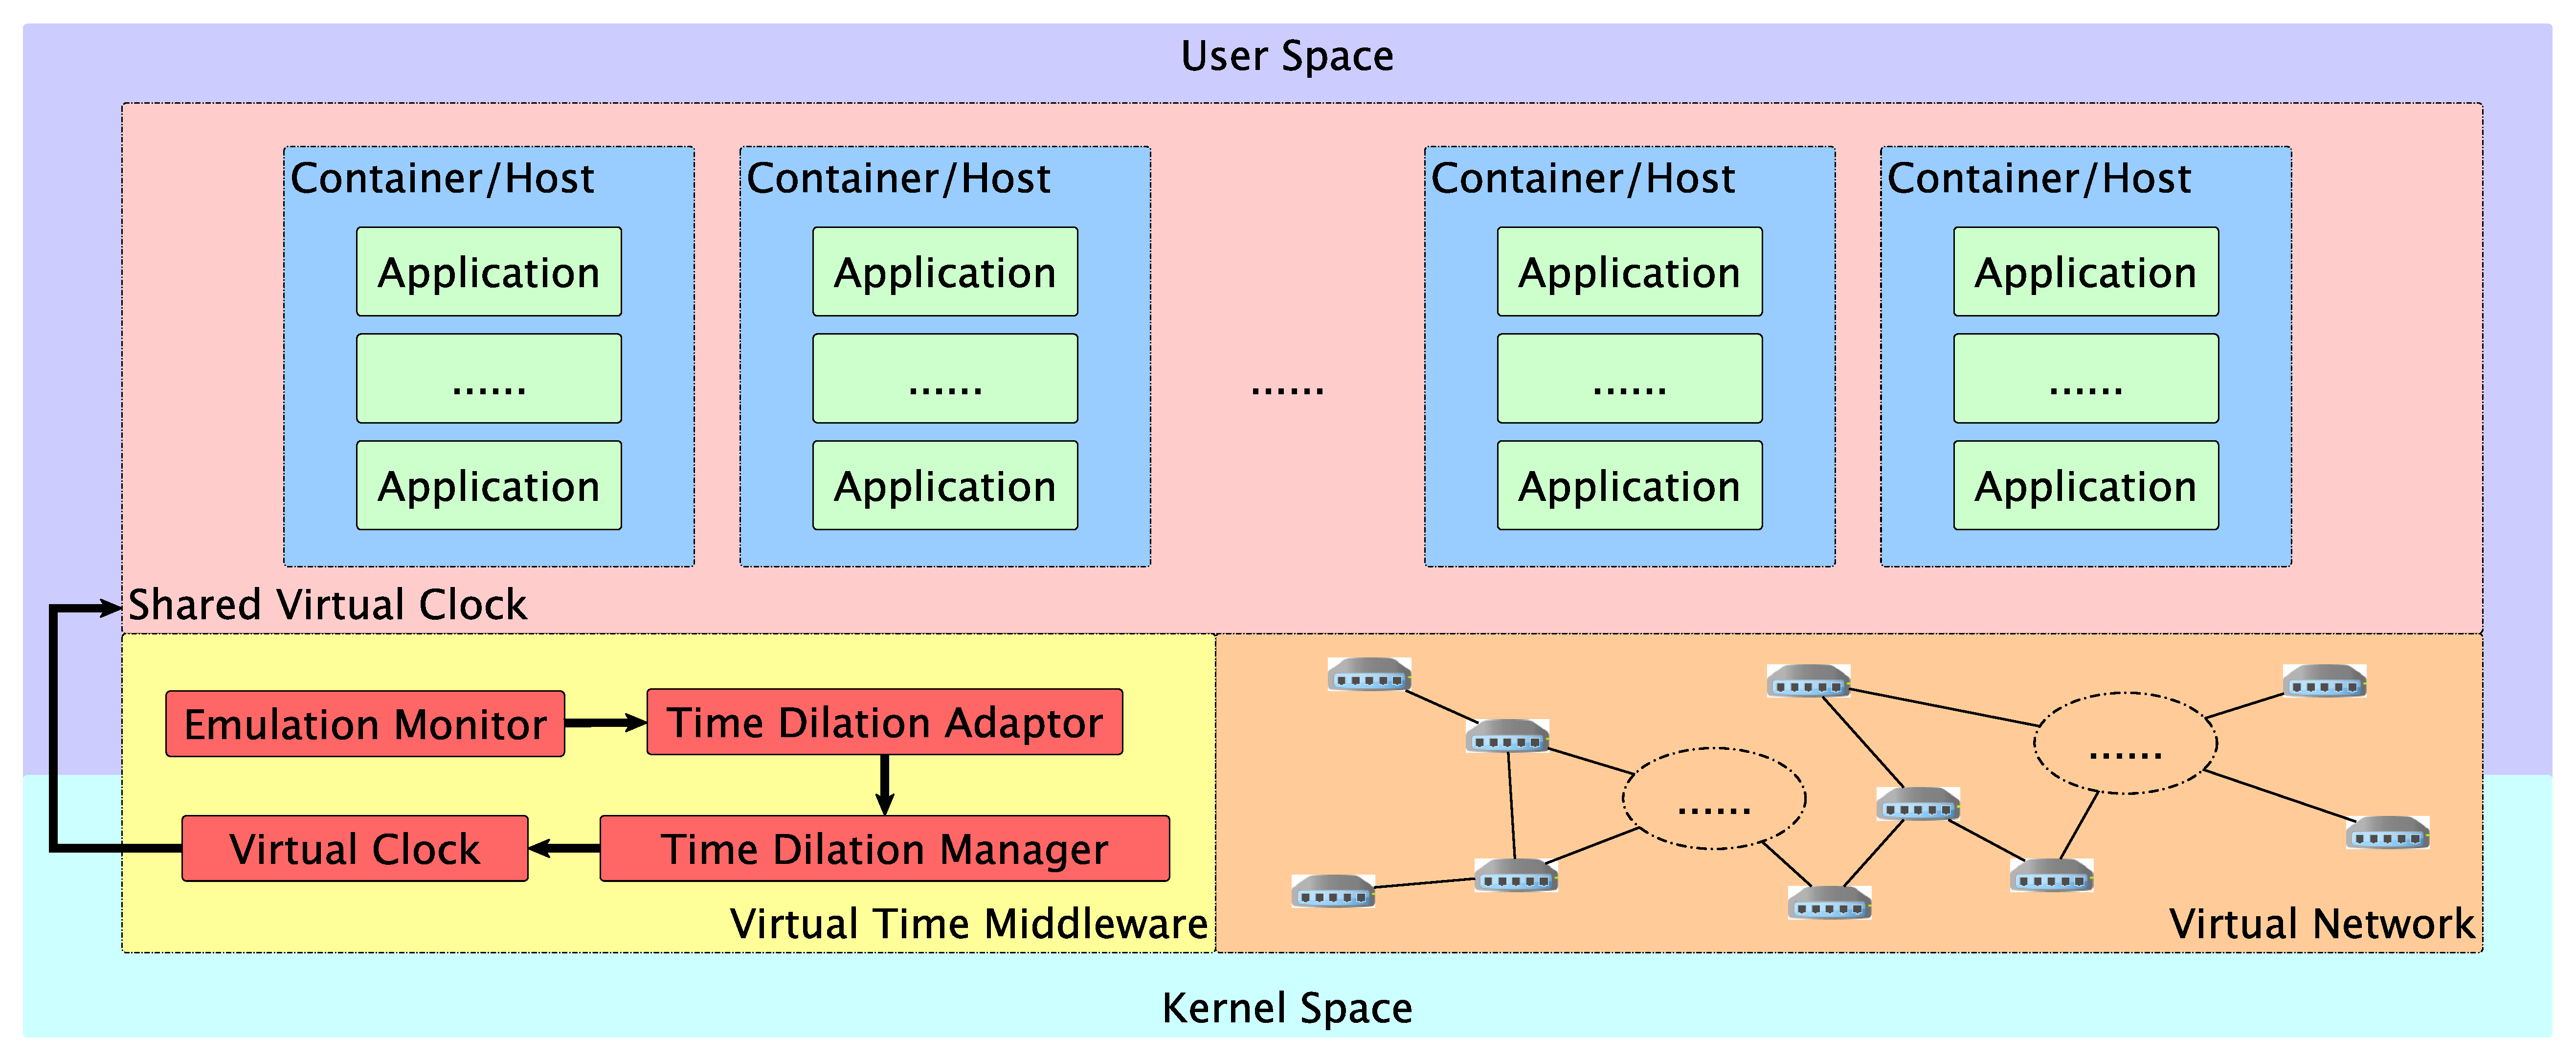
\epsfig{file=VirtualTime/figures/ContainerVirtualTime.eps, height=2in, width=5in}
\caption[Virtual Time System Design]{Architecture of the Virtual Time System in a Container-based Network Emulator.
    Note that a typical container-based network emulator can be presented by this figure without the Virtual Time Middleware.}
\label{VT:Fig:ContainerVirtualTime}
\end{figure*}

\Subsection{Virtual Time Management}
Our virtual time system, as shown in Figure~\ref{VT:Fig:ContainerVirtualTime}, is designed to meet all the requirements. 
The time dilation manager is responsible for computing and maintaining the virtual time, according to a given TDF for all the containers. 
It can offer per-container virtual time or the global virtual time for the emulator.
The per-container virtual time is useful to support synchronized emulation (in virtual time) and facilitates the integration with network simulators. 
We have made a small set of changes in the kernel, in particular, a modified data structure to present virtual time,
and a new algorithm to convert the elapsed wall-clock time to the dilated virtual time, with no dependency on third-party libraries.

We attach each container an integer-valued TDF, which could also be shared among all containers. 
A TDF of $k$ slows down a container's time advancement rate by a factor of $k$, thus re-scales a container's notion of time with reference to a physical network. 
This way, Mininet can emulate a seemingly $k$ times faster network owing to the accelerated rate of interaction between the containers and the virtual network
%When TDF is greater than 1, it appears to the containers that available resources including link bandwidth and CPU computation capacity are increased by a factor of TDF. 
Note that our design cannot scale the capacity of hardware components such as main memory, processor caches, and disk, firmware on network interfaces. 

The integration with Mininet, and potentially other container-based software is straightforward. 
We provide a set of simple APIs to (1) initialize containers with virtual time, and (2) inquire virtual time at run time. 
The system returns precise virtual time to container processes and transparently to all their child processes while returning the ordinary system time to other processes. 
We have integrated the system with Mininet. The implementation details are discussed in Section~\ref{VT:Sec:Implementation}, and we have madee our code base available to public on GitHub\footnote{see \href{https://github.com/littlepretty/VirtualTimeForMininet}{VirtualTimeForMininet}}. 

\subsection{Adaptive Time Dilation}
The key insight of virtual time is to trade time with available system resources.
The execution time can be unnecessarily long with an overestimated TDF. 
It is difficult to avoid that with a fixed TDF when the resource demands vary substantially during the emulation. 
Therefore, we investigate means to adaptively adjust TDF in run-time with the goal of well balancing the execution speed and accuracy. 
We take a similar epoch-based approach described in~\cite{NtwkEmultAdaptVirtTime}, and develop two modules,
Emulation Monitor and Time Dilation Adaptor (see Figure~\ref{VT:Fig:ContainerVirtualTime}), to achieve the dynamic TDF adjustment. 

Emulation Monitor periodically collects the process-related information (not necessarily coincides with the epoch duration)
and computes the run-time emulation load statistics, such as CPU utilization, number of waiting processes, or average process waiting time. 
Time Dilation Adaptor takes the inputs from Emulation Monitor, and adaptively computes the TDF for the next epoch based on a heuristic algorithm,
whose details are presented in Section~\ref{VT:Sec:Implementation}. 
Currently we only use the CPU utilization as the feedback control indicator, and will leave the exploration of other control algorithms as future works. 


\Section{Implementation}
\label{VT:Sec:Implementation}

The implementation of the virtual time system and its integration with Mininet-Hifi (the latest version of Mininet) is composed of three parts,
as shown in Figure~\ref{VT:Fig:VTMininetHifi}.
First, we built a lightweight and independent middleware in the Linux kernel to provide virtual time support to user-space software.
Second, we slightly modified the initialization procedure of Mininet with two additional python modules to realize (adaptive) virtual time in Mininet.
Third, we discuss our design to enable transparent support of virtual time for applications running in the containers.

\begin{figure}
    \centering
    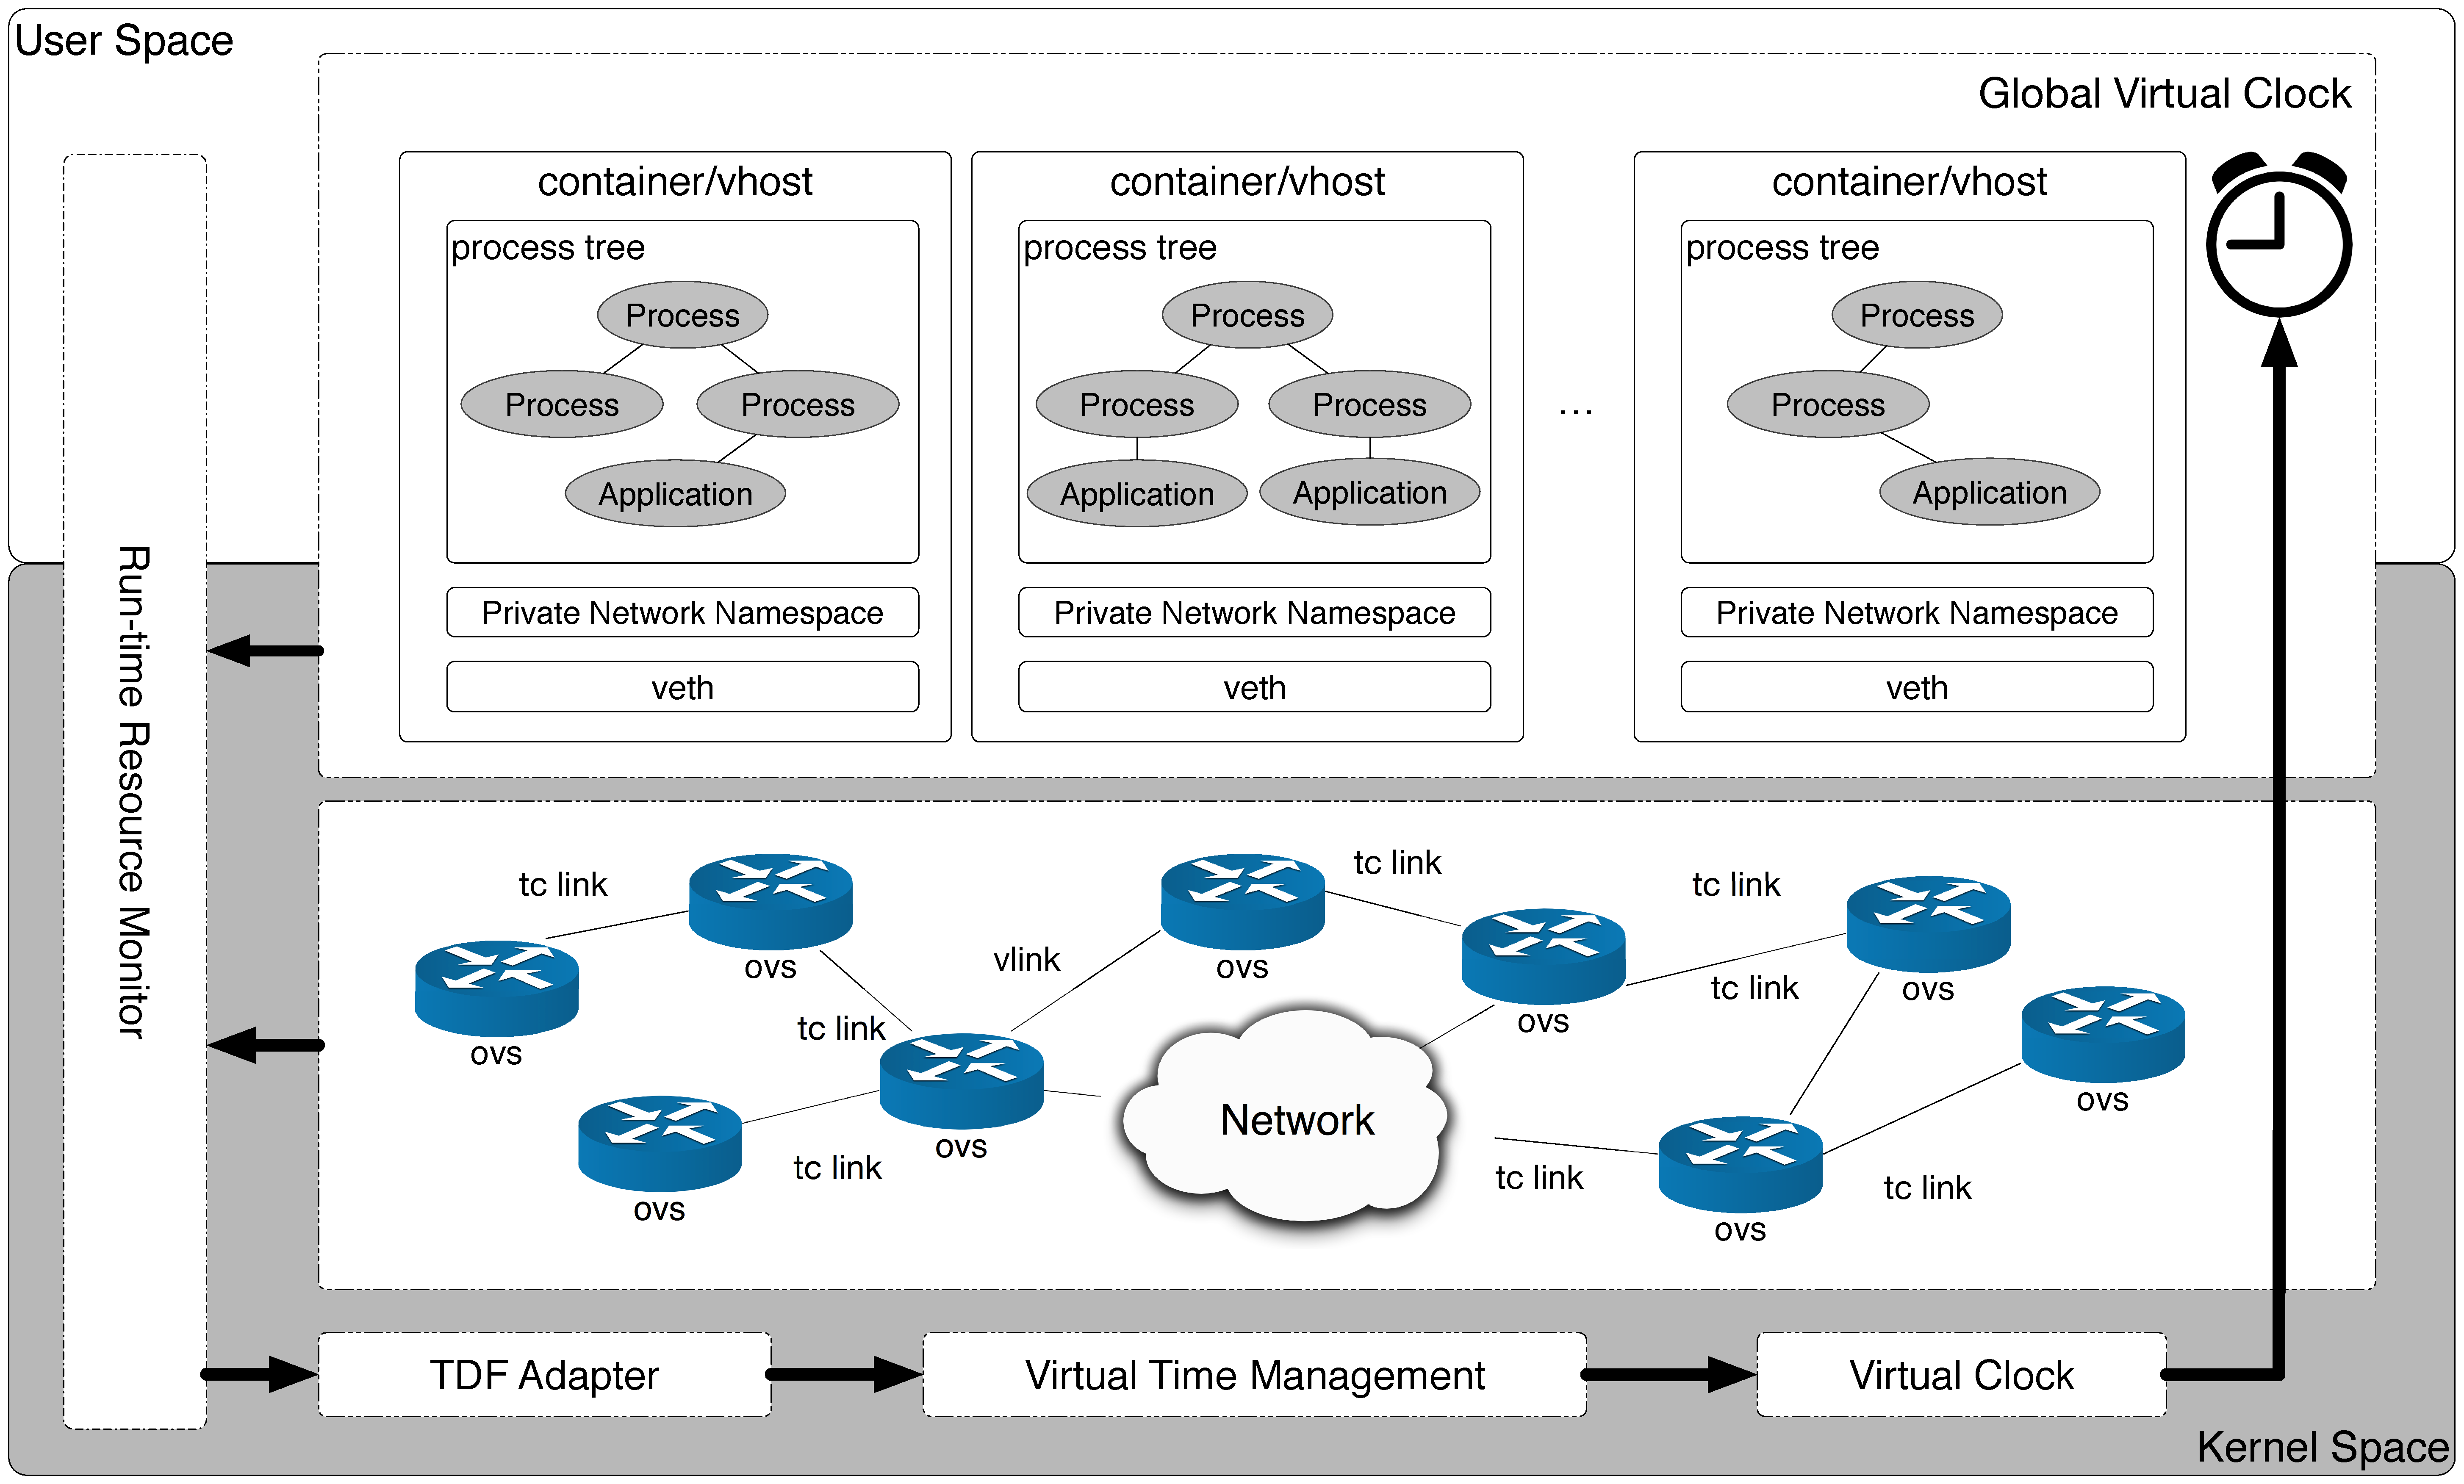
\epsfig{file=VirtualTime/figures/VT-Mininet-Hifi.eps, width=0.9\textwidth}
    \caption{Integration of Mininet-Hifi and Virtual Time}
    \label{VT:Fig:VTMininetHifi}
\end{figure}

\Subsection{Modification in Linux Kernel}
\paragraphbe{Timing-related Kernel Modifications.}
\label{VT:SubSec:ExtendLinuxKernel}
Our implementation is based on a recent Linux kernel 3.16.3 with no third-part library dependency.
To make a process have its own perception of time, we added the following four new fields in the \texttt{task\_struct} struct type.
\begin{itemize}
    \item \texttt{physical\_start\_ns} represents the starting time that a process detaches from the system clock and begins to use the virtual time, in nanoseconds.
    \item \texttt{physical\_past\_nsec} represents how much physical time has elapsed since the last time the process requested the current time, in nanoseconds
    \item \texttt{virtual\_start\_nsec} represents the starting time that a process detaches from the system clock and uses the virtual time, in nanoseconds 
    \item \texttt{virtual\_past\_nsec} represents how much virtual time has elapsed since the last time the process requested the current time, in nanoseconds
    \item \texttt{freeze\_start\_ns} represents the starting time that a process or a process group is frozen. It is always zero for a non-frozen process.
    \item \texttt{freeze\_past\_ns} represents the cumulative time, in nanoseconds, that a running process or a process group remains in the frozen state.
    \item \texttt{dilation} represents the TDF of a time-dilated process
\end{itemize}

\begin{algorithm}[ht]
    \DontPrintSemicolon
    \KwIn{$tk = $ C struct \texttt{task\_struct} representing a process in Linux kernel \newline
    $dilation = $ value of time dilation factor}
    \SetKwProg{Fn}{Function}{}{\KwRet}
    \SetKwFunction{InitVT}{init\_virtual\_time}
    \SetKwFunction{GetNS}{getnstimeofday}
    \SetKwFunction{TSNS}{timespec\_to\_ns}
    \Fn{\InitVT{$tk$, $dilation$}} {
        \If {$dilation > 0$} {
            $tk.virtual\_start\_nsec \gets 0$ \;
            $ts \gets$ \GetNS{} \;
            $tk.virtual\_start\_nsec \gets$ \TSNS{$ts$} \;
            $tk.virtual\_past\_nsec \gets 0$ \;
            $tk.physical\_past\_nsec \gets 0$ \;
            $tk.dilation \gets dilation$
        }
    }
    \caption{Initialize Virtual Time}
    \label{VT:Alg:InitVirtualTime}
\end{algorithm}

\begin{algorithm}[ht]
    \DontPrintSemicolon
    \KwIn {$p = $ the current running process in Linux kernel \newline
    $ts = $ current wall clock time \newline
    $tdf = p.dilation$}
    \SetKwProg{Fn}{Function}{}{\KwRet}
    \SetKwFunction{UpdatePPN}{update\_physical\_past\_nsec}
    \SetKwFunction{UpdateVPN}{update\_virtual\_past\_nsec}
    \SetKwFunction{DoDilate}{do\_virtual\_timekeeping}
    \SetKwFunction{TSNS}{timespec\_to\_ns}
    \SetKwFunction{NSTS}{ns\_to\_timespec}
    \Fn{\UpdatePPN{$ts$}} {
        $now \gets \TSNS{$ts$}$ \;
        $delta\_ppn \gets now - p.physical\_past\_nsec - p.physical\_start\_nsec - p.freeze\_past\_nsec$ \;
        $p.physical\_past\_nsec += delta\_ppn$ \;
        \KwRet{$delta\_ppn$} \;
    }
    \Fn{\UpdateVPN{$delta\_ppn$}} {
        $delta\_vpn \gets 0$ \;
        \If {$tdf > 0$} {
            $delta\_vpn \gets delta\_ppn / tdf$ \;
            $p.virtual\_past\_nsec += delta\_vpn$ \;
        }
        \KwRet{$delta\_vpn$}
    }
    \Fn{\DoDilate{$ts$}} {
        \If {$p.virtual\_start\_ns > 0$} {
            $delta\_ppn \gets \UpdatePPN{ts}$ \;
            $delta\_vpn \gets \UpdateVPN{delta\_ppn, tdf}$ \;
            $virtual\_now = p.virtual\_start\_nsec + p.virtual\_past\_nsec$ \;
            $virtual\_ts = \NSTS{virtual\_now}$ \; 
            $ts.tv\_sec = virtual\_ts.tv\_sec$ \;
            $ts.tv\_nsec = virtual\_ts.tv\_nsec$ \;
        }
    }
    \caption{Virtual Timekeeping Algorithm}
    \label{VT:Alg:VirtualTimeKeeping}
\end{algorithm}

\begin{algorithm}
    \DontPrintSemicolon
    \KwIn {$tsk = $ the process/container in Linux kernel to be frozen or unfrozen}
    \SetKwProg{Fn}{Function}{}{\KwRet}
    \SetKwFunction{Freeze}{freeze}
    \SetKwFunction{Unfreeze}{unfreeze}
    \SetKwFunction{PopulateFreeze}{populate\_frozen\_time}
    \SetKwFunction{KillGroup}{kill\_pgrp}
    \SetKwFunction{TaskGroup}{task\_pgrp}
    \SetKwFunction{GetNS}{getnstimeofday}
    \SetKwFunction{TSNS}{timespec\_to\_ns}
    \Fn{\Freeze{tsk}} {
        \KillGroup{\TaskGroup{tsk}, \texttt{SIGSTOP}, 1} \;
        $ts = $\GetNS{} \;
        $tsk.freeze\_start\_nsec \gets$ \TSNS{ts} \;
    }
    \Fn{\PopulateFreeze{tsk}} {
        \ForEach {child $\in$ tsk.children} {
            $child.freeze\_past\_nsec \gets tsk.freeze\_past\_nsec$ \;
            \PopulateFreeze{child} \;
        }
    }
    \Fn{\Unfreeze{$tsk$}} {
        $ts = $\GetNS{} \;        
        $now \gets$ \TSNS{ts} \;
        $tsk.freeze\_past\_nsec += now - tsk.freeze\_start\_nsec$ \;
        $tsk.freeze\_start\_nsec \gets 0$ \;
        \PopulateFreeze{tsk} \;
        \KillGroup{\TaskGroup{$tsk$}, \texttt{SIGCONT}, 1} \;
    }
    \caption{Freeze and Unfreeze Linux Container}
    \label{VT:Alg:Freeze}
\end{algorithm}


Algorithm~\ref{VT:Alg:InitVirtualTime} and~\ref{VT:Alg:VirtualTimeKeeping} give the details about how we implement the time dilation. 
To preserve an accurate virtual clock in the kernel, we added a private function \texttt{do\_virtual\_timekeeping}
in the Linux's timekeeping subsystem to keep tracking the dilated virtual time based on the physical time passed and TDF. 
Based on process's \texttt{virtual\_start\_nsec}, the system determines the type of time to return, i.e., the physical system clock time or the virtual time.

\texttt{virtual\_start\_nsec} in \texttt{init\_virtual\_time} should first be initialized to zero so that the next \texttt{gettimeofday}
always returns the undilated time to compute and record the exact physical time that a process starts to use virtual time.
To return the accurate virtual time upon requests, the duration since the last call to \texttt{do\_virtual\_timekeeping} is calculated and precisely scaled with TDF. 
To enable virtual time support for a wide range of timing-related system calls,
we extensively traced the routines in Linux's subsystems that request timing information (such as \texttt{getnstimeofday},
\texttt{ktime\_get}, \texttt{ktime\_get\_ts}, etc.), and modified them to properly invoke \texttt{do\_virtual\_timekeeping}.

The algorithm to freeze/unfreeze processes is shown in Algorithm~\ref{VT:Alg:Freeze},
and is implemented in the Linux kernel.
After stopping a group of processes, we record the  current time for calculating the process frozen duration once we unfreeze the process.
Note that sending \texttt{SIGCONT} to all processes is behind the time keeping function.
The reason is that if we resume the process group first, an unfrozen process may be scheduled to run,
and possibly query time before we complete populating the \texttt{freeze\_past\_ns} within the entire container.
We also develop a user space utility program \texttt{freeze\_all\_proc}.
This program can freeze and unfreeze multiple hosts in parallel.
In particular, it spawns one \texttt{pthread} for every network host to write its freeze entry in the Proc system.
Since the network emulator always pauses or resumes all hosts, this optimization significantly reduces the running overhead in large-scale network settings.

The virtual file system provides an interface between the kernel and the user space.
Since virtual time is a per-process property, it is more efficient to create a \texttt{/proc}
file entry for the associated processes rather than adding system calls.
The virtual time interface consists of two extra file entries under \texttt{/proc/\$pid}.
\begin{itemize}
    \item \texttt{/proc/\$pid/dilation} A process \texttt{\$pid} can enable and disable virtual time, as well as change a new time dilation factor (TDF).
        To support fractional dilation values, a TDF of $x$ is stored in this entry as $1000x$,  since floating point numbers are rarely supported in the Linux kernel.
    \item \texttt{/proc/\$pid/freeze} We can freeze and unfreeze a process \texttt{\$pid} according to the written boolean value.
        A value 1 freezes the entire process group and a value 0 resumes all the processes in this group.
\end{itemize}

We make a distinction between regular processes and virtual-time enabled processes. In other words, the \texttt{/proc/\$pid/freeze} entry is only valid only if \texttt{/proc/\$pid/dilation}  already has a non-zero value. The emulator can enable a container with virtual time by writing 1000 to the \texttt{dilation} proc file entry. This will turn on the freeze/unfreeze capability without unnecessarily modifying the clock speed. In this work, we use a process calling system call \texttt{unshare()} with flag \texttt{CLONE\_NEWTIME} to enable virtual time.
This design is motivated and tailored to be compatible with Mininet's programming interface.
\paragraphbe{Process-related Kernel Modifications.}
To enable the virtual time perception to processes running in a network emulator, we added the following new system calls.
\begin{itemize}
    \item \texttt{virtualtimeunshare} is essentially the \texttt{unshare} system call with time dilation inputs.
        It is used by container-based emulators, such as Mininet, to create emulated nodes.
        \texttt{virtualtimeunshare} creates a new process with a TDF in a different \texttt{namespace} of its parent process according to \texttt{flags}.
    \item \texttt{settimedilaitonfactor} offers an interface to change the TDF of a process.
        Note that a command executed in an emulated host is equivalent to forking a shell command executed by \texttt{bash}. 
        Therefore, adjusting a process' TDF requires the change of the calling process' parent (e.g., host's \texttt{bash}),
        which occasionally would lead to tracing back to the root of the process tree, especially in the case of dynamic TDF adjustment. 
\end{itemize}

We also modified the \texttt{do\_fork} system call to initialize the virtual-time-related attributes of a process,
such as using the variable \texttt{stack\_size} to pass the TDF value. 
Another option is to set TDF to a default value in \texttt{virtualtimeunshare} and
then relies on explicitly invoking \texttt{settimedilationfactor} to set desired TDF;
this method prevents modifying the interface of creating \texttt{namespace} in traditional Linux. 
Functions in \texttt{timekeeping.c} were modified to invoke \texttt{do\_dilatetimeofday}
in order to return the virtual time to system calls like \texttt{gettimeofday} and other kernel routines that request timing information.


\paragraphbe{Networking-related Kernel Modifications.}
In this work, we focus on capturing all the related system calls and kernel routings to support virtual time in Linux container with the application of Mininet. 
One particular case related to Mininet is the usage of \texttt{tc}, a network quality-of-service control module in Linux~\cite{TrafficControl}. 
For instance, we can use \texttt{tc} to rate-limit a link to 100 Mbps using Hierarchic Token Bucket (HTB) \texttt{qdisc} in Mininet. If the TDF is set to 8, the link bandwidth would be approximately 800 Mbps from the emulated hosts' viewpoints as we observed from the time-dilated \texttt{iperf3} application.

As a network module in Linux, \texttt{tc} does not reference Linux kernel's time as the way user application does. 
Therefore, \texttt{tc} is transparent to our virtual time system. One way to solve this problem is to modify the network scheduling code in kernel to provide \texttt{tc} with a dilated traffic rate. 
In the earlier example with TDF set to 8, the experiment will run 8 times slower than the real time, and we can configure \texttt{tc}'s rate limit as $rate/TDF=12.5$ Mbps to emulate a 100 Mbps link. 
Note that we only tailored HTB in \texttt{tc}, which is the default \texttt{qdisc} used by Mininet. 
We will generalize the mechanism to other \texttt{qdiscs} including HFSC (Hierarchical Fair Service Curve) and TBF (Token Bucket Filter) in the future.

\Subsection{Modification in Network Emulator}
\paragraphbe{Virtual-Time-Enabled Mininet.}
\label{VT:SubSec:ImplementMininet}
%Mininet uses Linux's container \cite{LXC} to enable scalable network emulation. 
Containers allow groups of process running on the same kernel to have independent views of system resources, such as process IDs, file systems and network interfaces. 
We add the virtual time property to a container's \texttt{namespace}~\cite{LinuxNamespace} so that every container can have its own virtual clock. 
We design our system in the way that minimal modifications of Mininet are needed for integration, so that the virtual time system can be easily extended to other Linux-container-based applications. 

We modified the initialization procedure of Mininet, in particular, the \texttt{mnexec} program in Mininet, to process two additional parameters. 
When we create \texttt{Node}s in Mininet (hosts, switches, and controllers are all inherited from \texttt{Node}), users can feed in a TDF argument with \texttt{virtualtimeunshare} (as a replacement of \texttt{unshare}) with \texttt{-n} option. 
This way, a system-wide TDF can be conveniently set for all the emulated hosts. We also provide the ability to dynamically adjust the TDF for every emulated host during runtime. 
To do that, we added a new option \texttt{-t} in \texttt{mnexec} to invoke the aforementioned system call \texttt{settimedilaitonfactor} to do the actual TDF adjustment. 
The two modifications enable the integration of virtual time in Mininet, and also serve as the basis of the adaptive TDF management.

\paragraphbe{Adaptive TDF Scheduling.}
To optimize the performance of the virtual-time-enabled Mininet, we developed an adaptive TDF scheduler
through two python modules \texttt{MininetMonitor} and \texttt{DilationAdaptor}
(refer to Emulation Monitor and Time Dilation Adaptor in Figure~\ref{VT:Fig:ContainerVirtualTime})
to accelerate the experiment speed while preserving high fidelity.

\texttt{MininetMonitor} is responsible to monitor the CPU usage of the entire emulation system,
consisting of a group of processes including the Mininet emulator, the Open vSwitch module, and emulated nodes (e.g., SDN controllers, hosts and switches). 
Also, applications are dynamically created, executed and destroyed within containers, in the form of child processes of their parent containers. 
\texttt{MininetMonitor} utilizes the \texttt{ps} command to collect the group's aggregate CPU percentage
and periodically computes and passes the average CPU load statistics to \texttt{DilationAdaptor}. 
The core of \texttt{DilationAdaptor} is an adaptive algorithm to calculate an appropriate \textit{TDF}.
%Only after receiving a new \textit{TDF} can Mininet pause the experiment and update its global time dilation factor. Otherwise it enters the next Epoch directly. 
Global \textit{TDF} updating was achieved by invoking the \texttt{mnexec\ -t\ tdf} program for every running host. 


% Algorithm \ref{Alg-AdaptiveTDF} illustrates our adaptive TDF scheduling, and we implemented it as a threshold-based \texttt{DilationAdaptor}. 
% %From the input fed by \texttt{MininetMonitor}, \texttt{DilationAdaptor} first define current load status. The key idea here is: if emulator is overloaded, we increase TDF with a large value; if it is underloaded, we may consider decrease TDF with a large value. 

% \algnewcommand\algorithmicswitch{\textbf{switch}}
% \algnewcommand\algorithmiccase{\textbf{case}}
% \algnewcommand\algorithmicassert{\texttt{assert}}
% \algnewcommand\Assert[1]{\State \algorithmicassert(#1)}%
% % New "environments"
% \algdef{SE}[SWITCH]{Switch}{EndSwitch}[1]{\algorithmicswitch\ #1\ \algorithmicdo}{\algorithmicend\ \algorithmicswitch}%
% \algdef{SE}[CASE]{Case}{EndCase}[1]{\algorithmiccase\ #1}{\algorithmicend\ \algorithmiccase}%
% \algtext*{EndSwitch}%
% \algtext*{EndCase}%

% \algrenewcommand{\algorithmiccomment}[1]{\hskip1em$/*$ #1 $*/$}
% \begin{algorithm}
% \caption{Adaptive Time Dilation Factor Scheduling}\label{Alg-AdaptiveTDF}
% \begin{algorithmic}[1]
% \State{Decide emulation $state$ through the resource indicator}\Comment{e.g., CPU utilization}
% \State{$MAX$ denotes the maximum allowed TDF value.}
% \State{$\Delta_{large}, \Delta_{small}$ denote the customizable large and small adjustment}
% \Switch{$state$}
% 	\Case{$OVERLOADED$}
% 		\State{$TDF_{new}=TDF_{prev}+\Delta_{large}$}
% 	\EndCase
% 	\Case{$WARNING$}
% 		\State{$TDF_{new}=TDF_{prev}+\Delta_{small}*2$}
% 	\EndCase
% 	\Case{$MODERATE$}
% 		\If{$TDF_{prev} == MAX$}
% 			\State{$TDF_{new}=TDF_{prev}-\Delta_{large}$}
% 		\ElsIf{$TDF_{prev} > \Delta_{small}$}
% 			\State{$TDF_{new}=TDF_{prev}-\Delta_{small}$}
% 		\Else
% 			\State{$TDF_{new}=TDF_{prev}$}%\Comment{Do not change TDF}
% 		\EndIf
% 	\EndCase
% 	\Case{$LIGHT$}
% 		\If{$TDF_{prev} > \Delta_{large}*2$}
% 			\State{$TDF_{new}=TDF_{prev}-\Delta_{large}$}
% 		\Else
% 			\State{$TDF_{new}=TDF_{prev}-\Delta_{small}*2$}
% 		\EndIf
% 	\EndCase
% \EndSwitch
% %\State{return $TDF_{new}$}
% \end{algorithmic}
% \end{algorithm}

Our adaptive virtual time scheduling design is similar to the one used in~\cite{NtwkEmultAdaptVirtTime} in spirit with two major differences. 
First, both techniques target on different platforms. 
Our technique is applied to Linux-container-based network emulation to support scalable SDN experiments,
and theirs uses virtual routing and executes OpenVZ instances inside Xen. 
Second, their solution needs be deployed on a cluster to emulate a medium-scale network, which results in much higher communication overhead in two types:
(1) every VM's monitor needs to report the CPU usage, and
(2) the adaptor needs to send new TDF to every VM. 
Therefore, the message transmission delay in LAN and the processing delay in protocol stacks contributes to the overall communication delay. 
In contrast, \texttt{MininetMonitor} runs as a lightweight background thread in Mininet,
and \texttt{DilationAdaptor} is simply a python object that Mininet has a reference to. 
The communication in our system is through synchronized queues and method invocations, which is much faster. 

\Subsection{Virtual Time Support for Network Applications}
\label{VT:SubSec:ModificationApplications}
Network applications running inside containers (e.g., \texttt{iperf3}~\cite{iperf3} or \texttt{ping}) should also use virtual time. 
We do not need to modify the application code because they are running as child processes of Mininet's hosts. 
A child process always copies its parent's \texttt{task\_struct} when it is forked including the same \texttt{dilation} and \texttt{virtual\_start\_nsec} values. 
Although \texttt{virtual\_start\_nsec} does not present the virtual starting time of the child process,
our algorithm is designed to work with relative values since it does necessary initial processes during \texttt{do\_fork}. 
When applications inquire about the system time,
the modified kernel knows that they are using virtual clock and return the virtual clock time instead of the system clock time.

One issue we notice is that the 64-bit Linux kernel running on Intel-based architectures provides the Virtual Dynamic Shared Object (vDSO)
and the \texttt{vsyscall} mechanism to reduce the overhead of context switches caused by the frequently invoked system calls,
for example, \texttt{gettimeofday} and \texttt{time}~\cite{VDSO}. 
Therefore, applications may bypass our virtual-time-based system calls unless we explicitly use the \texttt{syscall} function.
Our solution is to disable vDSO with respect to \texttt{\_\_vdso\_gettimeofday} in order to transparently offer virtual time to applications in the containers.


\Section{Evaluation}
\label{VT:Sec:Experiments}

In this section, we give experimental results to validate our implementation of the virtual time supported Mininet-Hifi network emulator.
Very straightforward but nontrivial network typologies are adopted to demonstrate
that the emulation system described in~\ref{VT:Sec:Implementation} can improve fidelity, scalability as well as efficiency. 

All the experiments are conducted on a Dell XPS 8700 Desktop with one Intel Core i7-4790 CPU,
12 GB RAM and one gigabit Ethernet interface. The machine runs a 64-bit Ubuntu 14.04.1 LTS with our customized 3.16.3 Linux kernel.
The benchmark scores of this machine's CPU and FPU are: 1.52 seconds for Blowfish, 1045.62 MiB/seconds for CryptoHash,
0.63 seconds for FFT and 2.56 seconds for Raytracing. Our virtual-time-enabled Mininet was built on the latest version of Mininet (2.1.0),
also named Mininet-Hifi, at the time of development.

\Subsection{Fidelity}
We first evaluate how our virtual time system improves Mininet's fidelity through a basic network scenario:
a single TCP flow transmission through a chain of switches in an emulated SDN network.
As shown in Figure~\ref{VT:Fig:ChainTopoExample}, the network topology consists of a client-server pair connected by a chain of Open vSwitch switches in Mininet.
We setup the default OpenFlow controller to function as a learning switch.
In this set of experiments, we connected two hosts through 40 switches in Mininet, and all the links are configured with 10 $\mu s$ delay.
We used \texttt{iperf3}~\cite{iperf3} to generate a TCP flow between the client and the server.
TDF was set to 1 (i.e., no virtual time) and 4 for comparison. We also setup a real testbed for ``ground truth" throughput data collection.
The testbed was composed of two machines connected by a 10 Gbps Ethernet link.
We varied the bandwidth link from 100 Mbps to 10 Gbps and measured the throughput using \texttt{iperf3}.
In the real testbed, we manually configured the link bandwidth and delay using \texttt{tc},
and the delay was set as the corresponding round trip times (RTTs) measured in the switch chain topology in Mininet,
so that the networking settings were tightly coupled for comparison.
Although we did not setup an exact network with SDN switches,
the stabilized TCP throughputs generated by the physical testbed should reflect what occurs in a real SDN network.
Each experiment was repeated 10 times and the results with bandwidth 4 Gbps, 8 Gbps and 10 Gbps were reported in Figure~\ref{VT:Fig:Perf40SwDiffBw}. 

We observe that when the bandwidth was no greater than 4 Gbps (we only displayed the 4 Gbps case in the figure),
Mininet was able to accurately emulate the TCP flow with and without virtual time,
as the average throughputs were very close to the ones collected from the physical testbed.
However, when we continued to increase the bandwidth, Mininet was not able to produce the desired throughputs, e.g.,
28\% (8 Gbps) and 39\% (10 Gbps) smaller than the physical testbed throughputs.
With virtual time (TDF = 4), Mininet was capable to accurately emulate the TCP flow even at high bandwidth,
and the results were nearly the same as the ones measured in the physical testbed. 

The root cause is that the machine running Mininet does not have sufficient resources to emulate networks with bandwidth greater than 4 Gbps,
which would lead to fidelity issues, e.g., low expected throughputs.
Note that we only emulated a single flow, and the results could be much worse and unpredictable in complicated multi-flow scenarios.
Results show that virtual time can significantly enhance the performance fidelity
by ``slowing down" the experiments so that the system has sufficient resources and time to correctly process the packets.
We further illustrate the effect by plotting the time series of throughput changes for the 10 Gbps cases in Figure~\ref{VT:Fig:Perf40Sw10GbLink}.
With virtual time, the throughputs measured in Mininet closely match the real testbed results;
without virtual time ($TDF = 1$), the ramp up speed was much slower, in particular,
22 seconds ($TDF = 1$) rather than 4 seconds ($TDF = 4$), and the throughput was incorrectly stabilized below 6.1 Gbps.

\Subsection{Scalability}
Virtual time also improves the scale of networks that one can emulate without losing fidelity.
In this set of experiments, we used the same switch chain topology in Figure~\ref{VT:Fig:ChainTopoExample},
and set the link bandwidth to 4 Gbps. We want to investigate, with virtual time,
how many switches Mininet is capable to emulate without losing fidelity, i.e., preserving nearly 4 Gbps throughput.
This time we increased the number of switches with the following values \texttt{\{20, 40, 60, 80, 100\}},
and TDF was selected to be 1 (no virtual time) and 4. We ran \texttt{iperf3} for 25 seconds between the client and the server.
Each experiment was repeated ten times, and the throughput measurement is reported in Figure~\ref{VT:Fig:ScaleDiffSw4GbLink}.

In the case of $TDF = 1$, the average throughput kept decreasing as the number of switches grew over 20.
The throughput decreased dramatically when the number of switches was greater than 60 (e.g., decreased by 41\% for 60 switches, 65\% for 80 switches, and 83\% for 100 switches).
The standard deviation, indicated the undesired high disturbance, also grew as number of switches increased.
When virtual time was applied with $TDF = 4$, the throughput was always around 3.8 Gbps with small standard derivations in all the experiments.
It is clear that virtual time helps to scale up the emulation.
In this case, Mininet can emulate 100 switches with 4 Gbps links and still generate the accurate throughputs,
rather than being saturated at 20 switches without virtual time. 

We also recorded the running time in Figure~\ref{VT:Fig:ScaleTime}.
Longer execution time is the tradeoff for the fidelity and scalability improvement.
When $TDF=4$, the execution time was about 4 times longer than the time required in the case of $TDF=1$ in all the experiments.
In fact, we have conducted extensive experiments with different TDF values on multiple network scenarios.
The general observation is that a larger TDF allows an emulator to conduct accurate experiments with larger scale on the same physical machine,
but typically requires longer execution time, approximately proportional to the TDF.
This leads to the question on how to balance the speed and fidelity,
and our approach is to explore the adaptive time dilation scheduling, whose evaluation is presented in the next section. 

\begin{figure}
    \centering
    \subfigure[Chain Network Topology]{{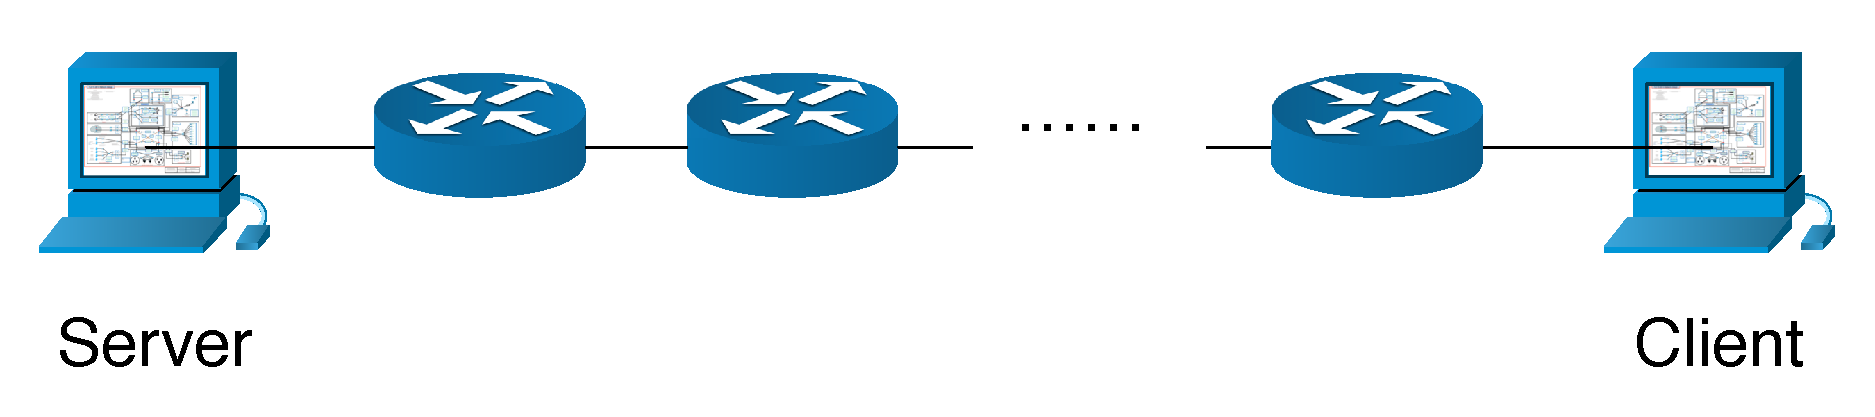
\epsfig{file=VirtualTime/figures/TopoChainExample.eps, width=0.45\textwidth}}
    \label{VT:Fig:ChainTopoExample}}
    \subfigure[Linear Network Topologies]{{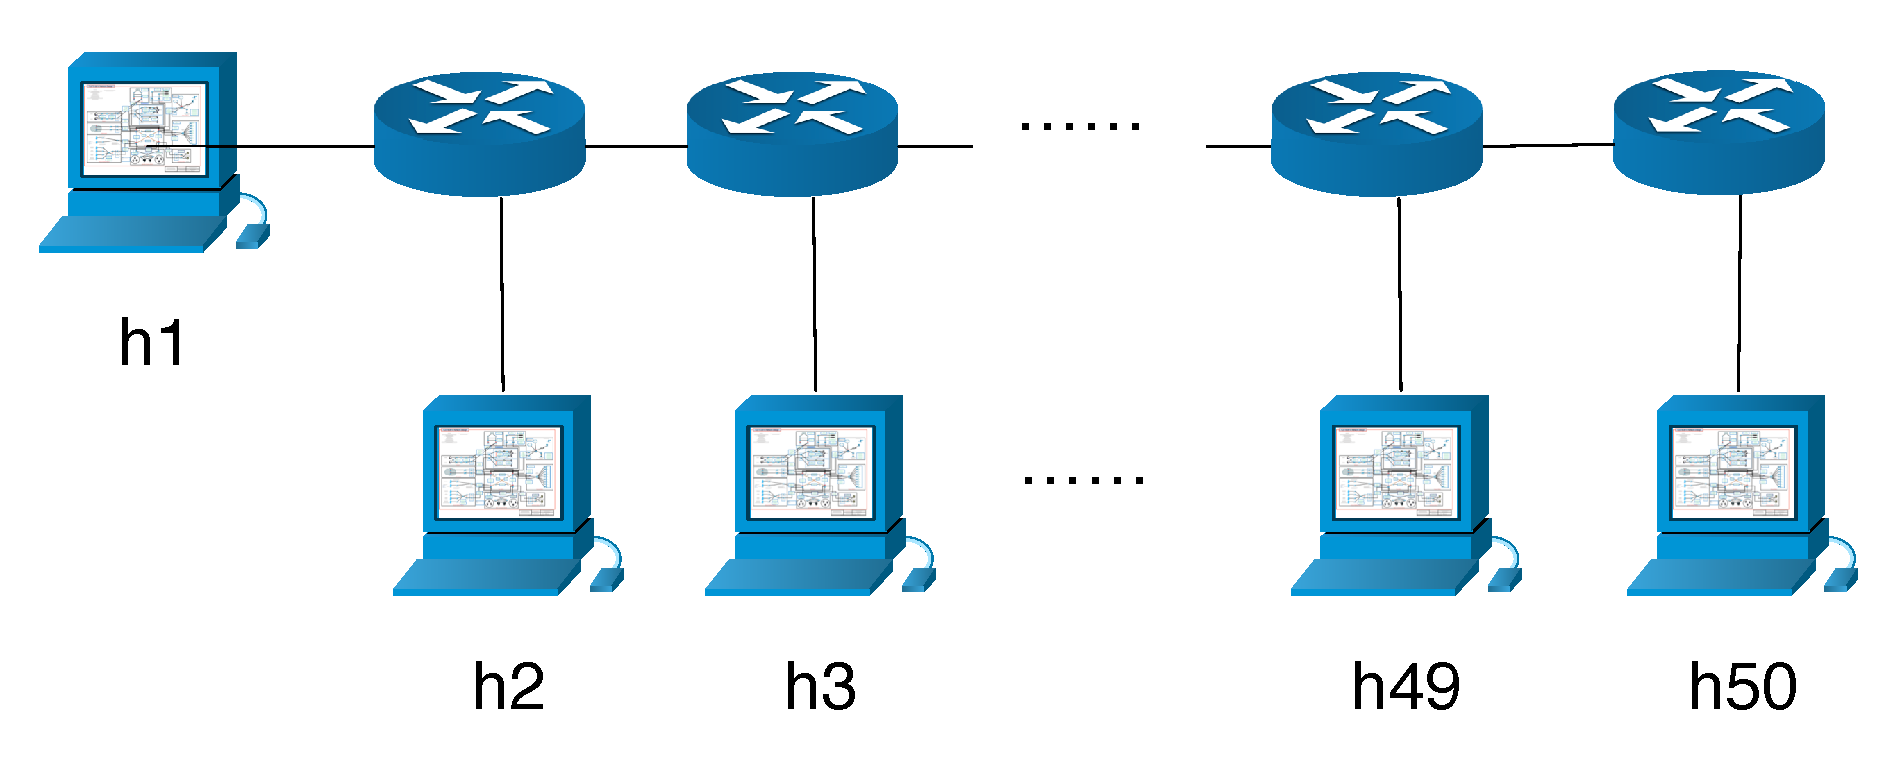
\epsfig{file=VirtualTime/figures/TopoLinearExample.eps, width=0.45\textwidth}}
    \label{VT:Fig:LinearTopoExample}}
    \caption{Network Topologies Used in Virtual Time Evaluation}
\end{figure}

\begin{figure}
    \centering
    \subfigure[TCP Throughput with Different Link Bandwidths]{{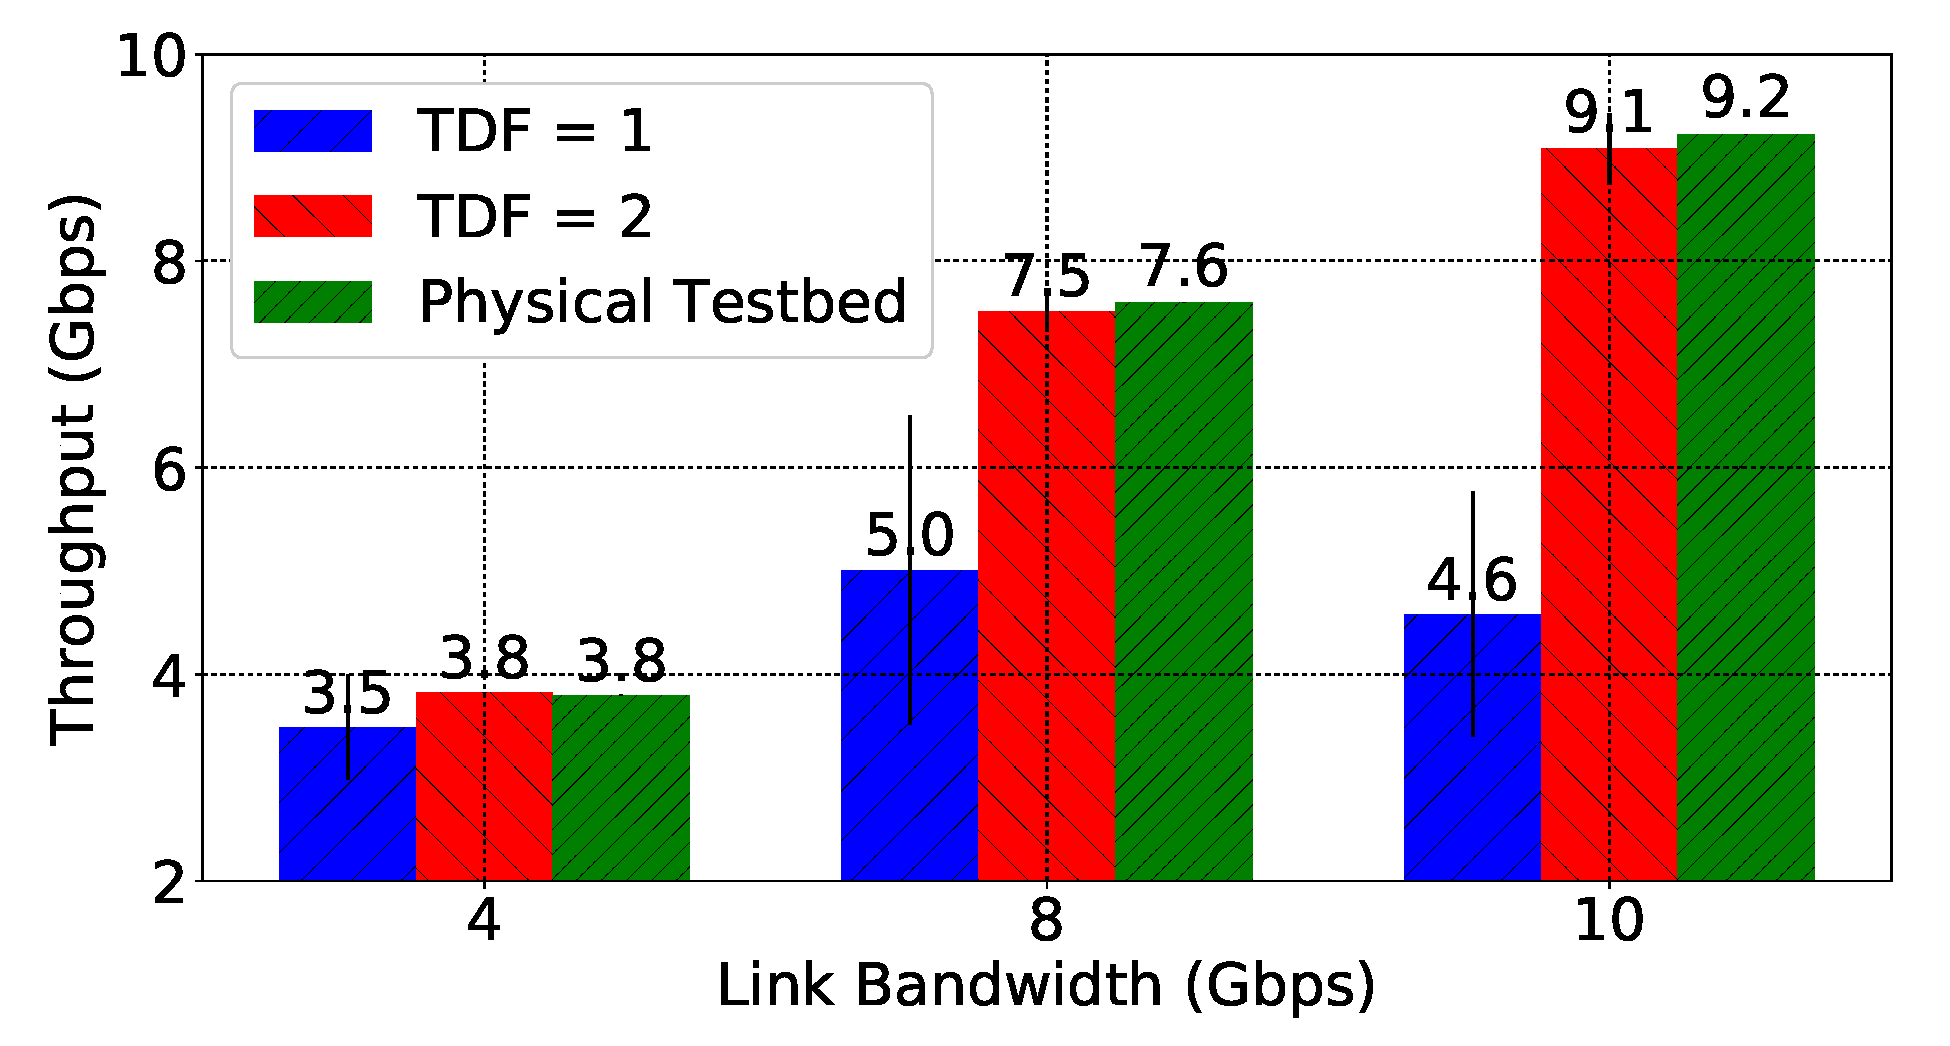
\epsfig{file=VirtualTime/figures/Perf40SwDiffBw.eps, width=0.45\textwidth}}
    \label{VT:Fig:Perf40SwDiffBw}}
    \subfigure[TCP Throughput with 10 Gbps Links]{{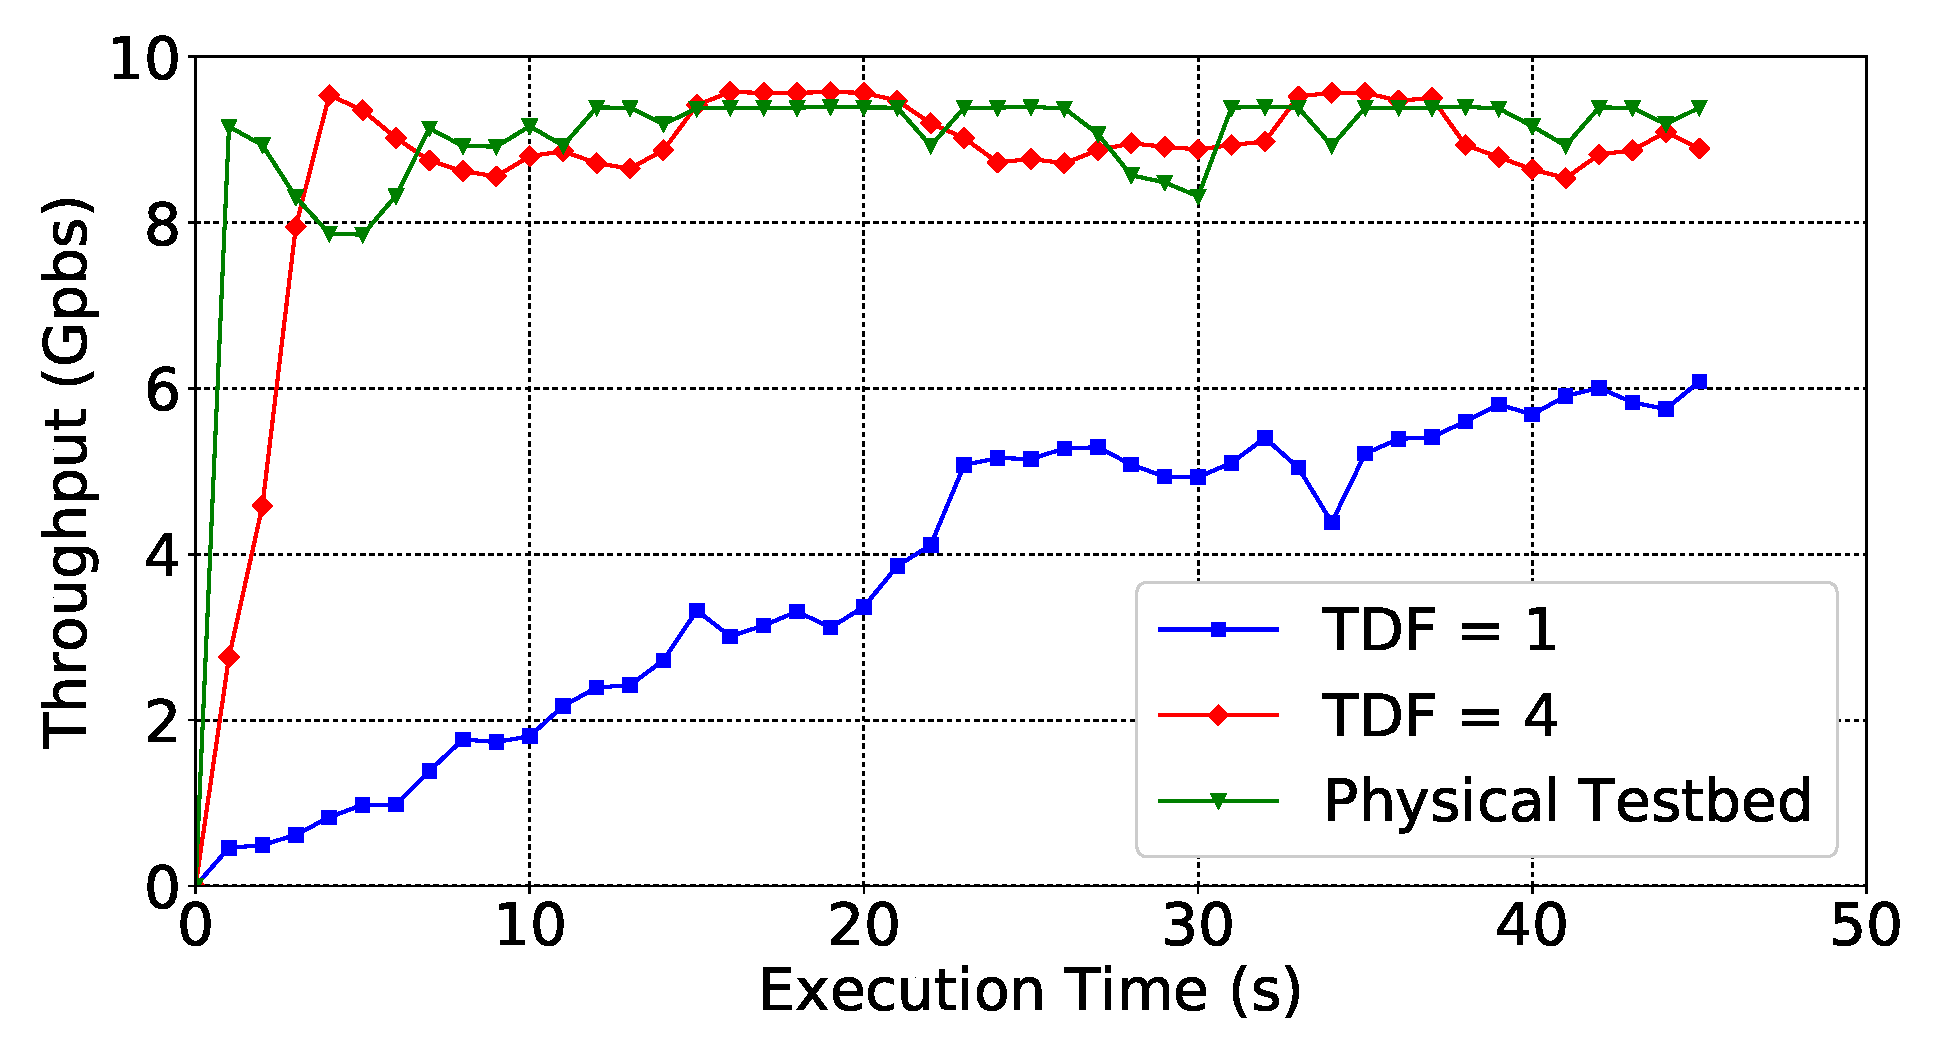
\epsfig{file=VirtualTime/figures/Perf40Sw10GbLink.eps, width=0.45\textwidth}}
    \label{VT:Fig:Perf40Sw10GbLink}}
    \caption{Fidelity Evaluation Experimental Results}
\end{figure}

\begin{figure}
    \centering
    \subfigure[TCP Throughput]{{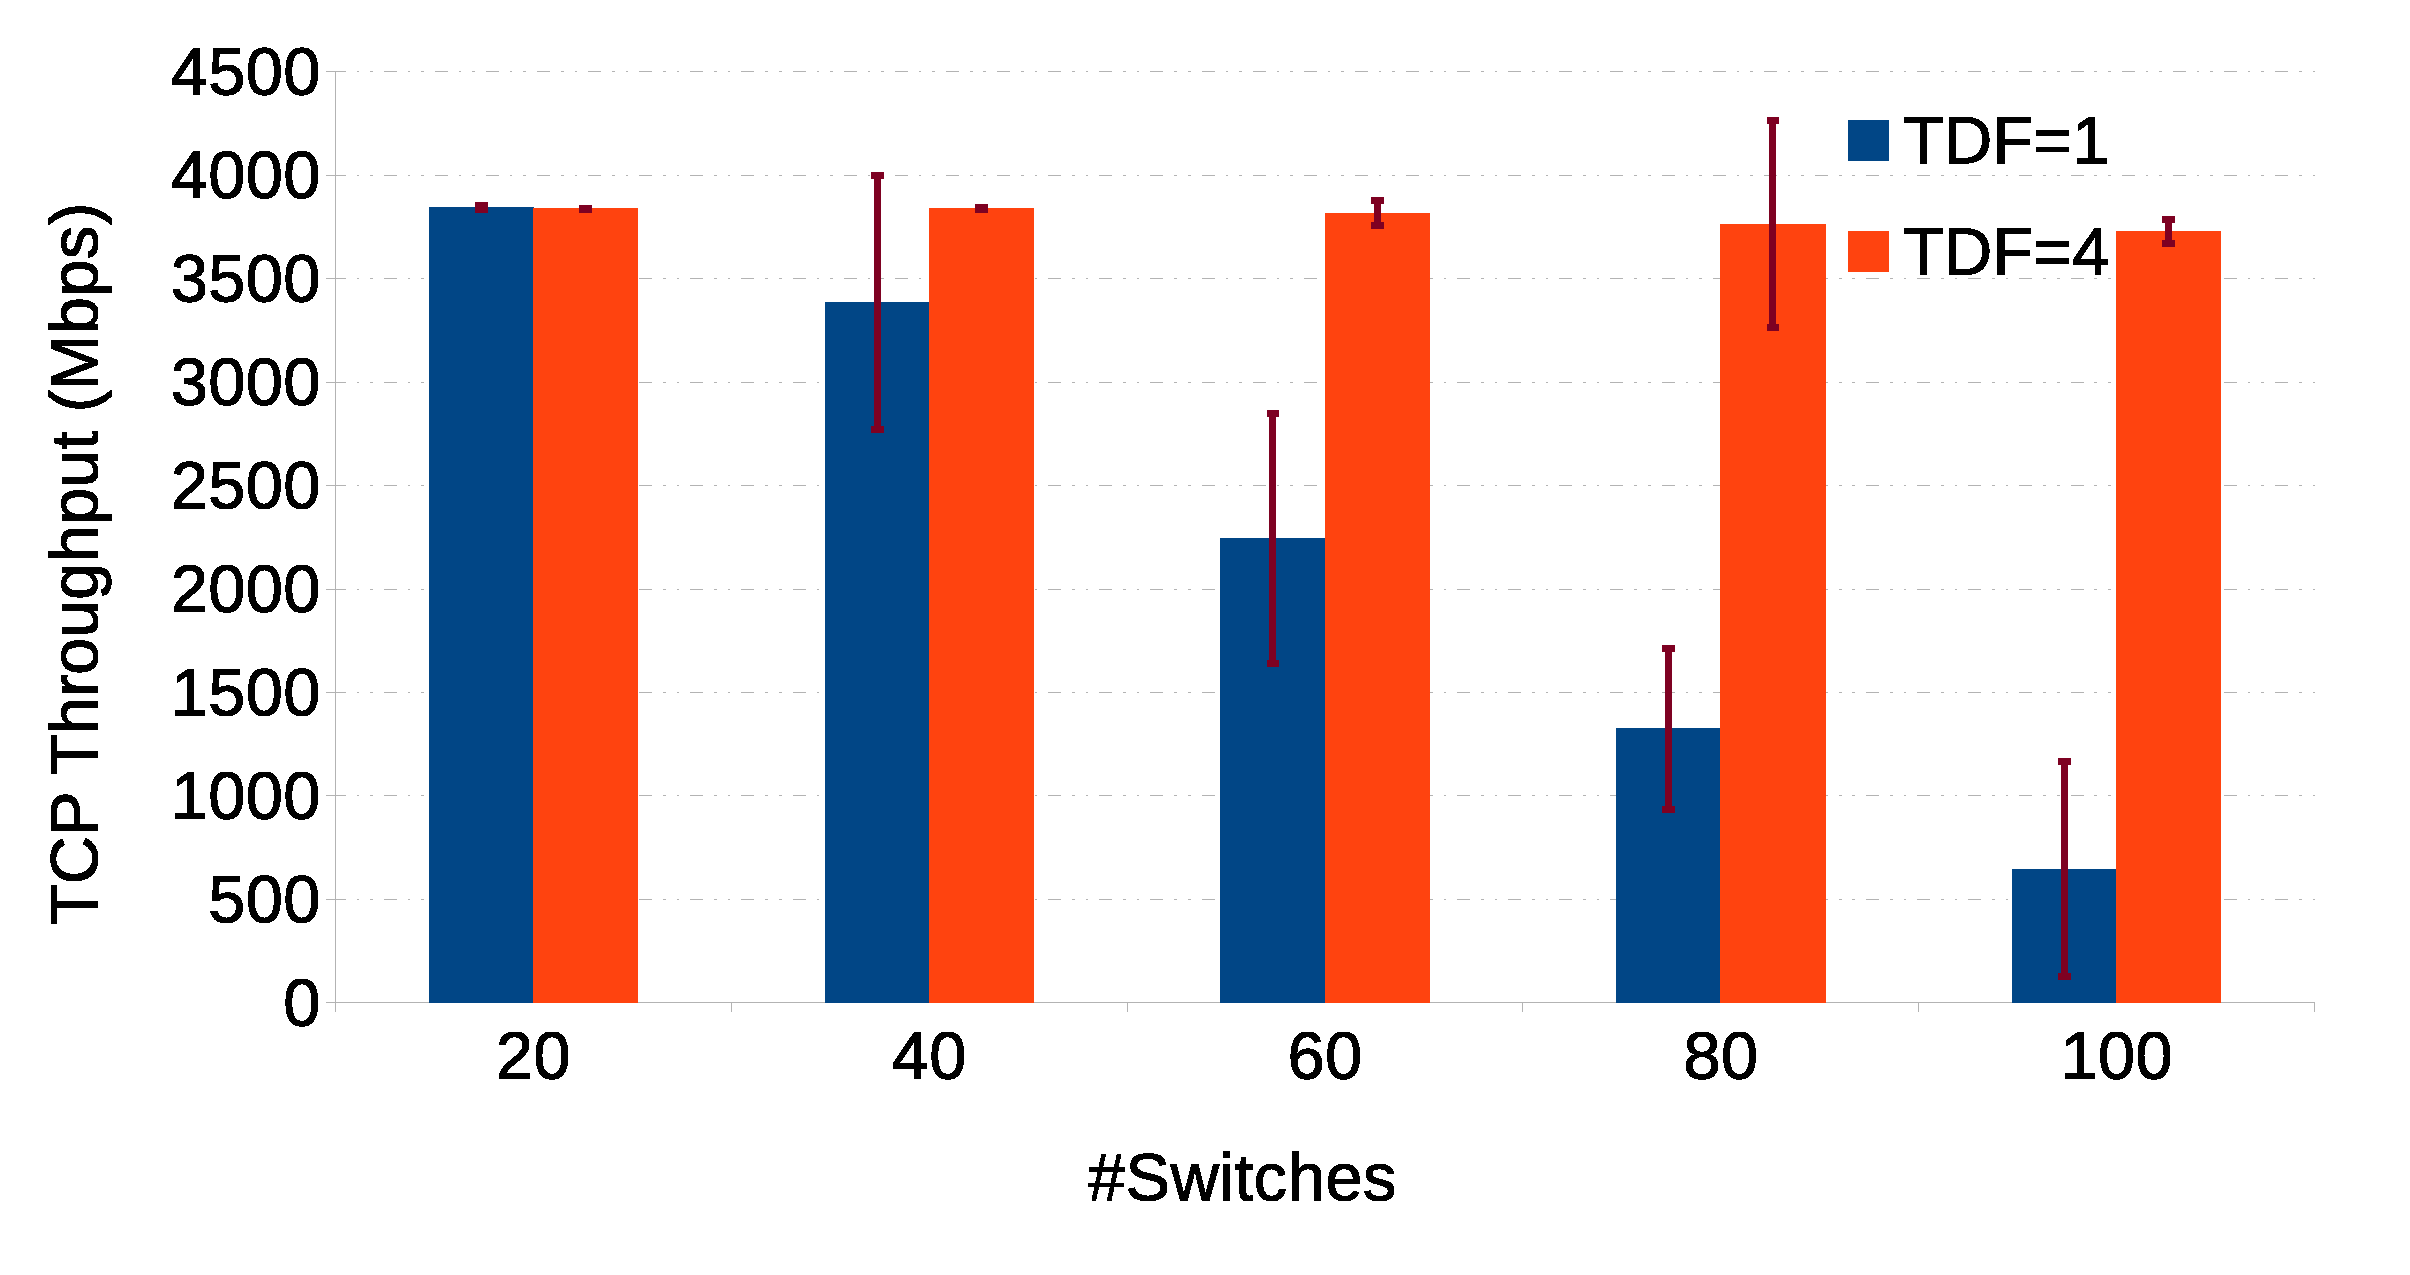
\epsfig{file=VirtualTime/figures/ScaleDiff100Sw4GbLink.eps, width=0.45\textwidth}}
    \label{VT:Fig:ScaleDiffSw4GbLink}}
    \subfigure[Evaluation Running Time]{{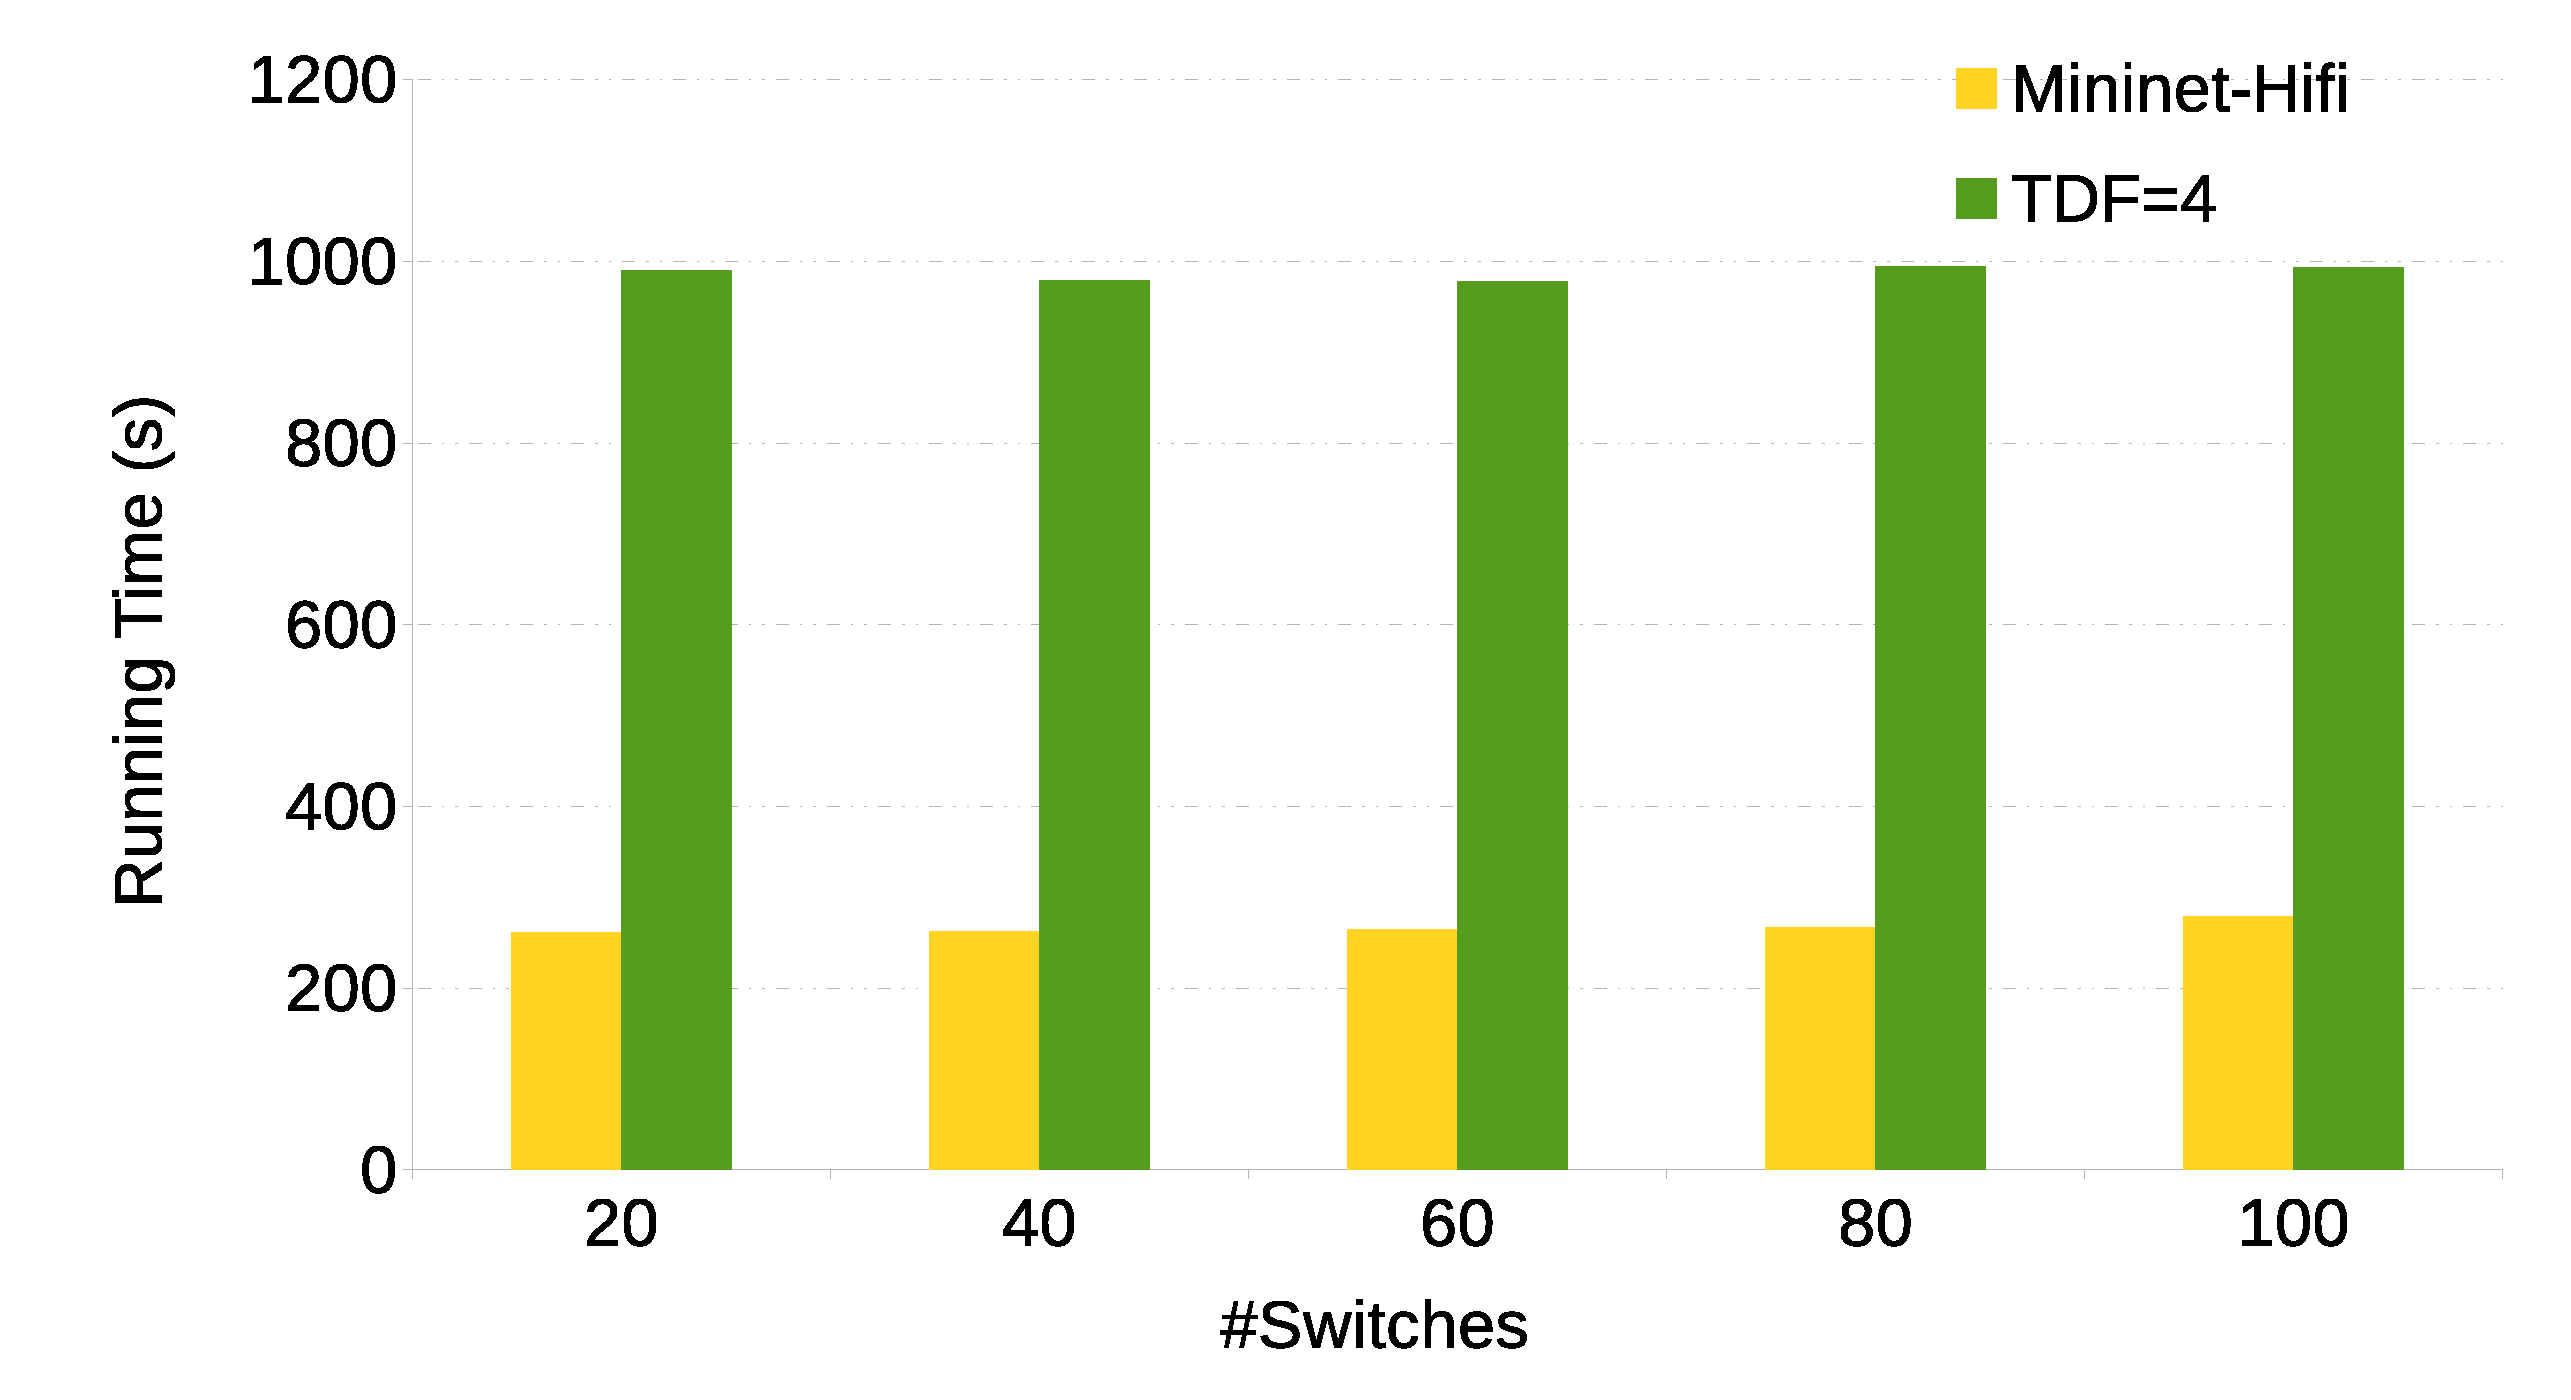
\epsfig{file=VirtualTime/figures/ScaleTime100Sw4GbLink.eps, width=0.45\textwidth}}
    \label{VT:Fig:ScaleTime}}
    \caption{Scalability Evaluation Experimental Results}
\end{figure}

\Subsection{Adaptive TDF Scheduling}
We design a set of emulation experiments consisting of multiple TCP flows to evaluate the adaptive TDF scheduling algorithm.
The network topology has a simple linear structure as shown in Figure~\ref{VT:Fig:LinearTopoExample} and consists of 100 hosts and 99 switches.
All the links are of 100 Mbps bandwidth and 1 ms delay.
We selected 5 non-overlap client-server pairs: \texttt{(h1, h20), (h21, h40), h(41, h60), h(61, h80), (h81, h100)}.
The entire experiment was divided into three phases: (1) initially, transmit flow \texttt{(h1,h20)},
(2) after 50 seconds, transmit all five flows, and (3) after 150 seconds, stop all the transmissions except for flow \texttt{(h1,h20)}.
The goal is to evaluate how our adaptive time dilation scheduler behaves under dynamic emulation workloads with the peak load exceeding Mininet's capability.

We ran the experiments in three cases.
In case 1, TDF was set to 1 (i.e., no virtual time) and the adaptive virtual time scheduling was disabled.
All flows' TCP throughputs measured by \texttt{iperf3} over time are plotted in Figure~\ref{VT:Fig:5FlowsNoVT}. 
In case 2, we enabled the adaptive time dilation management system with TDF initially set to 1,
and conducted the same emulation experiments. Figure~\ref{VT:Fig:5FlowsAdaptiveVT} plots the throughputs of all five flows.
In case 3, we used a fixed TDF ($TDF = 11$) and disabled the adaptive virtual time scheduling.
Results are shown in Figure~\ref{VT:Fig:5FlowsFixedVT}.
We set $TDF=11$ because 11 was the largest value observed in the TDF changing history in case 2.
In addition, the entire trace of the dynamic TDF in case 2 is plotted in Figure~\ref{VT:Fig:HistoryTDF}.
We repeated each experiment for 5 times and observed very similar behaviors.
All the time series reported in Figure~\ref{VT:Fig:Adaptive} were based on the data collected from one run. 

In phase 1, Mininet had sufficient system resources to emulate a single TCP flow \texttt{(h1, h21)}.
Therefore, we observe the close-to-line-rate throughput, i.e., 100 Mbps, in all three cases.
In phase 2, there were five concurrent flows in the network and each case demonstrated different behaviors.
Note that those flows were non-overlap flows because they did not share any links or switches.
Therefore, all five flows should achieve close-to-line-rate throughputs, i.e., 100 Mbps, in physical world applications.
In case 1, the throughputs of all five flows were very unstable as shown in Figure~\ref{VT:Fig:5FlowsNoVT},
which reflected the heavy resource contention in Mininet.
In contrast, in case 3, all five flows have stable, close-to-100-Mbps throughputs because of the virtual time.
In case 2, we observed disturbances in throughput at the beginning of phase 2,
but the five flows quickly converged to the stable close-to-line-rate throughput because the adaptive TDF scheduler managed to compute the optimal TDF value.
The details of TDF adjustment are depicted in Figure~\ref{VT:Fig:HistoryTDF}.
In phase 3, the emulation returned back to a single flow \texttt{(h1, h21)}, and the measured throughputs were accurate in all three cases.
As indicated by Figure~\ref{VT:Fig:HistoryTDF}, our scheduler decreased the TDF value accordingly
in case 2 to save emulation time in phase 3 while still preserving the fidelity.

Table~\ref{VT:Tab:CompareRunTime} summarizes the execution time, the average TDF,
and the rate of execution time in wall clock to the emulation time (200 seconds) of all three cases. 
We can see that case 3 ($TDF = 11$) is around 10 times slower than case 1 ($TDF = 1$) in order to guarantee fidelity.
Our adaptive time dilation scheduler managed to reduce 46\% of the running time as compared to case 3 with little fidelity loss. 

\begin{figure}
    \centering
    \subfigure[TCP Throughput without Virtual Time]{{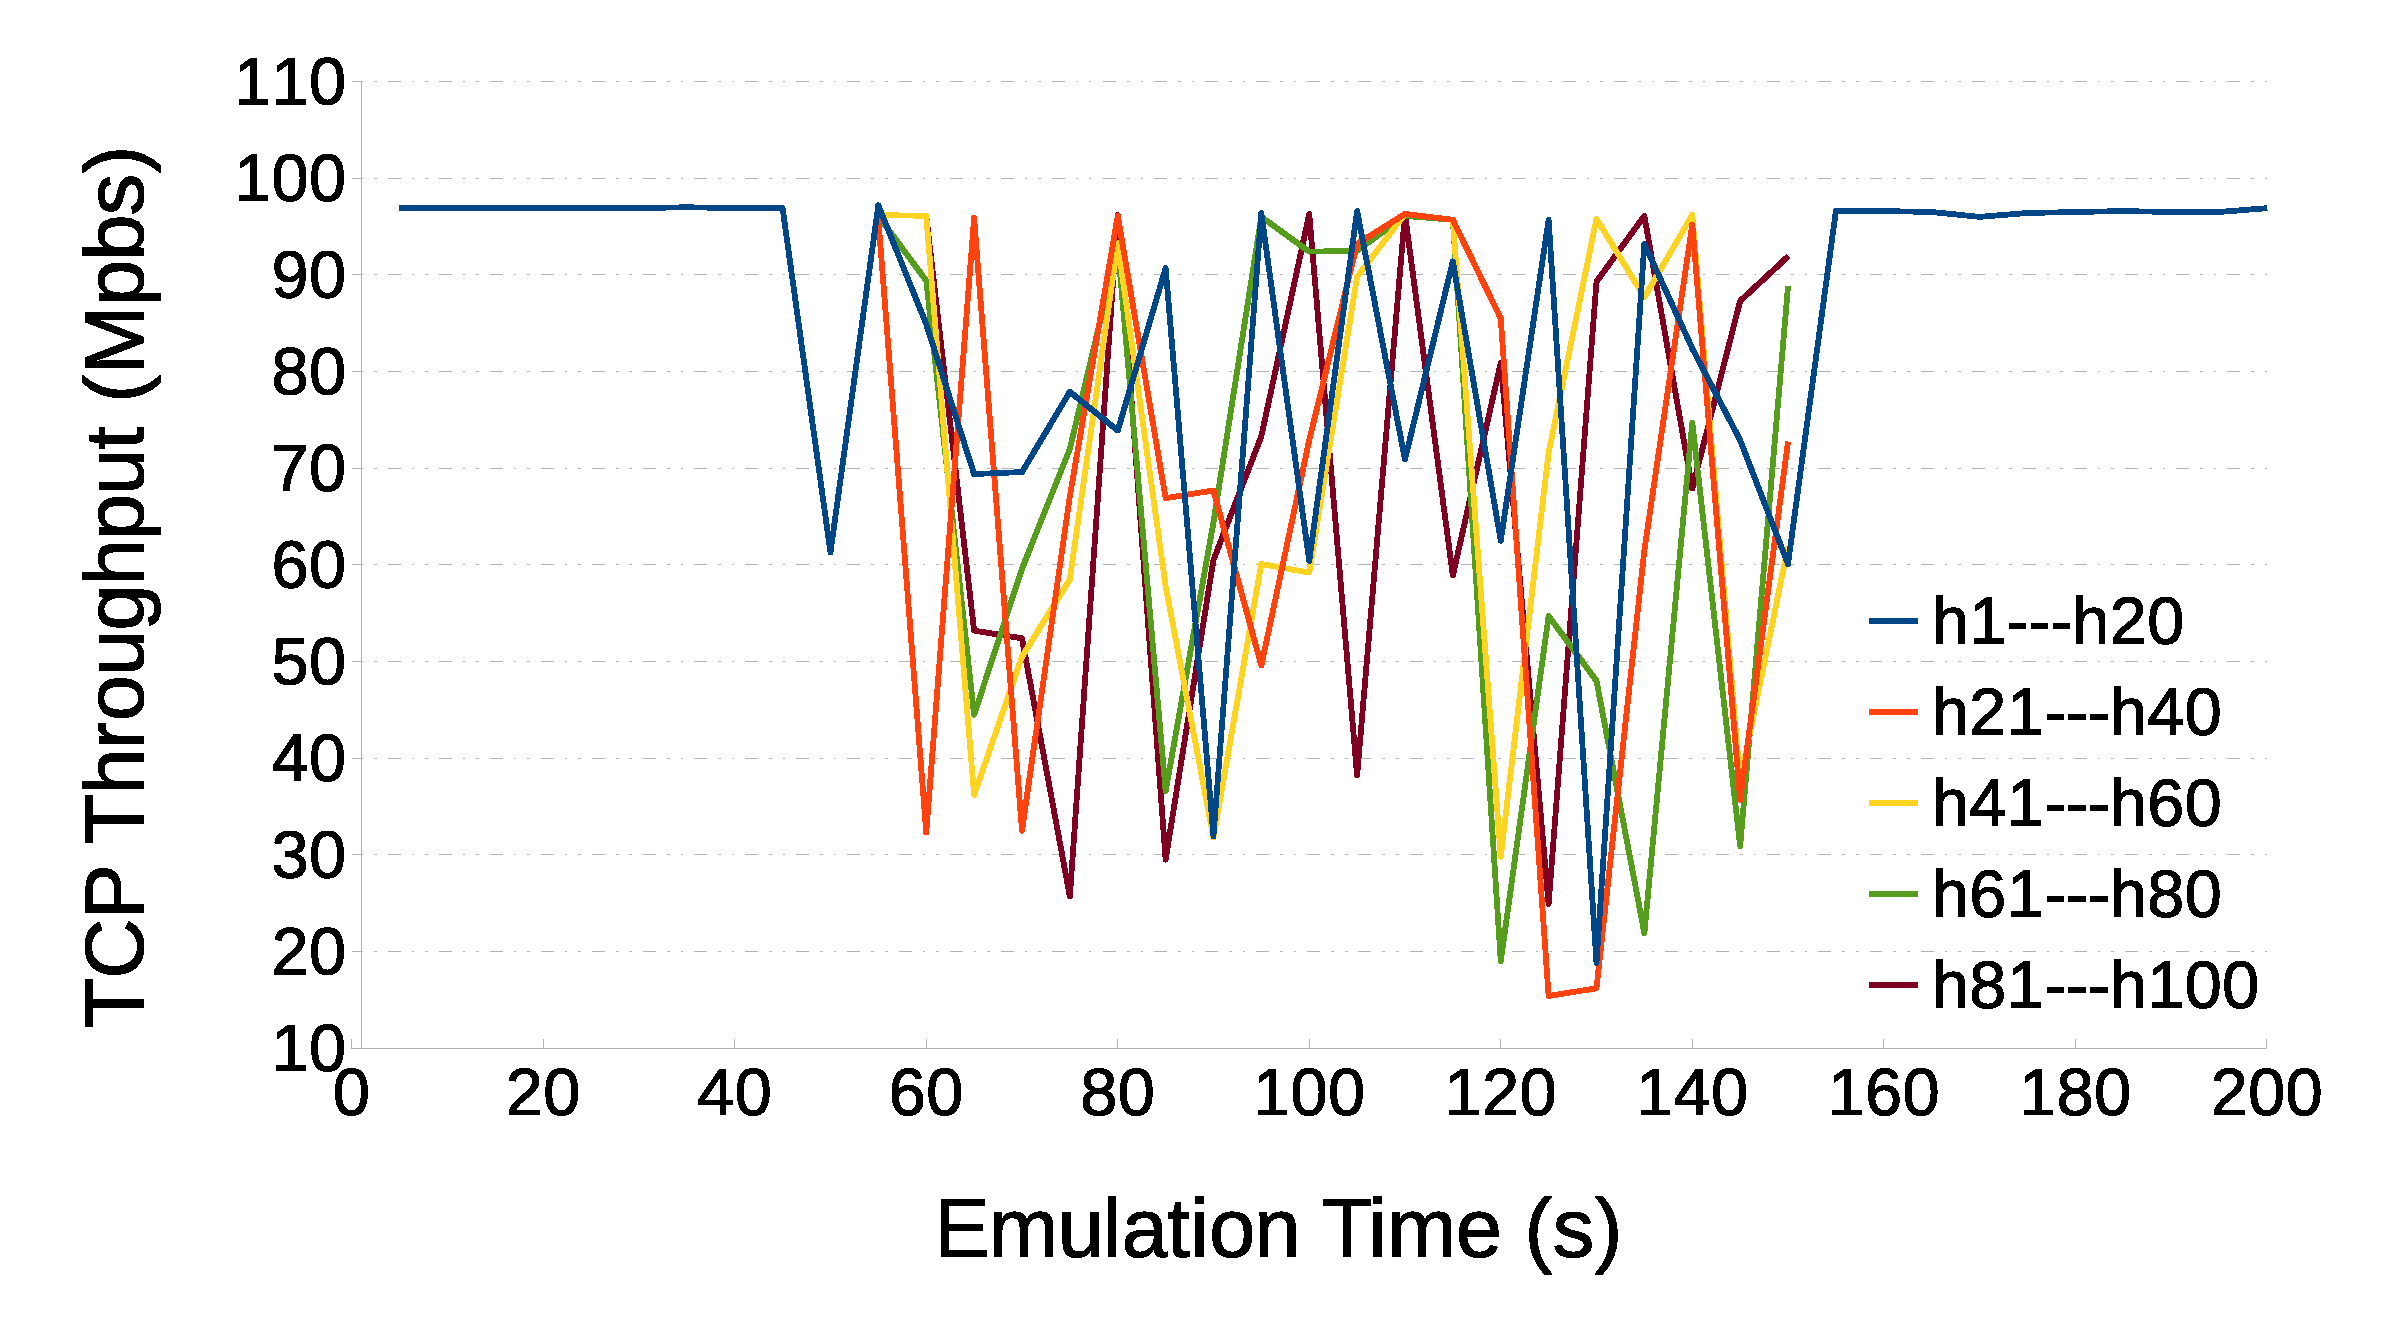
\epsfig{file=VirtualTime/figures/5FlowsNoVT.eps, width=0.45\textwidth}}
    \label{VT:Fig:5FlowsNoVT}}
    \subfigure[TCP Throughput with Adaptive Time Dilation]{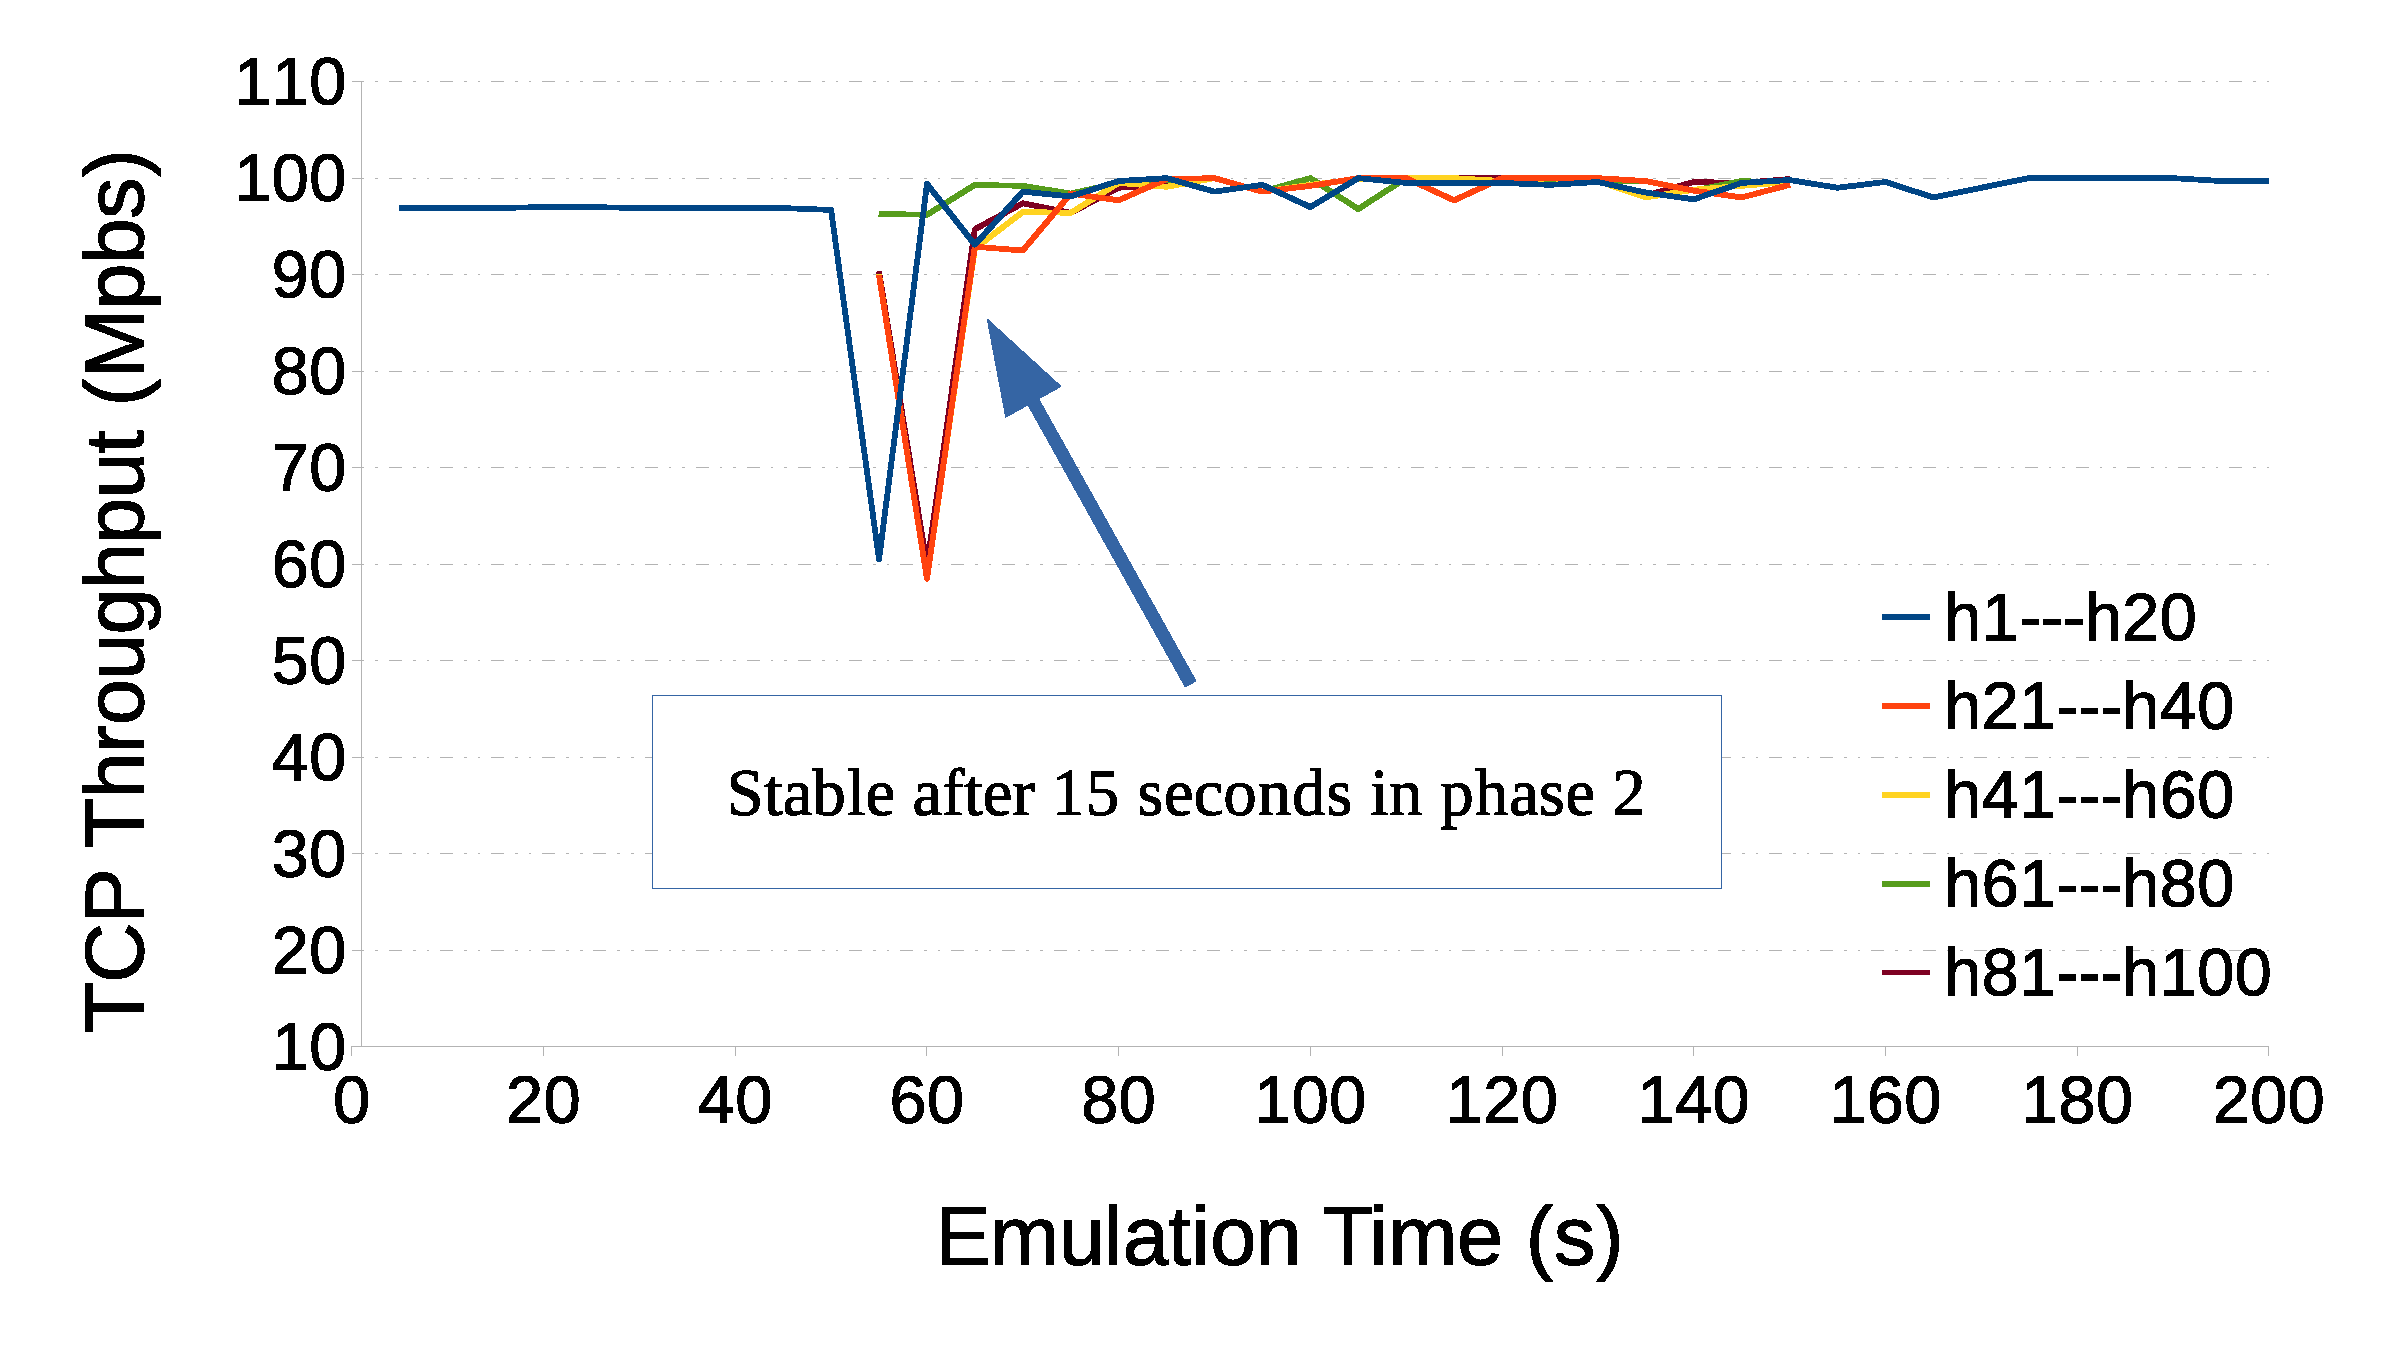
\epsfig{file=VirtualTime/figures/5FlowsAdaptiveVT.eps, width=0.45\textwidth}
    \label{VT:Fig:5FlowsAdaptiveVT}}
    \\
    \subfigure[TCP Throughput with Fixed Time Dilation (11)]{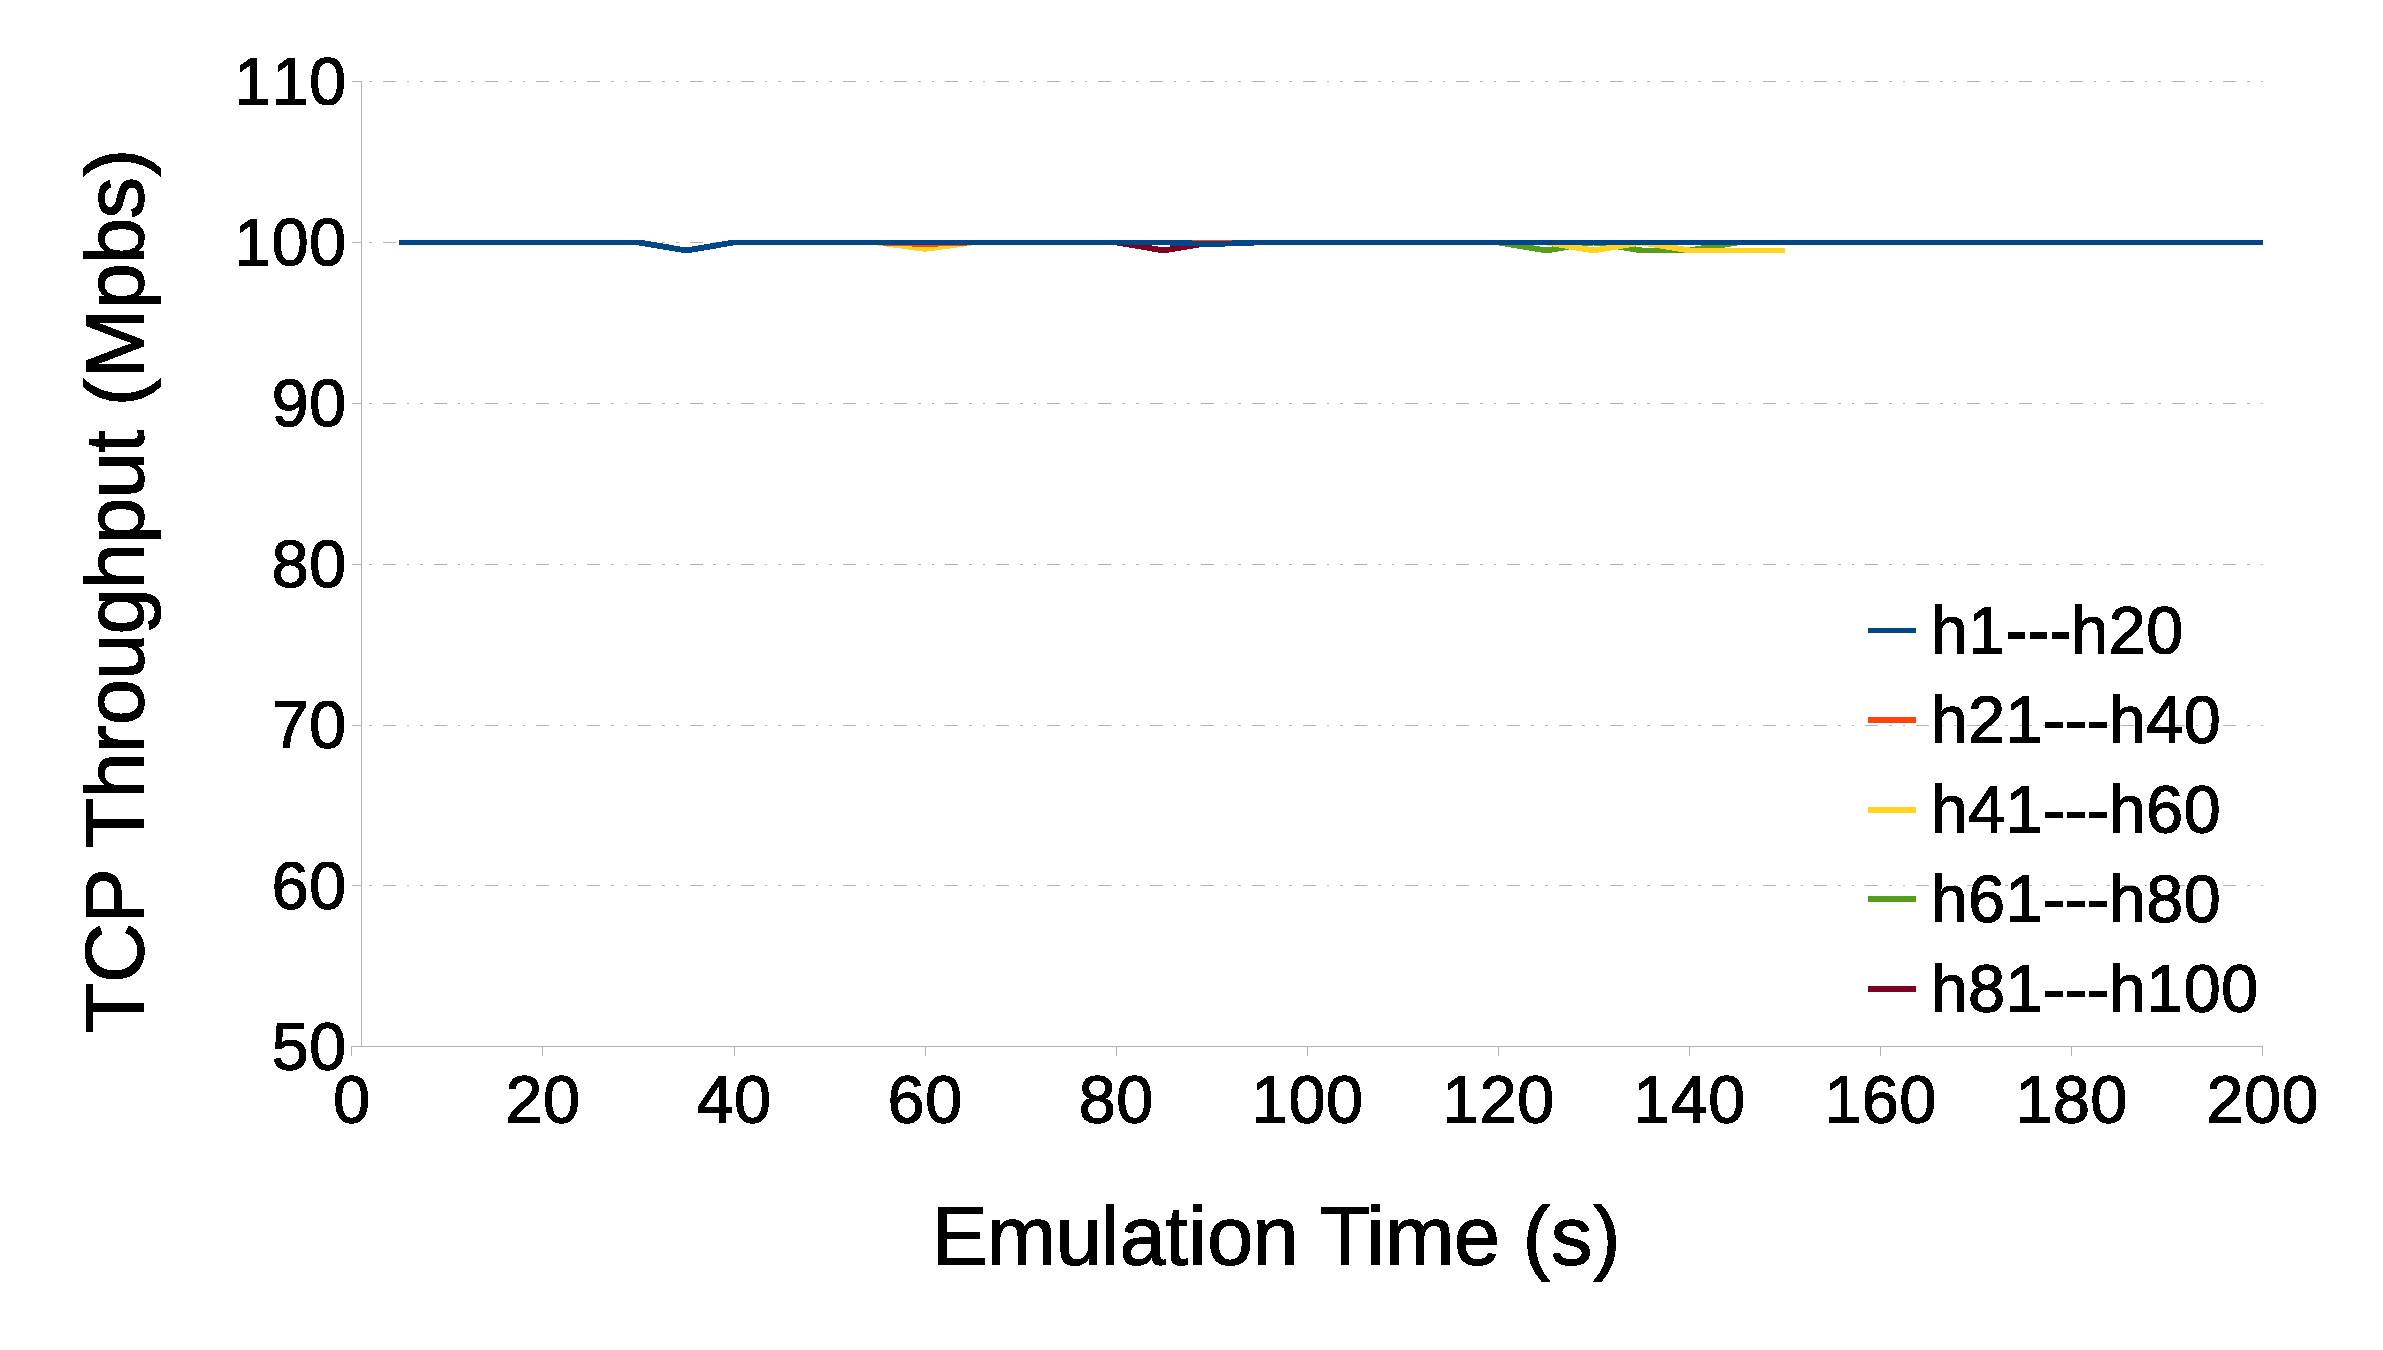
\epsfig{file=VirtualTime/figures/5FlowsFixedVT.eps, width=0.45\textwidth}
    \label{VT:Fig:5FlowsFixedVT}}
    \subfigure[TDF Trace: Adaptive Virtual Time Scheduling]{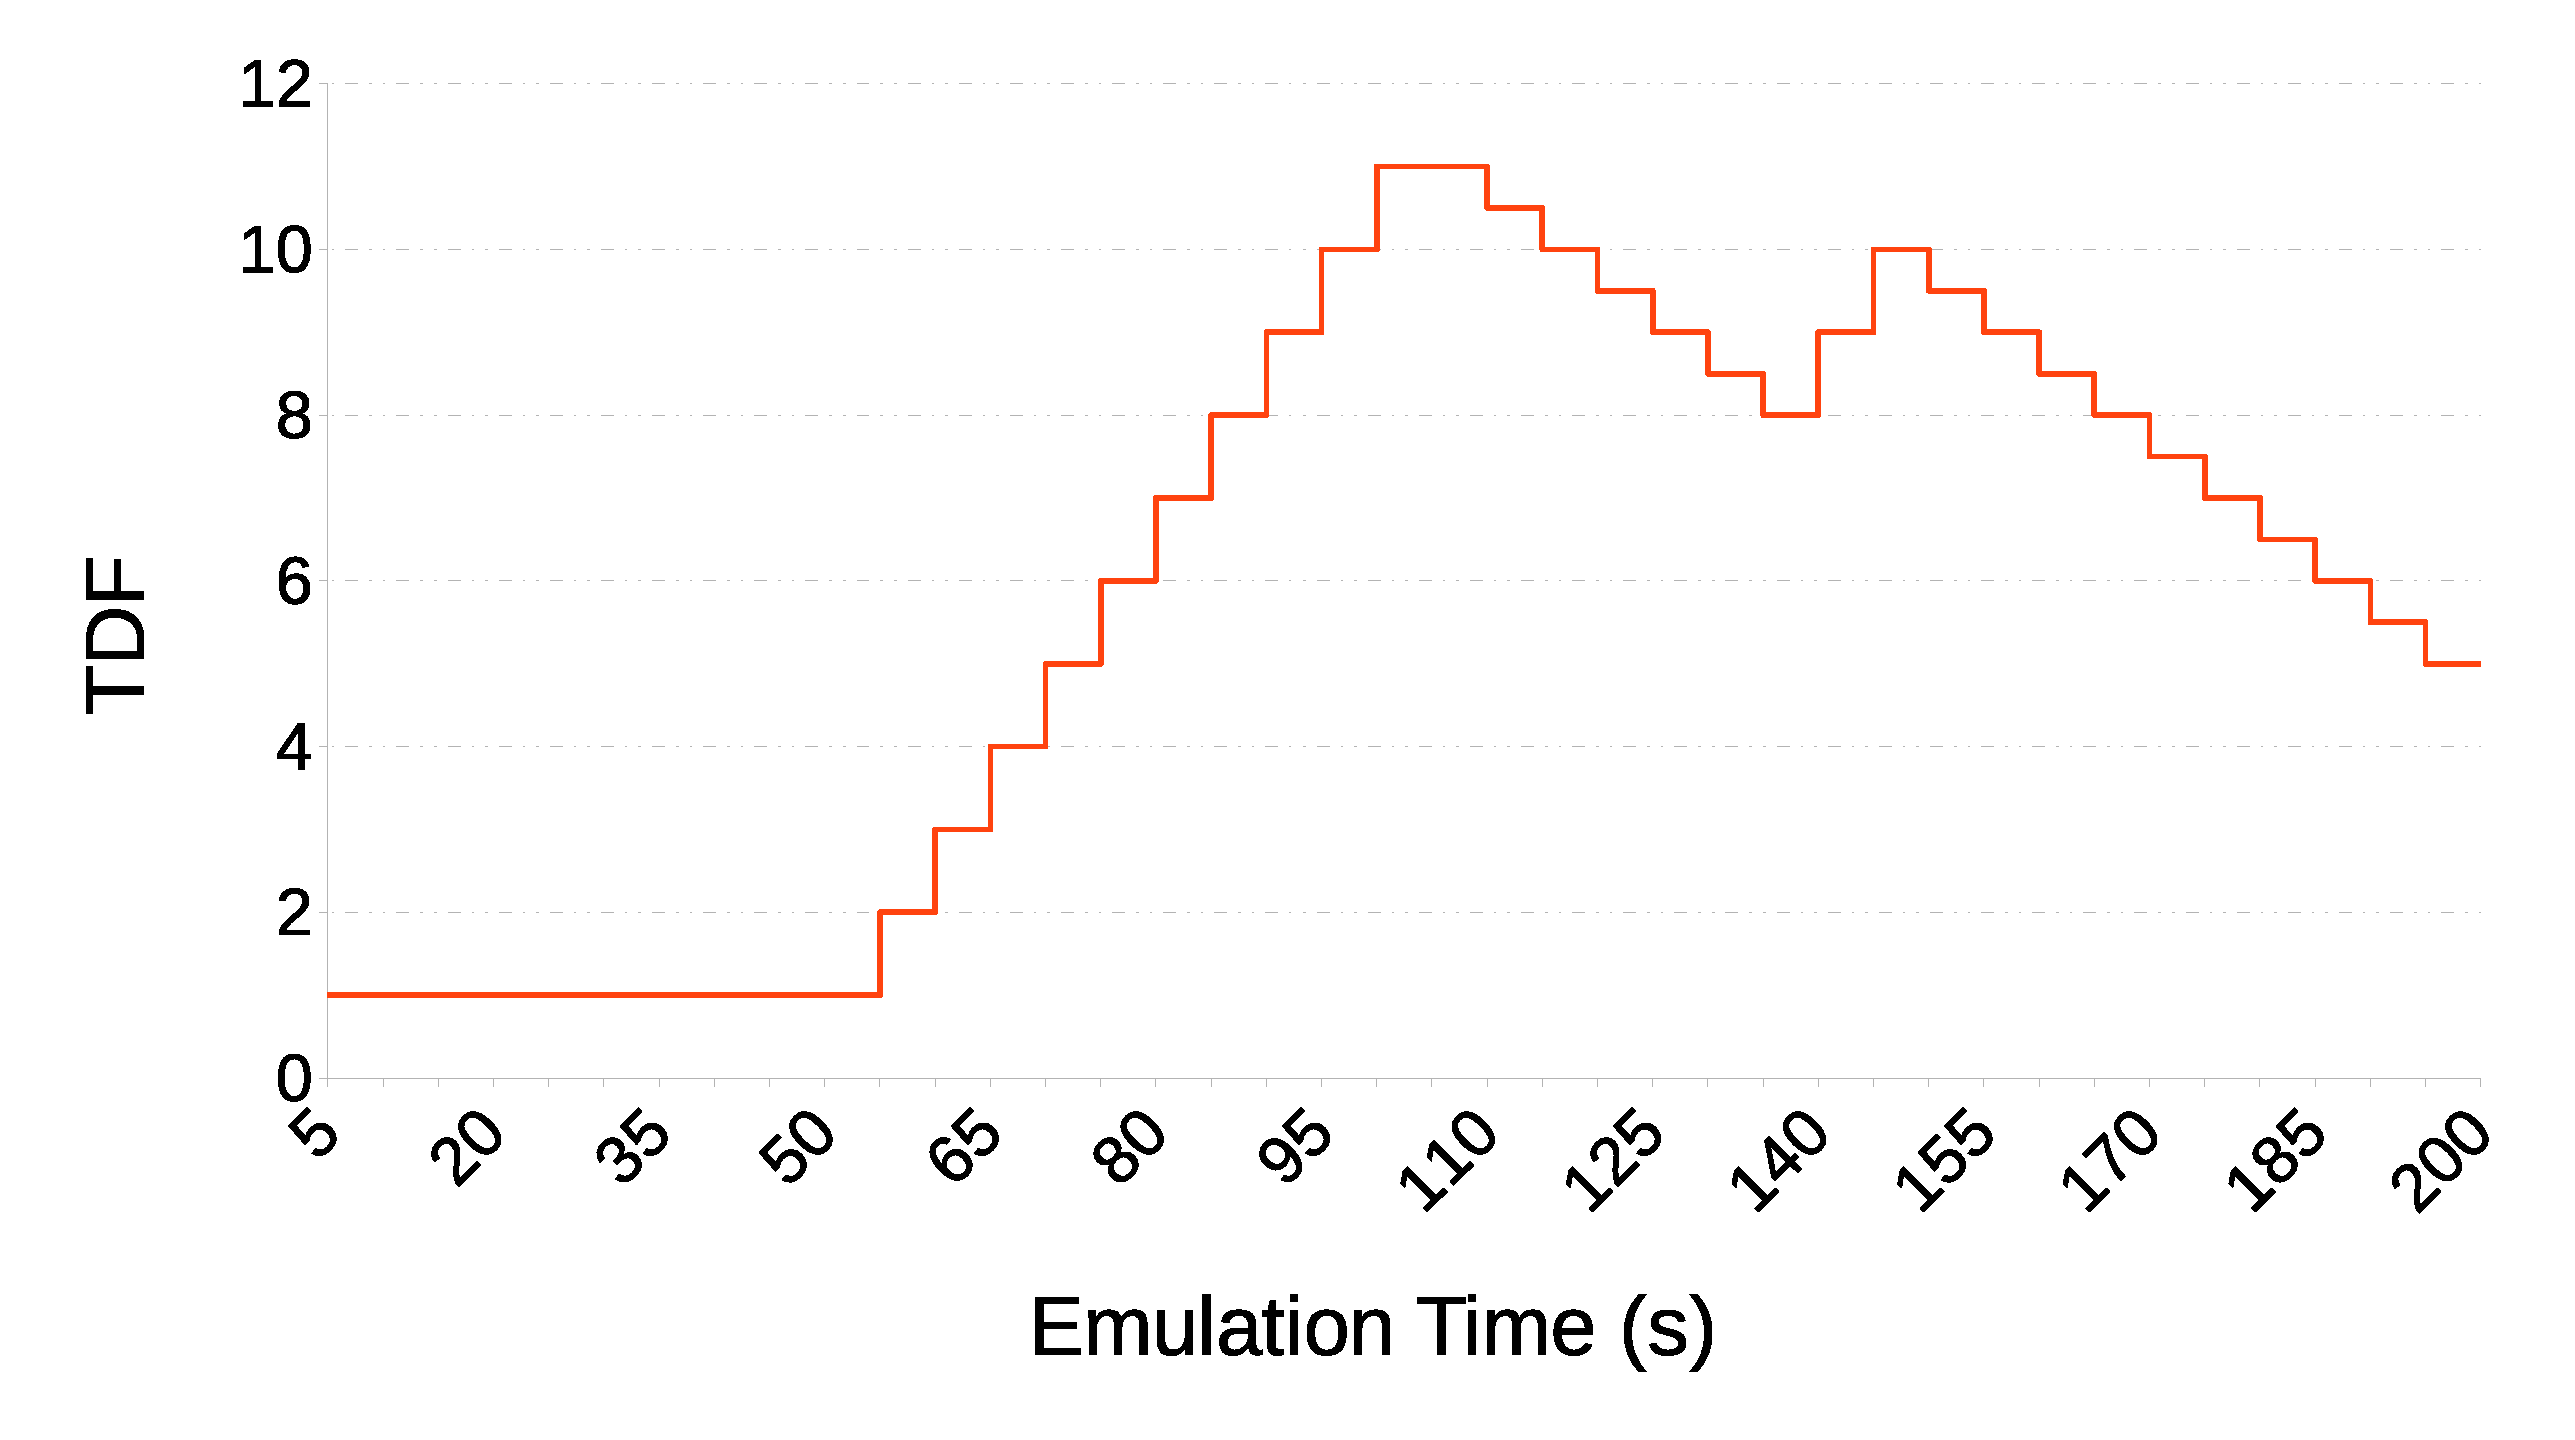
\epsfig{file=VirtualTime/figures/5FlowsHistoryTDF.eps, width=0.45\textwidth}
    \label{VT:Fig:HistoryTDF}}
    \caption{Adaptive Virtual Time Scheduling Evaluation}
    \label{VT:Fig:Adaptive}
\end{figure}

\begin{table*}
    \centering
    \caption{Comparison of Emulation Execution Time}
    \begin{tabular}{c|c|c|c} 
        \hline
        & No Virtual Time & Adaptive Virtual Time & Fixed Virtual Time \\ 
        \hline
        \hline
        Running Time (s)  & 240.730 & 1332.242 & 2434.910 \\ 
        \hline
        Average TDF & 1.000 & 5.900 & 11.000 \\ 
        \hline
        %Slow Down Ratio & 1.204 & 5.534 & 10.115 \\
        Slow Down Ratio & 1.000 & 5.534 & 10.115 \\
        %\hline
        %AVG. CPU\% & 31.968 & 28.287 & 20.376 \\ 
        %\hline
        %STDEV. CPU\% & 10.915 & 7.175 & 4.173 \\ 
        \hline
    \end{tabular}
    \label{VT:Tab:CompareRunTime}
\end{table*}

\Subsection{System Overhead}
Our virtual time system introduces overhead with the following two reasons:
(1) the computation cost in Algorithm~\ref{VT:Alg:VirtualTimeKeeping} and
(2) the pauses of emulation when changing containers' TDFs.
We measured both types of overhead and report the results in Table~\ref{VT:Tab:Overhead}.

First, we invoked both non-dilated and dilated \texttt{gettimeofday} 10,000,000 times from a user space application.
The average overhead for one dilated \texttt{gettimeofday} is 0.013 microseconds.
We then used \texttt{strace} to count the number of invocations for \texttt{gettimeofday} in a 60-second \texttt{iperf3} run on both the server and the client.
The total overhead is 18,145 microseconds after tracing 1,397,829 calls, which is about 0.03\% of the 60-second experiment. 
Actually, \texttt{iperf3} intensively invokes \texttt{gettimeofday},
because its timer is designed to exhaustively inquiry the OS time.
The overhead amount will be even less for many other network applications.
We also repeatedly changed a process's TDF 10,000,000 times using another test program.
The average pause time was 0.063 microseconds, which is reasonably small.
Since the number of TDF changes issued by the current adaptive TDF scheduling algorithm
is a few orders of magnitude less than the number of calls to \texttt{gettimeofday}
(e.g., only 14 TDF transitions occurred per host over the period of 1,332 seconds in the earlier adaptive TDF experiment), that overhead is also negligible.

\begin{table*}
    \centering
    \caption{Lightweight Virtual Time System: Overhead of System Calls}
    \begin{tabular}{c|c|c|c}
        \hline
        & No Virtual Time & Virtual Time & Avg Overhead / System Call \\%& Overhead Rate in E  \\ 
        \hline
        \hline
        \texttt{gettimeofday}  & 0.0532 $\mu$s & 0.0661 $\mu$s & 0.0129 $\mu$s\\% & $3.0 \times 10^{-4}$\\ 
        \hline
        \texttt{setTDF} & 0  & 0.0628 $\mu$s & 0.0628 $\mu$s\\% & $3.65\times 10^{-9}$ \\ 
        \hline
    \end{tabular}
    \label{VT:Tab:Overhead}
\end{table*}



\Section{Case Study: Limitation of ECMP Routing}
\label{VT:Sec:CaseStudy}

Network emulation testbeds are widely used to test and evaluate designs of network applications and
protocols with the goal of discovering design limitations and implementation faults before the real system deployment.
In this section, we present a case study to demonstrate how our virtual-time-enabled Mininet has been utilized to
reproduce and validate the limitations of the equal-cost multi-path (ECMP) routing strategy in a data center network.

Many modern data center networks employ multi-rooted hierarchical tree topologies,
and therefore ECMP-based protocols~\cite{ECMP} are commonly used in data center networks for load-balancing traffic over multiple paths.
When an ECMP-enabled switch has multiple next-hops on the best paths to a single destination,
it selects the forwarding path by performing a modulo-N hash over the selected fields of a packet's header to ensure per-flow consistency.
The key limitation of ECMP is that the communication bottleneck would occur when several large and
long-lived flows collide on their hash and being forwarded to the same output port~\cite{Hedera}. 
We borrowed the experiment scenario on a physical testbed described in~\cite{Hedera},
and created a set of emulation experiments in Mininet to demonstrate the limitation of ECMP.
We built a fat-tree topology in Mininet as shown in Figure~\ref{VT:Fig:FattreeTopoExample},
and generated stride-style traffic patterns. Note that stride($i$) means that a host with index $x$ sends to the host with index $(x + i)$ mod $n$,
where $n$ is the number of hosts~\cite{Hedera}. 
The hash-based ECMP mechanism is provided by the RipL-POX SDN controller~\cite{RipLPox}.
The Mininet code was developed with reference to~\cite{ReproNetReserch}.
In all the following experiments, we set up 8 sender-receiver pairs transmitting stride-pattern traffic flows using step 1 and 4.
Figure~\ref{VT:Fig:FattreeTopoExampleStride1} shows the worst-case collision of 2 flows, distinguished by color, when stride step is 1;
while in Figure~\ref{VT:Fig:FattreeTopoExampleStride4}, we see that 2 TCP flows will cause a lot of collision between core layer and aggregate layer,
which is very common case.

\begin{figure}[ht]
    \centering
    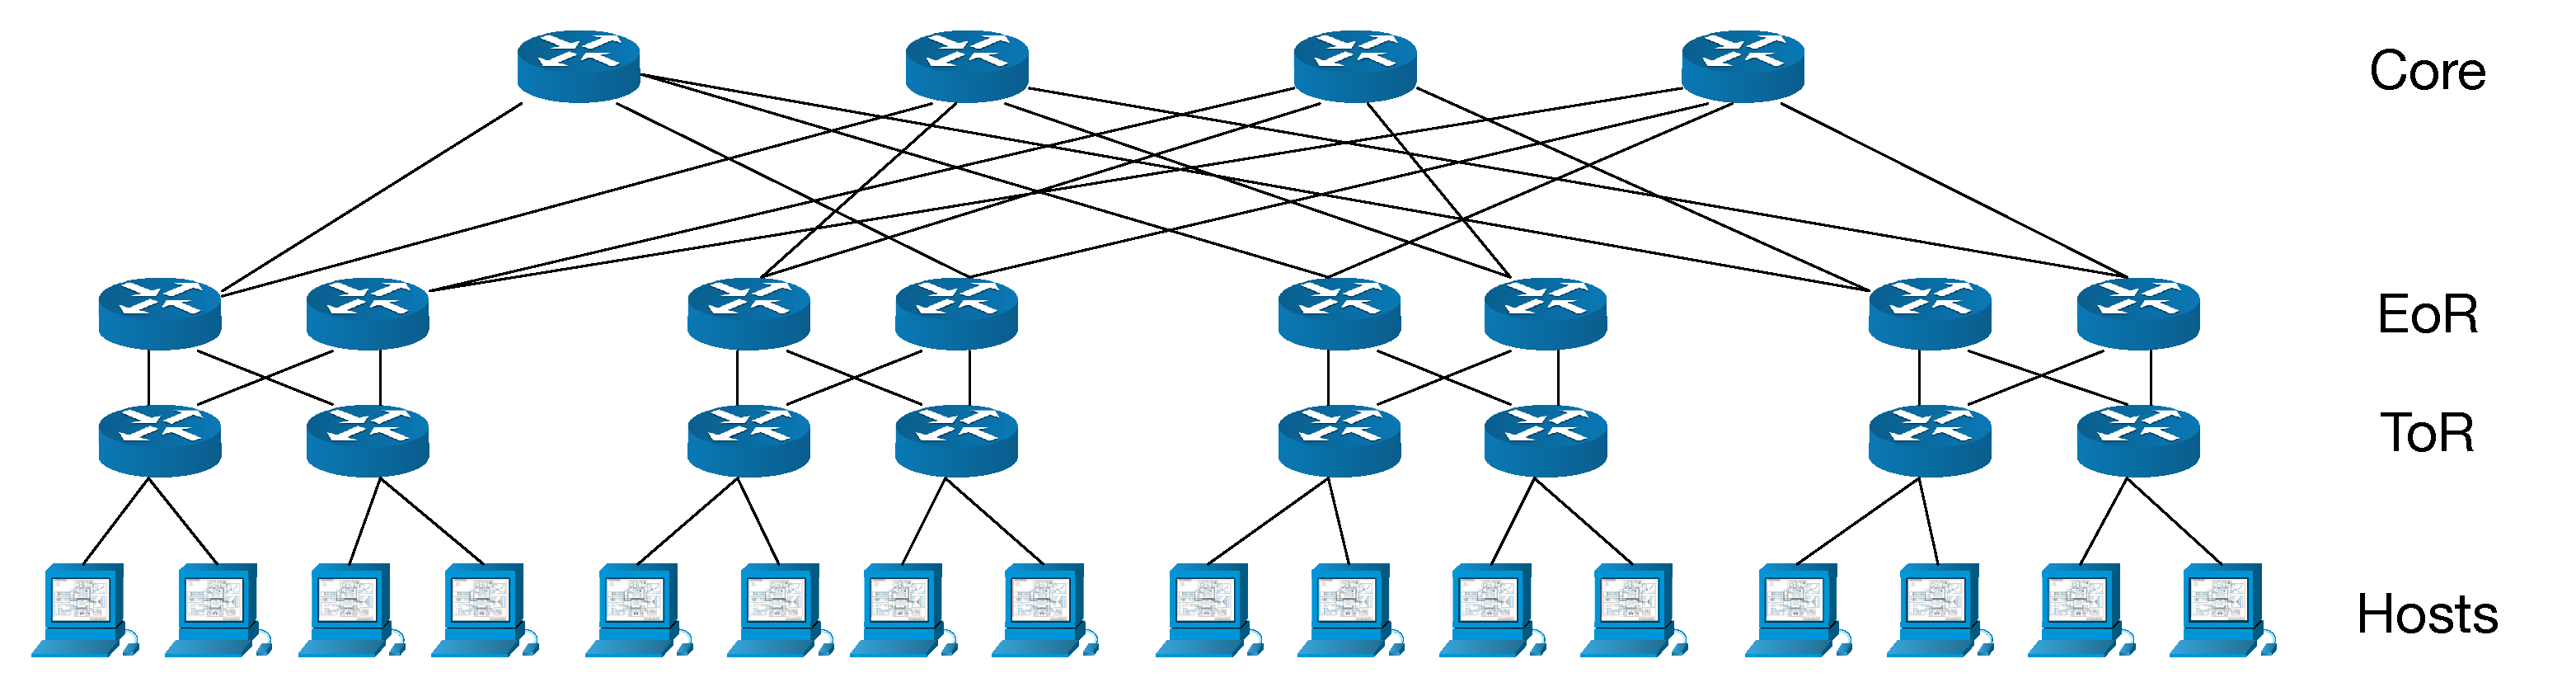
\includegraphics[width=0.8\textwidth]{VirtualTime/figures/TopoFatTreeExample.eps}
    \caption{A Fat-Tree Data Center Network with Degree-4}
    \label{VT:Fig:FattreeTopoExample}
\end{figure}

\begin{figure}[ht]
    \centering
    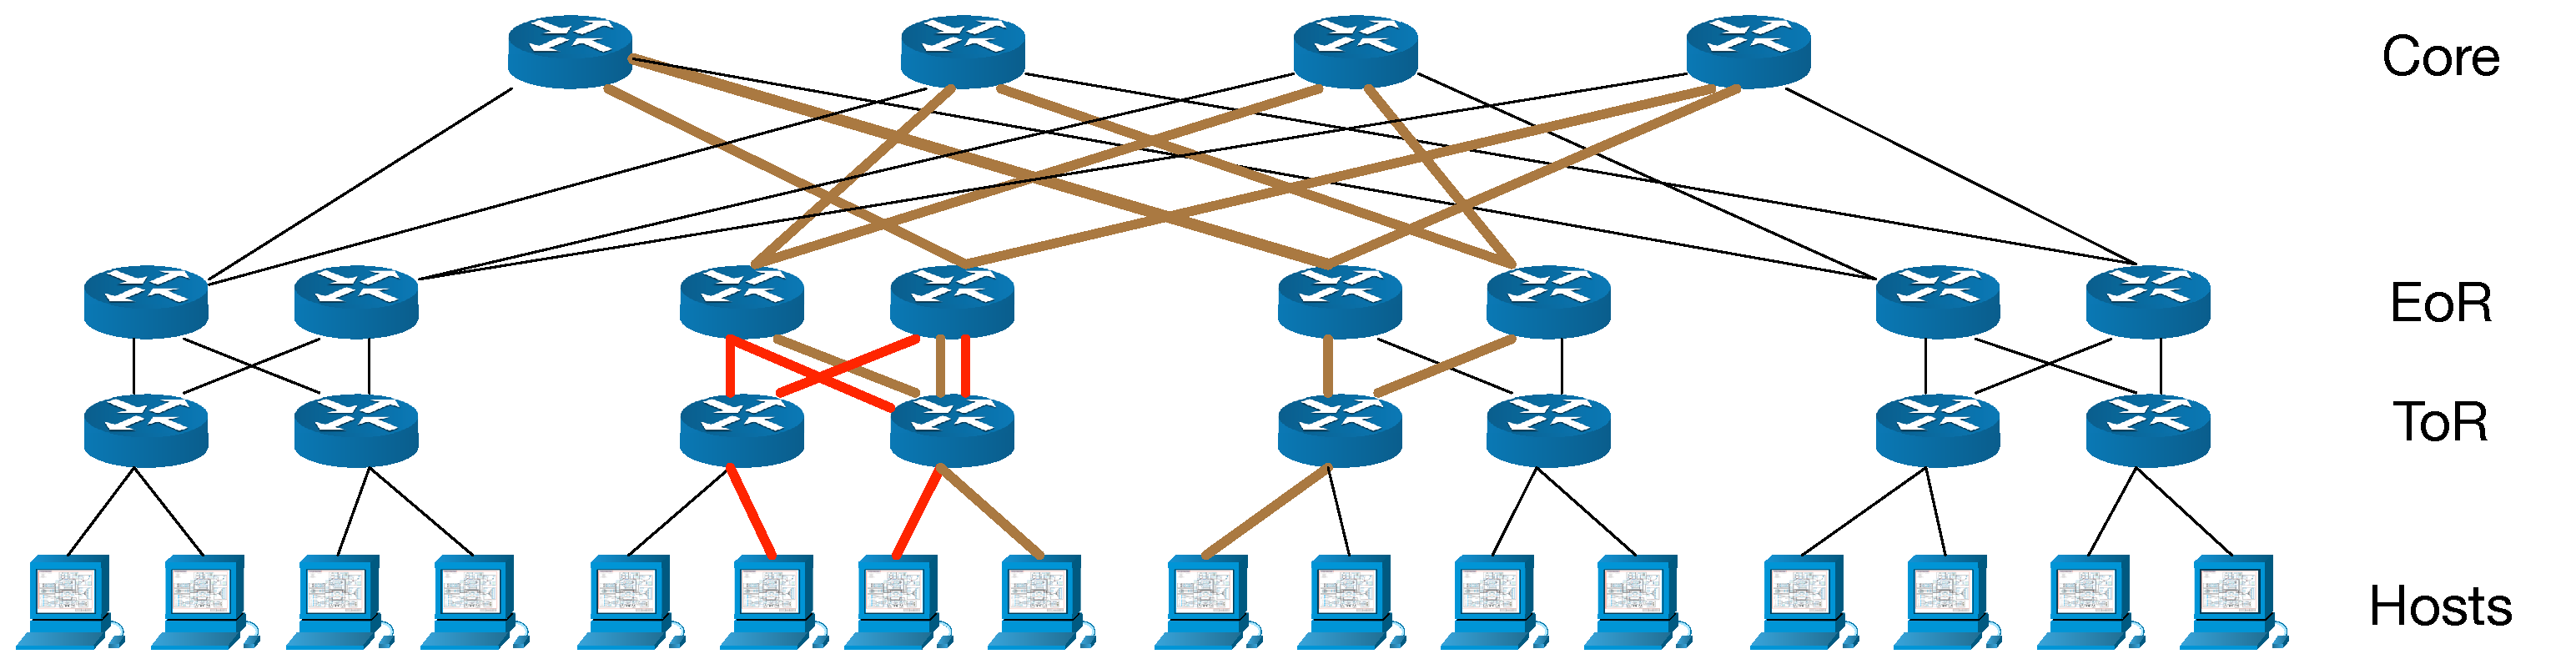
\includegraphics[width=0.8\textwidth]{VirtualTime/figures/TopoFatTreeExampleStride1.eps}
    \caption{Worst-case TCP Flows with Stride Step 1}
    \label{VT:Fig:FattreeTopoExampleStride1}
\end{figure}

\begin{figure}[ht]
    \centering
    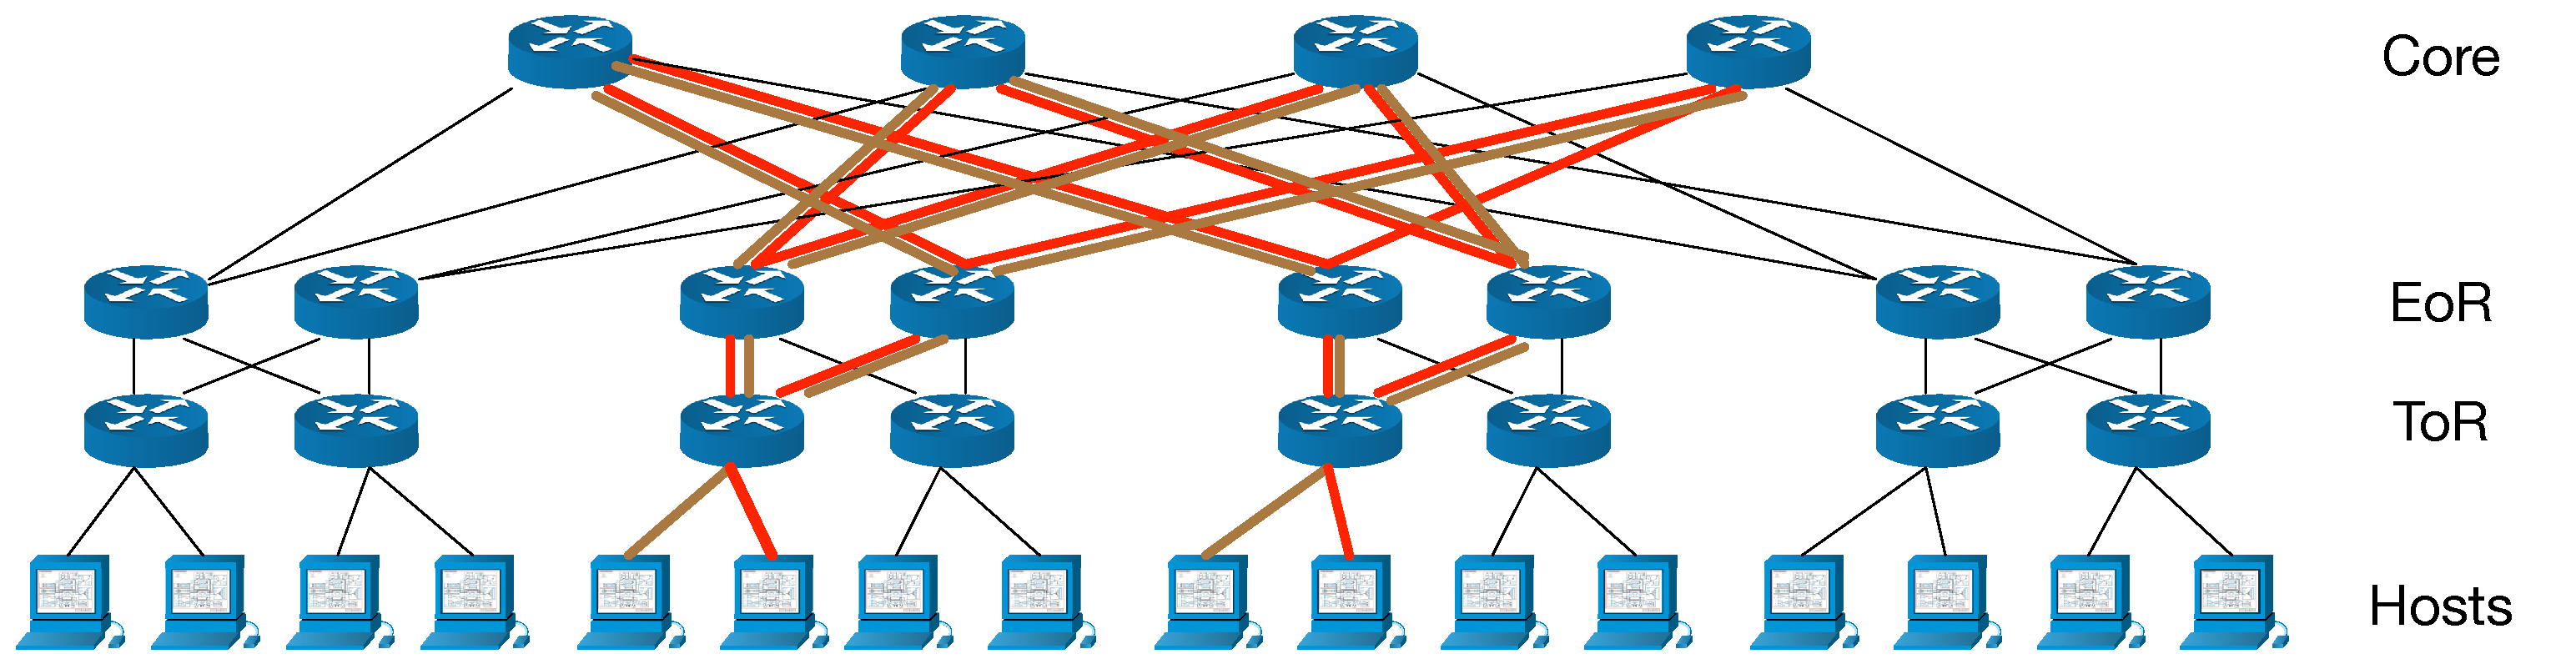
\includegraphics[width=0.8\textwidth]{VirtualTime/figures/TopoFatTreeExampleStride4.eps}
    \caption{Common case TCP Flows with Stride Step 4}
    \label{VT:Fig:FattreeTopoExampleStride4}
\end{figure}

We first set all the link bandwidth (switch-to-switch and switch-to-host) to 100 Mbps,
and conducted each experiment over three independent runs.
The average throughput of 8 TCP flows was plotted in Figure~\ref{VT:Fig:FatTreeAvgBw100M},
and each individual flow's throughput (24 in total) was plotted in Figure~\ref{VT:Fig:FatTreeIndividualBw100M}.
The limitation of ECMP presented in~\cite{Hedera} was clearly observed.
When many conflicting flows occurred with stride-4 flow patterns,
the average throughput in the fat-tree network dramatically fell below 30 Mbps with up to 75\% throughput drop.
As shown in Figure~\ref{VT:Fig:FatTreeIndividualBw100M}, every flow's throughput was largely
affected by the hash collision limitation of ECMP in the stride-4 scenario.

\begin{figure}[ht]
    \centering
    \subfigure[Average TCP Flow Throughput]{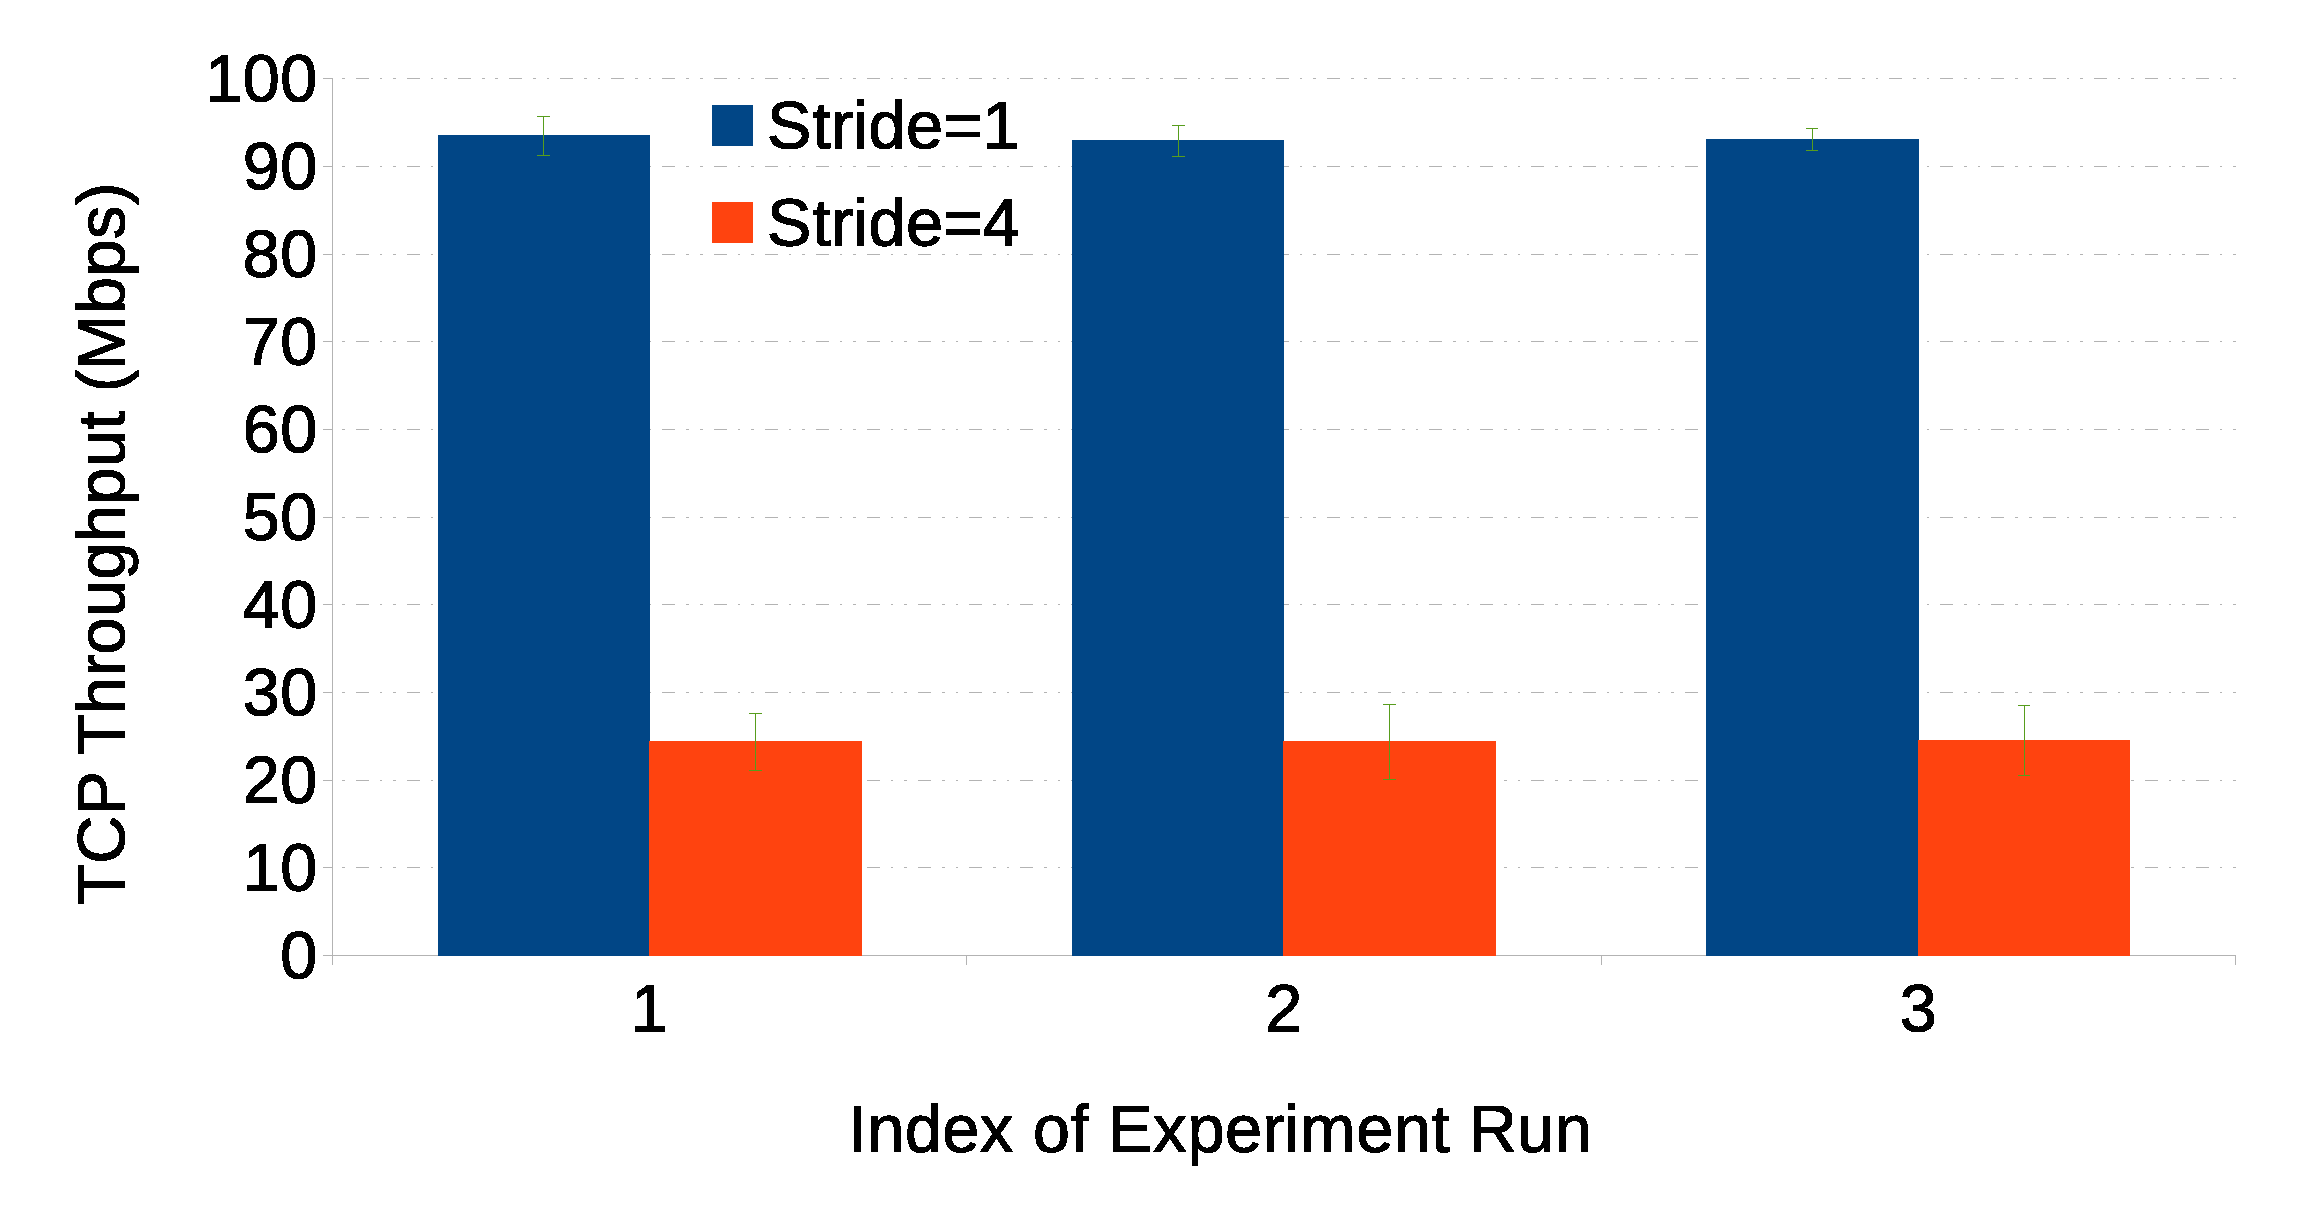
\epsfig{file=VirtualTime/figures/FattreeAvgAggBw100M.eps, width=0.45\textwidth}
    \label{VT:Fig:FatTreeAvgBw100M}}
    \subfigure[Throughput of Individual TCP Flow]{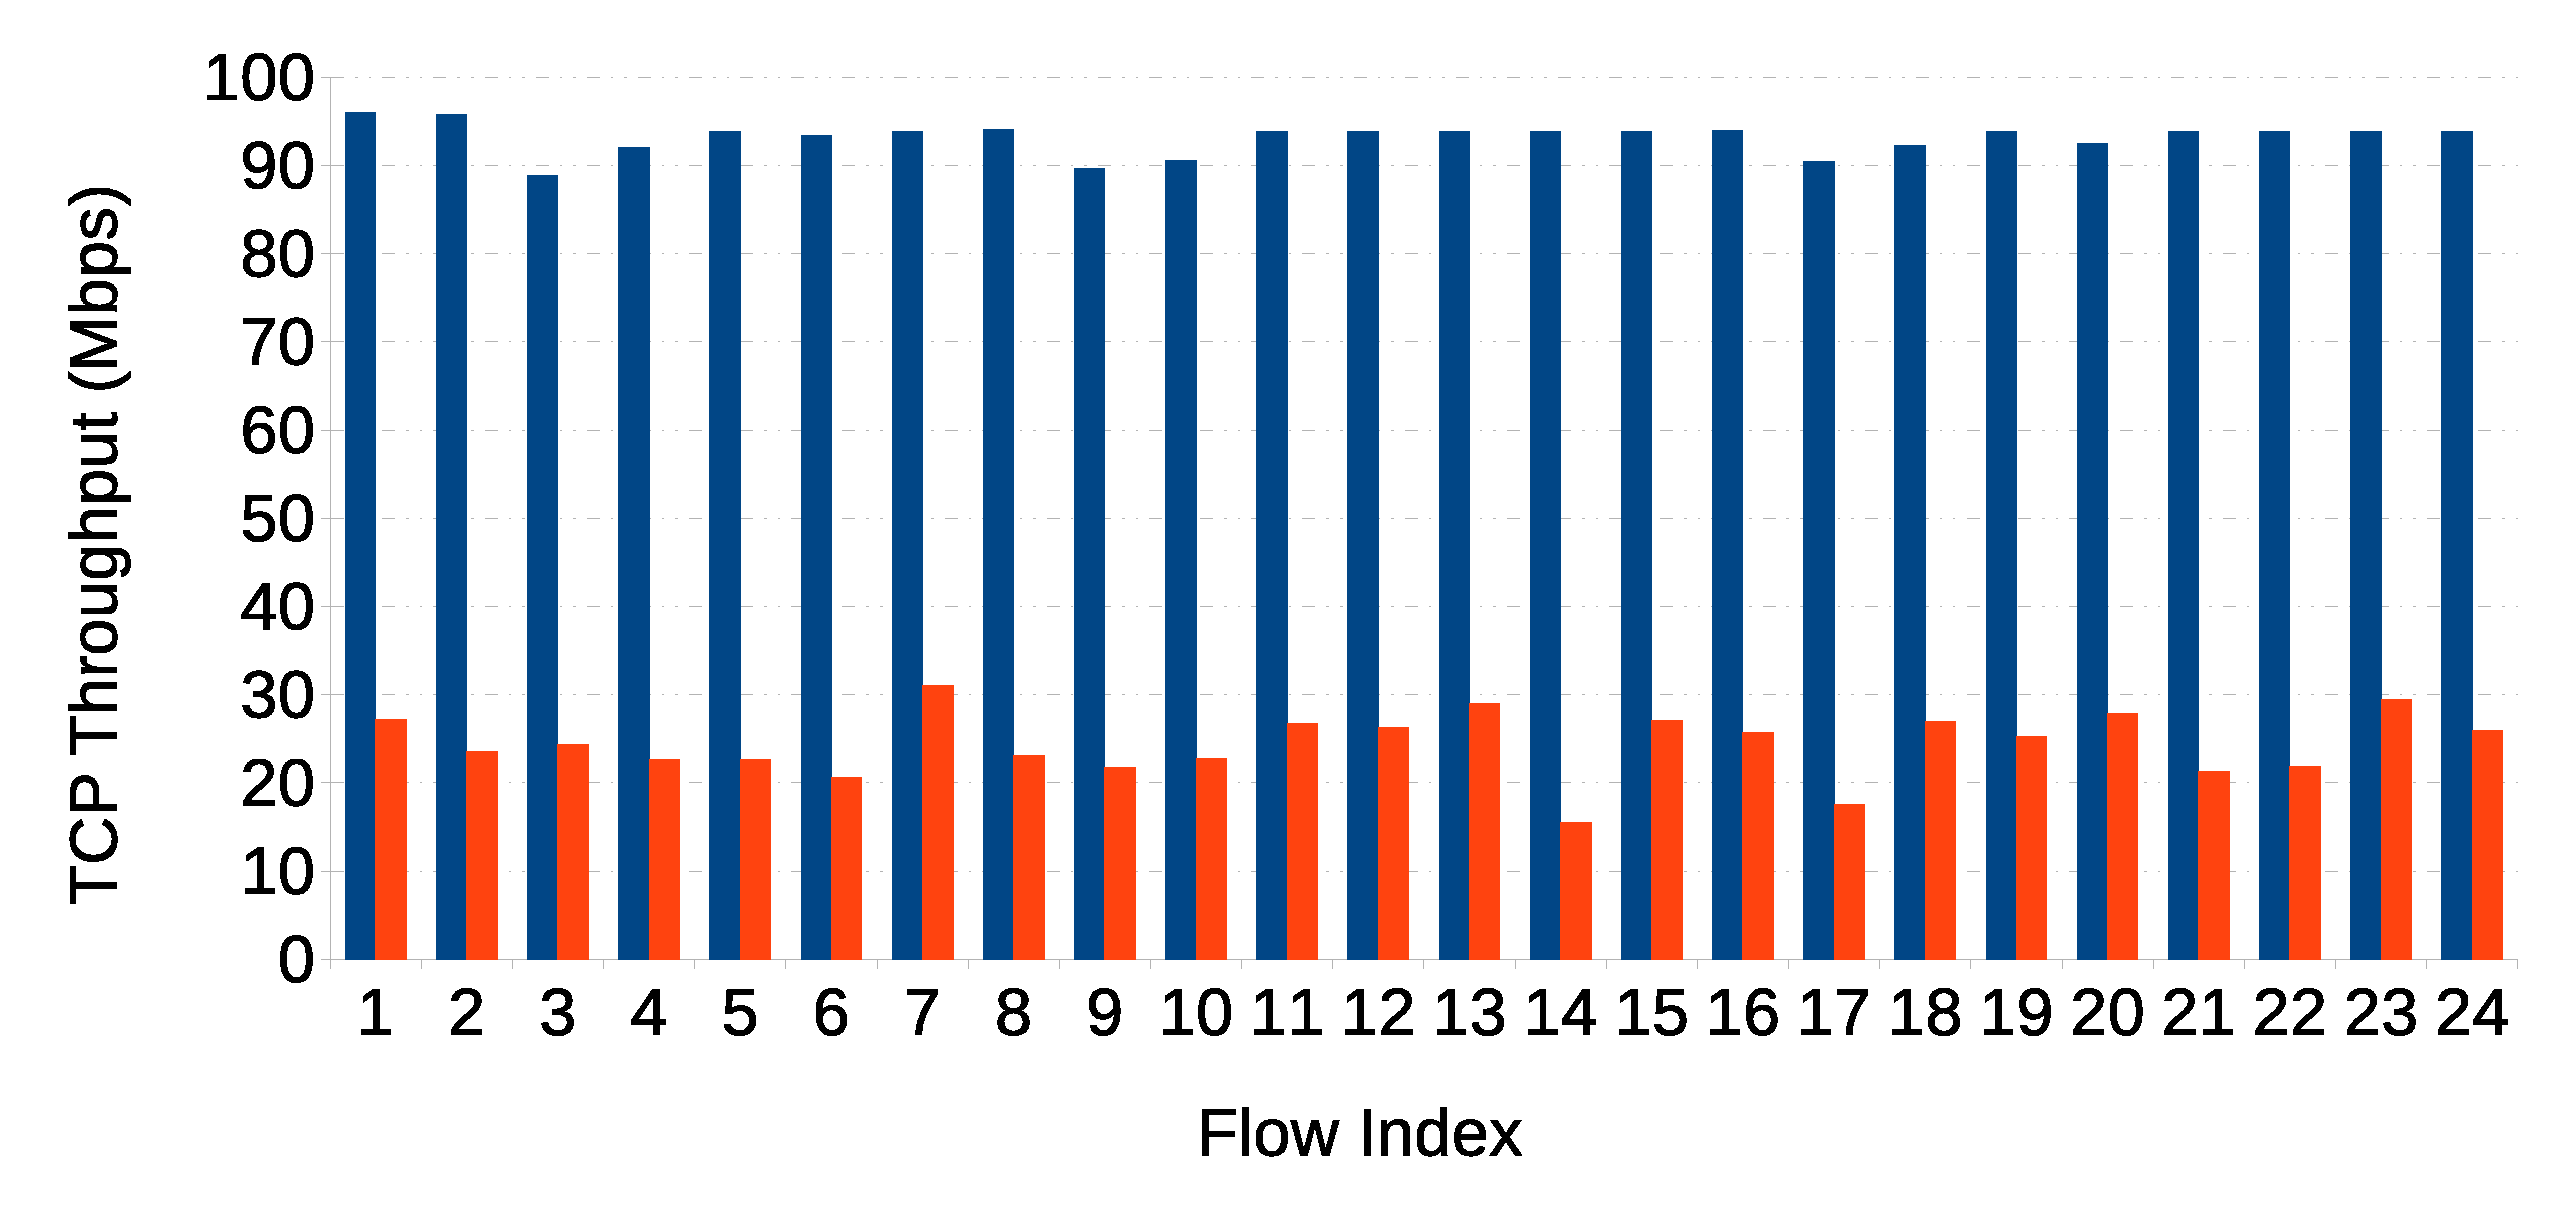
\epsfig{file=VirtualTime/figures/FattreeFlowDistBw100M.eps, width=0.45\textwidth}
    \label{VT:Fig:FatTreeIndividualBw100M}}
    \caption[Emulate ECMP with Low Link Bandwidth]{Mininet Emulation Results: ECMP Limitation in a Fat-tree-based Data Center Network with 100 Mbps Link Bandwidth}
\end{figure}

However, the link bandwidth configuration in the previous experiments are not realistic.
As early as in 2009, links connecting edge hosts to top of rack switches (ToR), ToR to edge of rank switches (EoR),
and EoR to Core switches in a data center had been already above gigabit,
in particular, 10 Gbps switch-to-switch links and 1 Gbps host-to-switch links~\cite{ScaleEffDCN}.
Can Mininet still show us the limitation of ECMP with such high link bandwidth?
If not, can virtual time help to overcome the issue?
Using the same configurations except that links were set to 10 Gbps,
we re-ran the experiments in Mininet without virtual time ($TDF=1$) and with virtual time ($TDF = 4$).
We plotted the average flow throughput in Figure~\ref{VT:Fig:FatTreeAvgBw10G} and
individual flow throughput in Figure~\ref{VT:Fig:FatTreeIndividualBw10G}.

\begin{figure}[ht]
    \centering
    \subfigure[Average TCP Flow Throughput]{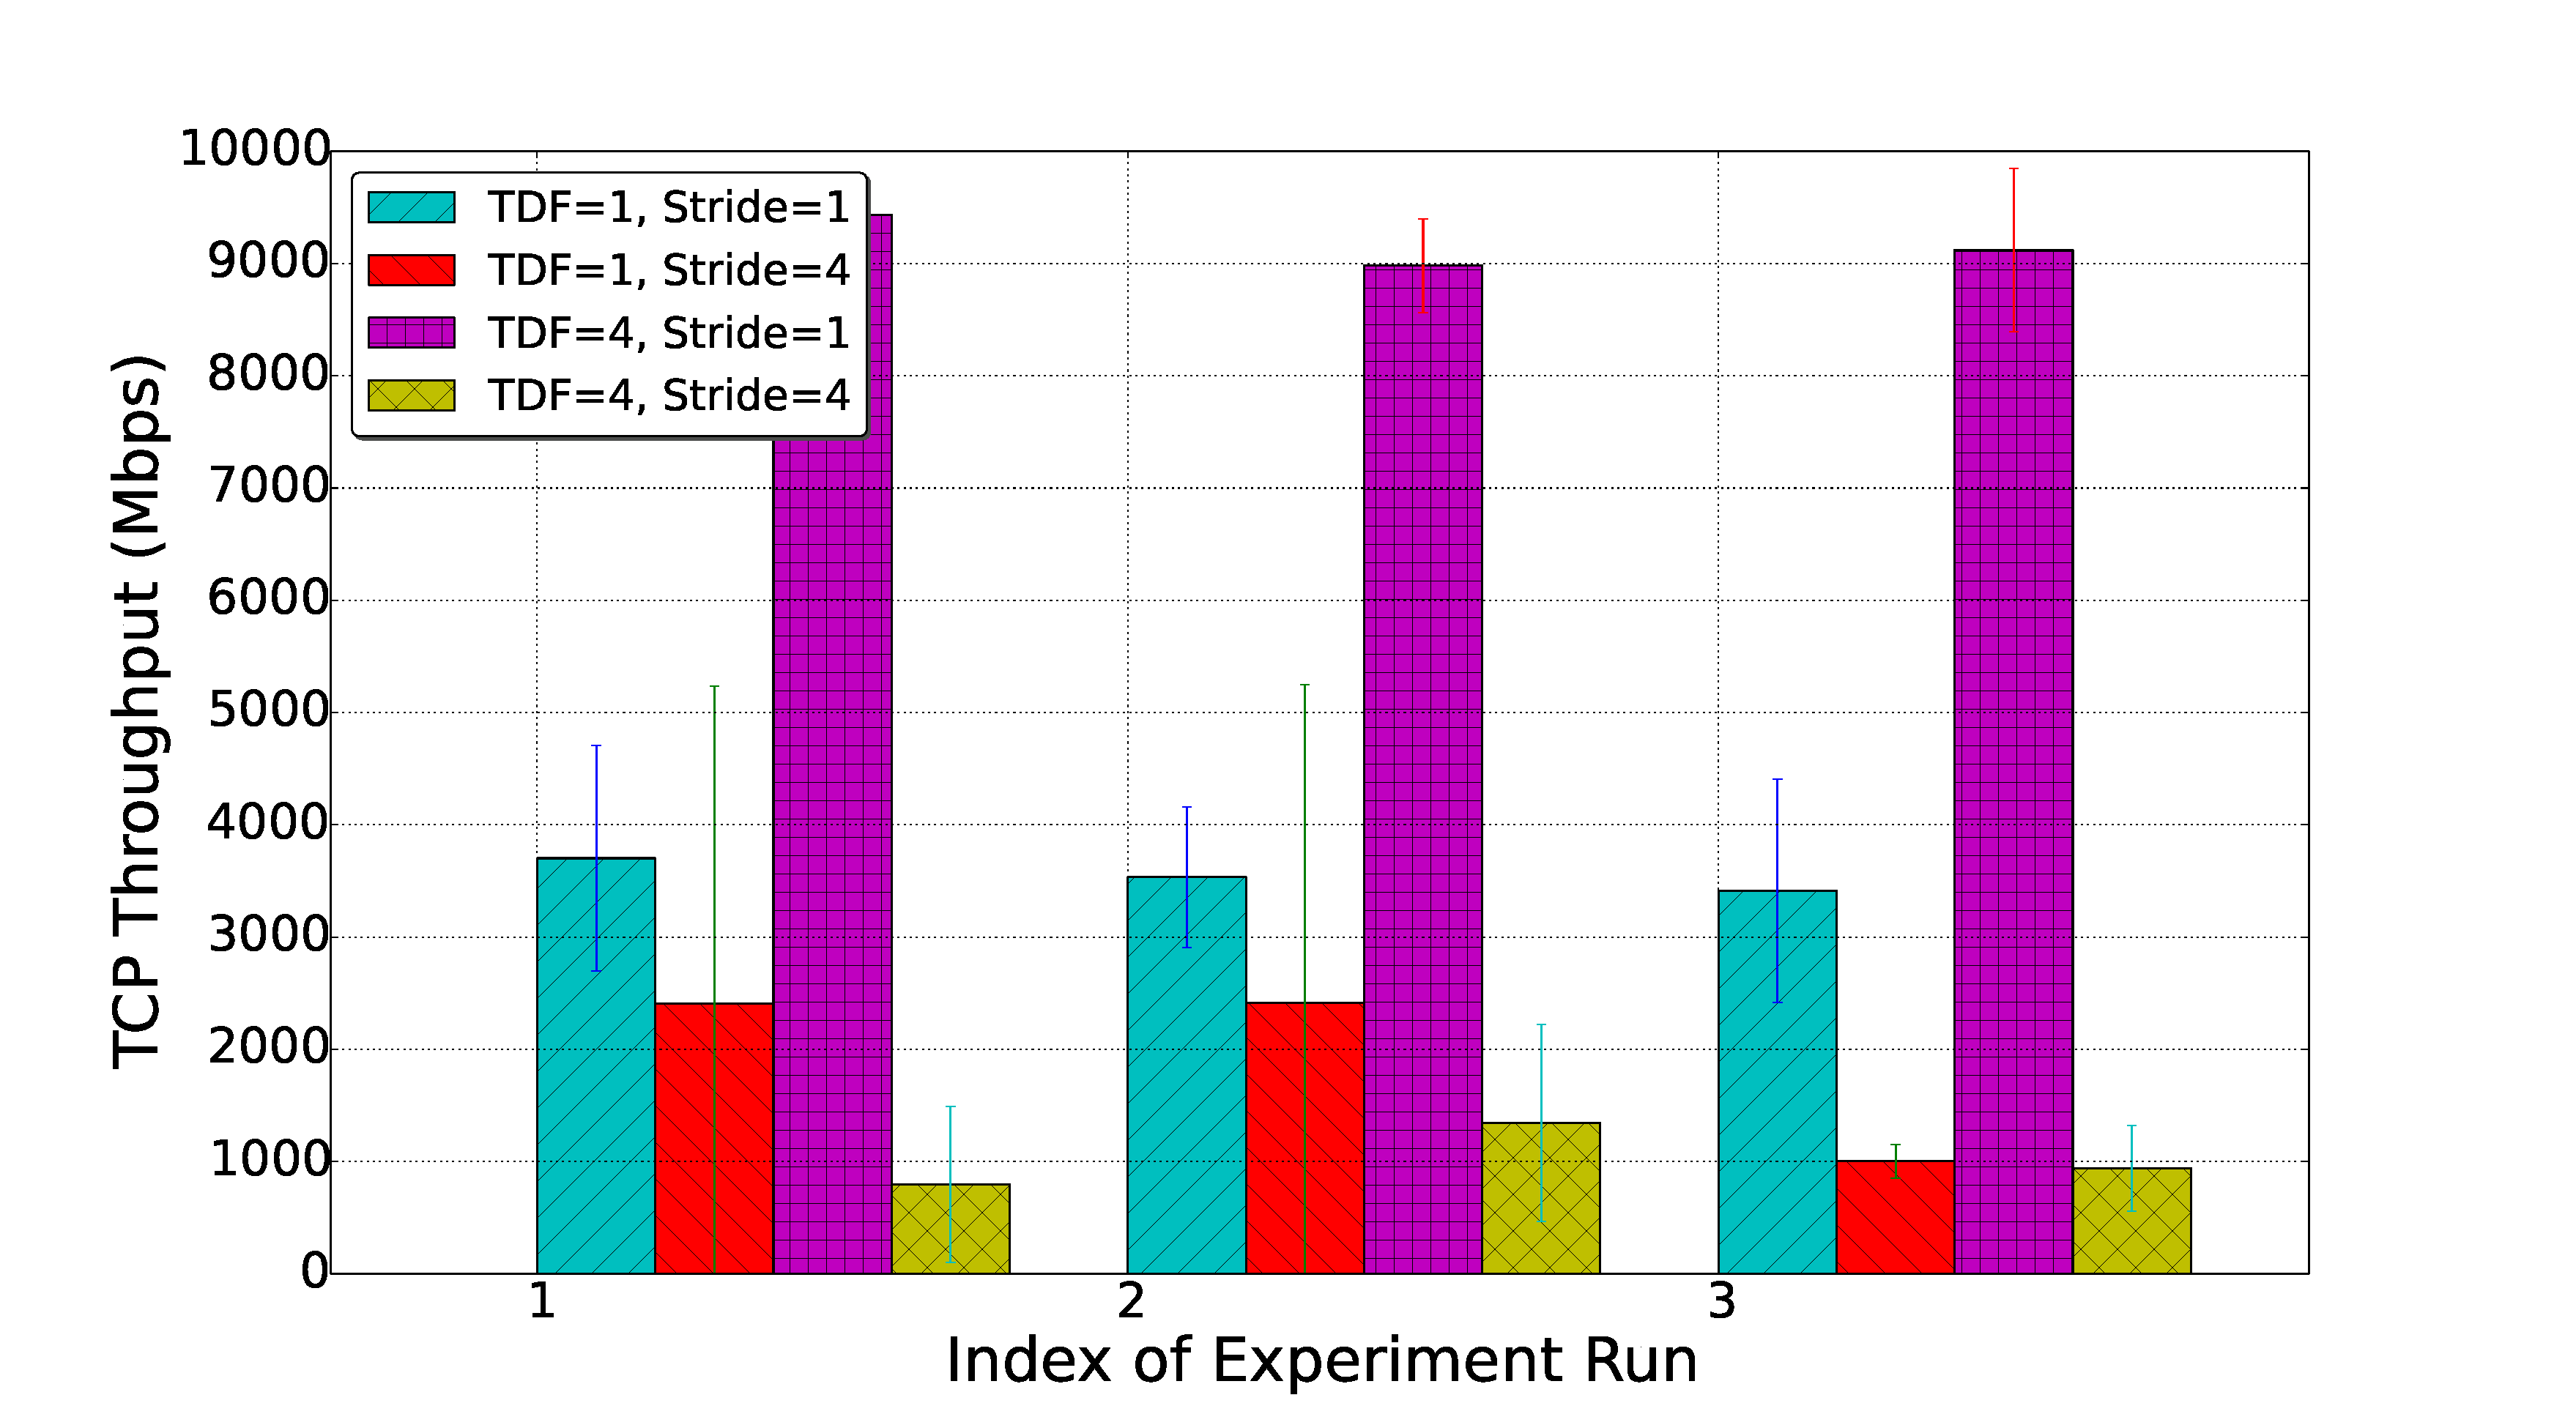
\epsfig{file=VirtualTime/figures/FattreeAvgAggBw10G.eps, width=0.45\textwidth}
    \label{VT:Fig:FatTreeAvgBw10G}}
    \subfigure[Throughput of Individual TCP Flow]{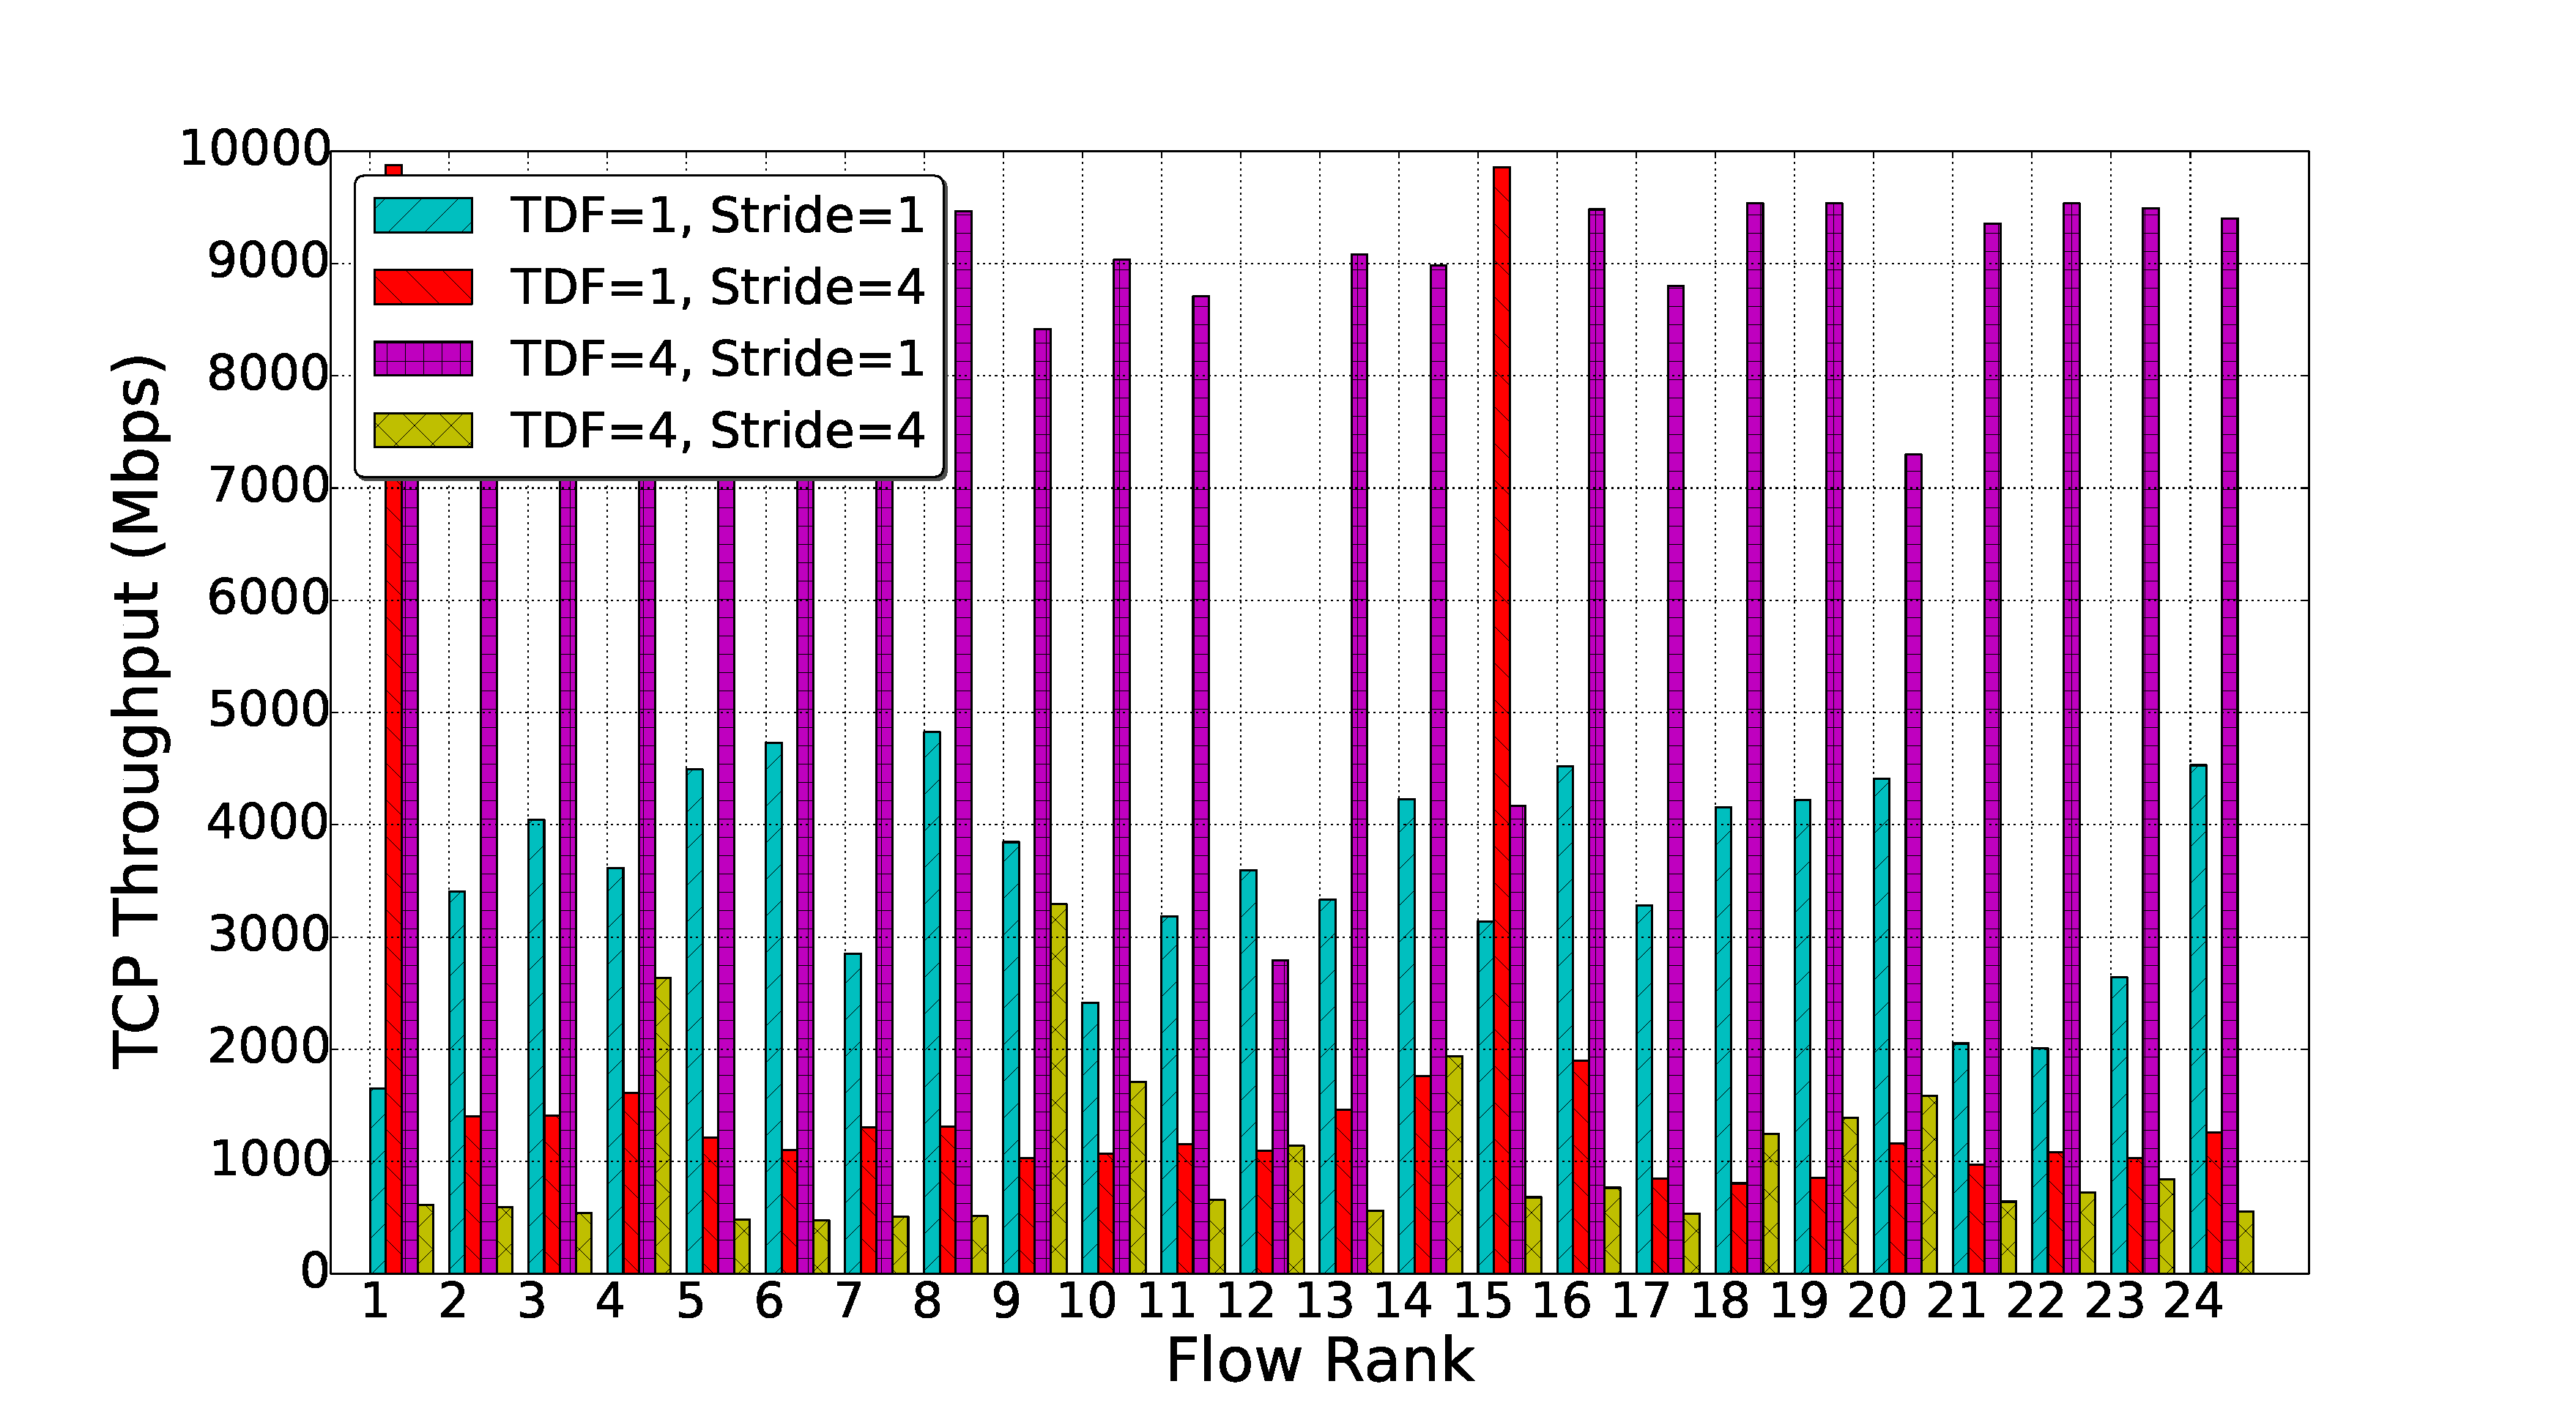
\epsfig{file=VirtualTime/figures/FattreeFlowDistBw10G.eps, width=0.45\textwidth}
    \label{VT:Fig:FatTreeIndividualBw10G}}
    \caption[Emulate ECMP with High Link Bandwdith]{Mininet Emulation Results with Virtual Time: ECMP Limitation in a Fat-tree-based Data Center Network with 10 Gbps Link Bandwidth}
\end{figure}

In the case of stride-1, there were very few collisions among flows.
Hence, the network performance ought to be close to the ideal throughput, i.e., 160 Gbps biSsection bandwidth and 10 Gbps average bandwidth between each pair.
In the experiments that $TDF=4$, the average throughput is above 9.0 Gbps, which is close to the theoretical value,
and also match well with the results obtained from the physical testbed built upon 37 machines~\cite{Hedera}.
In the experiments that $TDF=1$, however, the throughput barely reaches 3.8 Gbps because of the limited system resources that Mininet can utilize.
In addition, as shown in Figure~\ref{VT:Fig:FatTreeIndividualBw10G},
we observe that the variation of throughput is large among flows when $TDF=1$.
This is incorrect because no flow shares the same link in the case of stride-1.
In contrast, when $TDF = 4$, the throughput of all 8 flows are close with little variation, which implies the desired networking behaviors. 

In the case of stride-4, flows may collide both on the upstream and the downstream paths, thus using ECMP could undergo a significant throughput drop,
e.g., up to 61\% as experimentally evaluated in~\cite{Hedera}.
The virtual-time-enabled Mininet ($TDF=4$) has successfully captured such throughput drop phenomenon.
We can see that average throughput dropped about 80\% when RipL-Pox controller used ECMP to handle multi-path flows.
Large deviation (more than 55\% of average throughput value) also indicates that the flows were not properly scheduled with ECMP.
When $TDF=1$ (no virtual time), Mininet also reported plummeted TCP throughput in the case of stride-4.
However, we cannot use the result to experimentally demonstrate the limitation of ECMP.
It is hard to distinguish whether the throughput drop was caused by insufficient resources to handle 10 Gbps or the limitation of ECMP,
given the fact that the throughput was already too low in the collision-free case.
Without a correct baseline (benchmark for the collision-free scenario), it is difficult to perform further analysis and qualify the limitation.



\Section{Summary of Virtual Time System}
\label{VT:Sec:Conclusion}

In conclusion, we present a Linux-container-based virtual time system and integrated it to a widely used SDN emulator, Mininet.
The lightweight system uses a time-dilation-based design to offer virtual time to the containers,
as well as the applications running inside the containers with no code modification.
Experimental results show the promising fidelity and scalability improvement of Mininet with virtual time,
particularly for high workload network scenarios. We have also used the platform to precisely
evaluate the limitations of the ECMP routing in a realistic data center network with the results being validated by a physical testbed.
Our virtual time system has been adopted and extended by other emulation testbeds.
Minichain~\cite{Minichain}, a blockchain emulator designed to allow users to conduct
high-fidelity emulation experiments of a blockchain system concerning both application behaviors
and network characteristics at low cost, e.g., evaluating a new application design on a single laptop.
The main and unique challenge Minichain must address is how to execute
the heavy-duty proof-of-work based consensus algorithm with limited emulation resources.
It turns out one can put proof-of-work based blockchain emulation into virtual time where time dilation factor is less than 1.
As a result, emulation resources consumed by proof-of-work will decrease linearly as converged difficulty is scaled down linear.
Another extension to our virtual time system is to make it possible to put
multiple Linux embedded devices into virtual time and coordinates them~\cite{DistributedVT}.
This is motivated by the synchronization need of general cyber-physical system,
where physical components are simulated and cyber components are emulated.
Future works include the investigation of other effective control algorithms to further improve the adaptive TDF scheduler,
and the integration to network simulators based on virtual time for large-scale network analysis.


\clearpage

\Chapter{One Big Switch}
\label{Cpt:OBS}
\section{Motivation}

% Bring in the issues that our approach can address
% Describe them as problems in current simulation/emulation systems
Software defined networking (SDN) centralizes and simplifies control of network management,
and has been increasingly adopted in data centers and internet exchange points~\cite{B4, Meridian, SDX}.
%Software defined networking (SDN) technology separate the network control logic of the network from
%the distributed hardware that implementing the forwarding behaviors.
Similar to traditional computer network systems, it is crucial to perform appropriate testing and evaluation of
SDN-based applications before deploying on a real system.

Researchers in the simulation community have extended various existing network simulators to support SDN capability~\cite{S3F, NS3, OPNET}.
To improve experimental fidelity, researchers have also developed network emulation testbeds
(e.g., Mininet~\cite{Mininet}) that utilize Linux containers over shared hardware resources and
real network stack to run high-fidelity SDN experiments.
However, container-based emulators cannot reproduce the correct behavior of a real network
with a large network topology and high traffic load because of the limited underlying physical resources.
For example, on a commodity machine with 2.98 GHz CPU, 4 GB RAM, and 3 Gbps internal bandwidth,
Mininet can only emulate a network up to 30 hosts, each with a 100 MHz CPU, 100 MB RAM and connected by 100 Mbps links~\cite{ReproNetExprCBE}.
Therefore, increasing SDN testbed scalability and speed without losing the desired fidelity is essential.

% State our idea
In this paper, we present a model abstraction technique to transform an SDN-based network model to a ``one-big-switch'' network model.
This technique is useful if users only care about the end-to-end behavior rather than
the details within the network, such as hop-by-hop routing, or table lookup on each single switch.
For example, users may want to simulate a large-scale complex network of networks consisting of traditional TCP/IP networks,
SDN networks, industry control communication networks, etc.
The SDN components in this scenario may not be the focus, and thus maintaining only the end-to-end behavior is sufficient for running the hybrid experiment.
Our technique is also useful for real-time network simulation, in which models must be executed
no slower than the wall-clock time in order to interact with real implementations of network protocols and applications.
Failing to do so may result in temporal faults, i.e., the simulation fails to process events before the designated deadlines
required by the emulation or physical components. 
In addition, industrial collaborators may not want to disclose the details of their production network
(e.g., topology, routing, middle-box location and functionality) to modelers for privacy and security concerns.
They can use our model abstraction techniques on the target network and share the resulting ``one-big-switch'' model.

We develop a three-step approach to transform an SDN network to a big OpenFlow switch based network,
while still preserving the network forwarding logic equivalence.
The high-level idea is illustrated in Figure~\ref{OBS:Fig:BigSimOverview},
and the details are discussed in Section~\ref{OBS:Sec:Design}.
Our approach reduces the SDN network to a big-switch-based network to improve the scalability of SDN simulation or emulation.

\begin{figure}[t]
    \centering
    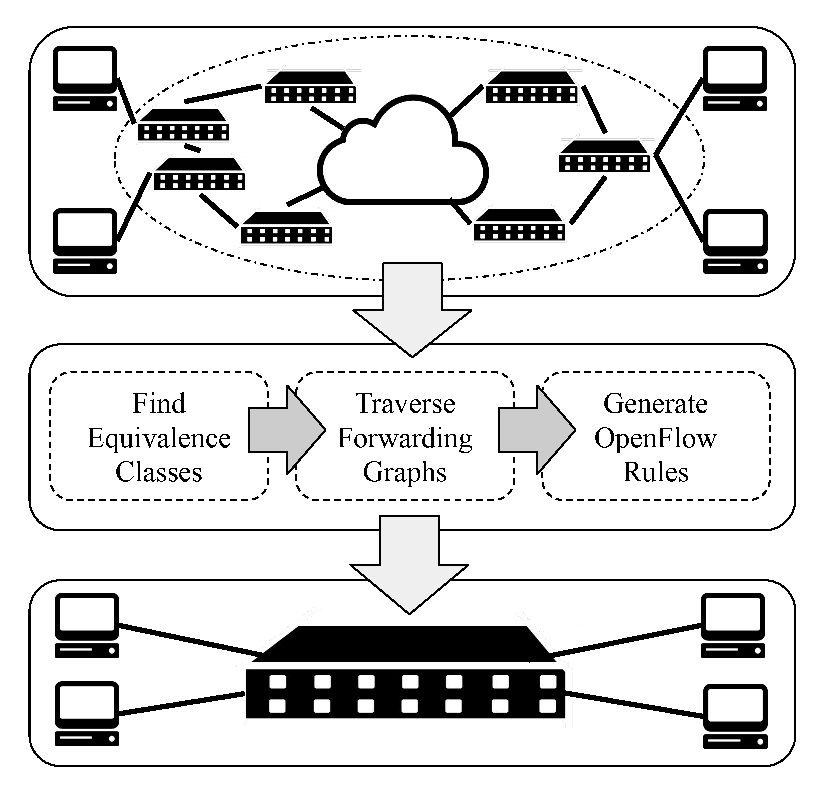
\includegraphics[width=0.9\textwidth]{OneBigSwitch/figures/BigSimOverview.eps}
    \caption[One Big Switch Abstraction Overview]{Transforming an SDN network to a
    big OpenFlow switch based network while preserving the network forwarding logic equivalence.}
    \label{OBS:Fig:BigSimOverview}
\end{figure}

The reduction in the number of switches and the number of rules significantly enhances the testbed scalability and reduces the experiment running time.
For example, after abstracting a tree-topology network of depth 4 and fanout 3,
the total number of switches required to simulate is reduced from 40 to 1, and the number of rules existed in the SDN network is reduced by 89\%.
The big-switch based network model can save about
75\% to 85\% simulation execution time as compared to simulating the original network.
We can also reuse the abstracted network model.
For example, after one complete experimental run of a complex network,
users can abstract (possibly part of) the network, and reproduce the simulation results with
a much simpler configuration, including link connectivity and flow tables.
We can partition a large-scale network model, and abstract each partition in parallel.
By combining those abstracted network models, a testing platform with limited hardware resources
now can afford such network simulation/emulation experiments.
As the network state evolves, the abstracted big-switch model may also need to be frequently updated.
Our approach is lightweight. For example, we can reduce 50,000+ rules in a large tree-topology network
to 5,000+ rules in a big-switch-based network in three seconds, 
while still preserving the network forwarding rule equivalence.
In addition, our approach allows incrementally updating the big-switch model,
i.e., modifying the rules that are only affected by the current network changes.

This chapter is organized as follows.
Section~\ref{OBS:Sec:MotivatingExample} illustrates the problem and the approach using a simple motivating example.
Section~\ref{OBS:Sec:Design} describes the details of the three-step model abstraction design.
Section~\ref{OBS:Sec:Evaluation} presents the evaluation results in terms of forwarding logic equivalence, simulation time,
reduction in flow rules, and model abstraction execution time.
Section~\ref{OBS:Sec:Conclusion} concludes this chapter.

\section{Motivating Example}
\label{OBS:Sec:MotivatingExample}

\tikzset {
    roundnode/.style={circle, draw=blue!80, fill=blue!5, very thick, minimum size=7mm},
        squarenode/.style={rectangle, draw=red!80, fill=red!5, very thick, minimum size=7mm},
        ->-/.style={->, line width=1.2pt},
        ==/.style={line width=1.6pt}
    }

\begin{figure}[t]
    \centering
    \begin{tikzpicture}
        \node[roundnode] (sw0) {SW0};
        \node[roundnode] (sw1) [below left=2cm of sw0] {SW1};
        \node[roundnode] (sw2) [below=1.1cm of sw0] {SW2};
        \node[roundnode] (sw3) [below right=2cm of sw0] {SW3};
        \node[squarenode] (net1) [below=1cm of sw1] {10.1.0.10/16};
        \node[squarenode] (net2) [below=1cm of sw2] {10.0.0.10/8};
        \node[squarenode] (net3) [below=1cm of sw3] {11.1.0.10/16};

        \draw[-, line width=1.2pt] (sw0) -- node [near start, above] {0} node[near end, below] {1} (sw1);
        \draw[-, line width=1.2pt] (sw0) -- node [near start, right] {1} node[near end, left] {1} (sw2);
        \draw[-, line width=1.2pt] (sw0) -- node [near start, above] {2} node[near end, below] {1} (sw3);
        \draw[-, line width=1.2pt] (sw1) -- node [near start, left] {0} (net1);
        \draw[-, line width=1.2pt] (sw2) -- node [near start, left] {0} (net2);
        \draw[-, line width=1.2pt] (sw3) -- node [near start, right] {0} (net3);
    \end{tikzpicture}
    \caption{A Tree-Topology SDN Network}
    \label{OBS:Fig:ExampleNetworkTopo}
\end{figure}

\begin{figure*}
    \centering
    \subfigure[Forwarding Graph for EC1 and EC3] {
        \begin{tikzpicture}
            \node[roundnode] (sw2) {SW2};
            \node[roundnode] (sw0) [left=of sw2] {SW0};
            \node[roundnode] (sw1) [above left=of sw0] {SW1};
            \node[roundnode] (sw3) [below left=of sw0] {SW3};
            \node[squarenode, align=center] (ec13) [right=of sw2] {EC1: 10.0.*.*\\EC3: 10.2.0.0-10.255.255.255};

            \draw[->-] (sw0) -- node [near start, above] {1} node[near end, above] {1} (sw2);
            \draw[->-] (sw1) -- node [near start, above] {1} node[near end, above] {0} (sw0);
            \draw[->-] (sw3) -- node [near start, above] {1} node[near end, above] {2} (sw0);
            \draw[->-] (sw2) -- node [near start, above] {0} (ec13);
        \end{tikzpicture}
    \label{OBS:Fig:ExampleForwardingEC13}
}

    \subfigure[Forwarding Graph for EC2] {
        \begin{tikzpicture}
            \node[roundnode] (sw1) {SW1};
            \node[roundnode] (sw0) [left=of sw2] {SW0};
            \node[roundnode] (sw2) [above left=of sw0] {SW2};
            \node[roundnode] (sw3) [below left=of sw0] {SW3};
            \node[squarenode] (ec2) [right=of sw1] {EC2: 10.1.*.*};

            \draw[->-] (sw0) -- node [near start, above] {0} node[near end, above] {1} (sw1);
            \draw[->-] (sw2) -- node [near start, above] {1} node[near end, above] {1} (sw0);
            \draw[->-] (sw3) -- node [near start, above] {1} node[near end, above] {2} (sw0);
            \draw[->-] (sw1) -- node [near start, above] {0} (ec2);
        \end{tikzpicture}
    \label{OBS:Fig:ExampleForwardingEC2}
}
    \subfigure[Forwarding Graph for EC4] {
        \begin{tikzpicture}
            \node[roundnode] (sw3) {SW3};
            \node[roundnode] (sw0) [left=of sw3] {SW0};
            \node[roundnode] (sw1) [above left=of sw0] {SW1};
            \node[roundnode] (sw2) [below left=of sw0] {SW2};
            \node[squarenode] (ec4) [right=of sw3] {EC4: 11.1.*.*};

            \draw[->-] (sw0) -- node [near start, above] {2} node[near end, above] {2} (sw3);
            \draw[->-] (sw1) -- node [near start, above] {1} node[near end, above] {0} (sw0);
            \draw[->-] (sw2) -- node [near start, above] {1} node[near end, above] {1} (sw0);
            \draw[->-] (sw3) -- node [near start, above] {0} (ec4);
        \end{tikzpicture}
    \label{OBS:Fig:ExampleForwardingEC4}
}
    \caption{Forward Graph for Each EC}
    \label{OBS:Fig:ExampleForwardingGraphs}
\end{figure*}

\begin{table*}[t]
    \caption{Forwarding Rules in the 3-ary Tree Network}
    \begin{center}
        \begin{tabular}{c|clc}
            \hline
            Switch & Priority & Match Field & Action\\
            \hline
            \hline
            \multirow{3}{2em}{SW0} & 10 & NW\_DST=10.1.*.* & FWD: OUT\_PORT=0 \\
                       & 1  & NW\_DST=10.*.*.* & FWD: OUT\_PORT=1 \\
                       & 1  & NW\_DST=11.1.*.* & FWD: OUT\_PORT=2 \\
            \hline
            \multirow{3}{2em}{SW1} & 10 & IN\_PORT=1, NW\_DST=10.1.*.* & FWD: OUT\_PORT=0 \\
                       & 1  & IN\_PORT=0, NW\_DST=10.*.*.* & FWD: OUT\_PORT=1 \\
                       & 1  & IN\_PORT=0, NW\_DST=11.1.*.* & FWD: OUT\_PORT=1 \\
            \hline
            \multirow{3}{2em}{SW2} & 10 & IN\_PORT=0, NW\_DST=10.1.*.* & FWD: OUT\_PORT=1 \\
                       & 1  & IN\_PORT=1, NW\_DST=10.*.*.* & FWD: OUT\_PORT=0 \\
                       & 1  & IN\_PORT=0, NW\_DST=11.1.*.* & FWD: OUT\_PORT=1 \\
            \hline
            \multirow{3}{2em}{SW3} & 10 & IN\_PORT=1, NW\_DST=11.1.*.* & FWD: OUT\_PORT=0 \\
                       & 1  & IN\_PORT=0, NW\_DST=10.*.*.* & FWD: OUT\_PORT=1 \\
                       & 1  & IN\_PORT=0, NW\_DST=10.1.*.* & FWD: OUT\_PORT=1 \\
            \hline
        \end{tabular}
    \end{center}
    \label{OBS:Tab:OriginalFlowTable}
\end{table*}

\begin{table*}[t]
    \caption{Forwarding Rules on the ``Big OpenFlow Switch"}
    \begin{center}
        \begin{tabular}{c|clc}
            \hline
            Switch & Priority & Match Field & Action\\
            \hline
            \hline
            \multirow{4}{2em}{SW}  & 10 & NW\_DST=10.0.*.* & FWD OUT\_PORT=1 \\
                       & 10 & NW\_DST=10.1.*.* & FWD OUT\_PORT=0 \\
                       & 10 & NW\_DST=11.1.*.* & FWD OUT\_PORT=2 \\
                       & 10 & NW\_DST=10.2.0.0-10.255.255.255 & FWD OUT\_PORT=1 \\
            \hline
        \end{tabular}
    \end{center}
    \label{OBS:Tab:CompressedFlowTable}
\end{table*}

In this section, we describe our model abstraction technique to transform an SDN network model to a big-switch model with a concrete network example.
Let us consider a tree-topology network connected by four OpenFlow switches, as shown in Figure~\ref{OBS:Fig:ExampleNetworkTopo}.
The centralized SDN controller (not shown in the figure for simplicity) installs the forwarding rules on each switch to establish connections for all three subnets.
All the switch rules are shown in Table~\ref{OBS:Tab:OriginalFlowTable}.
We assume that during the process of model abstraction, the rules have been installed on each OpenFlow switch,
and there is no link down or rule modification. OpenFlow switch 0 (i.e., SW0) works as an \textbf{aggregation switch}
that provides connectivity for other switches. SW1, SW2 and SW3 work as \textbf{edge switches} that provide connectivity for each subnet,
and each edge switch connects to one end-host.

Our approach abstracts the network to one big switch that has logically equivalent forwarding behavior.

The first step in the abstraction process is to extract \textit{equivalence classes} through the OpenFlow rules installed on network devices, i.e., aggregation and edge switches.
%As formally defined later in Section~\ref{Sec:Design} and in \cite{Veriflow},
Equivalence class (EC) is the set of packets that experience identical forwarding action at \textbf{all} network devices.
%This concept is proposed to confine network verification activities to the minimal effected set of packets\cite{Veriflow}.
We utilize EC to merge all the rules on a set of switches. For example, the flow rules shown in Table~\ref{OBS:Tab:OriginalFlowTable} can be sliced into
four \textbf{disjoint} ECs based on the NW\_DST field as follows. Note that the matching field IN\_PORT cannot be used in identifying ECs,
since it is not a packet-dependent, but topology-dependent field.

\begin{itemize}
    \item Packets in EC1 are destined to the network address 10.0.*.*.
    \item Packets in EC2 are destined to hosts with address 10.1.*.*.
    \item Packets in EC3 are destined to the address range from 10.2.0.0 to 10.255.255.255
    \item Packets in EC4 are destined to the subnet 11.1.*.*.
\end{itemize}

After identifying all the ECs from the rule set, we generate \textit{forwarding graph} for each EC, which models how packets within an EC are forwarded through the network~\cite{Veriflow}.
The node in a forwarding graph represents a network device, and the directed edge represents how the network device forwards the packets.
The sink nodes, i.e., the red rectangle nodes in Figure~\ref{OBS:Fig:ExampleForwardingGraphs}, indentifies the EC that this forwarding graph belongs to.
Each equivalence class will have exactly one forwarding graph, as shown in Figure~\ref{OBS:Fig:ExampleForwardingGraphs}.
%If we skip the process of minimizing number of ECs from the rules,
Note that \{EC1, EC2, EC3, EC4\} is not yet the minimal set of ECs in the network.
In fact, EC1 and EC3 can be merged because the forwarding behaviors of both ECs are identical at any device in the network,
as depicted in Figure~\ref{OBS:Fig:ExampleForwardingEC13} that EC1 and EC3 share the same forwarding graph.

We finish the model abstraction by generating a new set of forwarding rules that are to be installed on the big switch.
To make the process more efficient, we only have to consider those ECs whose packets traverse edge switches in the network.

Table~\ref{OBS:Tab:CompressedFlowTable} shows the resulting rules that will be installed in the big switch (see Figure~\ref{OBS:Fig:ExampleBigSwitch}).
The resulting one-big-switch network has the identical forwarding functions to the original tree network from the end-to-end communication perspective.
% in the eyes of the three hosts(possibly emulated or simulated).
The number of switches we need to simulate or emulate is now reduced from four to one, and the number of rules in the network is reduced from twelve to four.
If we only consider OpenFlow rules that match the NW\_DST field and the action is always forwarding,
then the total number of rules in the big switch is proportional to the number of ECs,
whereas in the original SDN network, the total number of rules is $O(S\times P)$,
where $S$ is the number of switches and $P$ is the number of address prefixes.

\begin{figure}[t]
    \centering
    \begin{tikzpicture}
        \node[roundnode, minimum size=15mm, align=center] (sw) {Big\\Switch};
        \node[squarenode, align=center] (ec13) [below=1.3cm of sw] {10.0.0.10/8};
        \node[squarenode] (ec2) [below left=2cm of sw] {10.1.0.10/16};
        \node[squarenode] (ec4) [below right=2cm of sw] {11.1.0.10/16};

        \draw[-, line width=1.2pt] (sw) -- node [near start, above] {0} (ec2);
        \draw[-, line width=1.2pt] (sw) -- node [near start, right] {1} (ec13);
        \draw[-, line width=1.2pt] (sw) -- node [near start, above] {2} (ec4);
    \end{tikzpicture}
    \caption{Compressed SDN Network for Scalable Simulation}
    \label{OBS:Fig:ExampleBigSwitch}
\end{figure}

\section{SDN Model Abstraction}
\label{OBS:Sec:Design}

\begin{comment}
    The overview of our model abstraction approach for SDN networks is shown in Figure~\ref{OBS:Fig:BigSimOverview}.
    Through a three-step systematic process, we are able to take
    a snapshot of an SDN network $SN$ as the input, transform the network devices in an SDN network to a single OpenFlow switch,
    $BS$ that preserves the forwarding logic of the original network.
    In this section, we elaborate the algorithmic design in each step of the model abstraction.
    %We have sketched the process of how to replace a OpenFlow-switch-connected network with a single OpenFlow switch in section~\ref{Sec:MotivationalExample}.
\end{comment}

Our objective is to effectively transform a static SDN data plane configuration (i.e., a snapshot of the network state)
to ``one-big-switch'' model, which preserves the same end-to-end forwarding behavior.
%In other words, if a packet originated from a host is forwarded to host in the snapshot, then the packet will be sent to the same destination by the ``big switch".
To achieve this objective, we need to identify how every packet is processed in the snapshot,
and how to correctly configure the big-switch model to reflect the identical forwarding logic.
In this paper, we develop a three-step model abstraction method, which is summarized as follows.

\begin{itemize}
    \item \textbf{Identifying Equivalence Classes.} We partition all possible packets in the network into mutually exclusive sets
        (i.e., equivalence class, as formally defined in Section~\ref{OBS:Sec:IdentifyEC}), and the packets belongs to the same set are processed in the same way.
        Those sets are identified according to the matching field of \textbf{all} the OpenFlow rules on \textbf{all} the SDN switches in the original network.
    \item \textbf{Creating Forwarding Graphs.} We model the forwarding behavior of each packet set using the topology information
        as well as the local information stored on SDN switches (e.g., port mapping, rule priorities, etc),
        and generate a graph-based model to represent the forwarding behavior.
    \item \textbf{Generating OpenFlow Rules of the Big Switch.} We generate the OpenFlow rules for the big switch
        in order to preserve the end-to-end forwarding logic.
        This step includes (1) constructing the port-to-host mapping,
        (2) generating the rules by matching the packet header of each set,
        and (3) forwarding the packet to the correct output port, which is determined by traversing the forwarding graph acquired in step 2.
\end{itemize}

Our three-step approach has two assumptions. First, the controller can dynamically change the configuration of each network device,
but we assume that the frequency of issuing such control messages is far less than the rate of the incoming packets.
Between two configuration updates, the data plane remains unchanged.
Therefore, we can exclude the SDN controller from the abstracted network model.
Second, we do not consider packet header modification actions on the network device.
We describe each step in details in the remainder of the section.

%We assume that both the original network and abstracted network use OpenFlow switches, and the switches compare the incoming packet to the installed rule with highest priority and then apply the action of that rule. The simplicity of OpenFlow switches enables us to analyze the behavior of the original network and synthesis the configuration of the ``big switch".

\subsection{Identifying Equivalence Classes}
\label{OBS:Sec:IdentifyEC}

By aggregating and slicing forwarding rules in an SDN network according to ECs, one can obtain a compact representation of the network state in terms of forwarding behavior.
We first give the definition of equivalence class (EC), and then present the data structure and algorithms to partition the packets into ECs.
\begin{definition}
    An equivalence class is a set of packets that experience identical forwarding action at \textbf{any} network device in the network.
    \label{OBS:Def:EC}
\end{definition}

\begin{comment}
    %\kevin{add to one or two sentences about how to find ECs and how to aggregate ECs before the structure}
    By its definition, ECs can be found by aggregate forwarding rules on different switches
    and group them by the match field.
    We aggregate forwarding rules using a trie structure as inspired by VeriFlow~\cite{Veriflow}.
    A trie node has three child nodes, i.e., zero, one or wildcard, that represent three possible values for performing a bit-to-bit rule matching.
    The entire tree is composited by several sub-tries, each representing one packet header field.
    For example, consider the tree-topology network in Section~\ref{OBS:Sec:MotivatingExample},
    the trie only contains one sub-trie representing the $NW\_DST$ header field (i.e., the network destination address).
    Note that an EC can be defined by multiple fields. For example, we can also match the source address of the packet (e.g., $NW\_SRC$)
    as well as the service type of the traffic ($TCP\_SRC$). The resulting trie now has three sub-tries.
    %Here we give solutions to two problems that VeriFlow neglected.
\end{comment}

Each packet is uniquely identified by its header field values, which are matched against the forwarding rules in the OpenFlow switches
to determine the appropriate action.
Since the matching fields of the OpenFlow rules typically contain the wildcard suffix (e.g., longest prefix match of IP source/destination addresses), a group of packets with consecutive header values are often processed by the same rule.
We use a trie structure, originally proposed by VeriFlow~\cite{Veriflow}, to maintain the matching fields of all the OpenFlow rules in the network.
The trie is composed of several sub-tries, and each sub-trie stands for a matching field (e.g., source/destination MAC address/IP address/port, etc.).
Each node in sub-trie presents one bit in the corresponding matching field, and each node has three edges to the next node (i.e., next bit in the  matching field).
The edges represent three possible bit-to-bit rule matching conditions: zero, one, or wildcard (i.e., don't care).
The rule metadata are stored in the corresponding leaf node, including the rule's location (i.e., switch index),
action (e.g., forwarding to an out port or dropping the packet), priority, etc.

Having all the OpenFlow rules inserted in the aforementioned trie structure,
we perform the following three steps to identify the equivalence classes in the network.
(1) We traverse the trie to obtain the consecutive header values for each rule.
(2) After having a collection of header value intervals, which are denoted by the starting and end values,
we develop an algorithm to split the existing intervals into smaller and non-overlapping intervals.
Each non-overlapping interval identifies the packets belonging to an equivalence class.
(3) We merge certain equivalence classes in order to reduce the time and space complexity for the forwarding graph generation
(Section~\ref{OBS:Sec:GenerateFG}) and the big-switch rule generation (Section~\ref{OBS:Sec:PopulateFlowTable}).
The details of the second and third steps for EC identification are presented as follows.

\paragraphbe{Splitting Overlapping Intervals}
By traversing from the root node to all leaf nodes, we obtain a set of packet header intervals that match all the rules along the traversal.
Each interval is represented by a pair of starting and ending values as $A, B$ and $C$ as shown in Figure~\ref{OBS:Fig:DisjointECsAsInterval}.
We split this set of intervals, $I$, to a list of non-overlapping intervals, each of which forms an EC.
%An example is shown in the upper part of Figure~\ref{Fig:DisjointECsAsInterval}.
We develop Algorithm~\ref{OBS:Alg:GenDisjointECs} to generate a set of disjoint intervals, and show that the generation can be
accomplished in $O(N \times M\log M)$ time,
where $M$ is the number of intervals in $I$, and $N$ is the number of header bits.
% as follows\cite{SplitDisjointInterval}.
%Not algorithmic described in\cite{Veriflow},

First, we place $I$ into an array $A$ of $2M$ elements. Each element is either a beginning value or an ending value of an interval. We denote the set of beginning values as $S$ and the set of ending values as $E$. We visit each value $x$ in a sorted order, and maintain the difference $d$ between the number of visited starting points and the number of visited end points.
\begin{itemize}
    \item If the current element $x \in S$ and $d > 0$,
        we finish processing the previous interval with the ending value $x - 1$ and
        create the next interval with a starting value $x$
        (line~\ref{OBS:Alg:LineEndStart1}-\ref{OBS:Alg:LineEndStart2}).
    \item If the current element $x \in E$, we end the previous interval with the ending value $x$.
        (line~\ref{OBS:Alg:LineEndEnd}).
    \item In either case, we update the potential new interval's starting value \textit{prev}
        (line~\ref{OBS:Alg:LineNewPrev1} and~\ref{OBS:Alg:LineNewPrev2}).
\end{itemize}
%\kevin{Please define $S$ and $E$, and ``end an interval" or "start an interval" does not sound right to me, usually we start/end an action.}

Updating the network forwarding rules will change the EC set.
By maintaining the rules in a trie, we can efficiently update ECs in an incremental way. An insertion of a new rule requires us to do a depth first traversal. This process automatically narrows down the set of affected rules by ignoring those non-overlapping branches with the new rule.
The output is the set of affected intervals, and we can run Algorithm~\ref{OBS:Alg:GenDisjointECs} to update only those affected ECs.

\begin{figure}[t]
    \centering
    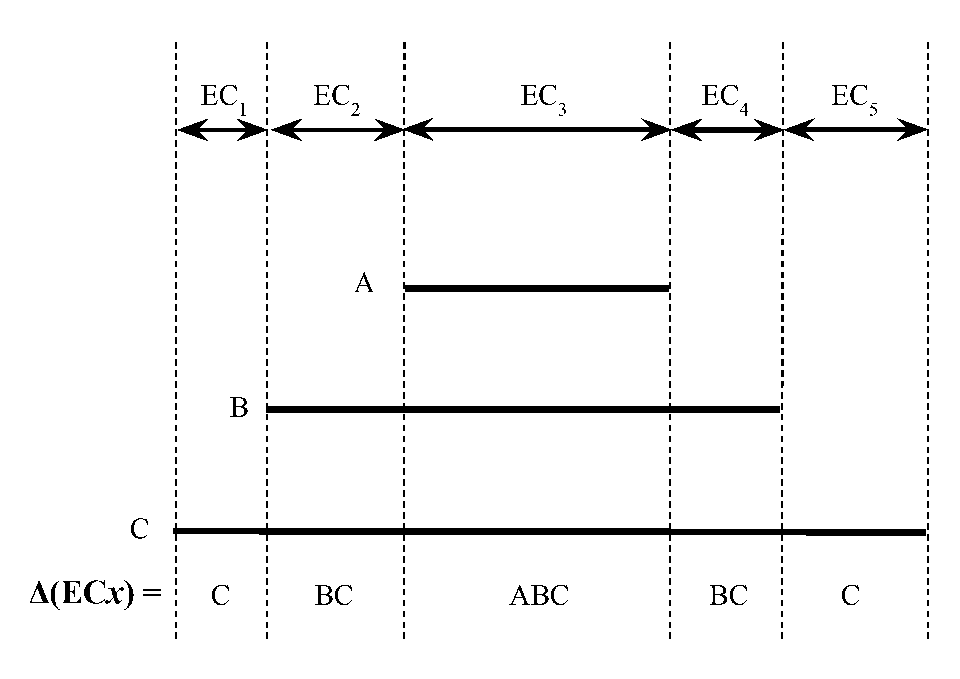
\includegraphics[scale=.52]{OneBigSwitch/figures/DisjointECs.eps}
    \caption[Equivalence Classes as Disjoint Intervals]{A set of packets are identified by
    an interval of packet header values.
    Five equivalence classes, $EC_1$ to $EC_5$, can be obtained via splitting three intervals
    A, B and C.
    Finding $\Delta[EC_x]$ (i.e., the rules that intersect with $EC_x$) is instrumental for
    merging ECs, as shown in the bottom of the figure.}
    \label{OBS:Fig:DisjointECsAsInterval}
\end{figure}

\begin{algorithm}[t]
    \DontPrintSemicolon
    \KwData{$I = $ a set of packet header intervals from the leaves of the trie}
    \KwResult{$D = $ a set of disjoint intervals as equivalence classes} 
    $cnt \gets 0$\;
    $S = $ \{beginning values of $\forall i \in I\}$\;
    $E = $ \{ending values of $\forall i \in I\}$\;
    $A \gets Sort(S \bigcup E)$ in a non-decreasing order\;
    $D \gets \emptyset$\;
    \ForEach {$x \in A$} {
        \uIf {$x \in S$} {
            \If {$cnt \neq 0$} {\label{OBS:Alg:LineEndStart1}
            $D \gets D \text{ }\bigcup \text{} [prev, x-1]$\;
            }\label{OBS:Alg:LineEndStart2}
            $prev \gets x$\;\label{OBS:Alg:LineNewPrev1}
            $cnt \gets cnt + 1$\;
        }
        \Else {
            $D \gets D \text{ } \bigcup \text{ } [prev, x]$\;\label{OBS:Alg:LineEndEnd}
            $prev \gets x + 1$\;\label{OBS:Alg:LineNewPrev2}
            $cnt \gets cnt - 1$\;
        }
    }
    \caption{Splitting Overlapping Intervals}
    \label{OBS:Alg:GenDisjointECs}
\end{algorithm}

\begin{algorithm}[h]
    \DontPrintSemicolon
    \KwIn{$nodes = $ Switches containing rules for EC $x$ \newline
    $topo = $ Network topology}
    \KwResult{Forwarding graph $FG(x)$ for EC $x$}
    \SetKwProg{Fn}{Function}{}{\KwRet}
    \SetKwFunction{Traverse}{traverse}
    \SetKwFunction{GenRule}{generate\_rules}
    \Fn{\Traverse{$curr$, $src$, $snk$}} {
        \uIf {$curr$ \upshape is \textbf{NOT} visited} {
            $r \gets$ \textbf{highest-priority} rule on $curr$ that processes EC $x$\;
            \If {r \upshape is NULL or $r.action$ is DROP} {\label{OBS:Alg:LineDropPath1}
            $snk \gets$ ($curr$, NULL)\;
            \GenRule{$x, src, snk$}\;
            \KwRet\;
            }\label{OBS:Alg:LineDropPath2}
            $next \gets topo[curr][r.action.outport]$\;
            \If {next $\not\in$ nodes} {\label{OBS:Alg:LineForwardPath1}
            $snk \gets$ ($curr$, $r.action.outport$)\;
            \GenRule{$x, curr, src, snk$}\;
            \KwRet\;
            }\label{OBS:Alg:LineForwardPath2}
            mark $curr$ as visited\;
            \Traverse{$next, src, snk$}\;
        }
        \Else {
            report forwarding loop\;\label{OBS:Alg:LineLoopPath}
        }
    }\;
    \ForEach{$n \in$ \upshape neighbors of $SRC^x$} {\label{OBS:Alg:LineStartDFS1}
    \If {\upshape $n$ is \textbf{NOT} visited} {
        $inport \gets$ input port number from $SRC^x$ to $n$\;
        \Traverse{$n$, $src=$\upshape($n$, $inport$), $snk=$NULL}\;
    }
    }\label{OBS:Alg:LineStartDFS2}
    \caption{Generating a Forwarding Graph for EC $x$\label{OBS:Alg:GenForwardingGraph}}
\end{algorithm}

\begin{algorithm}[h]
    \DontPrintSemicolon
    \KwData{$PortMap$, which maps a $port$ on $sw$ to a $port$ on the big switch\newline
    $global\_port$, for port number assignment, and is initialized to 0}
    \KwResult{A new rule $r$ to install on the big switch}
    \SetKwProg{Fn}{Function}{}{\KwRet}
    \SetKwFunction{GenRule}{generate\_rules}
    \Fn{\GenRule{$x, src, dst$}} {
        $r.match \gets x$\;\label{OBS:Alg:LineMatch}
        \If {src.port $\not\in$ PortMap[src.sw]} {
            $PortMap[src.sw][src.port] \gets global\_port++$\;
        }
        $r.inport = PortMap[src.sw][src.port]$\;\label{OBS:Alg:LineInport}
        \uIf {dst.port \upshape is NULL} {
            $r.action \gets $ drop\_action\;\label{OBS:Alg:LineGenDropRule}
        }
        \Else {
            \If {dst.port $\not\in$ PortMap[dst.sw]} {\label{OBS:Alg:LineGenForwardRule1}
            $PortMap[dst.sw][dst.port] \gets global\_port++$\;
            }
            $r.action \gets $ forward\_action\;
            $r.action.outport \gets PortMap[dst.sw][dst.port]$\;\label{OBS:Alg:LineGenForwardRule2}

        }
    }
    \caption{Generating Forwarding Rules for EC $x$ on the Big-Switch Model \label{OBS:Alg:GenAllRules}}
\end{algorithm}

\paragraphbe{Combining Equivalence Classes}
We can further union certain ECs obtained from Algorithm~\ref{OBS:Alg:GenDisjointECs},
if they essentially represent identical packet forwarding behavior (see the definition of ECs).
For example, $EC_2$ and $EC_4$ in Figure~\ref{OBS:Fig:DisjointECsAsInterval} can be combined as one EC,
since the packets in both ECs experience the same set of forwarding rules in the network.
%To generate the correct set of rules on the new ``big switch", we only need to model the forwarding behavior of either one of the ECs. In other words, for any two ECs $\alpha$ and $\beta$, we have:

\begin{lemma}
    If packets in EC $\alpha$ and EC $\beta$ experience the same forwarding actions on all network devices, then $\alpha \cup \beta$ is also an EC.
    \label{OBS:Lemma:MergeFG}
\end{lemma}
Combining two EC into a single one reduces the running time in the next two phases, i.e., generating the forwarding graph and populating the final OpenFlow rules. The number of the resulting forwarding rules in the big switch can also be reduced. We present the following lemma to identify whether two ECs can be unioned.

\begin{lemma}
    EC $\alpha$ and EC $\beta$ can be unioned into one EC, if both packet header values are covered by the same set of rules in the network.
    \label{OBS:Lemma:MergeEC}
\end{lemma}
%According to Lemma~\ref{Lemma:MergeEC},
For example, both $EC_2$ and $EC_4$ are covered by interval $B$ and $C$ in Figure~\ref{OBS:Fig:DisjointECsAsInterval}, and therefore, we can treat them as one EC. The explanation is illustrated below.

First, we define a function $\Delta(x)$ that maps an EC $x$ to a set of forwarding rules, whose matching fields cover the header values of all the packets in $x$. Assume $\Delta(\alpha) = \Delta(\beta)$, and let $\delta \in \Delta(\alpha)$ be the rule on a network device $d$ with the highest priority.
If no such $\delta$ exists, packets from both $\alpha$ and $\beta$ are dropped on $d$.
Otherwise, packets in both $\alpha$ and $\beta$ match the rule $\delta$ and are processed with the same action specified in $\delta$.
Note that in another device $d'$, the highest priority rule that covers both $\alpha$
and $\beta$ may be different, i.e., $\delta' \neq \delta$.
However, as long as $\delta$ is unique at a given $d$, the forwarding behavior at $d$ for both $\alpha$ and $\beta$ are always identical.

Given an EC, we can efficiently calculate $\Delta(\alpha)$ using two data structures: an array of pointers and a central interval tree.
Each of them is responsible for one of the two cases specified in~\cite{FindIntersectionWiki}.
\begin{itemize}
    \item Case 1: A rule $\delta$ overlaps with an EC $\alpha$ with its beginning and/or ending value in $\alpha$.
        We can reuse the sorted array $A$ in Algorithm~\ref{OBS:Alg:GenDisjointECs}.
        We augment each value, either a beginning value or an ending value of an interval in $A$ with a pointer to the corresponding rule.
        By doing a binary search, we can find the minimum and maximum values in $A$,
        which bound the interval of $\alpha$.
        %All intervals that overlap with $\alpha$ must be between the minima and maxima,
        Therefore, we can ignore two types of rules: the ones with ending values smaller than the minima and the ones with beginning values larger than the maxima.
        We then perform a linear search in the new set of rules, and check one-by-one whether the interval overlaps with $\alpha$.
        The total time complexity for both the linear search and the binary search are $O(\log M + K)$,
        where $K$ is the number of reported intervals in $\Delta(\alpha)$.

    \item Case 2: Rule $\delta$ covers $\alpha$ entirely. We can build
        a central interval tree~\cite{ComputationalGeometryBook} with all the available intervals.
        We pick a random value $x \in \alpha$ and query the central interval tree for
        all the ranges that intersect with $x$, which can be done in $O(\log M + K)$ time. It takes $O(M log M)$ time to build the central interval tree.
        Since the central interval tree supports efficient incremental operations (i.e., insertion and deletion), our design also supports dynamic changes of the rule set.
\end{itemize}

Using the interval tree and the ordered list, for each EC $\alpha$,
we calculate $\Delta(\alpha)$ by mapping each rule $\delta \in \Delta(\alpha)$ to a unique binary ID $c_\delta$ of length $\log_2 M$.
We can encode $\Delta(\alpha)$ to a string of $c_\delta$s, starting with small IDs.
This string of unique IDs, named $C_\alpha$, has a $M\log_2 M$ upper bound in length.
We then use a hash table $H$ to combined the ECs by hashing each EC $x$ to $C_x$.
The minimal size of ECs is the number of unique keys in $H$.
Note that in the subsequent algorithmic designs, iterating through all ECs refers to iterating through the first ECs in each set $H[key]$.%, $\forall key \in H$.

\subsection{Generating Forwarding Graphs}
\label{OBS:Sec:GenerateFG}

In the second step, we compute a forwarding graph for each EC, and then effectively reduce the size of the forwarding graph to improve efficiency for the third step.

First, we define a function $FG(\alpha)$ that maps an EC $\alpha$ to a corresponding forwarding graph. A forwarding graph is a directed graph that represents how packets belonging to the same EC are processed by the network. A node $u$ in the forwarding graph is a networking device, and an edge $(u, v)$ in the graph means that device $u$ forwards the packets to device $v$ in the network.
A forwarding graph not only concatenates the forwarding behavior for each EC, but also visualizes the data flow of the EC in the network.
%For a fixed EC $x$, we connect the network devices that have rules for $x$ with directed edges that point to the next hop, which is determined by the action field of the rule.
Since our objective is to abstract the network forwarding logic into a big switch, our end-to-end modeling focuses on the sources and sinks of the graph.
Figure~\ref{OBS:Fig:ForwardingGraphECX} depicts the generalized forwarding graph $FG(x)$ for EC $x$.

%Here we discuss two specific issues in the forwarding graph generation: where to start the traversal according to our needs and what we can achieve at the end of the traversal.

\begin{figure*}
    \centering
    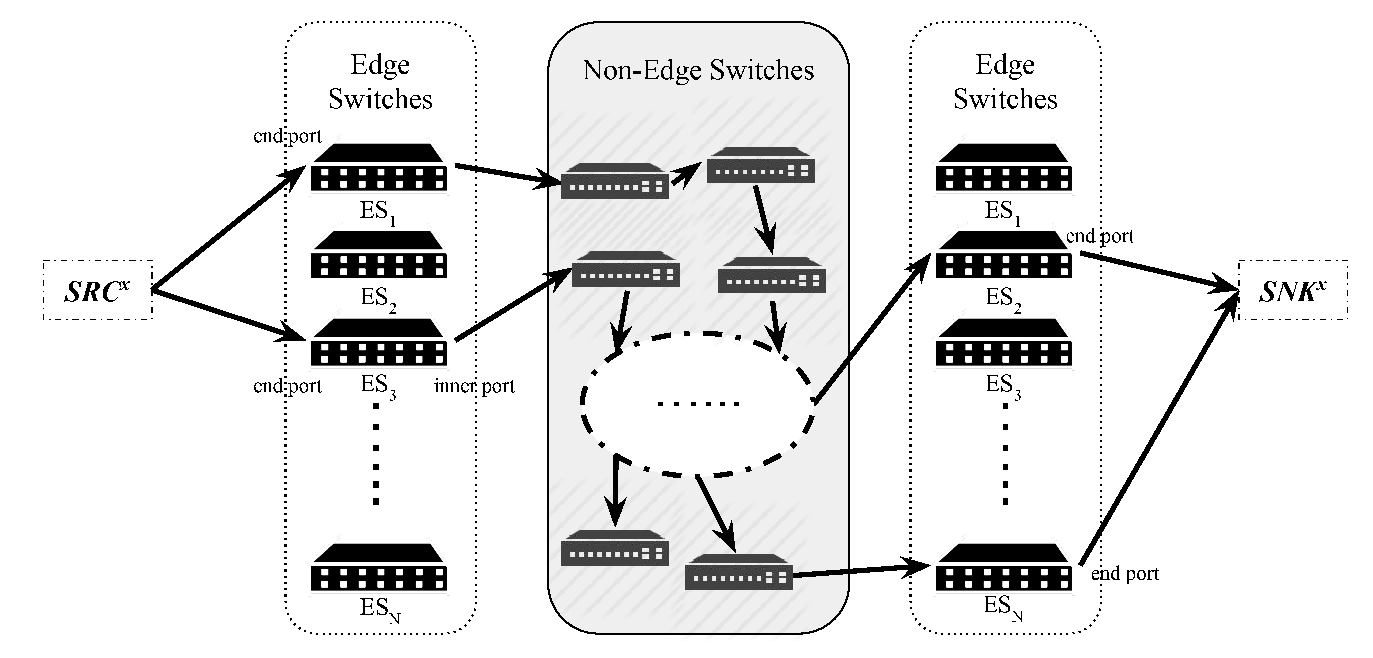
\includegraphics[width=0.9\textwidth]{OneBigSwitch/figures/ForwardingGraph.eps}
    \caption{Modeling a Forwarding Graph of an Equivalence Class}
    \label{OBS:Fig:ForwardingGraphECX}
\end{figure*}

\paragraphbe{Network Traversal for Forwarding Graph Generation.}
We develop a forwarding graph generation algorithm as shown in Algorithm~\ref{OBS:Alg:GenForwardingGraph}.
The notations are defined as follows.
$FG(x)$ denotes the forwarding graph for a particular equivalence class x.
A \textit{edge switch} is defined as a switch that has at least one link to a node located outside of the original network. 
%\kevin{$SN$ first appeared here, need definition.}
A \textit{non-edge switch} is defined as a switch with all connected nodes that are inside of the original network.
The forwarding behavior of the non-edge switches are not considered in the big-switch model abstraction.
Let $src$ and $snk$ denote the source and sink nodes of the forwarding path for an EC.
Note that all $src$ in $FG(x)$ are edge switches,
and $snk$ in $FG(x)$ can be either edge switches or non-edge switches.
Let $curr$ denote the current traversed node in the network.
We add a super-source node, $SRC^x$, and a super-sink node, $SNK^x$, as the boundaries of $FG(x)$.

Algorithm~\ref{OBS:Alg:GenForwardingGraph} is designed to generate $FG(x)$.
We start the process from each $src$ that connects to $SRC^x$,
and then traverse EC $x$'s forwarding graph using a depth-first-based search and
follow the action specified in the forwarding rule with the highest priority for EC $x$ at each node along the traversal.

%(2) the inner graph may contain both edge and internal switches.
%Source node $src$ and its out-going edge represent an edge switch $sw$ that forwards EC $x$ \textbf{coming from} port $p$; it can be described by $(sw, p)$ pair. Sink node $snk$ represent the end of the forwarding $sw$, which is also denoted by $(sw, p)$, where $p$ is either the port number specified by the action field or \texttt{NULL} if there is no rule for $x$ on $sw$.
%We denote the set of source nodes as $SRC(x)$, the set of sink nodes as $SNK(x)$.

We distinguish two kinds of port on an edge switch:
\begin{itemize}
    \item \textit{end port} that connects to a node that is either the forwarding end point or outside the target network;
    \item \textit{inner port} that connects to a node inside the target network.
\end{itemize}

We add an edge from $SRC^x$ to a $src$, if the source node has a forwarding rule $r$ that matches EC $x$, or the $IN\_PORT$ field of rule $r$ on the source node is an end port.
Otherwise, we do not initiate a traverse (see line~\ref{OBS:Alg:LineStartDFS1} to~\ref{OBS:Alg:LineStartDFS2} in Algorithm~\ref{OBS:Alg:GenForwardingGraph}).
Correspondingly, we add an edge from a $snk$ to the super sink $SNK^x$, if the following two conditions are satisfied:
\begin{enumerate}
    \item the sink node is an edge switch in the network;
    \item the $OUT\_PORT$ field determined by the rule's action on the sink node is an end port.
\end{enumerate}

\paragraphbe{Network Traversal Outcomes}
After running Algorithm~\ref{OBS:Alg:GenForwardingGraph}, we can discover three kinds of ``paths" in $FG(x)$
that are useful for the forwarding rule generation process for the big-switch model,
i.e., the third step of our model abstraction process (see Section~\ref{OBS:Sec:PopulateFlowTable}).

\begin{itemize}
    \item \textbf{Forwarding path} (line~\ref{OBS:Alg:LineForwardPath1}-\ref{OBS:Alg:LineForwardPath2}).
        The path from the super source node to the super sink node.
        This is a normal forwarding path for packets in EC $x$.

    \item \textbf{Dropping packets in the network} (line~\ref{OBS:Alg:LineDropPath1}-\ref{OBS:Alg:LineDropPath2}).
        The path ends at a device inside the network, and fails to reach the super sink node. This indicates that the packets in EC $x$ are dropped inside the network.

    \item \textbf{Forwarding loop} (line~\ref{OBS:Alg:LineLoopPath}).
        There is a directed cycle in the graph. One can simulate a forwarding loop in the network by (1) adding a rule in the big switch to drop the looping packets; or (2) dynamically monitoring the volume of the looping packets and adjusting the delay of looping packets and other packets sharing the communication path. We choose the first method since the model abstraction in the paper is focus on the forwarding logic equivalence, and will leave the second method as future work when investigating end-to-end performance equivalence.
        %This behavior can be emulated in the semantic of \textbf{performance equivalence}, but not by \textbf{logical equivalence} studied in this paper.
        %(1) recording the volume of the looping packets;
        %(2) increasing the delay of other packets on the basis of the amount of looping packets
\end{itemize}

\subsection{Populating Flow Tables on the Big-Switch Model}
\label{OBS:Sec:PopulateFlowTable}

We develop an algorithm to generate OpenFlow rules on the big switch to abstract the forwarding behavior (see Algorithm~\ref{OBS:Alg:GenAllRules}).
%by calling \texttt{generate\_rules}, as described in Algorithm~\ref{Alg:GenAllRules}.
We maintain a hash table $PortMap$ to map the end ports of the edge switches to the ports of the big switch.
This table is configured using the $global\_port$ variable during the rule generation procedure.
Algorithm~\ref{OBS:Alg:GenAllRules} generates the mandatory fields in an OpenFlow rule:
\begin{itemize}
    \item The $MATCH$ field is given by the EC $x$, i.e., the range of matching packets header (line~\ref{OBS:Alg:LineMatch});
    \item The $IN\_PORT$ field is the mapped port number of $src.port$ (line~\ref{OBS:Alg:LineInport});
    \item Depending on the $dst$ port, we generate either a packet drop action (line~\ref{OBS:Alg:LineGenDropRule}) or
        a packet forwarding action with the appropriate mapped port number of $dst.port$ (line~\ref{OBS:Alg:LineGenForwardRule1}-\ref{OBS:Alg:LineGenForwardRule2}).
\end{itemize}

\Section{Evaluation}
\label{OBS:Sec:Evaluation}

\begin{figure*}[ht]
    \centering
        \subfigure[$\mathcal{R}_1$, packets received per host in $net_1(d=2, f=3)$] {
            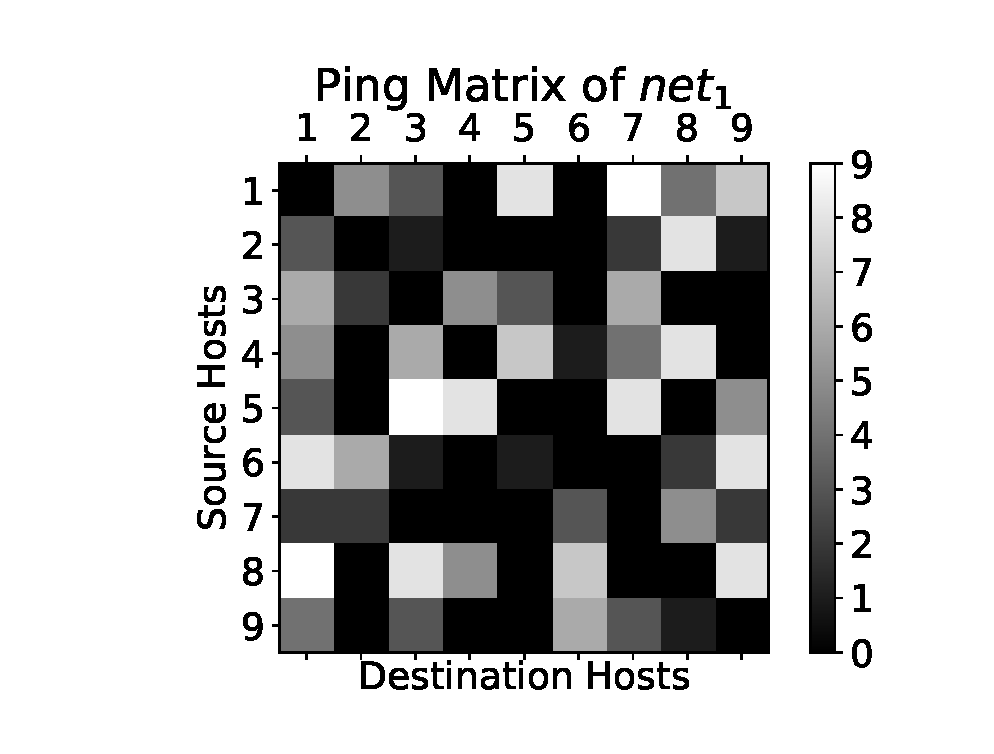
\includegraphics[width=.45\textwidth]{OneBigSwitch/figures/ping_mat_2_3.eps}
                \label{OBS:Fig:PingMatrix1}
            }
        \subfigure[$\mathcal{R}_2$, Packets received in $net_2(d=2, f=3)$] {
            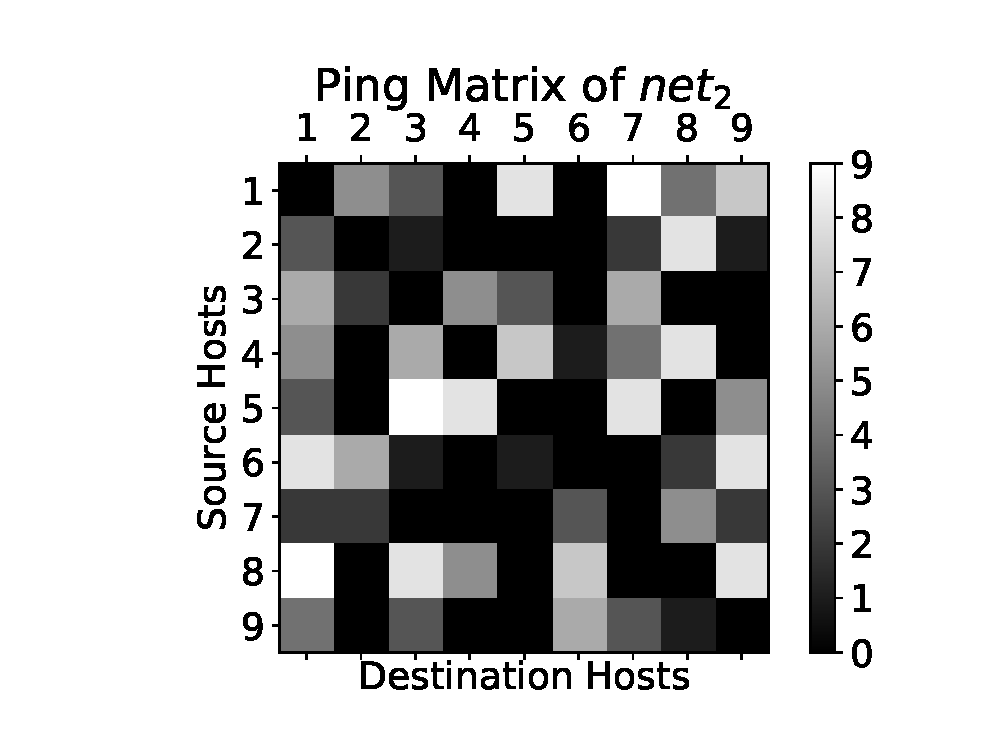
\includegraphics[width=.45\textwidth]{OneBigSwitch/figures/bs_ping_mat_2_3.eps}
                \label{OBS:Fig:PingMatrix2}
            }
        \\
        \subfigure[$\mathcal{R}_1$, Packets received in $net_1(d=4, f=3)$] {
            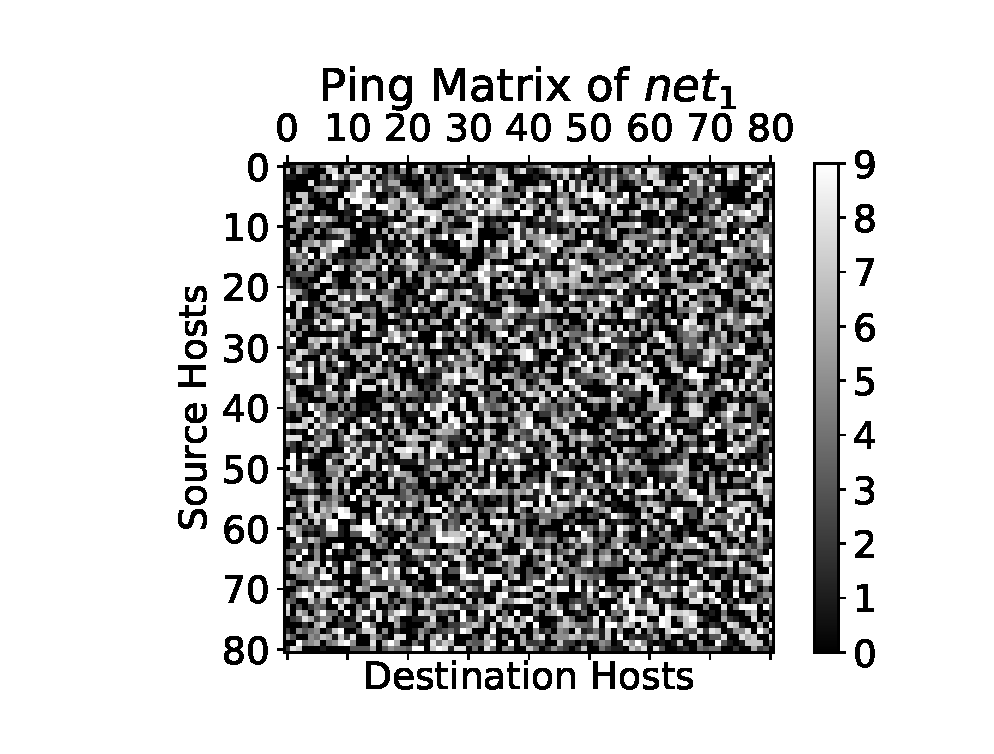
\includegraphics[width=.45\textwidth]{OneBigSwitch/figures/ping_mat_4_3.eps}
                \label{OBS:Fig:PingMatrix3}
            }
        \subfigure[$\mathcal{R}_2$, Packets received in $net_2(d=4, f=3)$] {
            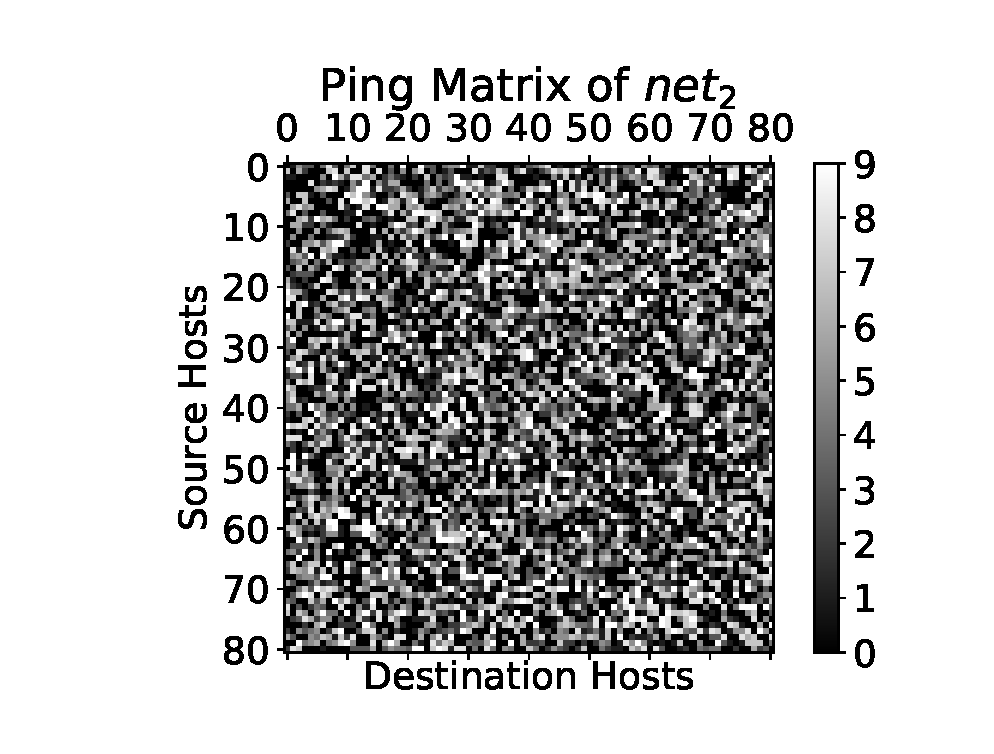
\includegraphics[width=.45\textwidth]{OneBigSwitch/figures/bs_ping_mat_4_3.eps}
                \label{OBS:Fig:PingMatrix4}
            }
        \caption[Forwarding Logic Evaluation after One-Big-Switch Abstraction]{
            Matrix $\mathcal{R}$ represents the number of packets received at each host.
        $net_1$ is the original SDN network with a tree topology ($d$, $f$),
        where $d$ is depth and $f$ is fanout.
        $net_2$ is the corresponding one-big-switch-based network.
        The gradient legend visualizes the number of received packets.
        $\mathcal{R}_1$ and $\mathcal{R}_2$ are identical,
        which indicate that our model abstraction technique preserves the network forwarding logic.}
    \label{OBS:Fig:ComparePingMatrix}
\end{figure*}

\begin{figure}[ht]
    \centering
    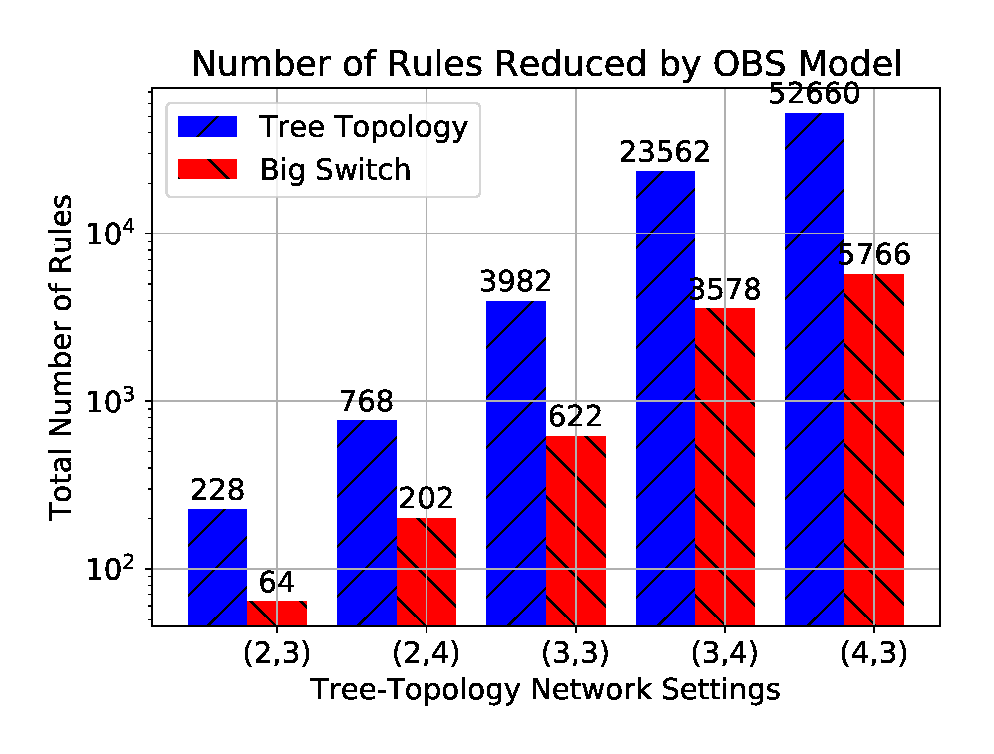
\includegraphics[width=0.9\textwidth]{OneBigSwitch/figures/comp_num_rules.eps}
    \caption[Number of Rules Reduced after One-Big-Switch Abstraction]{Number of rules needed to preserve the network forwarding logic.
        The number of rules on the big switch is about 72\% to 89\% less than
        the number of rules in the original tree-topology network.
        The x-axis label ($d$, $f$) represents the depth and fanout parameters
        in a tree topology network.}
    \label{OBS:Fig:CompareNumRules}
\end{figure}


\begin{figure}[ht]
    \centering
    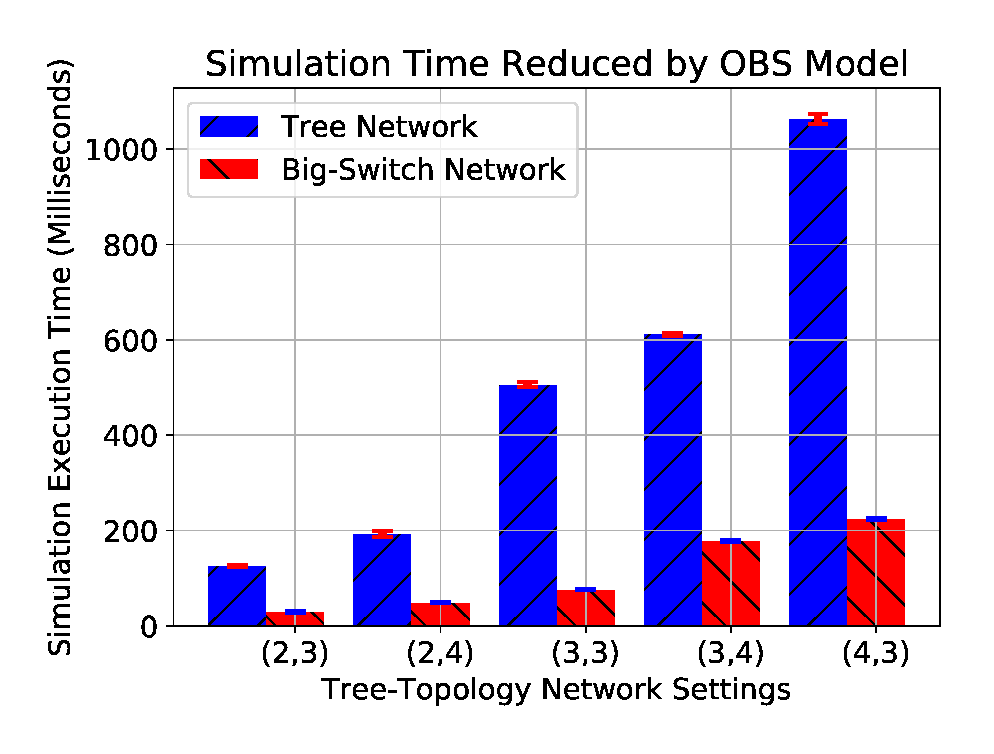
\includegraphics[width=0.9\textwidth]{OneBigSwitch/figures/comp_sim_time.eps}
    \caption[Comparison of Simulation Execution Time]{Comparison of simulation execution time.
        The big-switch-based network model saves about 75\% to 85\% running time
        as compared to simulating the corresponding SDN-based network.
        The x-axis label ($d$, $f$) represents the depth and fanout parameters in a tree topology network.}
    \label{OBS:Fig:CompareSimulationTime}
\end{figure}

\begin{figure}[ht]
    \centering
    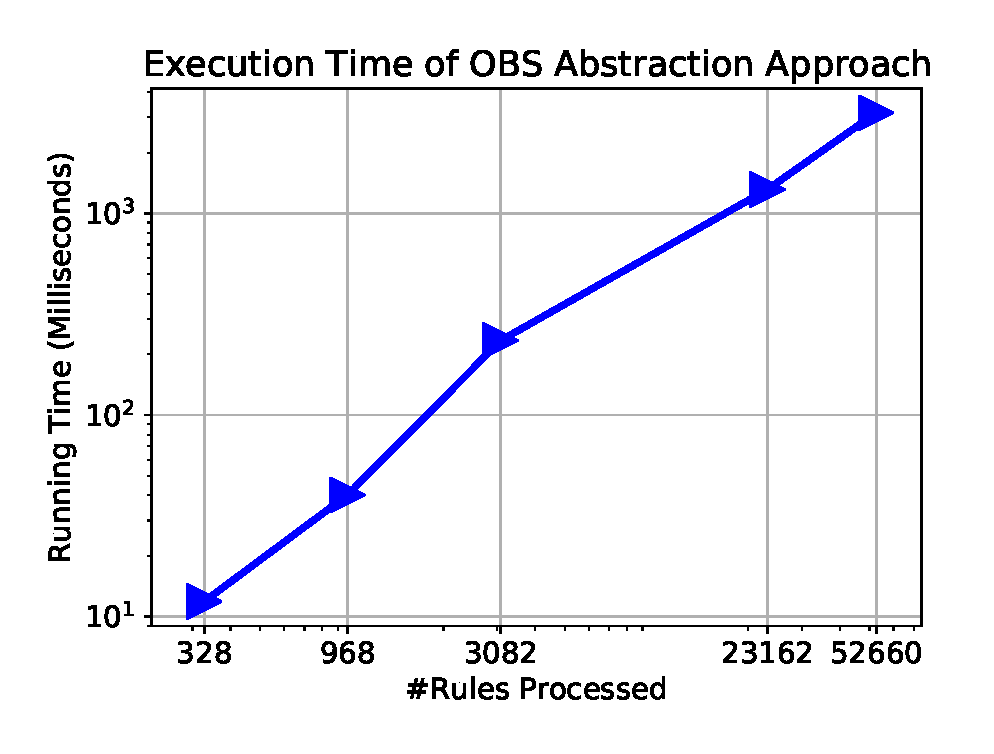
\includegraphics[width=0.9\textwidth]{OneBigSwitch/figures/bs_overhead.eps}
    \caption[Execution Time of One-Big-Switch Abstraction]{Execution time to transform an SDN-based network to a big-switch-based network.}
    \label{OBS:Fig:BSOverhead}
\end{figure}

\Subsection{Network Forwarding Logic Equivalence}
\label{OBS:SubSec:PreserveForwardingLogic}
We perform experimental evaluation of our network model abstraction technique
that transforms an SDN-based network to one-big-switch model.
The evaluation results show that our approach significantly saves simulation/emulation resources
(e.g., number of forwarding rules) and simulation execution time,
while still preserving the forwarding behavior of the original network.

Our experiments simulate and emulate networks of type tree topology.
The tree network is described by two topological parameters: depth $d$ and fanout $f$.
Such network $tree(d, f)$ can connect $f^d$ hosts with $\frac{f^d - 1}{f-1}$ switches in total.
%Though not known as a scalable network architecture (a good scalable alternative will be fat-tree topology), it is good for demonstration purpose since the tree topology is well-structured and
All end-hosts in a tree network are fully-connected with at most $2d$ hops.


We first demonstrate that the forwarding logic of the original software-defined network is exactly preserved by the abstracted big-switch model.
%One can find the shortest path between a pair of hosts $(s, d)$ with a layer-two learning switch controller application. Traversing the tree up and down in breadth-first-search style, learning switch application can automatically install OpenFlow rules on each hop once we initiate \texttt{ping} between the given pair of host. More specifically,
\if 0
\hl{
    Since the production SDN network snapshot, including topology connections and rules installed on
individual switches, are not easy to obtain, our demonstration is based on the following plausible setup.
}
\fi
We created a tree-topology network $net_1$ in Mininet~\cite{Mininet},
and connected all the switches to an SDN controller running a layer-two learning switch application~\cite{Pox}.
%We generated the network forwarding rules by establishing communication paths between random selected host pairs.
%For any network host $s$, we randomly generate a list of distinct hosts $dsts$, and let $s$ \texttt{ping} each host $dst \in dsts$.
After performing the \texttt{ping} tests between randomly selected pairs of end-hosts,
the controller application generated all the network forwarding rules and installed them on the switches.
We then took a snapshot of the network, including (1) the host-to-switch and switch-to-switch connections,
and (2) the rules on all the switches using the \texttt{ovs-ofctl dump-flows} command. The snapshot was used to generate the rules for the big-switch model as well as the port mapping according to the algorithms presented in Section~\ref{OBS:Sec:Design}.

We then created another emulated network $net_2$ in Mininet, consisting of one OpenFlow switch and the same number of hosts as $net_1$.
The switch was connected to $f^d$ hosts with the port numbers derived from both the $PortMap$ (Algorithm~\ref{OBS:Alg:GenAllRules})
and the link information ($net_1$'s topology).
The rules generated by Algorithm~\ref{OBS:Alg:GenAllRules} were installed on the switch using the \texttt{ovs-ofctl add-flow} command.

To validate that the big-switch-network preserved the network forwarding logic of the original network,
we recorded the connectivity between \emph{every} host pair in both $net_1$ and $net_2$,
and compared the results.
Specially, the original network $net_1$ is a tree network with $f^d$ hosts,
where $d$ is the depth and $f$ is the fanout of a tree network.
Each host sent a number of \texttt{ping} packets to every other host in $net_1$,
and the amount of packet was randomly selected between 1 and 10.
We repeated the experiments in $net_2$ with the same traffic pattern.
The result was represented in a matrix $\mathcal{R}$,
where $\mathcal{R}[i][j]$ denotes the numbers of successfully received \texttt{ping}
packets from host $i$ to host j, where $i \neq j$, and $i, j \in [1, f^d]$.

%To prevent l2\_learning switch controller from installing new rules in $net_1$, we take down the pox controller in this stage.
%The result of this experiment is a matrix $\mathcal{R}_k$ where $\mathcal{R}[i][j]$ denote

We repeated the experiment for different combinations of $d$ and $f$, i.e., ($d, f$) $\in$
\{(2, 3), (2, 4), (3, 3), (3, 4), (4, 3)\}. For each network scenario,
we saved the experimental results in $\mathcal{R}_1$ and $\mathcal{R}_2$, and compared the two matrices using the \texttt{diff} command.
We found that $\mathcal{R}_1 = \mathcal{R}_2$ holds true for all five network scenarios.
We visualized $\mathcal{R}_1$ and $\mathcal{R}_2$ for the ($d=2, f=3$) and ($d=4, f=3$) cases
in Figure~\ref{OBS:Fig:ComparePingMatrix}.
We can see that the original SDN-based network and the abstracted one-big-switch-based
network have the identical network forwarding logic,
measured by the connectivity and the number of receiving packets for each connection.
%In Figure~\ref{Fig:PingMatrix1}-Figure~\ref{Fig:PingMatrix4},
Note that the brightness of the element in the matrix is proportional to $\mathcal{R}[i][j]$,
i.e., the number of successfully delivered packets from host $i$ to host $j$.
%It is easy to see that $\mathcal{R}_1$ and $\mathcal{R}_2$ are identical for all experiment settings.

\Subsection{Performance Gain}
We show performance gain with two metrics.

\textbf{Number of OpenFlow Rules.} We compare the total number of rules installed
on the switches in both $net_1$ and $net_2$ with the same experimental settings
in Section~\ref{OBS:SubSec:PreserveForwardingLogic}.
The results are plotted in Figure~\ref{OBS:Fig:CompareNumRules} for networks with
various topological parameter settings.
%Note that y-axis is in log scale.
The number of rules needed to preserve the forwarding logic is significantly
less in the one-big-switch-based network as compared with the original SDN-based network
for all scenarios in the range of 71.93\% to 89.05\% reduction.
%approximately one degree of magnitude less than the number of rules existing in the original tree-topology network.
For example, in the case of a network with depth = 4, and fanout = 3, 52,660 rules
in the original network were reduced to 5,766 rules in the big-switch-based network.


\textbf{Simulation Time.}
Our approach significantly reduces network simulation model complexity in terms of
the number of switches and the number of rules.
A key benefit is to reduce the time to run simulation experiments.

We performed the same set of experiments on a network simulator, S3FNet~\cite{S3F}.
We simulated two SDN-based networks: one models a tree-topology network $net_1(d, f)$,
and the other models the corresponding big-switch-based network $net_2$.
We set half of the hosts as TCP clients and the other half as TCP servers,
and conducted one-to-one communication among them.
We sent each traffic flow for 100 seconds in simulation time.
We repeated each experiment ten times and recorded the simulation execution time for both $net_1$ and $net_2$ in
Figure~\ref{OBS:Fig:CompareSimulationTime} for comparison.
The error bars indicate the standard deviations of the running time
for all ten independent simulation runs.
We can see that simulating the big-switch-based network is 3.42 to 6.68 times
faster than simulating the original SDN-based network.


\Subsection{Model Abstraction Execution Time}
We discussed the asymptotic time complexity of our model abstraction technique in 
Section~\ref{OBS:Sec:Design}.
We now evaluate the execution time for transforming an SDN-based network to a big-switch-based network.
We recorded the running time for converting various tree networks,
i.e., ($d, f$) $\in$ \{(2, 3), (2, 4), (3, 3), (3, 4), (4, 3)\} in Figure~\ref{OBS:Fig:BSOverhead}.
We can see that the model abstraction process is lightweight.
For example, it took about 40 milliseconds to abstract a small tree network ($d=4$, $f=2$);
for a medium-scale medium-scale tree network (depth 4 and fanout 3),
it took about 3.15 seconds to process 52,660 rules.
The fast model abstraction execution time is useful.
As the network state keeps evolving, it is essential to constantly update the abstracted big-switch model to reflect the changes, preferably in an online fashion.
In fact, the three-step approach allows us to incrementally update the big-switch model and requires far less execution time, i.e.,
we only need to update a small set of rules that are different in the new network snapshot.


\Section{Summary of One-Big-Switch Abstraction}
\label{OBS:Sec:Conclusion}

We present a three-step model abstraction technique to transform an SDN-based network to
an ``one-big-switch'' based network without losing the forwarding behavior as
defined by the OpenFlow rules in the network devices.
Experimental results demonstrate that the big-switch abstraction correctly models
the end-to-end forwarding logic of the original SDN network,
and the abstracted model significantly saves the experiment running time and system resources.
The ultimate goal of the one-big-switch abstraction is to enhance simulation and emulation scalability while preserving packet-level fidelity.
This paper mainly focuses on the end-to-end for- warding logic equivalence,
and we will investigate end-to-end performance equivalence, such as latency and packet drop in the future.


\clearpage

\Chapter{Deep Learning for Network Intrusion Detection}
\label{Chp:DLNID}
\section{Deep Learning Background}

We introduce two main reasons behind the success of deep learning to the rise of artificial intelligence
as well as the implications of deep learning for network intrusion detection.

In the supervised learning framework, given the feature representations and inference models,
learning is an optimization process that minimizes a predefined loss function over the training examples.
The most commonly-used optimization algorithm is back-propagation (BP)~\cite{Backpropagation} with gradient descent,
because computing gradient is Hessian-free and memorization saves a significant amount of computation when propagating backward level by level.
However, it is challenging to train deep neural networks with optimal weights only using BP.
The first problem is that the cost function is usually non-convex, and
optimizing algorithms only with the first-order gradient is likely to be stuck at a poor local minimum.
Secondly, exploding and vanishing gradient makes back-propagation difficult to train models with many layers stacked together,
such as deep recurrent neural networks.
Even if we can tolerate the long training time and carefully deal with the gradient exploding and vanishing,
the trained model is often over-fitted to the training dataset, and thus fails to generalize to the testing or future datasets.

The emergence of many novel learning algorithms and training techniques enables us to train deep neural networks that achieve good suboptimal minimums.
For example, stochastic gradient descent (SGD) with mini-batches can significantly increase the training speed comparing
to normal gradient descent on the entire dataset.
In each step of gradient descent, researchers have shown that momentum can
prevent SGD from ``oscillating across but pushing along the shallow ravine"~\cite{Momentum}.
Along with decaying learning rate, momentum-based optimization algorithms (e.g., Adam~\cite{Adam}) often find better local minimums.
To prevent over-fitting, researchers have proposed dropout~\cite{Dropout} to average over an exponential number of neural networks.
These general learning algorithms and training techniques would directly help neural networks to achieve better performance for the network intrusion detection problem.

Another breakthrough in the deep learning area is that researchers have successfully trained a number of useful unsupervised generative models.
Different from supervised models or discriminative models that aim to discover the relationship between
input variables and target labels (or the conditional probability distribution of the targets given the inputs),
these models aim to learn the joint probability distribution or the joint conditional distribution of all variables for one phenomenon from the given dataset.
The resulting generative model is powerful in many ways.
First, given the well-trained probability distribution, the model can synthesize meaningful data comparable to real examples in the training set.
For example, Auxiliary-Classifier Generative Adversarial Nets (AC-GAN)~\cite{AC-GAN} can generate high-quality images after training on ImageNet dataset~\cite{ImageNet};
both AC-GAN and deep brief nets~\cite{DeepBeliefNets} can synthesize handwritten digits after learning from the MNIST dataset.
Second, the ability to generate high quality faked data indicates that
the model has learned better feature representations from the unlabeled data.
For example, the features extracted from the hidden units of sparse autoencoder can significantly improve the performance of support vector classifier~\cite{SparseAE}.
Additionally, researchers have shown that it is an excellent strategy to initialize deep neural networks
with the weights from a successfully trained generative model~\cite{DeepBeliefNets, Momentum}.

In the area of network intrusion detection, the amount of network traffic data is massive,
%e.g., in the order of terabytes per day in a large monitored network. In practice, the amount of data is 
which makes it hard for security analysts to find malicious patterns and label anomalies.
This situation makes the unsupervised generative model a promising solution
to traffic classification. %since it can be trained unsupervised:
First, it utilizes the vast amount of unlabeled data to learning useful and hierarchical features. Second, it effectively initializes the weights of the hidden layers in a deep neural network, which allows further fine-tuning towards a high-performance classifier.
Among the various deep learning models we investigate in this paper, there are two types of generative models, i.e., restricted Boltzmann machine and autoencoders.

%In addition to the sophisticated and efficient learning algorithms, abundant open data in the domain of image classification, natural language processing, or machine translation actually drive the novel and complex neural network models and make them successful.
%Table~\ref{Tab:Datasets} lists the dimension and amount of the training dataset for various image classification tasks.

\iffalse
The most vivid example would be how ImageNet dataset~\cite{ImageNet} pushed a series of deep learning models,
such as AlexNet, GoolgNet and ResNet, who greatly improved the performance of visual object recognition.
ImageNet organizes a large amount of web images by synonym set, multiple words or word phrases
describing a meaningful concept.
On average each synonym set is illustrated by 1000 quality-controlled and human-annotated images.
This project was first presented at 2009 Conference on Computer Vision and Pattern Recognition by researchers
from the CS department at Princeton University, and ran as an annual software contest known as
ImageNet Large Scale Visual Recognition Challenge (ILSVRC) since 2010.
The state-of-the-art error rate of this competition was near 25\%,
until in the year of 2012, a deep convolutional neural networks AlexNet~\cite{AlexNet} trained on GPU achieved a winning top-5 error rate of 15.3\%.
From then on, deep neural networks with convolutional blocks start its showtime.
GooLeNet~\cite{GoogLeNet} won the ILSVRC 2014 with top-5 error rate of 6.7\%.
It has 22 layers and strayed from the simple design of stacking convolutional and pooling layers.
One year later, residual block based ResNet~\cite{ResNet} pushed the error rate further down to 3.6\% with even deeper architecture.
\fi

%\begin{table*}[]
%\centering
%\caption{Popular Datasets used in Deep Learning v.s. Available Network Traffic Datasets}
%\label{Tab:Datasets}
%\begin{tabular}{c|c|c|c|c}
%\multicolumn{1}{c|}{Domain}                          & Dataset Name  & \#Examples in Training Set & Feature Dimension            & Instance-Feature Ratio \\
%\hline
%\hline
%\multirow{6}{*}{Image}                               & MNIST         & 60,000        & 784 (28$\times$28 gray images)            & 76.53    \\
%& SVHN          & 600,000       & 3072 (32$\times$32 color images)          & 195.31   \\
%& CIFAR-10      & 60,000        & 3072 (32$\times$32 color images)          & 19.53    \\
%& Tiny          & 80 million    & 3072 (32$\times$32 color image            & 26041.67 \\
%& ImageNet      & 1.2 million   & 196,608 (256$\times$256 color images)     & 18.31   \\
%\hline
%\multicolumn{1}{l|}{\multirow{2}{*}{Network Traffic}} & UNSW-NB15    & 175,341       & 42                                        & 4174.79 \\
%\multicolumn{1}{l|}{}                                 & NSL-KDD      & 125,973       & 41                                        & 3072.51
%\end{tabular}
%\end{table*}


\Section{Off-line Network Intrusion Detection Tasks}

Unlike image classification or natural language processing,
the labeled datasets in network intrusion detection tasks lacks a common feature space~\cite{KDDCup, DARPA, UNSW, NSL-KDD}.
For example, between the two datasets NSL-KDD\cite{NSL-KDD} and UNSW-NB15~\cite{UNSW},
we only identify five common features, i.e., src\_bytes, dst\_bytes, service, flag and duration.
As a result, we have to consider each dataset as a standalone network intrusion detection task.
We choose NSL-KDD and UNSW-NB15 datasets as our targeted tasks.
Table~\ref{CDL:Tab:Datasets} summarizes both tasks' training datasets along with some famous image classification datasets for comparison.

\Subsection{NSL-KDD Dataset}
The NSL-KDD dataset originates from the KDDCup 99 dataset~\cite{KDDCup},
but addresses two issues of the KDDCup 99 dataset.
First, it eliminates the redundant records in the KDDCup 99, i.e., 
78\% of the training set and 75\% of the testing set.
Second, it samples the dataset so that the number of records belonging to one difficulty level is inversely proportional to its difficulty.
The changes make the NSL-KDD dataset suitable for evaluating intrusion detection systems.
The training dataset consists of 125,973 TCP connection records, while the testing dataset consists of 22,544 records.
A record is defined by 41 features, including 9 basic features of individual TCP connections, 13 content features within a connection, 9 temporal features computed within a two-second time window, and 10 other features.
Connections in the training dataset are labeled as normal or one of the 24 attack types.
There are additional 14 types of attacks in the testing dataset, intentionally designed to test the classifier's ability to handle unknown attacks.
A classifier identifies whether a connection is normal or belongs to one of the four categories of attacks, namely denial-of-service (DoS), remote-to-local (R2L), user-to-root (U2R), and probing (also known as the 5-class classification problem).

\Subsection{UNSW-NB15 Dataset}
Similar to the KDDCup 99 dataset, the UNSW-NB15 dataset is generated by simulating normal and attack behaviors in a hardware testbed.
The simulation is conducted in the Cyber Range Lab of the Australian Centre for Cyber Security (ACCS) and
49 features in the dataset are extracted by a chain of software tools developed by ACCS.
The structure of the features is similar to that of KDDCup 99 including 5 flow features, 13 basic features, 8 content features, 9 time features, and 12 other features.
However, there are only five common features between to the UNSW-NB15 and NSL-KDD datasets.
The dataset has 257,673 flow records, among which 175,341 are used for
training set and the rest are for testing.
There are nine types of attacks in the dataset.
The only type of attack in common between UNSW-NB15 and NSL-KDD is DoS.
The new attacks in UNSW-NB15 are analysis, backdoor, exploits, fuzzers, generic, reconnaissance, shellcode, and worms.
In this paper, we consider the 2-class classification problem for the UNSW-NB15 dataset. The task is to predict whether a given flow record is normal or malicious.

\begin{table}[ht]
    \centering
    \caption[Network Intrusion Detection Datasets]{Image Datasets v.s. Network Intrusion Detection (NIDS) Datasets}
    \label{CDL:Tab:Datasets}
    \begin{tabular}{lcccc}
        \hline
        \hline
        \multicolumn{1}{l}{Domain}                          & Dataset       & Training Examples & Testing Examples & Feature Dimension  \\
        \hline
        \multirow{4}{*}{Image}                              & MNIST         & 60,000            & 10,000           & 784                \\
                                                            & SVHN          & 73,257            & 26,032           & 3072               \\
                                                            & CIFAR-10      & 50,000            & 10,000           & 3072               \\
                                                            & ImageNet      & $\approx$1.2 M    & $\approx$ 0.2 M  & 196,608            \\
        \cline{1-2}
        \multicolumn{1}{l}{\multirow{2}{*}{NIDS}}           & UNSW-NB15     & 175,341           & 82,332            & 42                \\
        \multicolumn{1}{l}{}                                & NSL-KDD       & 125,973           & 22,544            & 41                \\
        \hline
    \end{tabular}
\end{table}


\section{Deep Learning Models for Network Intrusion Detection}
\label{CDL:Sec:Architectures}

We explore a bunch of deep learning models that are promising to the
network intrusion detection problem, including multilayer perceptron, restricted boltzmann machine, sparse autoencoder, and wide and deep learning with embeddings. We develop a Python library, NetLearner~\cite{NetLearner}, which allows us to build and train those deep learning models using TensorFlow~\cite{TensorFlow}.

\subsection{Multilayer Perceptron}
\label{CDL:SubSec:MLP}
Multilayer perceptron (MLP) is a fully connected feed-forward neural network with multiple hidden layers.
Each layer consists of non-linear neural units.
By introducing non-linear neural units (perceptrons), it can distinguish data that are not linearly separable.
However, the non-linearity make it challenging to train a deep MLP of more than three layers even with the back-propagation learning algorithm~\cite{Backpropagation}.
MLP-based models get revived recently because of various training techniques designed by the deep learning community, including Stochastic Gradient Descent (SGD), Adam optimizer~\cite{Adam},
batch normalization~\cite{BatchNorm}, and Dropout~\cite{Dropout}.
Besides the number of neurons in each layer and the number of layers,
MPL can also be tuned with different activation functions or neural types.
In this paper, we use the logistic function and rectifier linear unit.

We build two dual-hidden-layer MLPs with 800 neurons in the first layer and 480 neurons in the second layer followed by a softmax classifier.
One MLP is for the NSL-KDD task, and the other is for the UNSW-NB15 task.
Both MLPs are trained with Adam optimizer~\cite{Adam} for 160 epochs with a batch size of 80.
During the training, the learning rate decays from 0.1 exponentially with the base of 0.96.
We do not include regularization in the model, but we apply dropout of probability 0.2 to prevent over-fitting.


\subsection{Restricted Boltzmann Machine}
Restricted Boltzmann machine (RBM)~\cite{DeepBeliefNets} is a type of energy-based models, which associate a scalar energy to each configuration vector of the variables in the network.
In an energy-based model, learning is the process of configuring the network weights to minimize the average energy over the training data.
Both Boltzmann machine and RBM consist of a layer of hidden units connected to a layer of visible units.
The term ``restricted" means that the connections are between the hidden and visible layers, but not within the hidden or visible layers.
Thus, RBM has faster training speed than Boltzmann machine, and it is feasible to stack multiple separately-trained RBMs to form a deeper neural network.
However, the classical way to train RBM is computational infeasible because it relies on a large number of iterations of alternating Gibbs sampling.
\cite{DeepBeliefNets} proposed contrastive divergence (CD-$x$) as a faster learning procedure.
They discover that instead of doing the alternating Gibbs sampling for many iterations,
applying $x$ (a small number between 1 and 4, say) steps of the alternating Gibbs sampling can quickly obtain a set of good weights for both layers.

For each task, we build an RBM with 800-hidden units to perform unsupervised learning on the training dataset.
We train the RBM using CD-1 with a batch size of 10 for 160 epochs.
The learning rate is initialized to 0.01 and it decays by 10e-6 over each gradient update.
We create a separate MLP with the same configuration described in Section~\ref{CDL:SubSec:MLP}, and initialize its weights in the first hidden layer (800 neurons equivalently) to those in the RBM model with the goal of improving the quality of MLP.
We then fine-tune the MLP for 160 epochs with a small learning rate of 0.01.


\iffalse
RBM consists of a layer of hidden units (H) and a layer of visible units (V).
Here ``restricted" means that connections are just between hidden and visible layer,
but not within hidden layers or visible layers.
This makes its training to be faster than Boltzmann machine and makes it feasible to
stack multiple separately trained RBM together to form deep architecture.
A joint configuration, $(\mathbf{v, h})$, of the visible and hidden units has the energy of
\begin{align}
    E(\mathbf{v, h}) &= -\sum_{i\in visible}a_i v_i - \sum_{j\in hidden}b_j h_j - \sum_{i, j}v_i h_j w_{ij}
\end{align}
where $a=\{a_i\}$ and $b=\{b_j\}$ are biases in visible and hidden layer respectively,
and $W=\{w_{ij}\}$ is the weights between them.
The network assigns a probability to every possible pair of $(\mathbf{v, h})$ via this energy
function
\begin{align}
    p(\mathbf{v, h}) &= \frac{1}{Z} e^{-E(\mathbf{v, h})} \\
    p(\mathbf{v}) &= \frac{1}{Z} \sum_{\mathbf{h}} e^{-E(\mathbf{v, h})}
\end{align}
where $Z$ is the partition function that equals to the summation over all possible hidden
and visible vector pairs
\begin{align}
    Z = \sum_{\mathbf{v,h}} e^{-E(\mathbf{v, h})}
\end{align}
Based on the ``maximizing log likelihood" idea,
we want to raise the probability of a training example and it can be done by
adjusting the weights biases to lower the energy of the considered example.
Meanwhile, we can let other examples make a big contribution to the partition function $Z$
by raising their energy.
Both insights can be translated to the following formula:
\begin{align}
    \frac{\partial \log p(v)}{\partial w_{ij}} = \langle v_i h_j \rangle_{data} - \langle v_i h_j \rangle_{model} 
\end{align}
This implies the following learning rule for performing stochastic gradient ascent on training
data
\begin{align}
    \Delta w_{ij} &= \varepsilon (\langle v_i h_j \rangle_{data} - \langle v_i h_j \rangle_{model})
\end{align}
The first term $\langle v_i h_j \rangle_{data}$ is the sampling from the data and it is easy to
compute since there is no directed connection between hidden units.
The sampling of $h_j$ is based on the probability
\begin{align}
    Prob(h_j = 1 | \mathbf{v}) &= sigmoid(b_j + \sum_i{v_i w_{ij}})
    \label{Equ:RBMSampleHidden}
\end{align}
Similarly, $v_i$ can be sampled with the following distribution
\begin{align}
    Prob(v_i = 1 | \mathbf{h}) &= sigmoid(a_j + \sum_j{h_i w_{ij}})
    \label{Equ:RBMSampleVisible}
\end{align}
The term $\langle v_i h_j \rangle_{model}$ can be obtained by performing alternative Gibbs
sampling for a long time.
The sampling starts from a random visible state.
Then we update the hidden units in parallel with Equation~\ref{Equ:RBMSampleHidden},
followed by updating the visible units in parallel with Equation~\ref{Equ:RBMSampleVisible}.
Instead of doing alternating Gibbs sampling for a large number of iterations,
\cite{TrainCD} proposed contrastive divergence (CD) as a faster learning procedure.
The training also start with a training vector to compute the states of the hidden units
using Equation~\ref{Equ:RBMSampleHidden}.
Then, with the chosen hidden states, we reconstruct the visible states by sampling each $v_i$
with probability given in Equation~\ref{Equ:RBMSampleVisible}.
The change of weight is then computed by
\begin{align}
    \Delta w_{ij} = \varepsilon (\langle v_i h_j \rangle_{data} -
    \langle v_i h_j \rangle_{reconstruct})
    \label{Equ:RBMCD1}
\end{align}
This is called contrastive divergence using one full step of alternating Gibbs sampling.
Contrastive divergence with $n$ rounds of alternating Gibbs sampling
is usually denoted as CD$n$.

\begin{figure}[h]
    \centering
    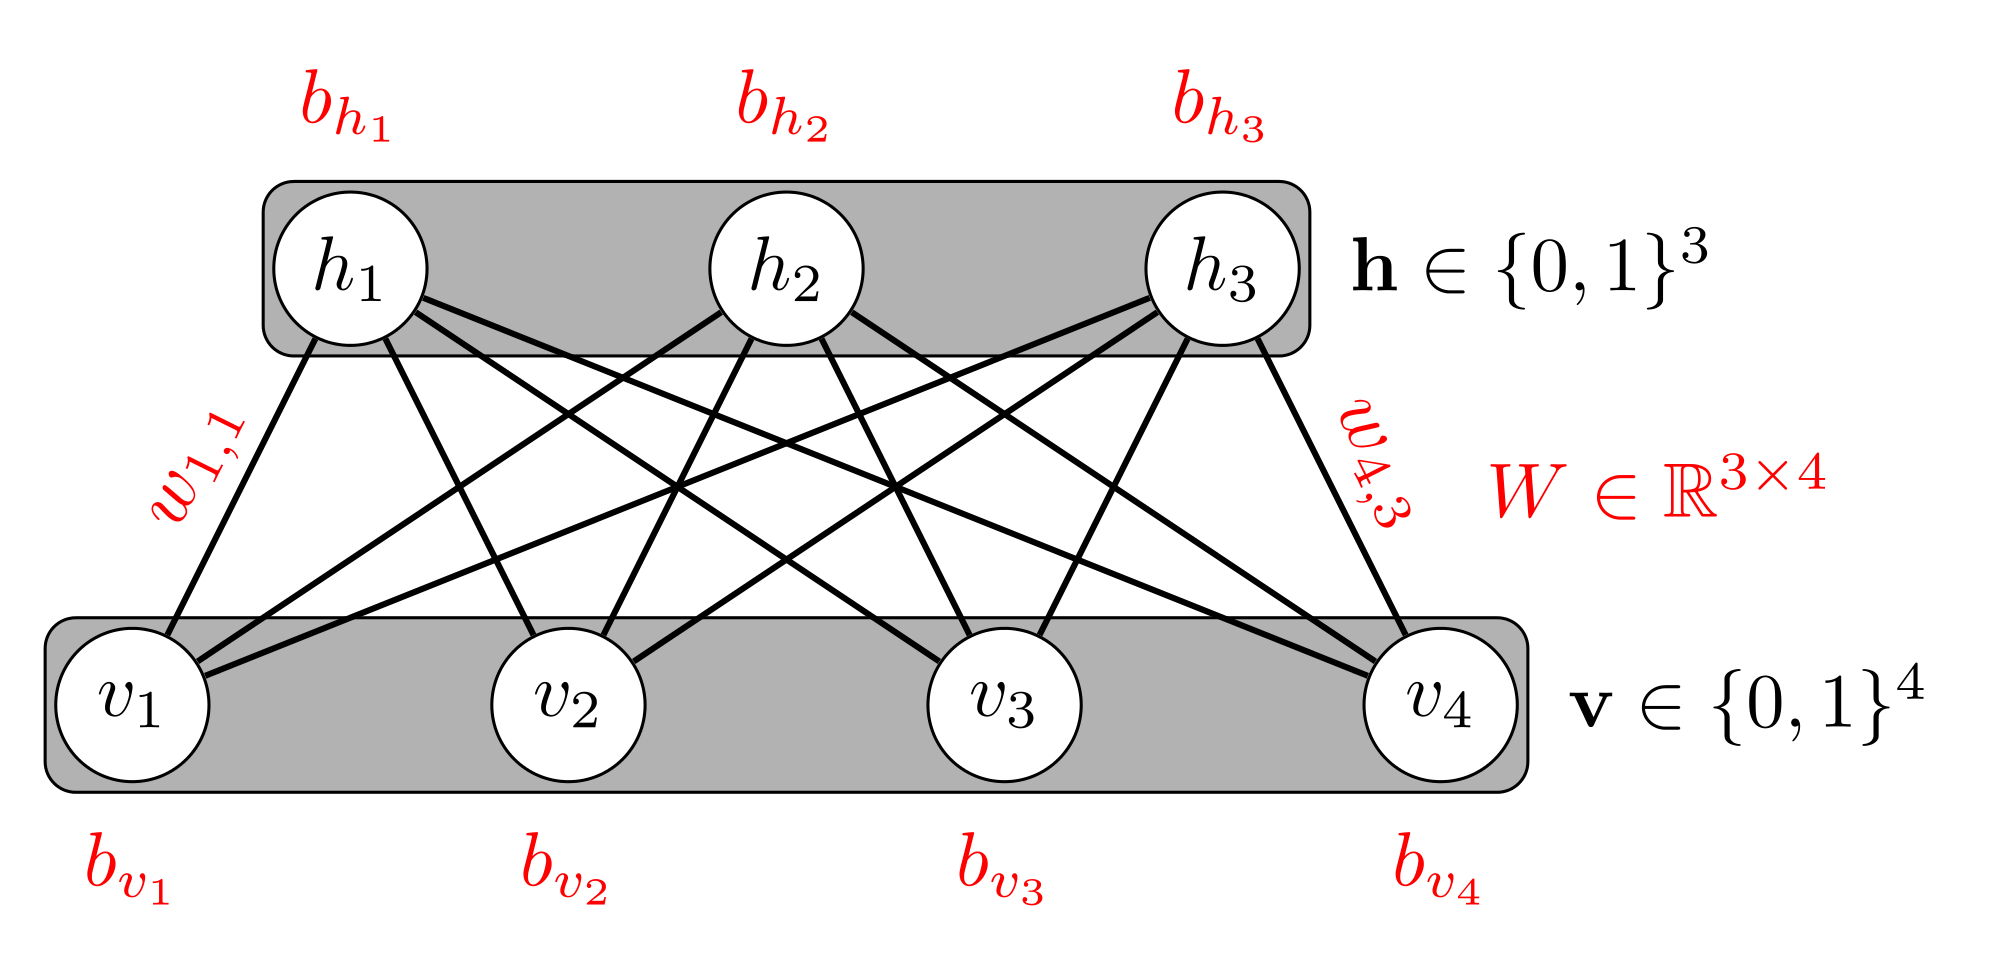
\includegraphics[width=0.45\textwidth]{figures/rbm.png}
    \caption{Restricted Boltzmann Machine.
        Figure courtesy of https://commons.wikimedia.org/wiki/File:Restricted-boltzmann-machine.svg}
    \label{Fig:RBMArchitecture}
\end{figure}

\fi

\subsection{Autoencoders}
An autoencoder is an unsupervised neural network with one hidden layer that sets the output layer to be equal to the input.
However, to prevent the network from learning the meaningless identity function, we have to place extra constraints on the network,
which generates different flavors of autoencoders.
The sparse autoencoder works by placing a sparsity constraint on the activities of the hidden neurons~\cite{SparseAE}.

We build a sparse autoencoder and our implementation is different from the
self-taught learning approaches, which also adopts the sparse autoencoder as the unsupervised feature learner~\cite{STL-NIDS, SparseAE}.
In those work, the hidden features learned by the sparse autoencoders are used directly by a classifier (e.g., a softmax regressor or an SVM).
The functionality of autoencoder resembles a transformation of a raw dataset (e.g., using principal component analysis) with the goal of obtaining a new feature space beneficial to general supervised learning algorithms.

We initialize the first layer weights of an MLP in the same way of using an RBM.
The size of the over-complete hidden layer in the sparse autoencoder is 800; the sparsity value $\rho$ is 0.05.
The autoencoder is trained with ADADELTA~\cite{ADADELTA} for 160 epochs with a batch size of 80.
We then create a separate MLP with the same configuration described in Section~\ref{CDL:SubSec:MLP},
and initialize its first layer weights with the learned weights of the autoencoder.
We use the SGD optimizer with a tiny initial learning rate 0.004
and decaying 1e-6 over each update to fine-tune the MLP model.

\iffalse
An autoencoder neural network is an unsupervised model with typically one hidden layer that
tries to set the output layer to be equal to the input.
As shown in Figure~\ref{Fig:AEArchitecture}, we want the network to
learn a function $h_{W, b}(x) \approx x$.
However, to prevent the network from learning the meaningless identity function,
we need to place extra constraints on the network, giving birth to different
flavors of autoencoders.
In this project we consider one of the most popular types of autoencoder, sparse autoencoder.

\begin{figure}[h]
    \centering
    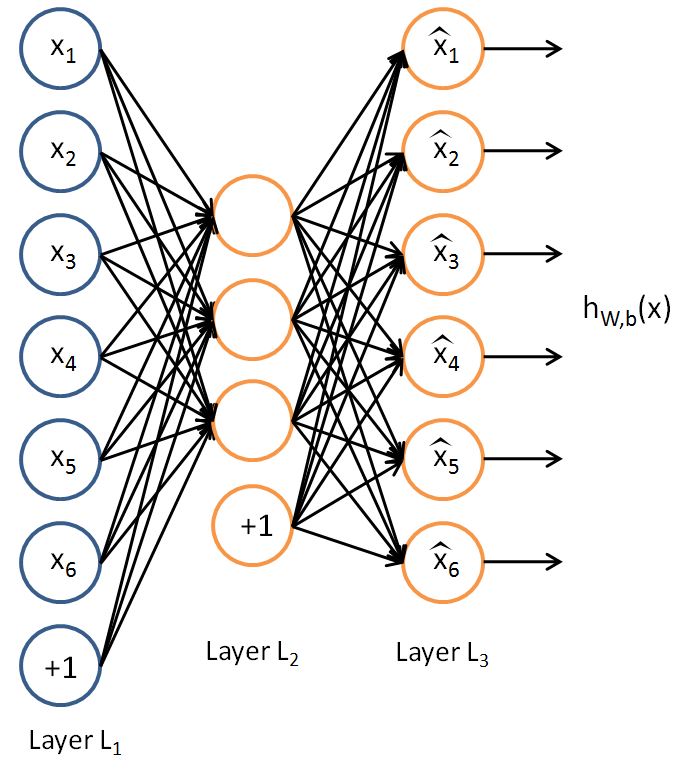
\includegraphics[width=0.45\textwidth]{figures/autoencoder.png}
    \caption{General Architecture of Autoencoders.
        Figure courtesy of~\cite{UFLDLAutoencoder}.}
    \label{Fig:AEArchitecture}
\end{figure}

The \textbf{denoising autoencoder} algorithm is proposed by~\cite{DenoiseAE} and illustrated in
Figure~\ref{Fig:dAEAlgorithm}.
To prevent learning identity function, an example $\mathbf{x}$ is first corrupted, either by
adding Gaussian noise or by random masking a fraction of items in $\mathbf{x}$ to zero.
The autoencoder then maps corrupted $\mathbf{\tilde{x}}$ to a hidden representation $\mathbf{y} = sigmoid(\mathbf{W}\tilde{\mathbf{x}} + \mathbf{b})$.
From $\mathbf{y}$ we reconstruct $\mathbf{z}=g_\theta'(\mathbf{y})$.
The training needs to learn the parameters $\theta$ and $\theta'$ so that
average reconstruction error is minimized over training set.
For binary input $\mathbf{x}$, usually cross entropy is adopted as $L_H(\mathbf{x}, \mathbf{z})$;
while mean squared error is used for real-valued $\mathbf{x}$.

Denoising autoencoder and sparse autoencoder, surprisingly, have different application domains.
Vincent et al.~\cite{DenoiseAE} have shown that stacked denoising autoencoder can be used to
initialize a deep neural network's weight parameter,
achieving similar and sometimes better performance than stacked RBM.
They also show that training stacked denoising autoencoder with MNIST dataset, it is able
to re-synthesize a variety of similarly good quality digits.
Raina et al.~\cite{SparseAE} have compared sparse encoding with principle component analysis
(PCA) and argue that transferring raw features with a well unsupervised trained
sparse autoencoder can be beneficial to supervised learning algorithms,
for example support vector machines (SVM).
\begin{figure}[h]
    \centering
    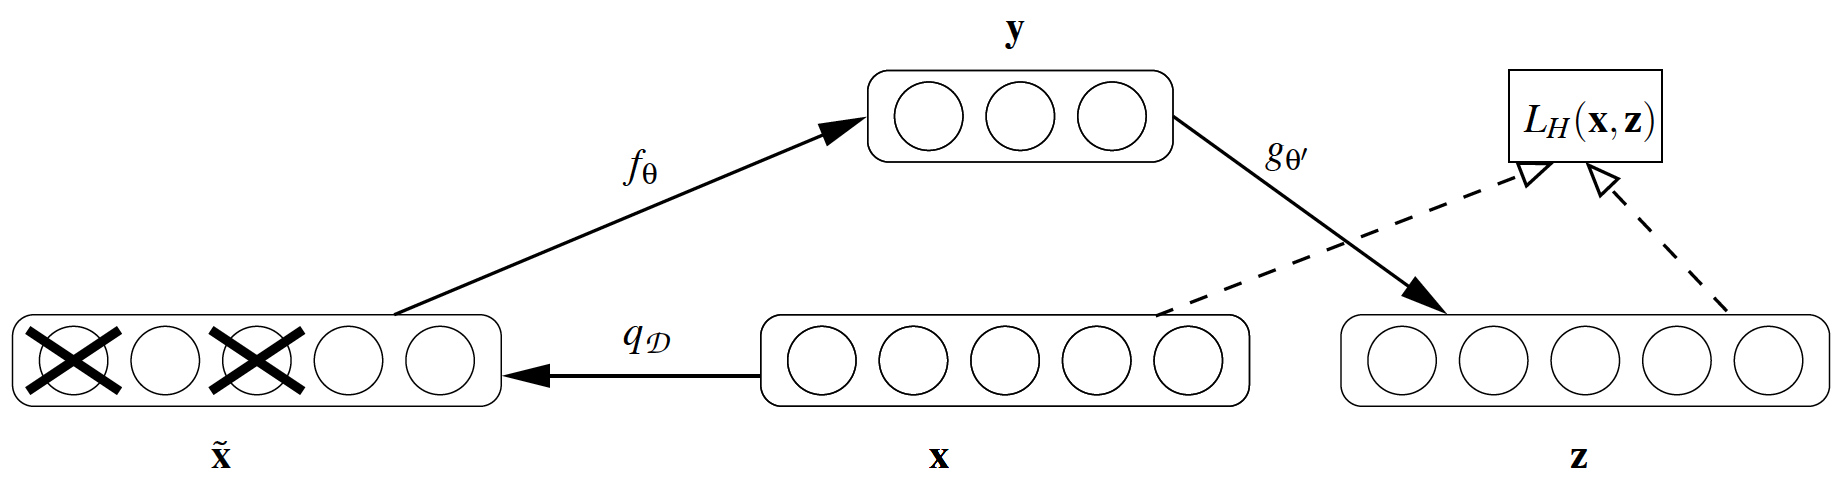
\includegraphics[width=0.45\textwidth]{figures/denoiseautoencoder.png}
        \caption{The denoising autoencoder algorithm.
        Input example $\mathbf{x}$ is randomly corrupted via $q_\mathcal{D}$ and then
        is mapped via encoder $f_\theta$ to $\mathbf{y}$.
        The decoder $g_\theta'$ attempts to reconstruct $\mathbf{x}$ and produces $\mathbf{z}$.
        Reconstruction error is measured by loss $L_H(\mathbf{x}, \mathbf{z})$, to be minimized
        during the training phase.
        Figure courtesy of~\cite{DenoiseAE}.}
    \label{Fig:dAEAlgorithm}
\end{figure}

The \textbf{sparse autoencoder} works by placing a sparsity constraint on the hidden units~\cite{SparseAE}.
First, we make the autoencoder's hidden layer size to be over-complete,
that is, of larger size comparing to the dimension of the input.
Let's denote the activation of hidden unit $j$ of layer 2 in Figure~\ref{Fig:AEArchitecture}
to be $a^2_j(\mathbf{x})$ given input example $\mathbf{x}$.
With that, we define the average activation of hidden unit $j$ over the $m$-size
training set
\begin{align}
    \hat{\rho}_j = \frac{1}{m} \sum_{i=1}^{m} a^2_j(\mathbf{x})
\end{align}
The sparsity constraint is enforcing, $\forall$ hidden unit $j$,
\begin{align}
    \hat{\rho}_j = \rho
\end{align}
where $\rho$ is a sparsity parameter that approximates zero (say 0.05).
This constraint can be vectorized over the hidden layer, say of size $n_2$,
with the KL divergence based penalty term
\begin{align}
    \sum_j^{n_2} KL(\rho || \hat{\rho}_j)
    = \sum_j^{n_2} [\rho \log \frac{\rho}{\hat{\rho}_j} + (1 - \rho) \log \frac{1-\rho}{1-\hat{\rho}_j} ]
\end{align}
The sparsity penalty term is integrated into the cost function by adding another hyper-parameter $\beta$
\begin{align}
    L(W, b) = \frac{1}{2}||h_{W,b}(\mathbf{x}) - \mathbf{x}||^2 +
    \beta \sum_j^{n_2} KL(\rho || \hat{\rho}_j)
\end{align}
\fi

\iffalse
\subsection{Generative Adversarial Nets}
As another generative model, Generative Adversarial Nets (GAN)\cite{GAN} adopts a novel training framework,
in which two models are trained simultaneously and adversarially.
The generative model $G(z;\theta_g)$ aims to capture the probability distribution of the available unlabelled dataset,
where its input is a noise variable $z$ following a prior distribution $p_z$.
The discriminative model $D(x;\theta_d)$ output the probability distribution that whether the its input source $S$ comes
from training dataset ($x\sim data$) or the generative model ($x \sim G(z)$):
\begin{align}
    D(X) = P(S|X)
\end{align}

Models $G$ and $D$ can be as simple as multilayer perceptrons,
or as complex as deep convolutional nets when the task domain is image.
The two models are trained in opposition to one another, with respect to the following log-likelihood function

\begin{align}
    V(D, G) & = \mathbb{E}_{\bm{x}\sim data} [\log P(S=real|X=\bm{x})] + \mathbb{E}_{\bm{x}\sim G(\bm{z})} [\log P(S=fake|X=\bm{x})] \\
        & = \mathbb{E}[\log D(\bm{x})] + \mathbb{E}[\log (1 - D(G(\bm{z})))]
\end{align}

With $V(D, G)$ properly defined, the training procedure is a two-player minimax game.
First we maximize the log-likelihood that $D$ correctly recognize
both the training examples and the samples generated from $G$;
in the following phase, we train $G$ to generate samples that trick $D$ to make most mistakes.
This two-phase min-max optimization can be summarized as:
\begin{align}
    \min_G \max_D V(D, G)
\end{align}

Powerful though GAN is, large amount of efforts and care are needed during training.
One way to make the training stable and fast is to augment GAN with an auxiliary classifier so that
the training phase employs the labels available in the dataset~\cite{AC-GAN}.
In auxiliary classifier GAN (AC-GAN), the discriminator $D$ now gives both the probability
distribution over the sources (whether $\bm{x}$ is real or fake) and the probability distribution
over the class labels:
\begin{align}
    D(X) = P(S|X), P(C|X)
\end{align}
Accordingly, the log-likelihood function $V(D, G)$ is augmented with the log-likelihood of the correct class $L_C$:

\begin{align} 
    V(D, G) &= L_S + L_C \\
    L_S &= \mathbb{E}_{\bm{x} \sim data} [\log P(S=real|X=\bm{x})] + 
    \mathbb{E}_{\bm{x} \sim G(\bm{z})} [\log P(S=fake|X=\bm{x})] \\
    L_C &= \mathbb{E}_{\bm{x} \sim data}[\log P(C=c|X=\bm{x})] + 
    \mathbb{E}_{\bm{x} \sim G(\bm{z})} [\log P(C=c|X=\bm{x})]
\end{align}

The training procedure for AC-GAN is similar to GAN: we train $D$ to maximize $V(D, G)$;
while at the same time we train $G$ to minimize $L_S - L_C$.
Currently, we are interested in using GAN or AC-GAN to generate fake traffic.
In the future, we will also attempt the semi-supervised classification framework with AC-GAN.
\fi

\subsection{Wide and Deep Learning with Embeddings}
\label{SubSec:WD}
The categorical and integer features are extremely sparse in the network intrusion datasets.
%For illustration reason, we plot the histogram of the ``dloss" integer feature in UNSW-NB15 dataset,
%which denotes the number of destination packets retransmitted or dropped.
%As shown in~\ref{Fig:DlossHist}, ``dloss"'s values range from 0 to 6000, while more than 97\%
%of the occurred value is 0 but values from 1000 to 6000 do appear in the dataset.
For example, a categorical feature ``proto" indicates one of the 133 protocol types that a traffic record belongs to. Therefore, one-hot encoding will generate a 133-dimension vector consisting only one field with the value one. Neural networks are often not good at utilizing sparse large dimension inputs.
We tackle this problem in two ways concerning the combined model in~\cite{WideDeepModel}.
The first solution is to embed the integer or categorical features.
An embedding is a mapping from sparse discrete objects to a dense vector of real numbers.
``word2vec" is widely used in the natural language processing and machine translation tasks, where embeddings are treated as points in the vector space so that the similarity between objects can be visually measured
by the Euclidean distance or angle between the vectors.
In this case, embedding provides a solution to converting large-vocabulary-size categorical features and sparse integer features to dense vectors of continuous values.
Deep neural network fed with embedding inputs can generalize better even with less feature engineering.
As stated in~\cite{WideDeepModel}, these input features to the deep neural nets are denoted as deep components consisting of continuous and embedded features.
Second, we leverage some simple linear models with nonlinear feature transformations to address the sparse inputs. The method is called wide components~\cite{WideDeepModel}, which consists of the basis and crossed features.
The basis features are the raw input features that are either integer or categorical.
The crossed features are the cross-product transformations of basis features that memorize the interactions between raw features.
The Wide and Deep model complements a deep neural network
with embedded low-dimension input vectors for good generalization.
Its linear sub-model is integrated with the deep neural network using a weighted sum of each model's output for good memorization.

The wide and deep learning model requires engineering the raw attributes in datasets into basis, crossed, continuous, and embedded components.
In our implementation, the basis features are all the raw symbolic and integer attributes.
Crossed features are built by a subset of combinations of the symbolic attributes in a dataset.
The raw symbolic and integer attributes are fed to the deep neural network as embedded components after conducting embedding.
The continuous components are the raw continuous attributes.
To compare with other models, we set the structure of the deep neural network in the wide and deep model to be the same sizes as the baseline MLP, i.e., two hidden layers with the size of [800 480].

\iffalse
\begin{align}
    \Phi_k (\bm{x} ) = \prod_{i=1}^{d} {x_i}^{c_{ki}}
\end{align}
where
\begin{align}
    c_{ki} = 
    \begin{cases}
        1, & \text{$i$-th feature $\in$ the transformation $\Phi_k$} \\
        0, & \text{otherwise}
    \end{cases}
\end{align}

\begin{align}
    \Phi_k (\mathbf{x} ) = \prod_{i=1}^{d} {x_i}^{c_{ki}}, \text{ where }
    c_{ki} = 
    \begin{cases}
        1, & \text{$i$-th feature $\in \Phi_k$} \\
        0, & \text{otherwise}
    \end{cases}
\end{align}
The function of wide components, especially the cross-product transformations,
is memoization of the raw feature interactions.
\begin{figure*}[h]
    \centering
    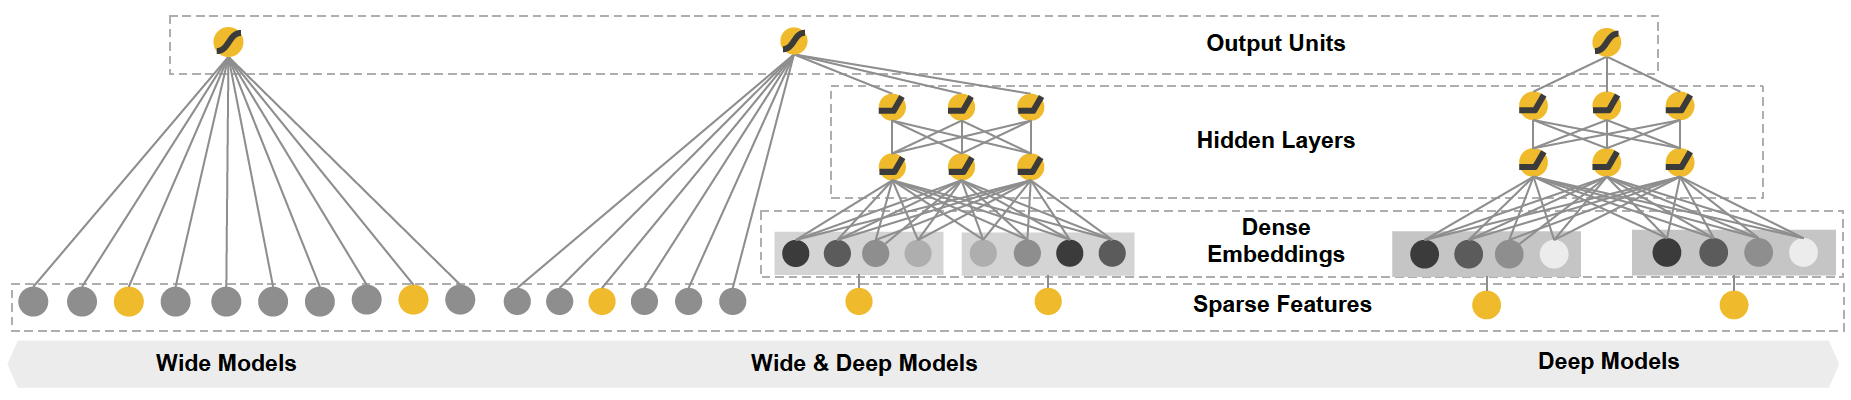
\includegraphics[width=0.98\textwidth]{figures/WideDeepModel.png}
    \caption{Anatomy of Wide and Deep Model}
    \label{Fig:WideDeepModel}
\end{figure*}

\begin{figure}[h]
    \centering
    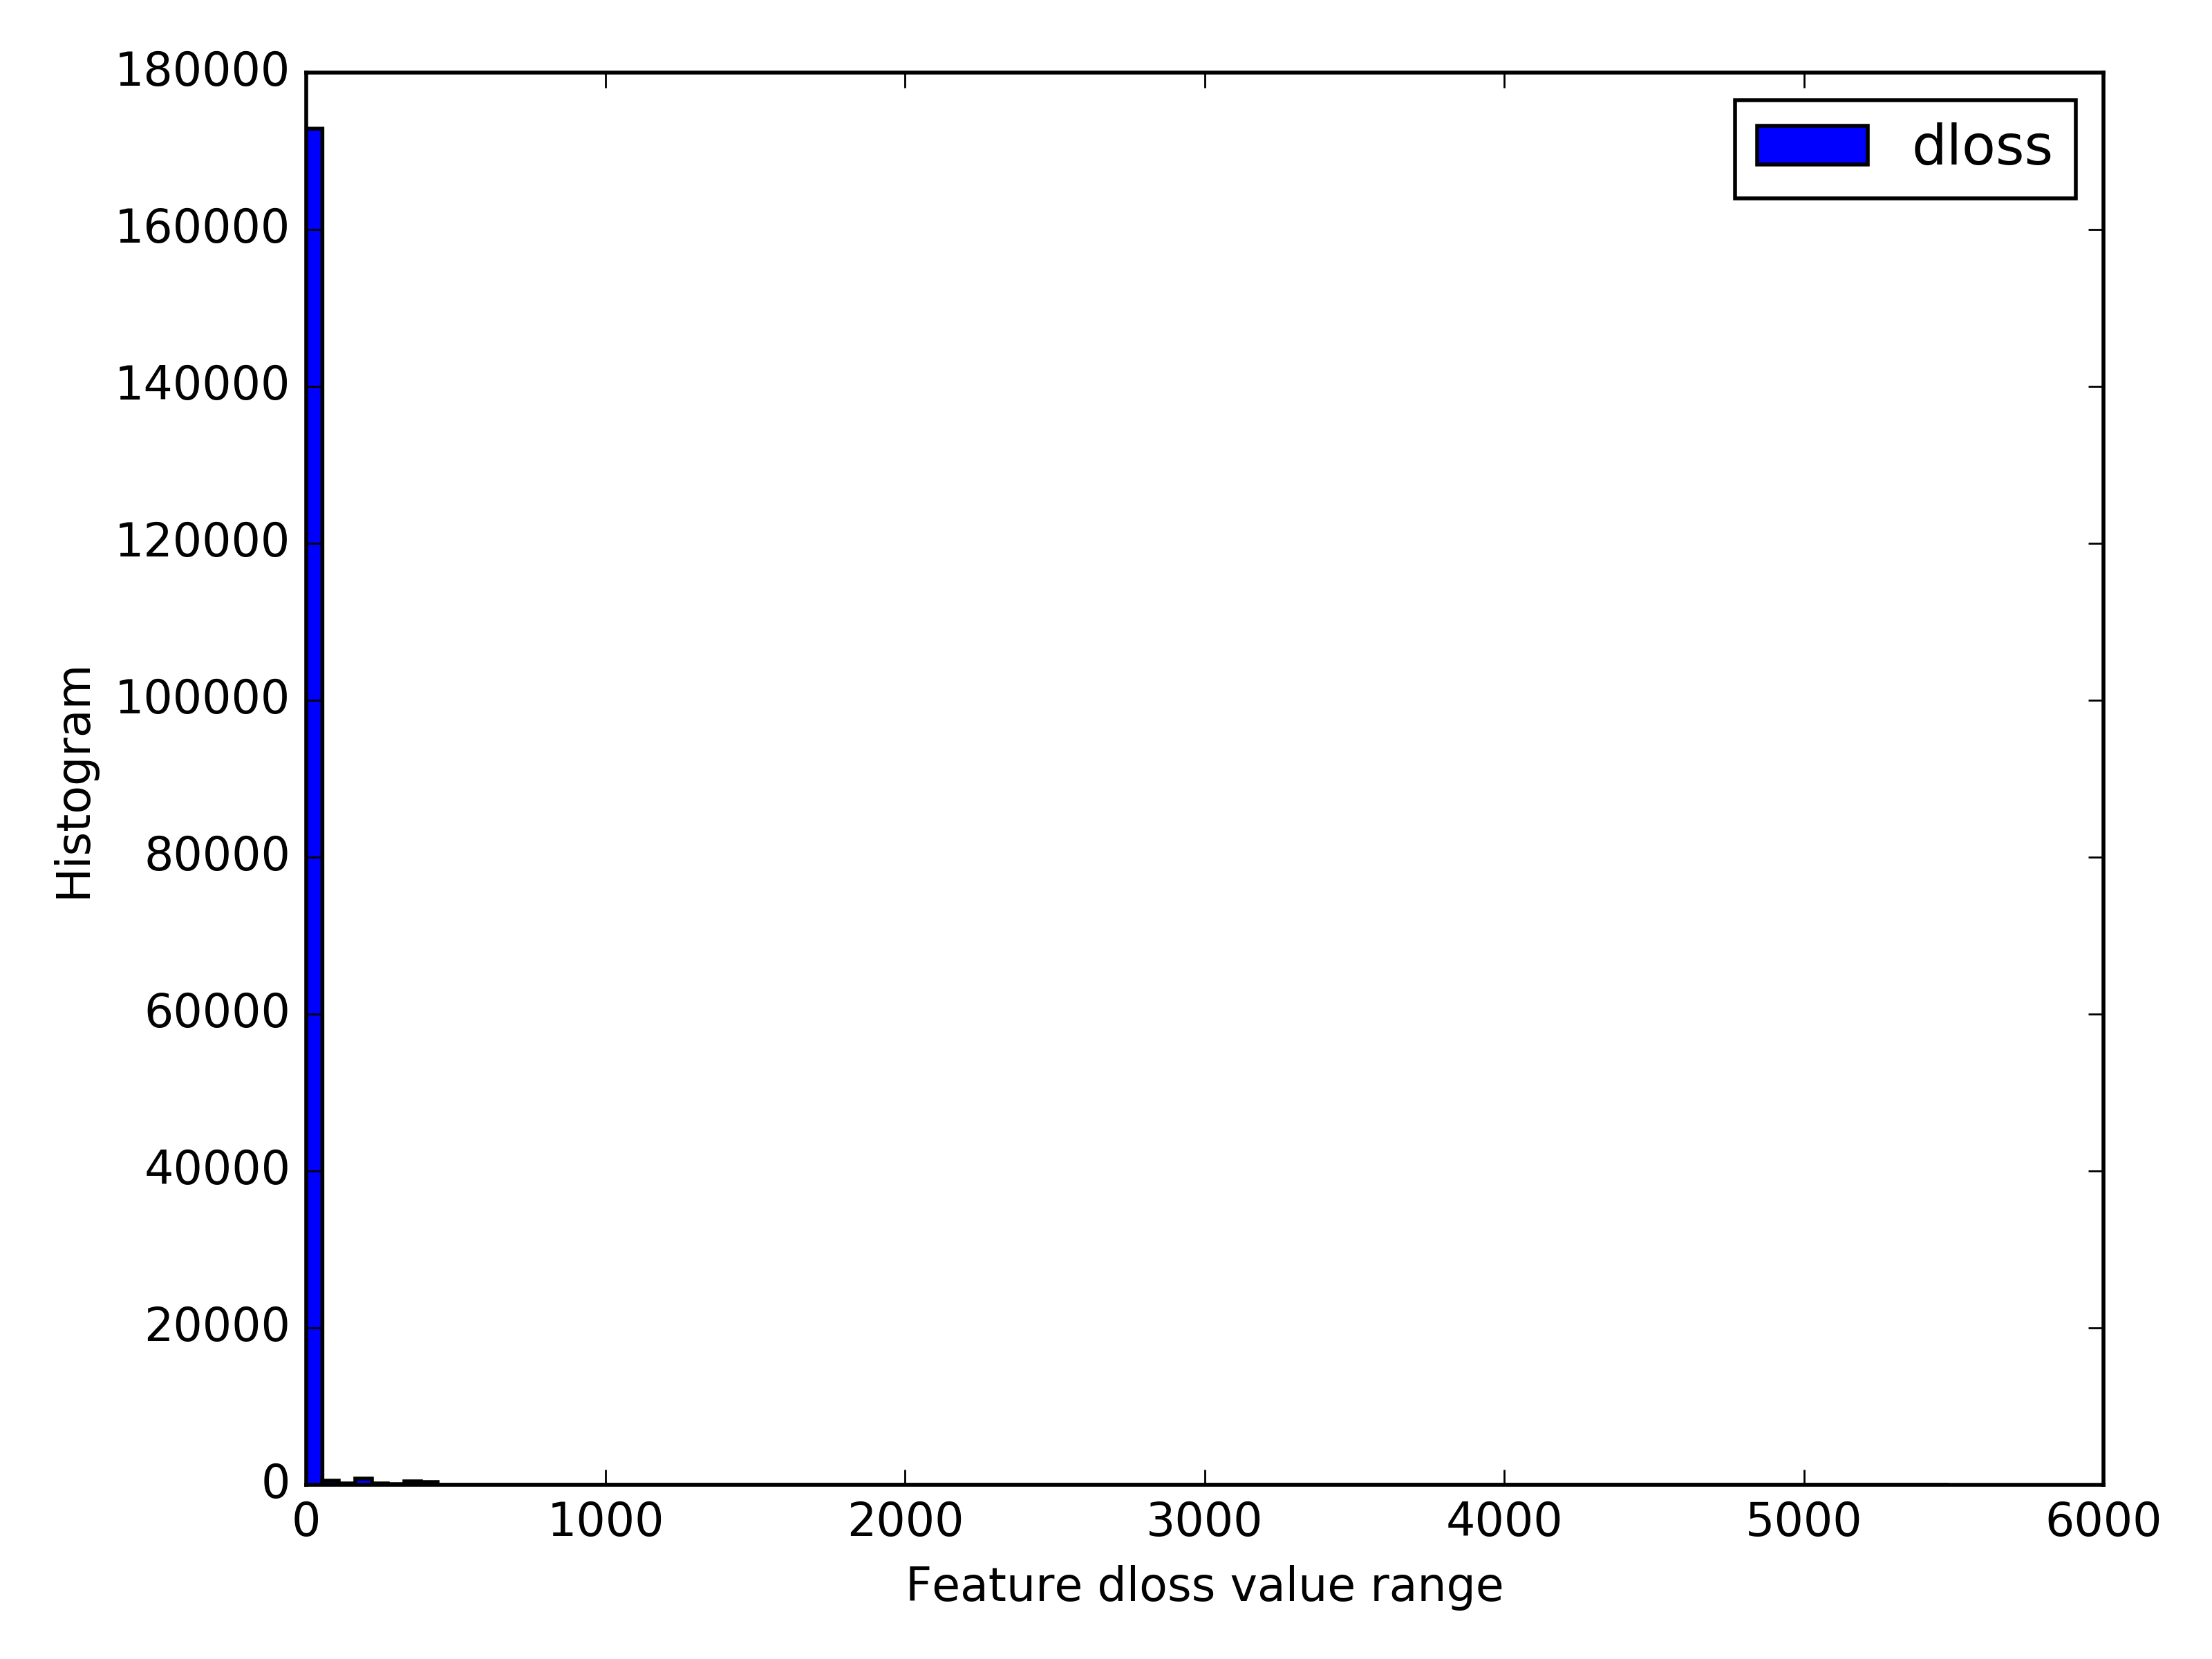
\includegraphics[width=0.45\textwidth]{figures/dloss_hist.png}
    \caption{Histogram of the Feature ``dloss" from UNSW-NB15 Dataset.}
    \label{Fig:DlossHist}
\end{figure}
\fi

\section{Experimental Evaluation}

We evaluate all the models developed in NetLearner on the 5-class NSL-KDD task and the 2-class UNSW-NB15 task using the following metrics.
\begin{itemize}
    \item \textbf{Accuracy} is the percentage of correctly classified connections
        over the total number of connections in the dataset:
        \begin{align}
            A = \frac{\text{True Positives + True Negatives}}{\text{Number of Instances}}
        \end{align} 
        Accuracy is not suitable for evaluating imbalance datasets where the number
        of records of one class is extremely larger than the number of
        records of another class.
        In the NSL-KDD dataset, the number of available U2R records (i.e., 67)
        is two orders of magnitude less than the number of records in other classes
        (i.e., 9711, 7458, 2887 and 2121).
        Therefore, we also consider the precision and recall.
    \item \textbf{Precision} is the percentage of the correctly classified positives over
        the total number of positives predicted by the classifier.
                \begin{align}
                    P = \frac{\text{True Positives}}{\text{True Positives} + \text{False Positives}}
                \end{align}
    \item \textbf{Recall} is the percentage of the correctly classified positives over
                the total number of relevant elements.
                \begin{align}
                    R = \frac{\text{True Positives}}{\text{True Positives} + \text{False Negatives}}
                \end{align}
\end{itemize}
%The weight for each class is determined by its proportion in the test dataset,
%namely [0.431, 0.107, 0.339, 0.018, 0.105] for class [Normal, Probe, DoS, U2R, R2L] respectively.
%Besides, we also calculate the confusion matrices of the classification results when applying
%different approaches on both task's test datasets.
%In a confusion matrix table, the $i$th row represents the instances of class $i$,
%while the $j$th column represents the instances predicted by the classifier as class $j$.
%It is called confusion matrix because it is useful for visualizing how a classifier
%is confusing one class with other classes.
%Due to page space limit, here we only present the most straightforward
%and relatively more important metric accuracy.
%Statistics regarding precision, recall and confusion matrices can be found
%in our detailed technical report~\cite{OurWonReport} and our codebase~\cite{NetLearner}.

We train an radial basis function kernel support vector machine (SVM) % using the approach in ~\cite{ScikitLearnSVM},
and report its accuracy with the multilayer perceptron (MLP) model,
the restricted Boltzmann machine fine-tuned neural network (RBM),
the sparse autoencoder fine-tuned neural network (SAE),
and the wide linear classifier and deep neural network combined model (WnD).

It is critical to search the optimal hyper-parameters that fit the problem domain and model before training machine learning models. We first manually set all the hyper-parameters, including the number of layers, number of neurons in each layer, learning rate, and batch size, to be identical across all the models.
We then use 5-fold cross-validation on the training datasets to determine the optimal training time $T$
for each model.
Finally, we train the model for $T$ epochs and report the metrics on the testing dataset,
which is not touched during the training phase.
Determining the training time (model complexity) by cross-validation with fixed common hyper-parameters
ensures that the deep learning models are neither overfitting nor underfitting.
We plot the 5-fold cross validation loss of MLP in Figure~\ref{CDL:Fig:LossHistory}.
We can see that the validation loss converges to approximately 0.02 after 140 epochs, even though the training loss still decreases,
and the optimal training time that validation loss is minimized is at $T \approx 150$.
In this case, we train the MLP on NSL-KDD train dataset for exactly 150 epochs and report its metrics on NSL-KDD test dataset.

The accuracies of all considered classifier are shown in Figure~\ref{CDL:Fig:CompAccuracyNSL} for the NSL-KDD task and
Figure~\ref{CDL:Fig:CompAccuracyUNSW} for the UNSW-NB15 task.
In the 2-class UNSW-NB15 dataset,
the volumes of normal and attacking traffic are nearly balanced (i.e., 37,000 normal v.s. 45,332 attacking records).
Therefore, we only report the precision and recall for the attacking traffics in Figure~\ref{CDL:Fig:CompAccuracyUNSW}.
For the 5-class NSL-KDD task, we adopt the approach in~\cite{STL-NIDS}
to calculate the weighted precisions and recalls, and plot them together with accuracy in Figure~\ref{CDL:Fig:CompAccuracyNSL}.
The per-class precisions and recalls are also listed in Table~\ref{CDL:Tab:PrecisionRecall}.

For the NSL-KDD task, all classifiers achieve high training accuracy (no less than 99\%).
However, all classifiers show a gap between training accuracy and testing accuracy (as low as 78.4\%).
As the representative of the classic machine learning approach, SVM achieves a 78.5\% accuracy
comparable to the deep learning models.
Note that our SAE model achieves the same accuracy performance to~\cite{STL-NIDS}, which is the best among all the considered models (79.2\%).
RBM, SAE, and WnD all outperform MLP for two different reasons.
RBM and SAE provide their underlying MLP with better initial weights in the first layer
than randomly generated numbers.
WnD has a slightly higher accuracy because of the extra linear model.
Table~\ref{CDL:Tab:PrecisionRecall} shows two remarkable facts.
SVM performs better at Probe attacks (93\% precision and 82\% recall)
than all the neural networks ($\approx$ 85\% precision and $\leq$ 70\% recall),
However, it suffers hugely on U2R attacks ($\approx$ 6\% precision and recall).
On the other hand, the neural networks (MLP, RBM, SAE and WnD) miss many U2R attacks ($\leq$ 6\% recall),
but they have much higher reliability in identifying these attacking traffic ($\approx$ 60\% precision).

For the UNSW-NB15 task, the average accuracies of RBM, SAE and WnD are
all higher than MLP for the same reason mentioned in the NSL-KDD task.
We notice WnD has significantly improved MLP's performance by around 5\%.
Different from the NSL-KDD task, the training accuracies of all the approaches are mediocre
(up to 94.4\%) in contrast to the NSL-KDD case where the training accuracy of every model is more than 99\%.
The harder UNSW-NB15 training dataset is one primary reason that the testing accuracies of the UNSW-NB15 task
are higher than that of the NSL-KDD task, since classifiers only have access to the training dataset.
Therefore, even though SVM has an equivalent training accuracy to the neural networks (93\% v.s. 94\%),
its testing accuracy falls far behind by 5\% (comparing to MLP) to 9\% (comparing to WnD),
showing the superior generalization capability of the deep neural network models.
The detection alarms are mostly correct for every classifier,
due to the high recall values $\geq$ 97\%, and the deep learning models have better precision ($\geq$ 81\%) than SVM (75\%).

\begin{figure}[h]
    \centering
    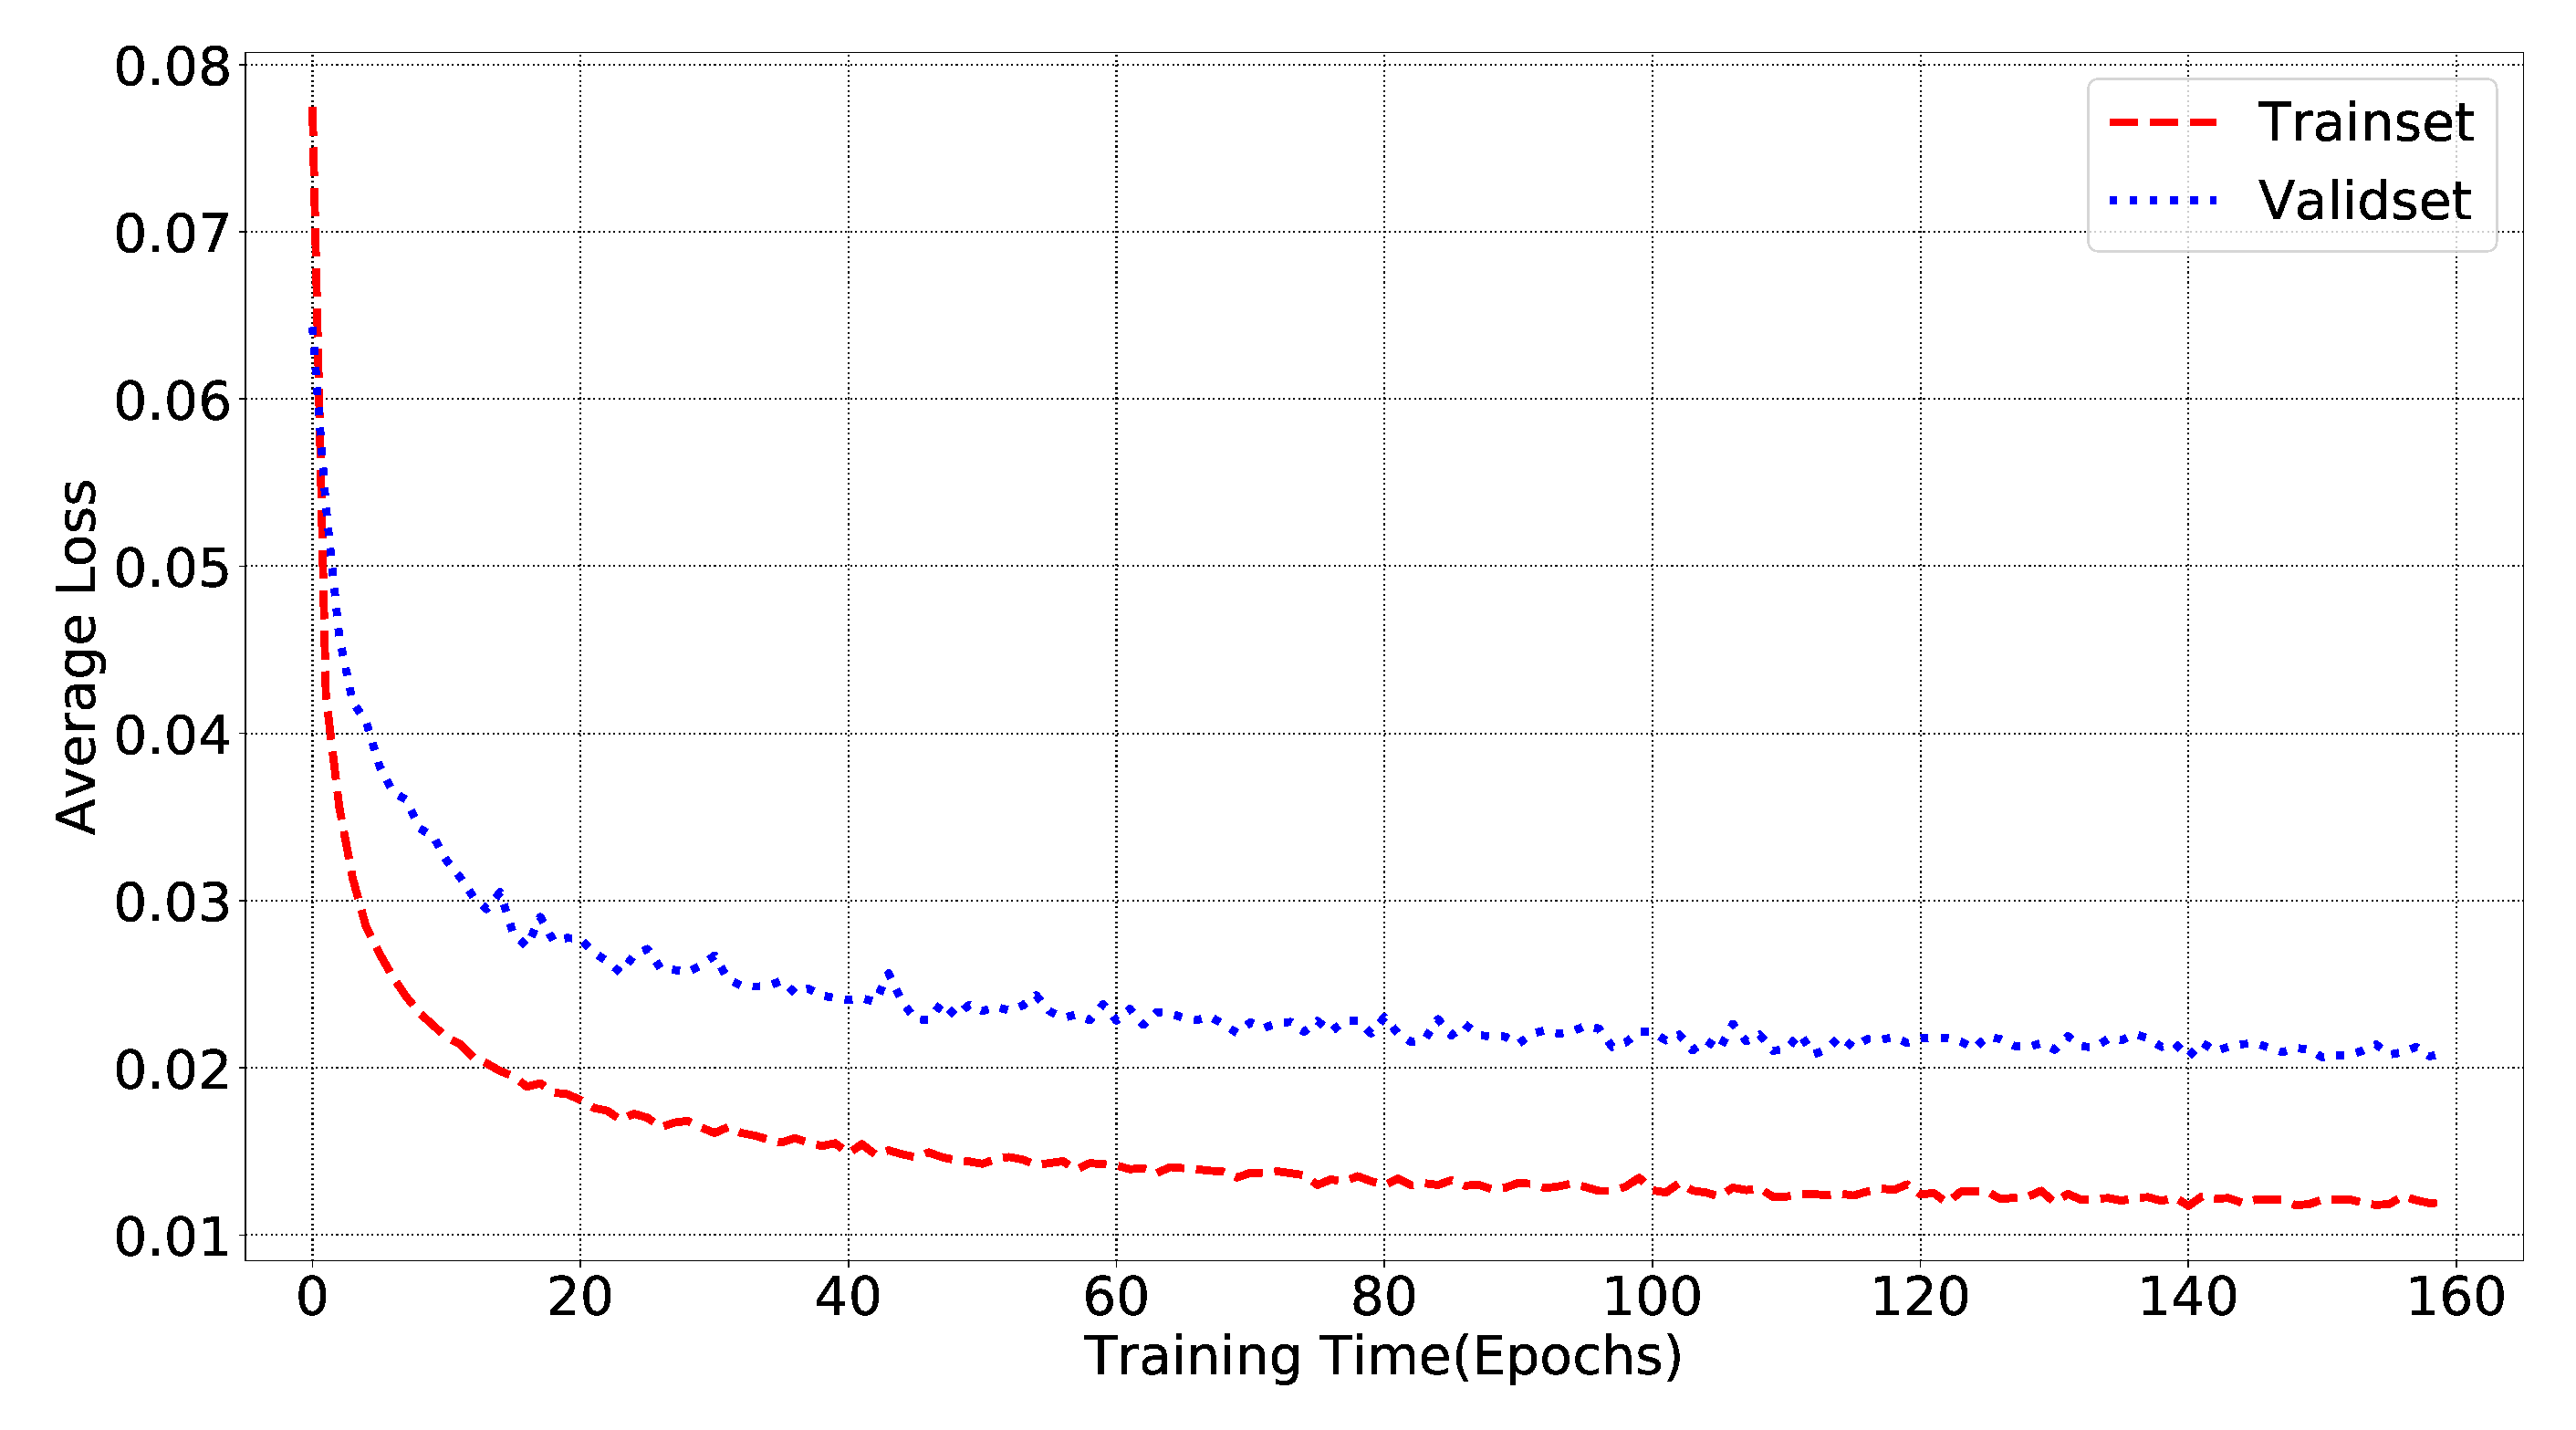
\includegraphics[width=0.9\textwidth]{CompareDL/figures/history.eps}
    \caption{History of MLP's Average Loss During Cross Validation}
    \label{CDL:Fig:LossHistory}
\end{figure}

\begin{figure}[h]
    \centering
    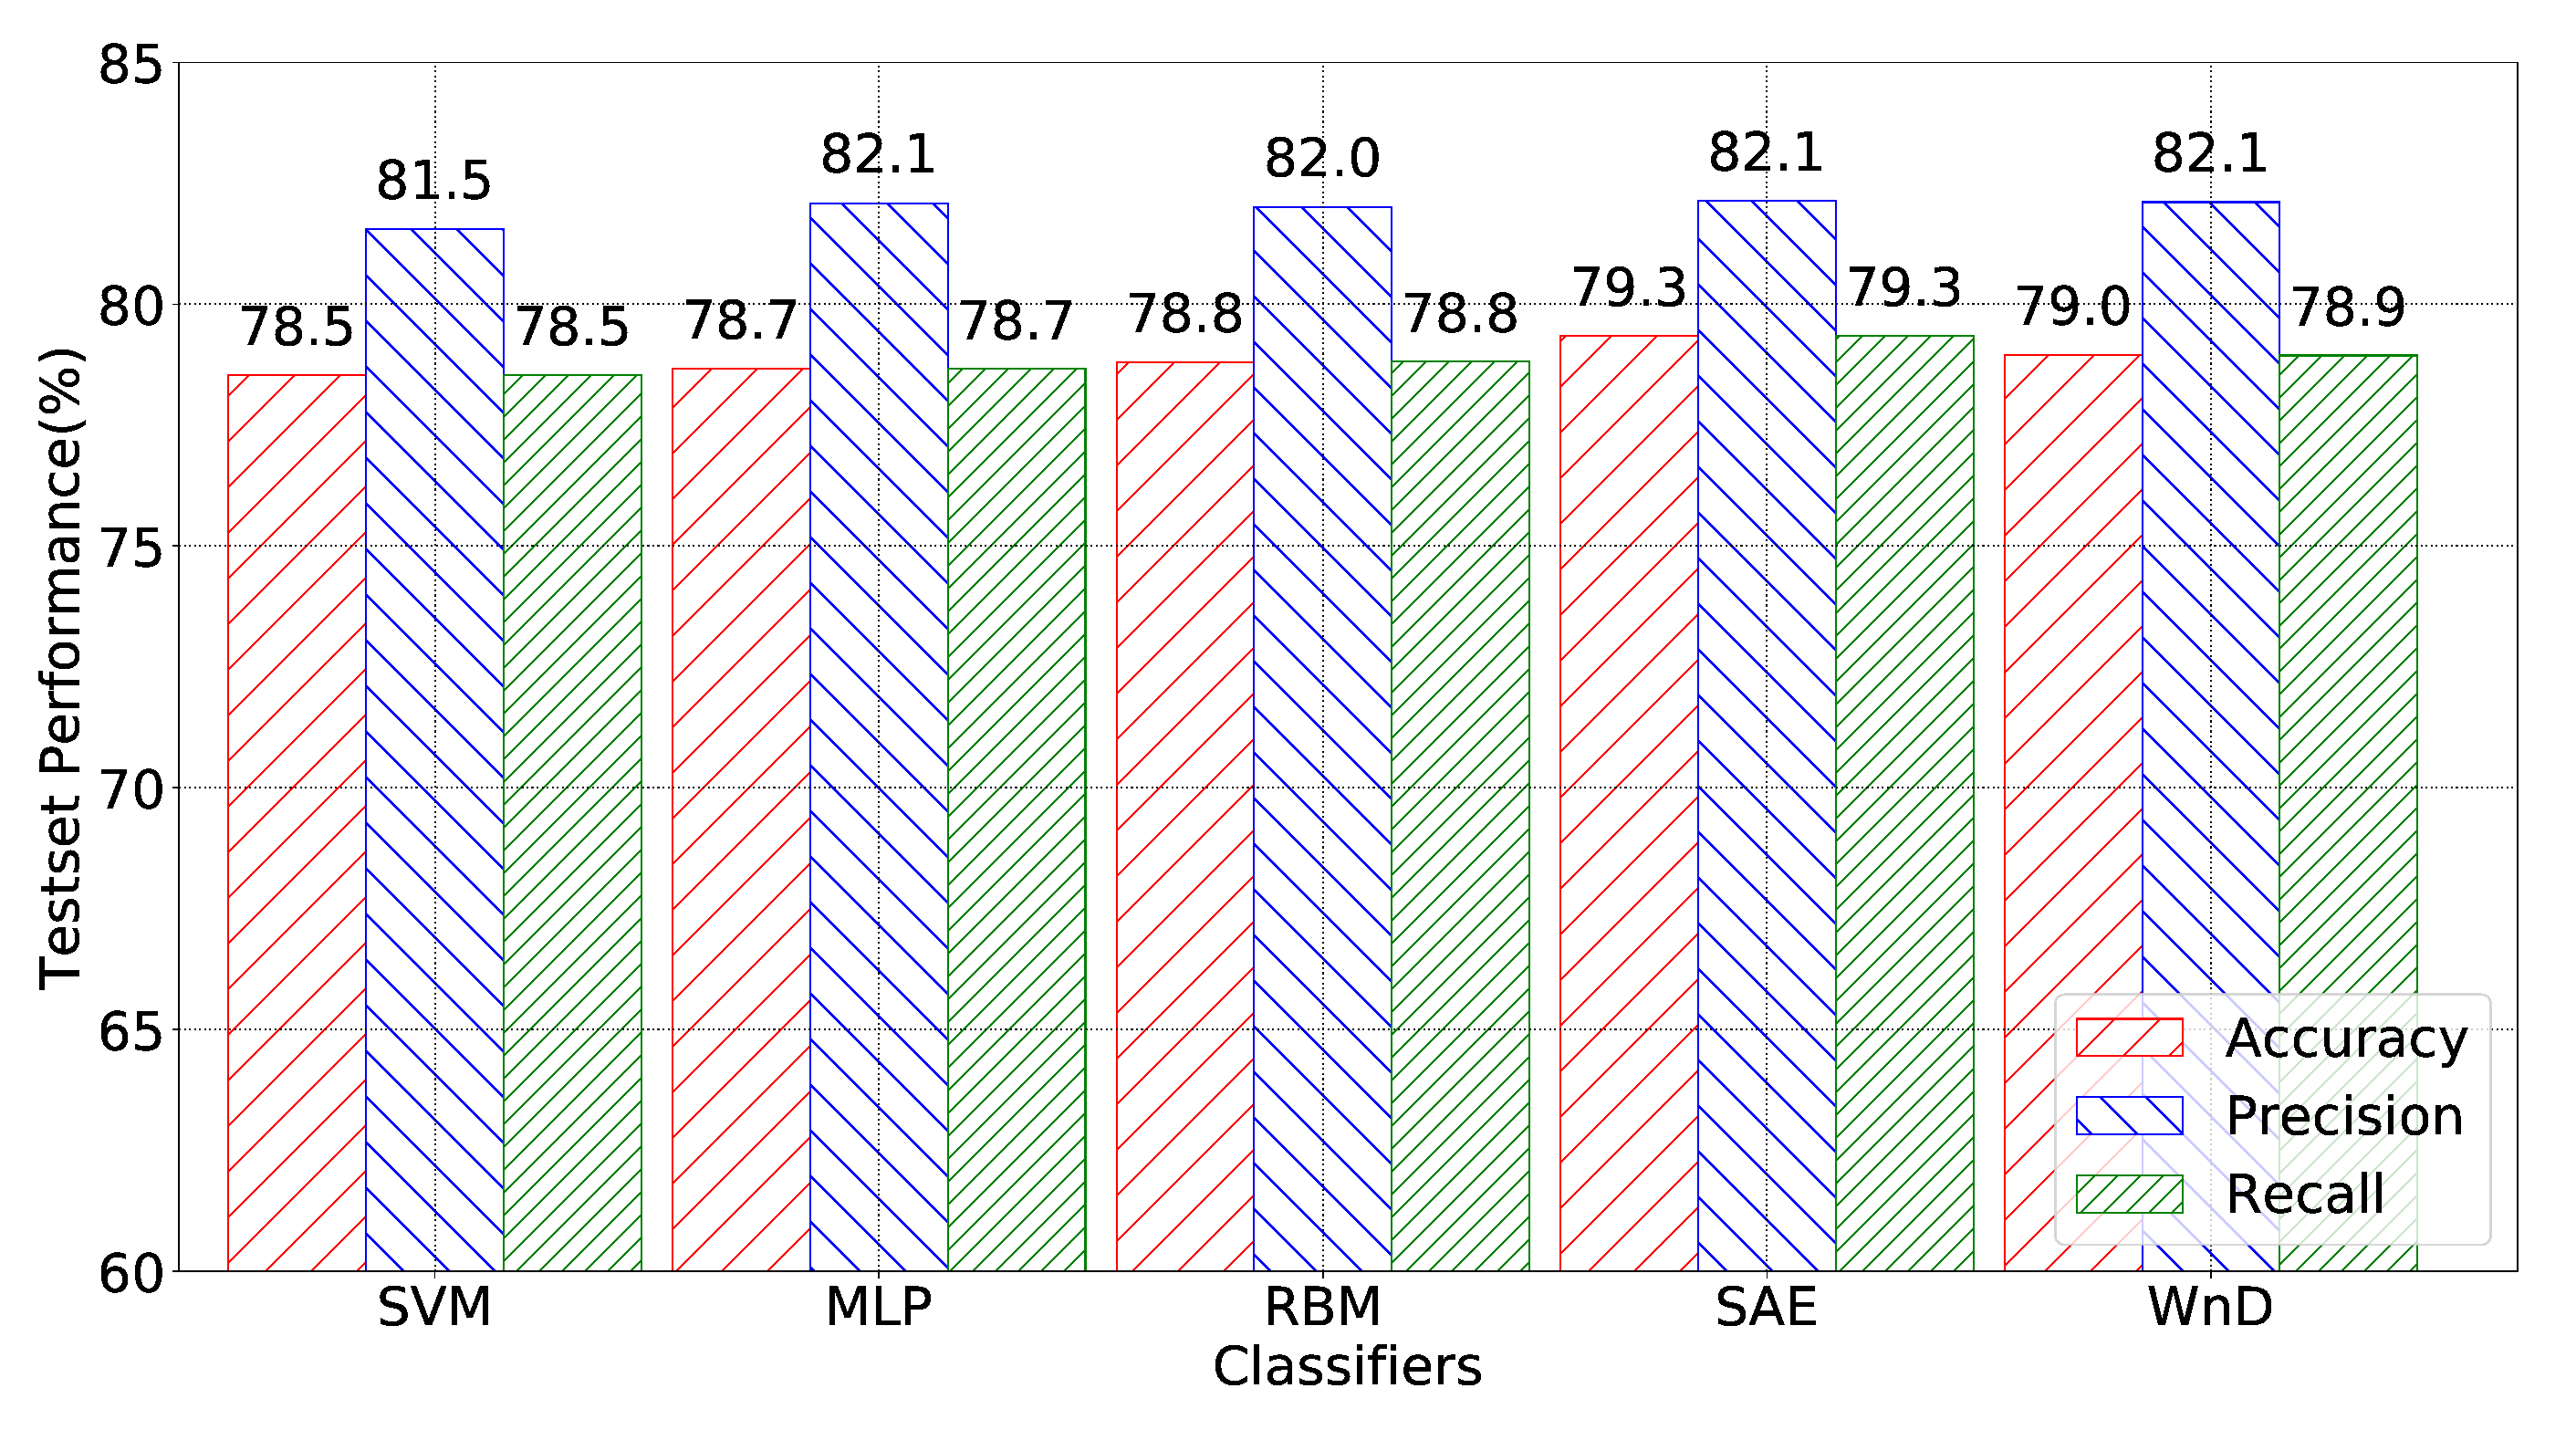
\includegraphics[width=0.9\textwidth]{CompareDL/figures/comp_accuracy_nsl.eps}
    \caption{Metrics Comparison, NSL-KDD Task}
    \label{CDL:Fig:CompAccuracyNSL}
\end{figure}

\begin{figure}[h]
    \centering
    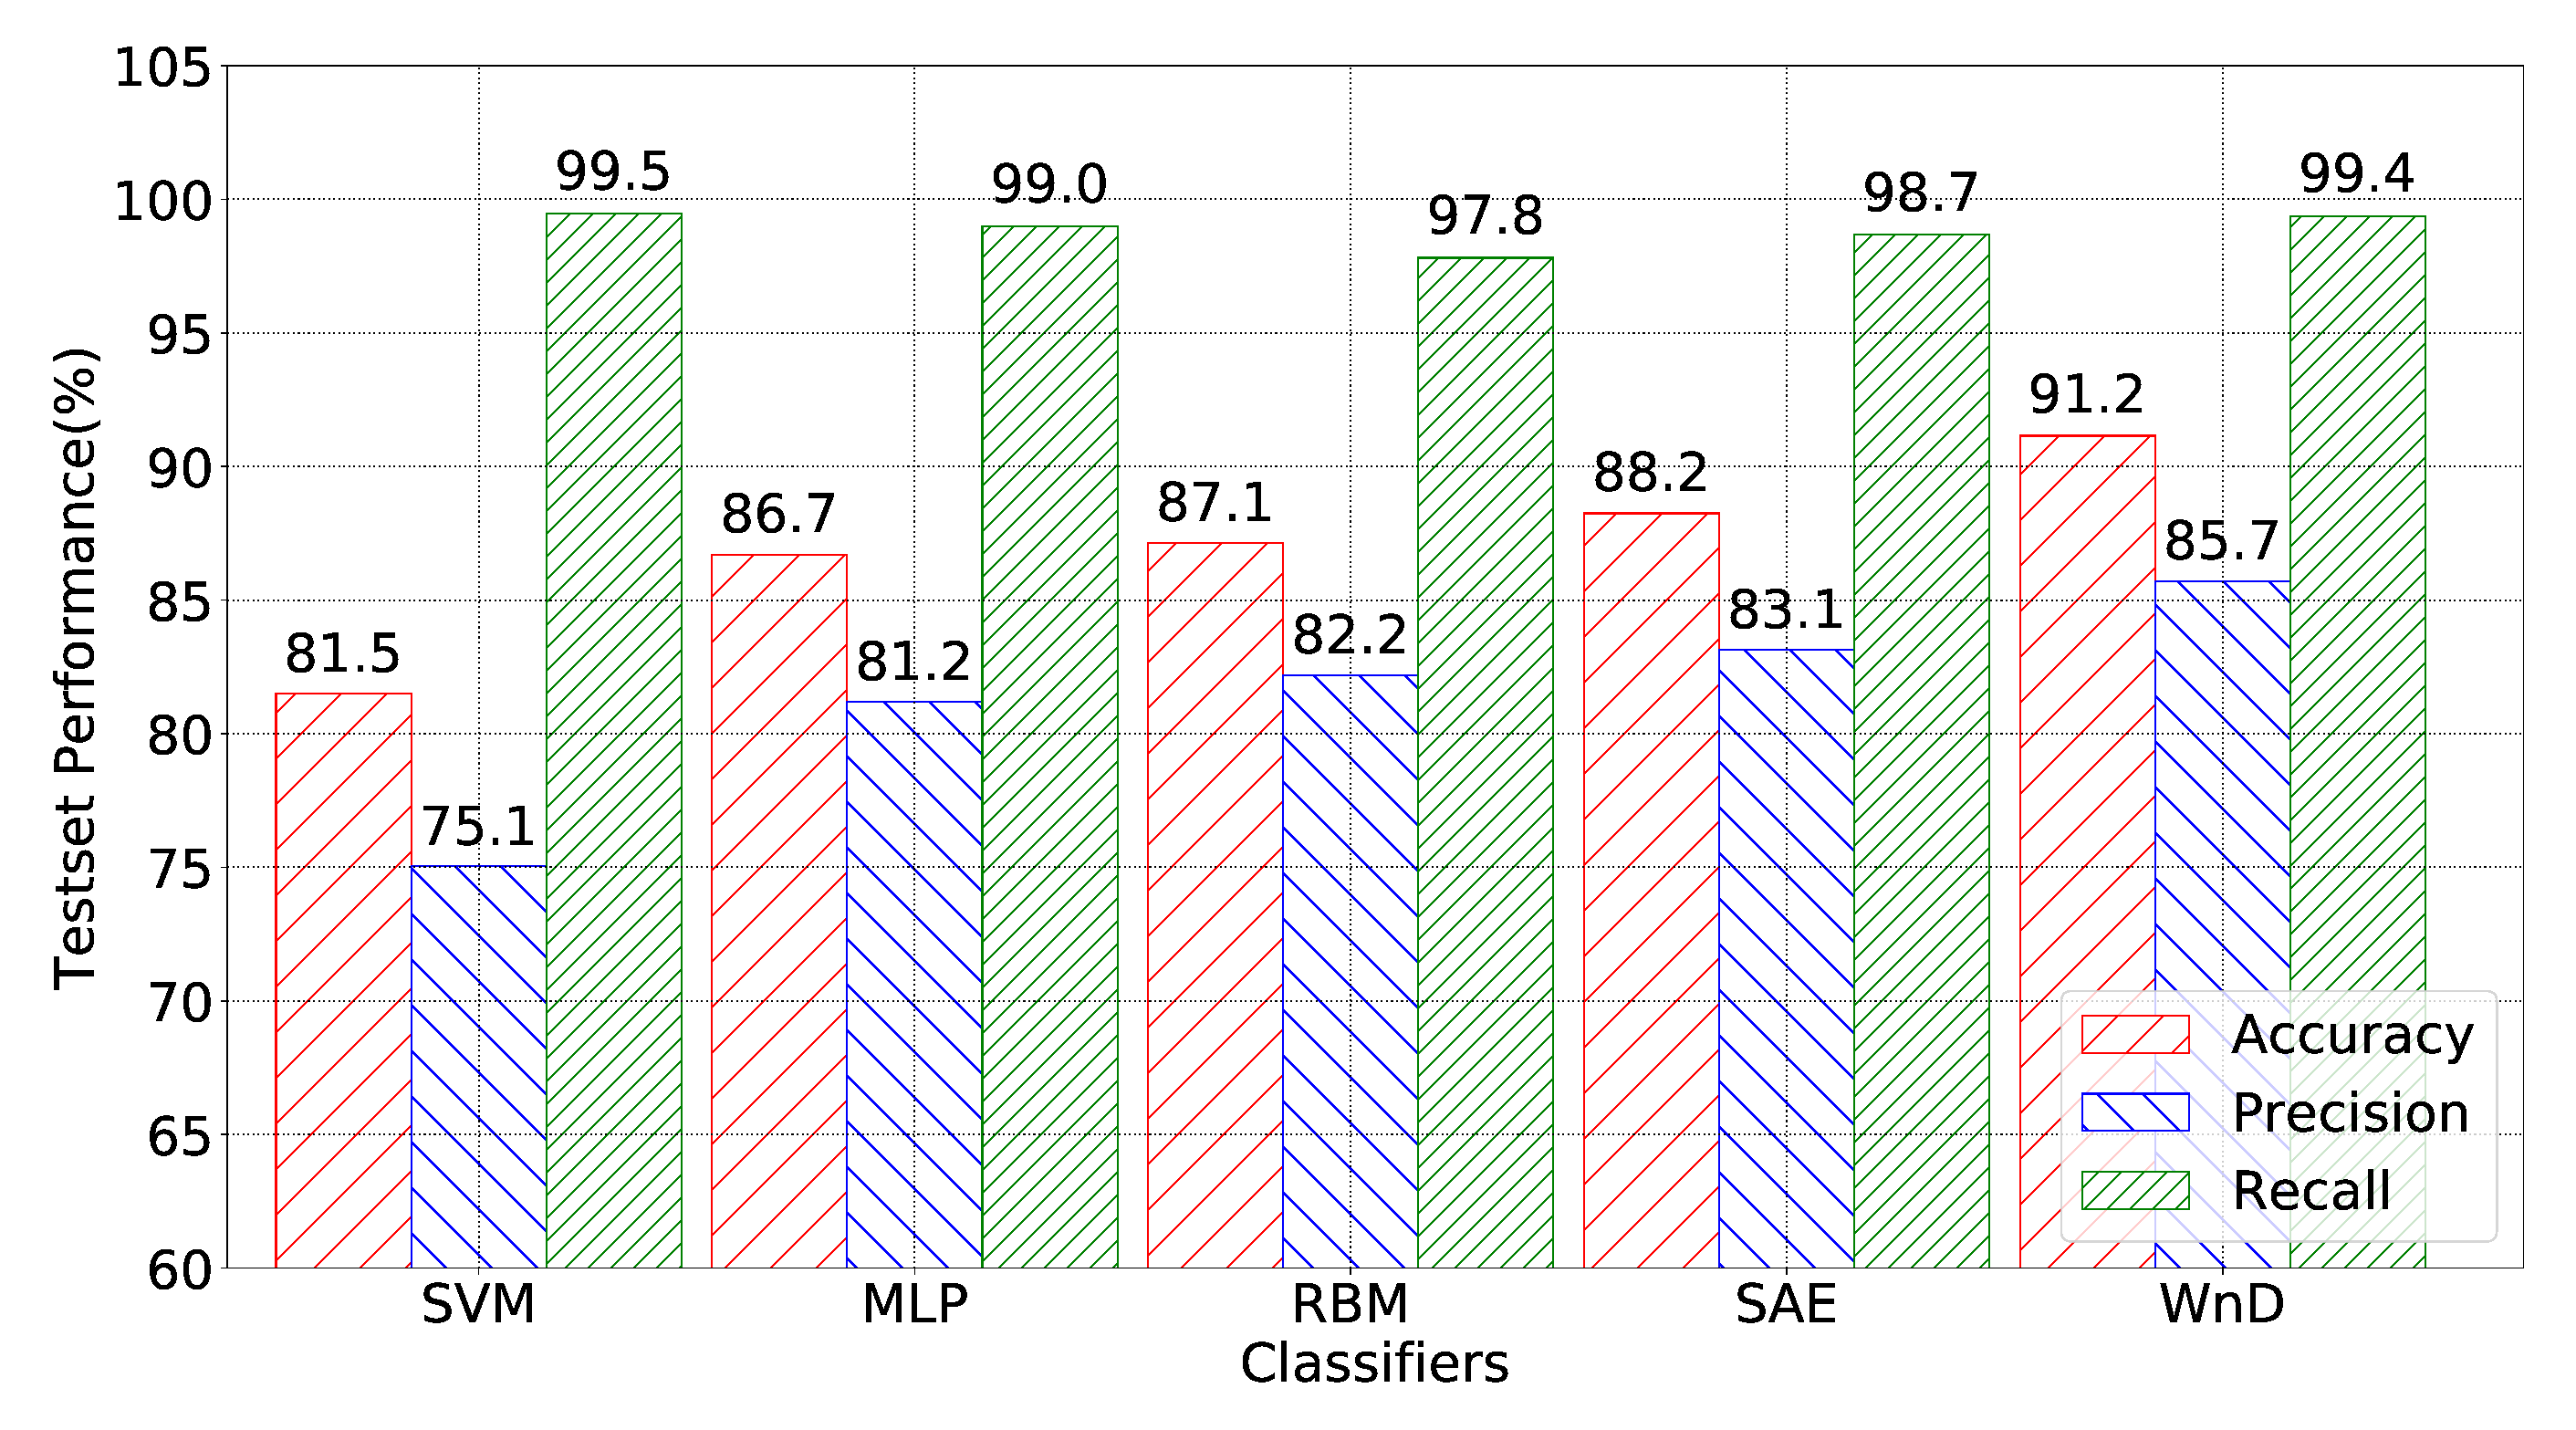
\includegraphics[width=0.9\textwidth]{CompareDL/figures/comp_accuracy_unsw.eps}
    \caption{Metrics Comparison, UNSW-NB15 Task}
    \label{CDL:Fig:CompAccuracyUNSW}
\end{figure}

\begin{table}[tbp]
    \centering
    \caption{Per-class Precision/Recall on the NSL-KDD Task}
    \label{CDL:Tab:PrecisionRecall}
    \begin{tabular}{c|c|ccccc}
        \hline
        \hline
                             &            & \multicolumn{5}{c}{Traffic Class} \\
        \cline{3-7}
                             &            & Normal & DoS   & Probe & U2R   & R2L \\
        \hline
        \multirow{2}{*}{SVM} & Precision  & 72.82  & 75.27 & 93.85 &  6.32 & 96.65 \\
        \cline{2-2}
                             & Recall     & 96.18  & 72.16 & 82.16 &  6.06 & 13.34 \\
        \hline
        \multirow{2}{*}{MLP} & Precision  & 69.18  & 95.49 & 85.58 & 59.52 & 92.01 \\
        \cline{2-2}
                             & Recall     & 96.66  & 82.31 & 69.28 &  6.31 & 15.03 \\
        \hline
        \multirow{2}{*}{RBM} & Precision  & 69.41  & 95.41 & 85.23 & 41.51 & 93.86 \\
        \cline{2-2}
                             & Recall     & 96.81  & 83.89 & 64.74 &  5.56 & 15.48 \\
        \hline
        \multirow{2}{*}{SAE} & Precision  & 70.20  & 95.63 & 84.70 & 65.00 & 87.76 \\
        \cline{2-2}
                             & Recall     & 96.92  & 83.34 & 70.56 &  3.28 & 16.29 \\
        \hline
        \multirow{2}{*}{WnD} & Precision  & 70.08  & 95.59 & 84.02 & 60.34 & 91.57 \\
        \cline{2-2}
                             & Recall     & 96.88  & 83.64 & 67.84 &  4.53 & 15.34 \\
        \hline
    \end{tabular}
\end{table}


\section{Summary of Deep Learning Based NIDS}

We study cutting-edge deep learning models to the design of network intrusion detection systems.
%First, we briefly discuss general deep learning methodology and its potential implication on the network intrusion detection problem.
%Then we describe a set of promising deep learning models in concisely mathematical languages.
With the help of our open-source Tensorflow-based deep learning library NetLearner,
we perform a comparative evaluation of those models on two network intrusion detection tasks using the NSL-KDD and UNSW-NB15 datasets.
Preliminary experimental results show that for the NSL-KDD task, sparse autoencoder achieves accuracy similar to the existing machine learning solutions;
for the UNSW-NB15 dataset, deep neural network models with greater generalization capability achieve better accuracy than SVM based solutions.

\clearpage

\Chapter{Deep Learning for Malware Classification}
\label{Cpt:DLMC}
\section{System Overview of \sysname}
\label{MG:Sec:System}

%Before that, let's take an overview of the components in \sysname in the pipeline order.
This section overviews the three main components of \sysname, whose workflow is illustrated in Figure~\ref{fig:SystemPipeline}.

\begin{figure*}[htbp]
\centerline{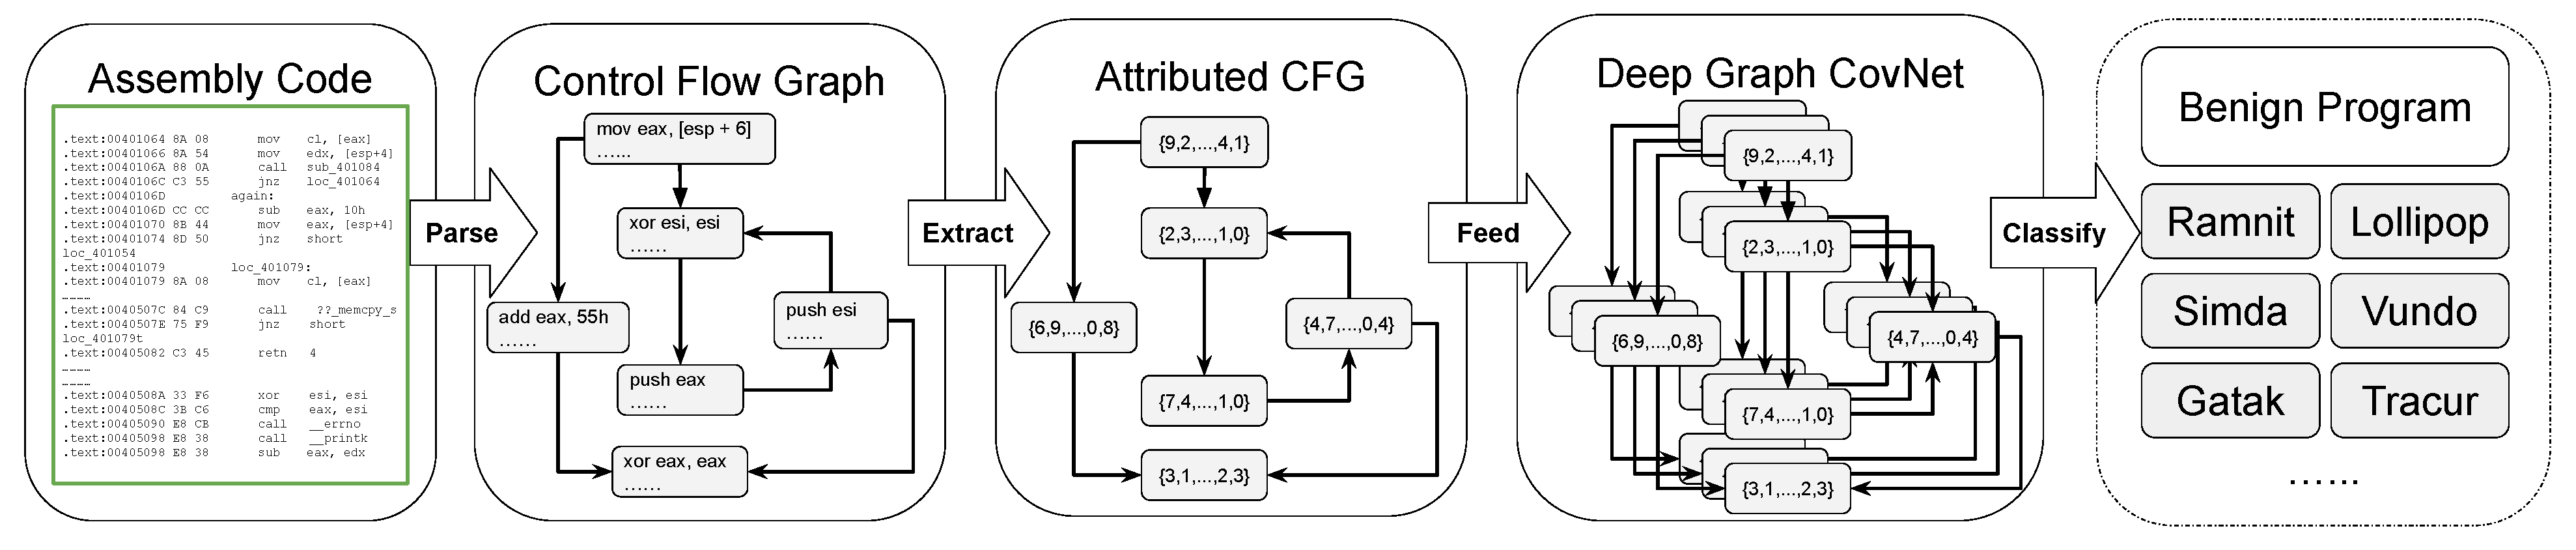
\includegraphics[width=1.0\textwidth]{Magic/figures/SystemPipeline.eps}}
\caption{The workflow of \sysname, a DGCNN-based malware classification system}
\label{fig:SystemPipeline}
\end{figure*}

\subsection{Control Flow Graph}\label{subsec:ConstructCfg}
%Given a cross-platform assembly code, 

\sysname relies on the state-of-the-art tools, such as IDA Pro~\cite{bib:idapro}, to extract CFGs from malware code.
In a CFG, a vertex represents a basic block, which contains a straight sequence of code or assembly instructions without any control flow transition except at its exit.
Two vertices $(u, v)$ are connected by a directed edge $u \rightarrow v$ if either the last instruction in $u$ falls through the first line of code in $v$,
or there is a jump instruction in $u$ that is destined to some instructions (e.g., jump target) in $v$.
The implementation details on how to build the CFG from disassembled execution code will be given in Section~\ref{sec:BuildCfg}.

\subsection{Attributed Control Flow Graph}\label{subsec:Cfg2Acfg}
The CFG representation of software program is generic for the purpose of malware classification in several ways.
First, this type of representation transcends specific programming languages in which the programs are written or hardware platforms for which the programs are developed.
Although other low-level representations such as hexadecimal byte sequences have similar properties, a CFG explicitly expresses the execution logic of a program using a graph data structure.
Hence, the semantics of a malware program is embodied by not only the characteristics of the code in individual basic blocks but also their structural dependencies defined by the edges connecting these basic blocks. 


%which can be used as raw features us works on ML-based malware classification but also 

%The expressive power of CFGs also enables the collection of a variety of aggregate features


%Furthermore, the vertices in the graph provide us a suitable unit environment to extract code-level attributes, many of which are scatteringly adopted by existing machine learning models as raw features.

To convert CFGs to structures that are amenable to machine learning, we define attributes at each vertex that summarize code characteristics as numerical values.
Initially the attributes computed at a vertex do not contain any structural information, which means that their values are independently collected from the corresponding basic block.
Table~\ref{tab:UsedAttributes} lists the attributes implemented in our prototype system, although more attributes can be conveniently added to further improve malware classification performance.

\begin{table}[htbp]
\caption{Block-level attributes used in \sysname}
\begin{center}
\begin{tabular}{c|l}
\hline
Attribute Type & Attribute Description \\
\hline
\multirow{10}{*}{From Code Sequence} & \# Numeric Constants \\
 & \# Transfer Instructions         \\
 & \# Call Instructions             \\
 & \# Arithmetic Instructions       \\
 & \# Compare Instructions          \\
% & \# Crypto instructions           \\
 & \# Mov Instructions              \\
 & \# Termination Instructions      \\
 & \# Data Declaration Instructions \\
 & \# Total Instructions            \\
\hline
\multirow{2}{*}{From Vertex Structure} & \# Offspring, i.e., Degree \\
 & \# Instructions in the Vertex    \\
 \hline
\end{tabular}
\label{tab:UsedAttributes}
\end{center}
\end{table}

As the raw attributes in an attributed CFG (ACFG) contain little structural information and the number of vertices in an ACFG varies with the individual program from which the CFG is derived, for the purpose of malware classification it is necessary to aggregate these attributes over all the vertices in the ACFG in an organic manner depending on its graph structure.
The task of such attribute aggregation is accomplished with DGCNN, which shall be explained next.

%Figure~\ref{fig:SystemPipeline} shows how the further processing on the vertices of a CFG offers us the attributed CFG representation.

%Attributes are numeric values that characterize a vertex in a CFG.
%It usually describes the sequence of code inside a code block, such as the number of constants and the number of transfer instructions.
%It also includes structural information of the vertex, such as the number of offspring and betweenness.


\subsection{Deep Graph Convolution Neural Network}\label{subsec:DGCNN}
Unlike image or text-based data, graph-based data are of variable sizes and are thus not naturally ordered tensors.
%Therefore, a gap exists between the ACFG and the optimal features on the basis of which a machine-learning-powered detection engine makes malware prediction. In our pipeline, this gap is bridged by 
To address this challenge, we use the state-of-the-art deep neural network that can automatically learn discriminative latent features from malware data abstracted as ACFGs.
Particularly, we use deep graph convolution neural network to transform unordered graph data of varying sizes to tensors of fixed size and order.
The transformation algorithm first recursively propagates the weighted attributes in each vertex through the neighborhood defined by the graph structure.
Next, it sorts the vertices in the order of their feature descriptors.
After the sorting step, the graphs with variant sizes are embedded into fixed-size vectors, which are amenable to ML-based classification.
In the next section, we shall elaborate on these operations as well as our extensions based on formal mathematical descriptions.

\section{Algorithm Description}
\label{MG:Sec:DGCNN}

Our work on applying DGCNN for malware classification in \sysname has been inspired by the deep learning model proposed in~\cite{Dgcnn}. In this section, we first introduce how DGCNN aggregates attributes through the neighborhood defined by the graph structure. We then discuss how to extend the existing DGCNN model with our own modifications. To explain the rationale of the DGCNN-based malware classification algorithm clearly, we walk through an example graph with five vertices as shown in Figure~\ref{MG:Fig:ExampleGraph}.

\subsection{Primer on DGCNN}

\textbf{Notations.} We denote the adjacency matrix of a graph $G=(V, E)$ of $n$ vertices as $\mathbf{A} \in \mathbb{Z} ^{n\times n}$.
Note that $G$ is a directed graph, and $\mathbf{A}$ is not necessarily symmetric.
To allow the attributes of a vertex to be propagated back to the vertex itself, we define the augmented adjacency matrix $\tilde{\mathbf{A}} = \mathbf{A} + \mathbf{I}$.
Accordingly, the augmented diagonal degree matrix of $G$ is defined as $\tilde{\mathbf{D}}$, where
$\tilde{\mathbf{D}}_{i,i} = \sum_j \tilde{\mathbf{A}}_{i,j}$.
We assume that each vertex is associated with a $c$-dimension attribute vector.
Therefore, we use $\mathbf{X} \in \mathbb{R}^{n \times c}$ to denote the attribute matrix for all the vertices in the graph. %$\forall v \in V$.
Alternatively, we can also treat $\mathbf{X}$ as the concatenation of $c$ \textit{attribute channels} of the graph.
For the sample graph $g$ in Figure~\ref{MG:Fig:ExampleGraph}, we assume the vertices have two attribute channels,
and display the corresponding augmented adjacency matrix $\tilde{\mathbf{A}}$, the augmented diagonal degree matrix $\tilde{\mathbf{D}}$,
and the attribute matrix $\mathbf{X}$ with two attribute channels named $F1$ and $F2$.
Given $\tilde{\mathbf{A}}$ and $\mathbf{X}$ for graph $G$, the DGCNN-based algorithm performs three sequential stages to obtain its tensor representation for malware classification. Note that $\tilde{\mathbf{D}}$ can be calculated from $\tilde{\mathbf{A}}$.

\begin{figure*}[htbp]
\centerline{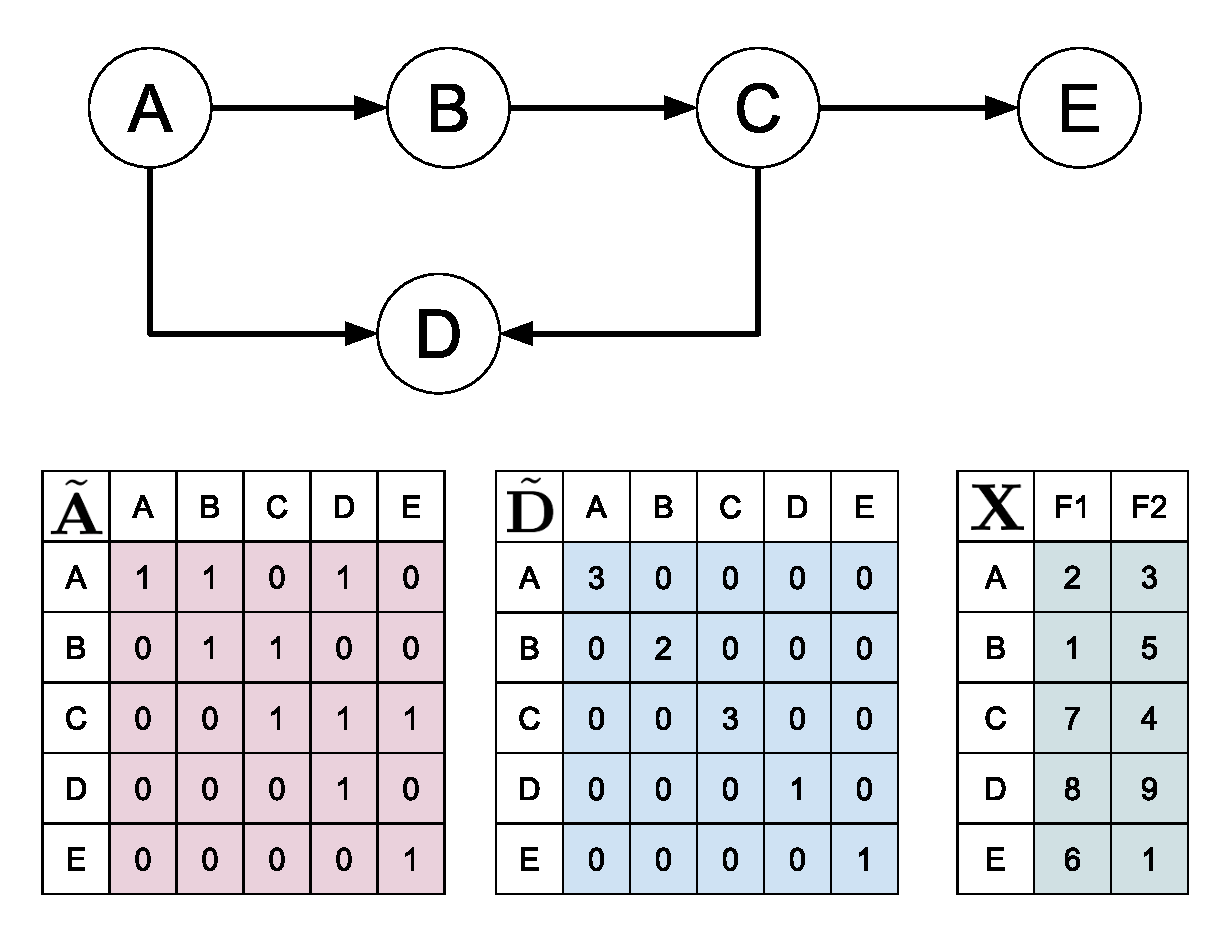
\includegraphics[width=0.90\textwidth]{Magic/figures/ExampleGraph.eps}}
\caption{An Example Graph $g$ and its Corresponding Matrices.}
\label{MG:Fig:ExampleGraph}
\end{figure*}

\textbf{Graph Convolution Layer(s).} In the first stage, a \textit{graph convolution} technique propagates each vertex's attributes to its neighborhood based on the structural connectivity.
To aggregate multi-scale sub-structural attributes, multiple graph
convolution layers are stacked, which can be defined recursively as follows:
\begin{equation}
    \mathbf{Z}^{t + 1} = f(\tilde{\mathbf{D}}^{-1} \tilde{\mathbf{A}} \mathbf{Z}^t \mathbf{W}^t)
\end{equation}
where $Z^0 = X$. The $t$-th layer takes input $Z^t \in \mathbb{Z}^{n \times c_t}$,
mapping $c_t$ feature channels into $c_{t+1}$ feature channels with the graph convolution parameter $\mathbf{W}^t \in \mathbb{R}^{c_t \times c_{t+1}}$.
The newly obtained channels of each vertex are then propagated to both its neighboring vertices and itself,
 first multiplied with the augmented adjacency matrix $\tilde{\mathbf{A}}$,
and then normalized row-wisely using the augmented degree diagonal matrix $\tilde{\mathbf{D}}$.
This key step enables vertices to pass its own attributes through the graph in a breadth-first-search fashion. %It can be explained as follows.
Define $\mathbf{F} = \mathbf{Z}^t \cdot \mathbf{W}^t$ and $\mathbf{O} = \tilde{\mathbf{A}} \cdot \mathbf{F}$, where
\begin{align}
    \mathbf{O}[i][j] &= \sum_{k = 1}^{n} \tilde{\mathbf{A}}[i][k] \times \mathbf{F}[k][j]
\end{align}
$\forall 1\leq i \leq n, 1 \leq j \leq c_t$.
In other words, the $j$-th feature channel of vertex $i$ is computed as a linear combination of all its neighbors' $j$-th feature channels.
The layer finally outputs the element-wise activation using a nonlinear function $f$.
At the end of $h$ graph convolution layers, DGCNN concatenates each layer's output $Z^{t}$,
denoted as $\mathbf{Z}^{1:h} = [\mathbf{Z}^1, \mathbf{Z}^2, \ldots, \mathbf{Z}^{h}]$.
For the sample graph $g$, Figure~\ref{MG:Fig:ExampleGraphConvolution} shows how the two sequential graph convolution layers transform the initial attribute matrix $\mathbf{Z}_0=\mathbf{X}$ to $\mathbf{Z}_1$ and $\mathbf{Z}_2$, both of which together form $\mathbf{Z}^{1:2}$.
After applying $h=2$ graph convolution layers, the sample graph $g$ is transformed to $\mathbf{Z}^{1:h}$.
We assume the weight parameters in the two graph convolution layers are $\mathbf{W}^1 = [[1, 0 ,1], [0, 1, 0]]$ and $\mathbf{W}^2 = [[0, 1 ,-2, 2], [1, 1, 7, -2], [1, 0, -1, 4]]$.
For simplicity, numbers are of 2 precision, and we perform the element-wise RELU nonlinear activation $f(x) = max(x, 0)$ in both graph convolution layers.

\begin{figure*}[htbp]
\centerline{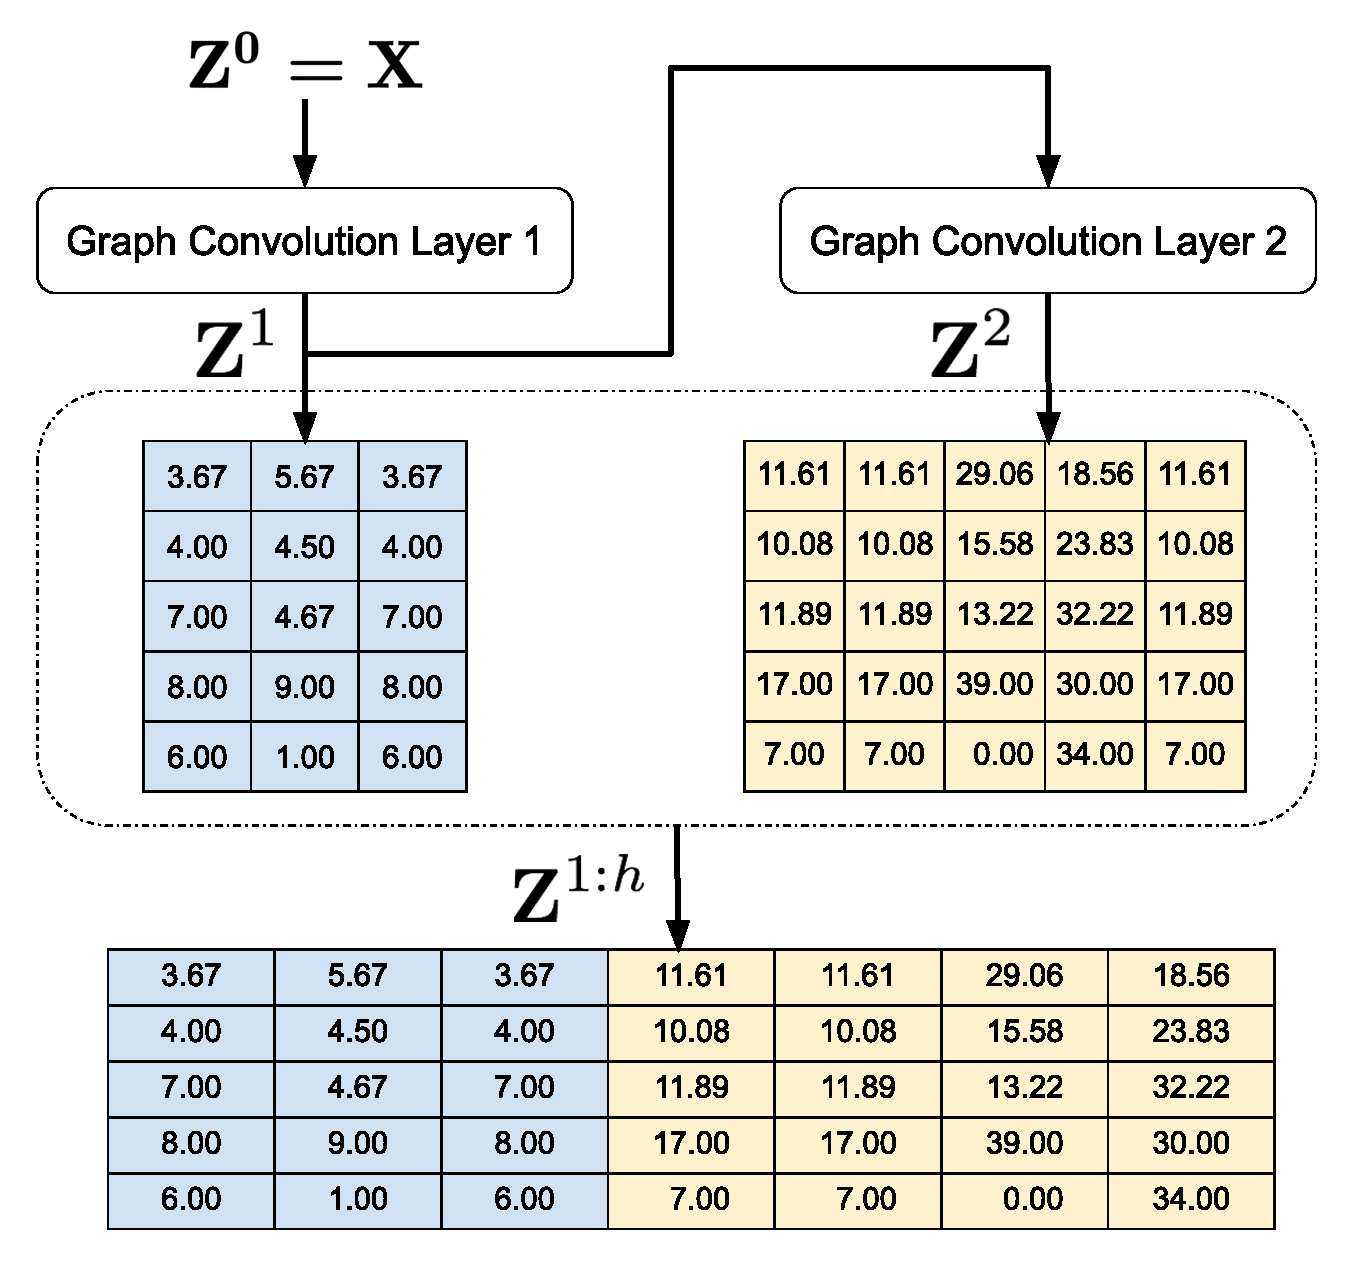
\includegraphics[width=0.90\textwidth]{Magic/figures/ExampleGraphConvolution.eps}}
\caption{Applying $h=2$ Graph Convolution Layers to Example Graph $g$}
\label{MG:Fig:ExampleGraphConvolution}
\end{figure*}

\textbf{SortPooling Layer.} Intuitively $\mathbf{Z}^{1:h}$ has $n$ rows and $\sum_{1}^{h}c_t$ column, which
corresponds to the \textit{feature descriptor} of each vertex at different scales.
The second stage, namely the \textit{sortpooling} layer,
leverages the feature descriptors to sort the vertices.
Vertices in different graphs will be put in similar positions as long as they have similar weighted feature descriptors.
The sortpooling layer starts with the last layer because $\mathbf{Z}^{h}$ is approximately
equivalent to the most refined continuous colors as in the Weisfeiler-Lehman graph kernels~\cite{WlGraphKernel}.
More specifically, vertices are first sorted by the last channel of the last layer in a decreasing order.
%When a tie on the last channel occurs, sorting will use the second last channel.
If there are $c_h$ ties on the last layer's output $\mathbf{Z}^{h}$,
sorting continues by using the second last layer's output $\mathbf{Z}^{h - 1}$, and the procedure repeats until all ties are broken.
The sortpooling layer further truncates or pads the sorted tensors by the first dimension so that it outputs $\mathbf{Z}^{sp}$ of size $k$ by $\sum_{1}^{h}c_t$.
Hence, the sortpooling process unifies the size of feature descriptors for all graphs.
Following our sample graph $g$, we visualize this process in Figure~\ref{MG:Fig:ExampleSortpool}.
Given the graph convolution result $\mathbf{Z}^{1:h}$ for the sample graph $g$ in Figure~\ref{MG:Fig:ExampleGraphConvolution},
the sortpooling layer with $k = 3$ sorts the feature descriptors (based on only the last feature channel in this example) and then truncates the two `smallest' rows.
The row of $\mathbf{Z}^{h}$ is first sorted using only the value in the last column.
The last two rows (i.e., yellow and red) are discarded from the sorted matrix as $n - k = 2 > 0$.

\textbf{Remaining Layer(s).} In the last stage, the authors of the original DGCNN\cite{Dgcnn} append a one-dimension convolution (Conv1D) layer of kernel size $\sum_{1}^{h}c_t$ and stride size $\sum_{1}^{h}c_t$.
If $F$ is the number of filters in the last one-dimension convolution layer, the sort pooling output $\mathbf{Z}^{sp}$ will be reduced to a one-dimension vector of size $k \times F$, which is then fed into a fully connected one-layer perceptron for graph classification.

\begin{figure*}[htbp]
\centerline{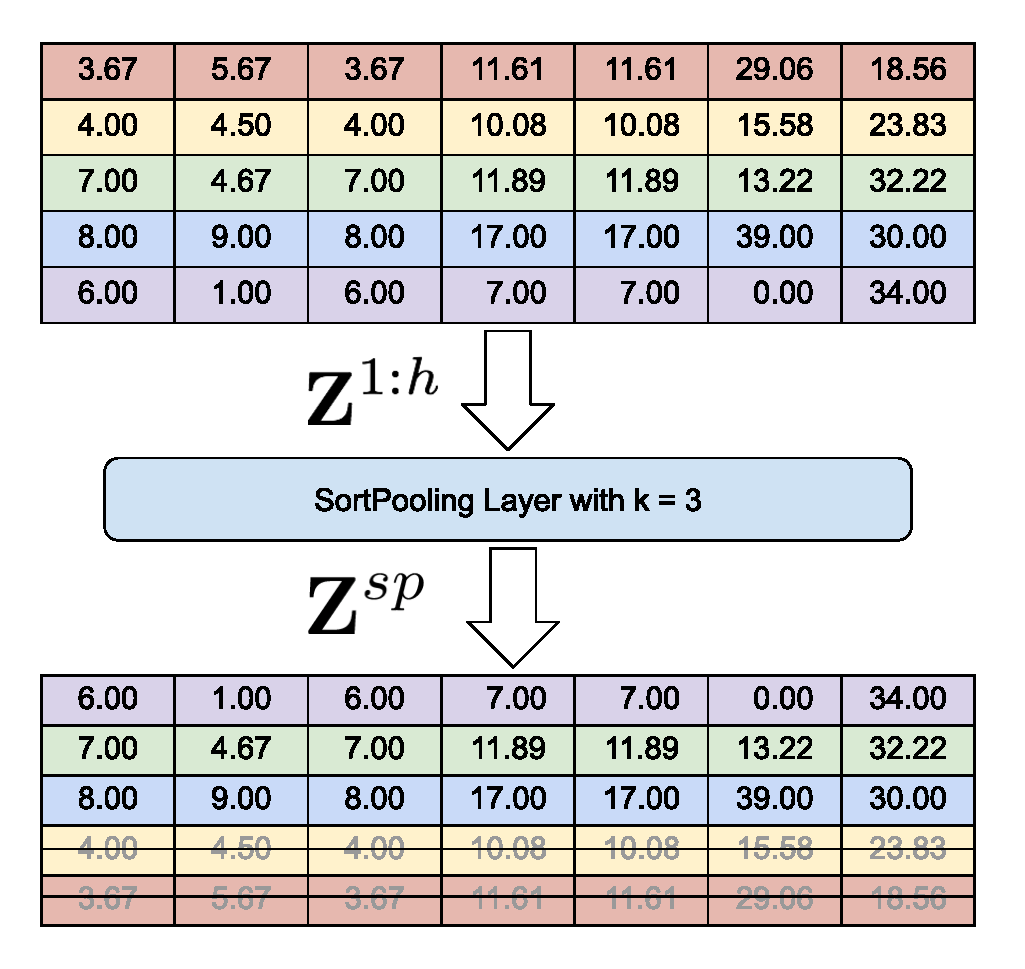
\includegraphics[width=0.90\textwidth]{Magic/figures/ExampleSortpool.eps}}
\caption{Applying Sortpooling Layer to Example Graph $g$}
\label{MG:Fig:ExampleSortpool}
\end{figure*}

\subsection{WeightedVertices Layer}
In the first extension to DGCNN, we observe that the Conv1D layer following the sortpooling layer can alternatively be of kernel size $k$, stride size $k$, and single channel.
Mathematically, a single channel Conv1D layer can be represented as a row of parameters $W \in \mathbb{R}^{1 \times k}$.
Its output $E \in \mathbb{R}^{1 \times \sum_{1}^{h}c_t}$, when fed with \textit{transposed} $\mathbf{Z}^{sp}$, will be equivalent to
\begin{equation}
    E = f(\mathbf{W} \times \mathbf{Z}^{sp})
\label{MG:Equ:WeightedVertices}
\end{equation}
%which is obviously after we notice that
This is because
\begin{equation}
    E_c = f(\sum_{i}^{k} W_i \times \mathbf{Z}^{sp}_{i, c})
\end{equation}
where $1\leq c \leq \sum_{1}^{h}c_t$, and $f$ is an element-wise nonlinear activation function.
Inspired by the graph embedding idea in\cite{GraphEmbedding}, our Conv1D layer treats each row of the sort pooling result $\mathbf{Z}^{sp}_{i}$ as the embedding of the vertices kept by the sortpooling layer.

Equivalently, Equation~(\ref{MG:Equ:WeightedVertices}) computes $E$, the embedding of the graph obtained through a weighted summation of vertex embeddings \cite{GraphEmbedding}.
For our sample graph $g$, its ``embedding" is computed in Figure~\ref{MG:Fig:ExampleWeightedVertice}, where we assume weight vector $\mathbf{W}=[0.4, 0.1, 0.5]$.
WeightVertices layer aggregates sample graph $g$'s vertex embeddings,
e.g. the output of sort pooling layer $\mathbf{Z}^{sp}$ in Figure~\ref{MG:Fig:ExampleSortpool}, to graph embedding $E$.
We choose again RELU as the nonlinear activition function $f$ for simplicity.
In reality, $\mathbf{W}$ is updated by gradient descent during the process of minimizing the classification loss.
For ease of presentation, in the remainder of the paper we refer to this special Conv1D layer after the sortpooling layer as the \textit{WeightedVertices} layer.
We replace the original Conv1D layer with the WeightVertices layer, because the WeightVertices layer leverages the graph embedding idea to make the output from the sorting pooling layer compatible with the malware classifier.

\begin{figure*}[htbp]
\centerline{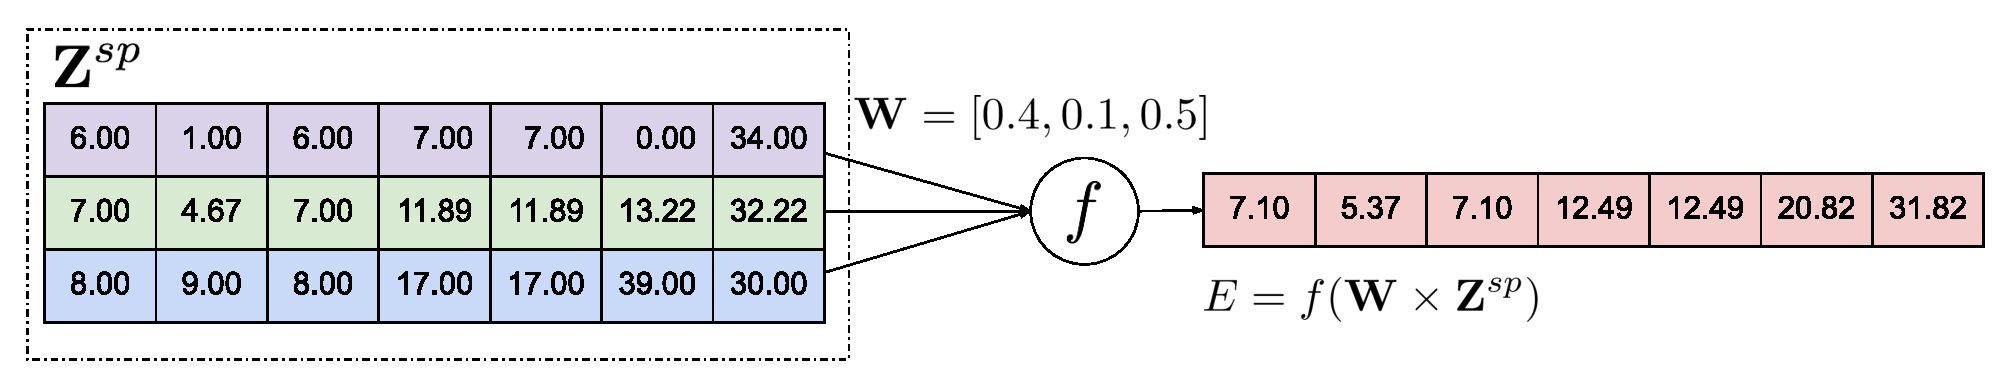
\includegraphics[width=0.90\textwidth]{Magic/figures/ExampleWeightedVertice.eps}}
\caption{Applying WeightVertices Layer to Example Graph $g$.}
\label{MG:Fig:ExampleWeightedVertice}
\end{figure*}

\subsection{AdaptiveMaxPooling: An Alternative to Sortpooling}
The intuition behind sorting from the deeper layer is to treat its output as more refined WL colors\cite{WlAlgorithm, WlGraphKernel}.
The inner sorting inside the channels of a fixed layer output is, however, less reasonable.
Besides, the Conv1D addendum is only aggregating the feature descriptors of per vertex and per convolution channel separately.

Our second extension is to apply the adaptive max pooling (AMP) on the concatenated graph convolution layer output $\mathbf{Z}^{1:h}$.
Given an set of two-dimension inputs of various sizes $\{x_i | x_i \in \mathbb{R}^{h_i \times w_i}\}$,
The AMP layer divides each input $x_i$ into a $H \times W$ grid with a sub-window size approximately to $h_i / H$ and $w_i / W$,
and then automatically chooses kernel sizes as well as convolution strides for different $x_i$.
Inside each sub-window and each channel, only the maximum element is kept in order to form the set of identical-dimension outputs $\{y_i | y_i \in \mathbb{R}^{ H \times W}\}$.
The way in which AMP works for our sample graph $g$ is illustrated in Figure~\ref{MG:Fig:ExampleAmp}.
The left top matrix $\mathbf{Z}^{1:h}_g$ represents the graph convolution output of the sample graph $g$ in Figure~\ref{MG:Fig:ExampleGraph}.
The left bottom matrix $\mathbf{Z}^{1:h}_{g'}$ represents the graph convolution output of another imaginary graph $g'$ with four vertices.
For $\mathbf{Z}^{1:h}_g$ of size $5\times 7$, adaptive max pooling's kernel size = $3 \times 3$ (shown as red shadow).
For $\mathbf{Z}^{1:h}_{g'}$ of size $4\times 7$, adaptive max pooling's kernel size = $2 \times 3$ (shown as red shadow).
For both inputs, padding = 0, stride = $2 \times 1$.
Since the dimension of the graph convolution output $\mathbf{Z}^{1:h}_g$ for $g$ is $5 \times 7$, AMP uses a max pooling kernel of size $3 \times 3$.
To show how AMP works for inputs of different dimension sizes, in Figure~\ref{MG:Fig:ExampleAmp} we also feed $\mathbf{Z}^{1:h}_{g'}$,
the graph convolution output for another graph $g'$ (not shown here), to the $3 \times 3$ AMP layer.
In this case, the kernel size is adaptively adjusted to $2 \times 3$.

We have two motivations for using AMP at the end of the graph convolution layer.
In addition to unifying the convolution layer output $\mathbf{Z}^{1:h}$, AMP empowers us to aggregate $\mathbf{Z}^{1:h}$
across the dimensions of both feature channels and graph vertices simultaneously,
which enables us to capture informative features that vary only by location.
This is easily accomplished by applying a two-dimension convolution (Conv2D) layer with an arbitrary number of filters before the AMP layer.
The output of the AMP layer is further fed into a multiple-Conv2D-layer neural network, inspired by VGG~\cite{VGG}, to predict the probability distribution of the malware families that the input CFG should belong to.

\begin{figure*}[htbp]
\centerline{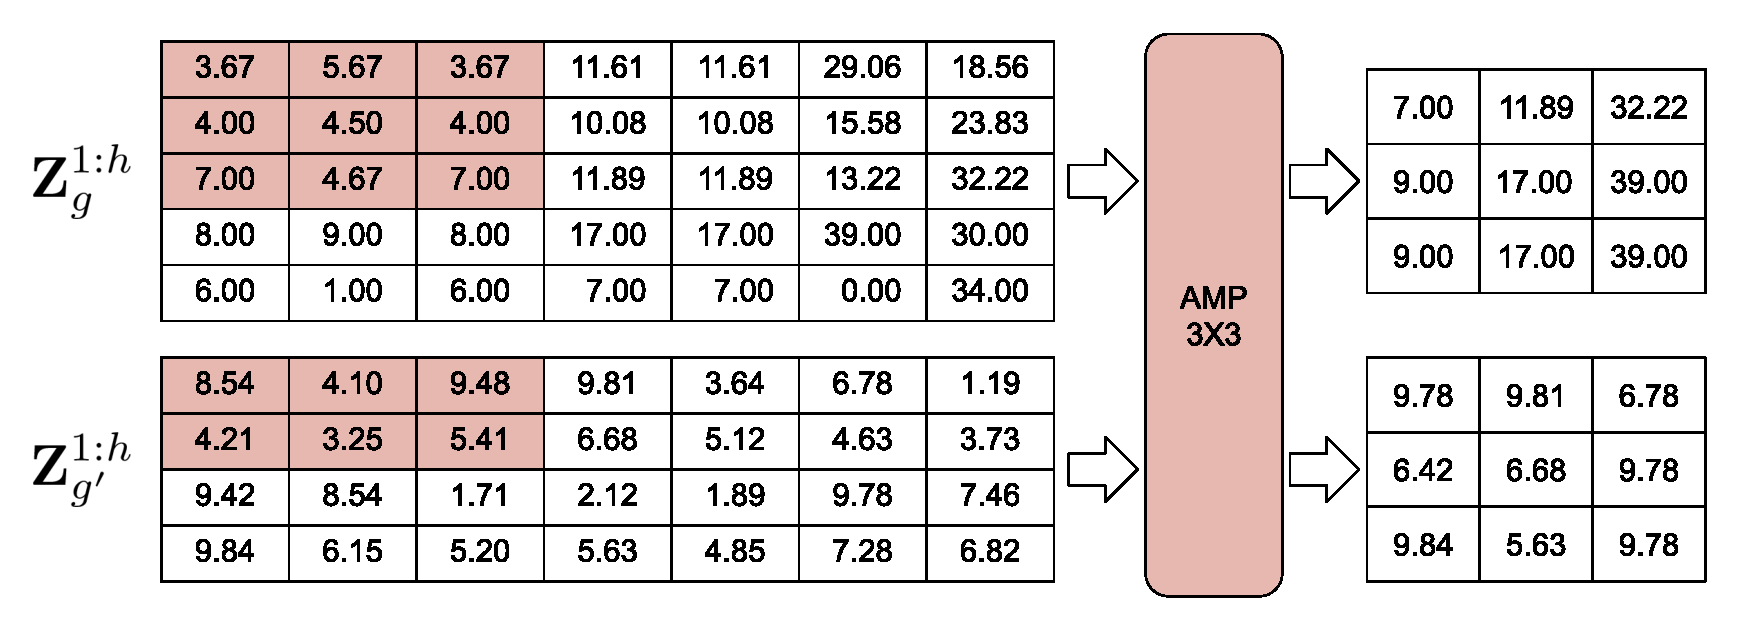
\includegraphics[width=0.90\textwidth]{Magic/figures/ExampleAmp.eps}}
\caption{Applying AdaptiveMaxPooling Layers to Example Graph $g$.}
\label{MG:Fig:ExampleAmp}
\end{figure*}

\section{Implementation}
\label{MG:Sec:Implement}

In this section, we discuss a few implementation details, which include how we derive CFGs from dissembled code, what kind of loss functions are used in model training, and the open source MAGIC project.

\subsection{Details in Building CFG}
\label{MG:SubSec:BuildCfg}
To build a control flow graph from disassembled code in possibly different formats, we first pre-process the input files so that the resulting program $P$ is a one-to-one mapping from \textit{sorted addresses} to \textit{assembly instructions}, e.g., $P: \mathbf{Z}^+ \rightarrow \mathbf{I}$.

We then perform a two-pass iteration over $P$.
Instructions $inst \in \mathbf{I}$ are associated with a couple of tags,
i.e., \texttt{\{start, branchTo, fallThrough, return\}}, used by the second pass for creating code blocks and connecting blocks.
To adapt to (potentially) hundreds of types of instructions, the first pass applies the visitor pattern to implement if-else free instruction tagging.
As an example, Algorithm~\ref{MG:Alg:CallExample} details the tagging operations when visiting a conditional jump instruction $cj$.
This procedure relies on a helper function \texttt{findDstAddr($inst$)} to extract the destination address of a jump instruction $inst$.
For a conditional jump instruction,
it branches to the jump target ($P[dstAddr]$, handled by line 2 -- 3) and falls through to the next instruction ($P[cj.addr + cj.size]$, handled by line 4 -- 5).

%\begin{algorithm}
%\caption{\texttt{visitConditionalJump($cj$)}}
%\label{MG:Alg:CallExample}
%\begin{algorithmic}[1]
%\STATE $dstAddr \leftarrow \texttt{findDstAddr}(cj)$
%\STATE $cj.branchTo \leftarrow dstAddr$
%\STATE $P[dstAddr].start \leftarrow true$
%\STATE $cj.fallThrough \leftarrow true$
%\STATE $P[cj.addr + cj.size].start \leftarrow true$
%\end{algorithmic}
%\end{algorithm}

\begin{algorithm}[t]
    \DontPrintSemicolon
    \KwData{$cj = $ a conditional jump instruction \newline
            $P = $ program, e.g., mapping from instruction address to instruction}
    $dstAddr \gets \texttt{findDstAddr}(cj)$\;
    $cj.branchTo \gets dstAddr$\;
    $P[dstAddr].start \gets true$\;
    $cj.fallThrough \gets true$\;
    $P[cj.addr + cj.size].start \gets true$\;
    \caption{\texttt{visitConditionalJump($cj$)}}
    \label{MG:Alg:CallExample}
\end{algorithm}

The second pass creates code blocks (or vertices) and connects blocks on the fly.
The skeleton of the procedure is illustrated in Algorithm~\ref{MG:Alg:SecondPass}.
Algorithm~\ref{MG:Alg:SecondPass} assumes two trivial helper functions.
Firstly, \texttt{getBlockAtAddr($addr$)} returns the block starting at $addr$
if it already exists; otherwise it creates a new block starting at $addr$.
The second one \texttt{getNextInst($P, inst$)} returns the instruction next to $inst$ if it exists; otherwise, \texttt{None} is returned.
With both helpers, Algorithm~\ref{MG:Alg:SecondPass} works in three steps.
The first if statement creates a new block if $inst$ was marked as \texttt{start} in the first pass.
The second step connects $block$ to $nextBlock$ if the last instruction in $block$ is falling through to the next instruction, which happens to be the start of $nextBlock$.
The final step creates an edge (potentially a new block) for any branching operations, e.g., jump or call.

%\begin{algorithm}
%\caption{\texttt{CfgBuilder::connectBlocks()}}
%\label{MG:Alg:SecondPass}
%\begin{algorithmic}[1]
%\FORALL{$inst$ in program $P$}
    %\IF{$inst.start$}
        %\STATE $currBlock \leftarrow \texttt{getBlockAtAddr}(inst.addr)$
    %\ENDIF
    %\STATE $nextBlock \leftarrow currBlock$
    %\STATE
    %\STATE $nextInst \leftarrow \texttt{getNextInst}(P, inst)$
    %\IF{$nextInst \neq$ None}
        %\IF {$inst.fallThrough$ \AND $nextInst.start$}
            %\STATE $nextBlock \leftarrow \texttt{getBlockAtAddr}(nextInst.addr)$
            %\STATE add $nextBlock$ to $currBlock$'s edge list
        %\ENDIF
    %\ENDIF
    %\STATE
    %\IF{$inst.branchTo \neq$ None}
        %\STATE $block \leftarrow \texttt{getBlockAtAddr}(inst.branchTo)$
        %\STATE add $block$ to $currBlock$'s edge list
    %\ENDIF
    %\STATE
    %\STATE add $inst$ to $currBlock$
    %\STATE $currBlock \leftarrow nextBlock$
%\ENDFOR
%\end{algorithmic}
%\end{algorithm}

\begin{algorithm}[t]
    \DontPrintSemicolon
    \KwData{$P = $ program, e.g., mapping from instruction address to instruction}
    \ForEach {$inst$ in program $P$} {
        \If{$inst.start$} {
            $currBlock \gets \texttt{getBlockAtAddr}(inst.addr)$\;
        }
        $nextBlock \gets currBlock$\;
        $nextInst \gets \texttt{getNextInst}(P, inst)$\;
        \If{$nextInst \neq$ None} {
            \If{$inst.fallThrough \land nextInst.start$} {
                $nextBlock \gets \texttt{getBlockAtAddr(nextInst.addr)}$\l\;
                add $nextBlock$ to $currBlock$'s edge list\;
            }
        }
        \If {$inst.branchTo \neq$ None} {
            $block \gets \texttt{getBlockAtAddr}(inst.branchTo)$\;
            add $block$ to $currBlock$'s edge list\;
        }
        add $inst$ to $currBlock$\;
        $currBlock \gets nextBlock$\;
    }
    \caption{\texttt{CfgBuilder::connectBlocks()}}
    \label{MG:Alg:SecondPass}
\end{algorithm}

\subsection{Loss Functions Used in Model Training}
Another technical advantage of \sysname is its support for the end-to-end deep neural network training.
Regardless of how we change the layer configurations, i.e., whether to use the sort pooling layer or the adaptive max pooling layer, the model's output is always the prediction of the observed input.
Therefore, the training procedure always minimizes the mean negative logarithmic loss, which is defined as
\begin{equation}
    \mathcal{L} = \sum_{i=1}^{N} \sum_{c=1}^{C} y_{i, c} \log(p_{i, c})
\end{equation}
where $N$ is the number of observations in the dataset, $C$ is the number of malware families in the dataset, 
$y_{i, c}$ is 1 if the $i$th sample belongs to malware family $c$,
and $p_{i, c}$ is the predicted probability that $i$th sample is in family $c$ in the output of the model.
We adopt the Adam optimization algorithm \cite{Adam} implemented in PyTorch \cite{PyTorch} to auto-generate the gradient of the model parameters and update the parameters in the DGCNN (e.g. $W^t, 1 \leq t \leq h$ in graph convolution layers) accordingly.

\subsection{Open Source \sysname Project}
%Depending on the DGCNN-based classifier, 
For malware classification tasks, \sysname runs either in the training mode or in the prediction mode.
In the training stage, we repeatedly activate only the first half of the pipeline to obtain a large amount of labeled CFGs.
Then, a DGCNN and its classifier are trained using the stochastic gradient descent on the labeled CFGs in a batch mode.
When the training finishes, \sysname takes the CFGs of unknown binary executables as inputs and make predictions.

We have implemented a prototype system of \sysname with approximately 4,000 line of Python code.
The implementation can be divided into two independent parts.
The first part generates ACFGs from either assembly code or control flow graphs.
Due to the necessity of processing a large number of assembly programs, \sysname can generate multiple ACFGs in parallel using Python's multi-threading library.
The second part handles the training, tuning, and evaluation of the extended DGCNN, which is built upon, but heavily rewritten, from Muhang's PyTorch implementation \cite{MuhanDgcnn}.
For example, we developed the adaptive pooling layer and the WeightedVertices layer.
Besides, MAGIC supports automatic and exhaustive hyper-parameter tuning, cross-validation, training and prediction using GPUs.
We will make \sysname's codebase publicly available at Github in the near future.

\section{Experimental Evaluation}
\label{MG:Sec:Experiment}

We evaluate the performance of \sysname using two large malware datasets, each with more than 10,000 samples, and present our experimental results in this section.

\subsection{Malware Datasets}
The first dataset, which we refer to as the \textit{MSKCFG} dataset, includes the CFGs derived from the malware files used in the 2015 Microsoft Malware Classification Challenge hosted by Kaggle~\cite{MsAcfgDataset}. The dataset contains samples that fall into nine families: \{Ramnit, Lollipop, Kelihos\_ver3, Vundo, Simda, Tracur, Kelihos\_ver1, Obfuscator.ACY, Gatak\}.
Figure~\ref{MG:Fig:MSKCFGLabelDist} presents the number of samples in each of these nine malware families in the dataset.
%The identification of benign code is not in the scope of the contest, and all the input files are supposed to be malicious.
In the competition, Kaggle provided 10,868 labeled malware samples as the training dataset, for each of which two files were given.
% Kaggle used another 10,873 malware samples, whose labels remained unknown to participants, to rank the submissions.
% We ignored 10 `empty'\footnote{A file is \textit{empty} if it contains only character `??', which means the data provider erased these byte information for certain reasons.} .byte files in training set and 13 empty ones in testing set respectively.
%Two files were given for each malware is represented as two files in the dataset.
The first file contains the raw binary content in a hexadecimal representation (referred as .byte file in the following discussion).
The second file is the corresponding assembly code of the binary code, which was generated with the IDA Pro tool~\cite{bib:idapro} (referred as .asm file in the following discussion).
The correctness of the .asm file is not guaranteed because PE headers were erased from the raw malware files for sterility before they were disassembled and sophisticated binary packing techniques may also prevent reverse engineering tools from disassembling the malware correctly~\cite{BinaryUnpacking}. 
In our experiments, only the .asm files were used for malware classification.
We generated a total number of 10,868 ACFGs from the training .asm files, which took approximately 17 hours to finish, or averagely 5.8 seconds per malware instance,
using a commodity desktop equipped with Intel Core i7-6850K CPU and 64 GB memory.
%These ACFGs are denoted as the \textit{MSKCFG} dataset hereafter.

Another dataset, which we refer to as \textit{YANCFG}, includes the CFGs of 16,351 binary executable files which were used in \cite{YanDataset}.
%The original dataset contains hexadecimal bytes from the original binary file and the features from both dynamic execution traces and PE headers.
%However, the dataset given to us are CFG format files.
Similar to the MSKCFG dataset, the PE headers were not available to us for malware classification from the second dataset. All the CFGs were labeled with a majority voting scheme based on the detection results of five major AV scanners returned by the VirusTotal online malware analysis service~\cite{VirusTotal}.
All the CFGs belong to 12 distinct malware families: \{Bagle, Benign, Bifrose, Hupigon, Koobface, Ldpinch, Lmir, Rbot, Sdbot, Swizzor, Vundo, Zbot, Zlob\}.
Figure~\ref{MG:Fig:YANCFGLabelDist} depicts the number of samples for each of these 12 families in the dataset.
These CFGs were further converted to their corresponding ACFGs by MAGIC within 6.8 hours using the same desktop machine as mentioned above.
%After the 6.8-hour CFG-to-ACFG conversion, we obtained 16,351 ACFGs.% further discarded 1,976 empty graphs.
%These ACFGs are stored together and referred as \textit{YANCFG} as a whole dataset.
%For clarity, we refer the second dataset as \textit{YANCFG}.
%We plan to make the resultant ACFGs on both public and private datasets available to the research community alongside with the system implementation of \sysname.


We did not merge two malware datasets in our experiments due to the following reasons.
Firstly, the YANCFG dataset carries pre-processed CFGs,
while we developed our own parser to extract CFGs from the malware assembly code in the Microsoft dataset (see Section~\ref{MG:SubSec:BuildCfg}).
% The differences in the methods used to extract CFGs from the two datasets may lead to inconsistent CFG representations for model training.
The CFG extracted from the MSKCFG dataset by our own parser has different low-level feature representation from that of the CFGs pre-given in YANCFG;
so they cannot be applied to one model.
Secondly, testing MAGIC on datasets collected from independent sources also allows us to gain insights into its generality when applied in different operational environments.

\begin{table*}[htbp]
\caption{Hyperparameters and Search Ranges during Tuning}
\begin{center}
\begin{tabular}{l|r|r|r}
\hline
Hyperparameter & Choice or Value Range & Best Model for MSKCFG & Best Model for YANCFG \\
\hline
\hline
Pooling Type & [Adaptive Pooling, Sort Pooling] & Adaptive Pooling &  Adaptive Pooling\\
\hline
Pooling Ratio & [0.2, 0.64] & 0.64 & 0.2 \\
\hline
Graph Convolution Size & [(32, 32, 32, 1)\tablefootnote{Only for sort pooling}, (32, 32, 32, 32), (128, 64, 32, 32)] & (128, 64, 32, 32) & (32, 32, 32, 32)\\
\hline
Remaining Layer\tablefootnote{Applicable only when set \textit{pooling type} to sort} & [1D Convolution Layer, WeightVertices Layer] & Not Applicable &  Not Applicable \\
\hline
2D Convolution Channels\tablefootnote{Applicable only when set \textit{pooling type} to adaptive pooling} & [16, 32]  & 16 & 16 \\
\hline
1D Convolution Channel Pairs\tablefootnote{Applicable only when set \textit{pooling type} to sort pooling and \textit{remaining layer} to 1D convolution} & [(16, 32)] & Not Applicable & Not Applicable \\
\hline
1D Convolution Kernel Size\tablefootnote{Applicable only when set \textit{pooling type} to sort pooling and \textit{remaining layer} to 1D convolution} & [5, 7] & Not Applicable & Not Applicable\\
\hline
Dropout Rate & [0.1, 0.5] & 0.1 & 0.5 \\
\hline
Batch Size & [10, 40] & 10 & 40\\
\hline
Weight L2 Regularization Factor & [0.0001, 0.0005] & 0.0001 & 0.0005\\
\hline
\end{tabular}
\label{MG:Tab:Hyperparameters}
\end{center}
\end{table*}

\subsection{Model Training and Evaluation}
As the malware families are different in the two datasets, we need to create two different \sysname instances to classify their malware samples separately. However, MAGIC uses the same way to train DGCNN and tune its hyperparameters for both datasets.
The first step is hyperparameter tuning.
Table~\ref{MG:Tab:Hyperparameters} lists the hyperparameters used in both the deep neural network itself (e.g., the sizes of the graph convolution layers) and the algorithm for training the model (e.g., batch size and learning rate).
To determine the optimal values of these hyperparameters,
we exhaustively search all 208 hyperparameter settings defined by the value ranges listed in Table~\ref{MG:Tab:Hyperparameters}.
In particular, 64 DGCNN models use adaptive pooling, 96 DGCNN models use the sort pooling and Conv1D layer, and 48 DGCNN models use the sort pooling and WeightVertices layer.
We apply the five-fold cross-validation technique to evaluate the performance of a model under a specific hyperparameter setting.
To conduct five-fold cross validation, the dataset is splitted into five equal-size subsets.
In each fold of the cross validation, four subsets (80\%) of the data are used for training a brand new model initialized randomly,
and the rest subset (20\% of the data), different in each fold, is used to evaluate the resultant model.
In this way, the training process never sees the testing samples used for performance evaluation.
We train each model with 100 epochs and record the negative log-likelihood validation loss after every epoch.
%The average loss score over the five cross-validation runs is reported.

The validation loss collected after each epoch is used to find the hyperparameters that can mitigate the overfitting issue. Once the validation loss increases for two continuous epochs,
we decrease the learning rate by a factor of ten to prevent the model from overfitting the training dataset.
For a particular model, when all five training-validation folds are finished, we compute each epoch's validation loss by averaging the five validation losses over the five folds.
The minimum validation loss over the 100 epochs is treated as the score of this model and is further used as the criterion for comparing with different hyperparameter settings.
In other words, after the five-fold cross-validation for all the 208 model training instances, we choose the best model with the minimum average validation loss.
%To compare our best model's performance to previous works, 
Besides the average validation negative log-likelihood loss,
we also measure its precision, recall, and F1 score averaged over the five validation sets (together referred to as the \emph{cross-validation scores}), and then compare the best model's performance against those of previous works.
We used four GeForce GTX 1080 Ti graphic cards to train and run the 208 variants of DGCNN.
Training a particular model is always done on a single GPU,
but the evaluation procedure actually takes up all the four GPUs because our \sysname implementation supports parallel model training on multiple GPUs.
The last two columns in Table~\ref{MG:Tab:Hyperparameters} describe the best models chosen by MAGIC for the MSKCFG and YANCFG datasets, respectively.
% Confusion matrix for a random validation set is also included.
%Their cross-validation scores are reported in the following two sub-sections for both MSKCFG and YANCFG dataset respectively.
In the following, we report the cross-validation scores for the two datasets.

\begin{figure}
\centerline{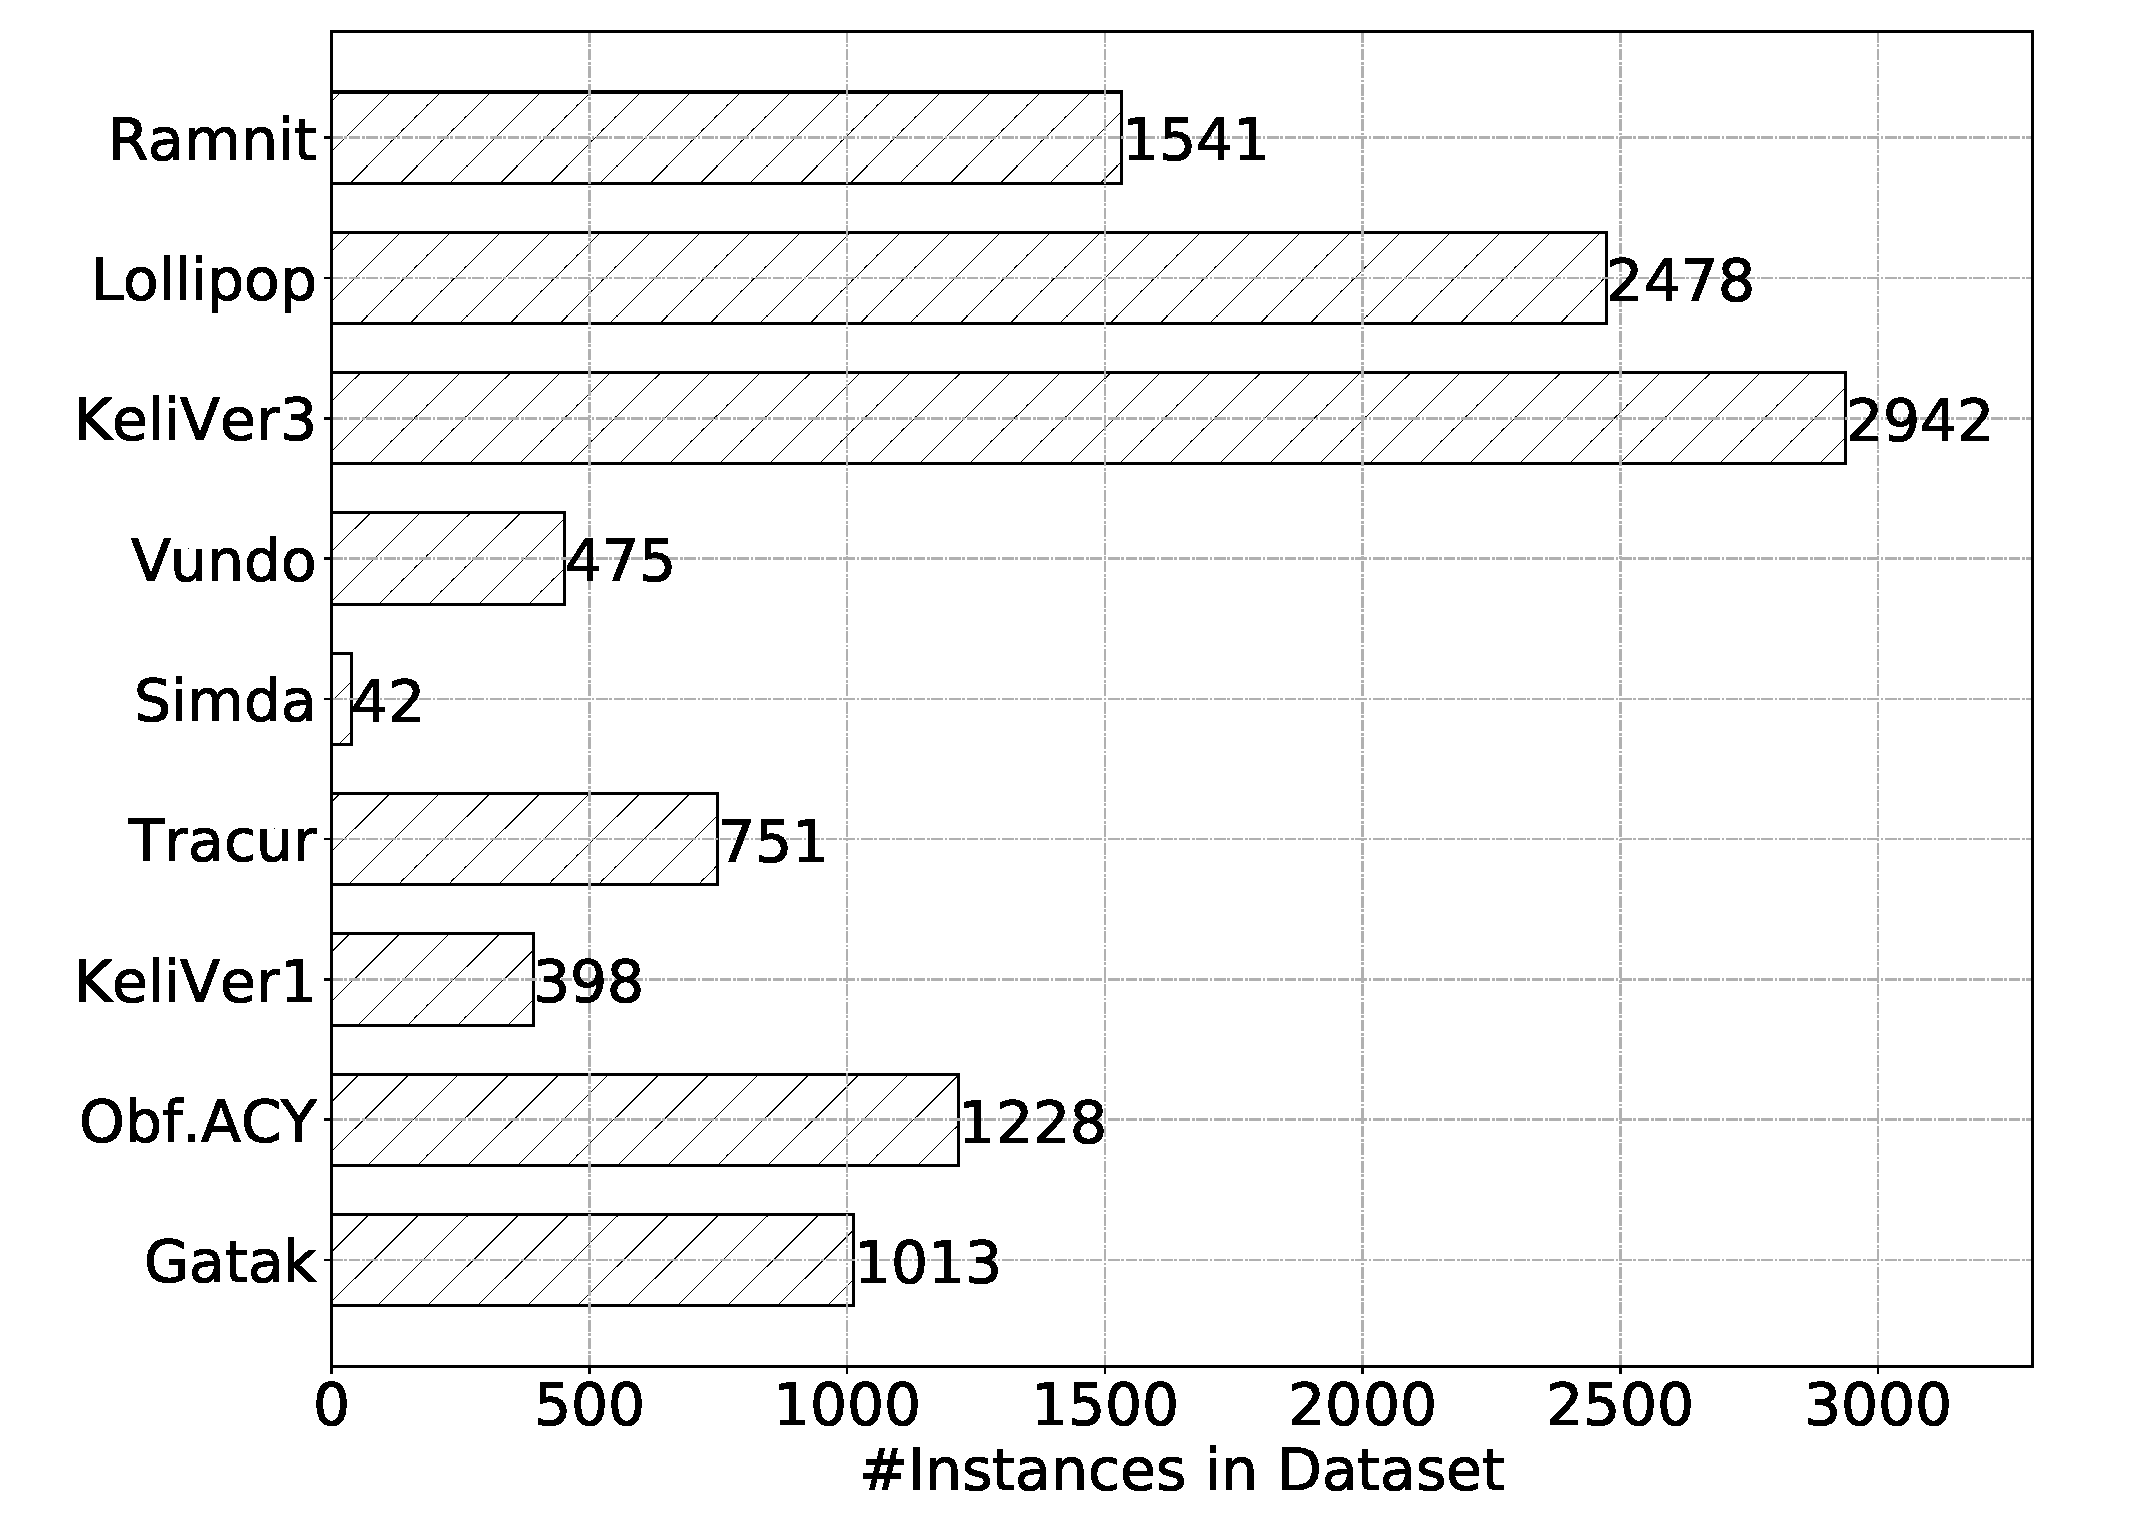
\includegraphics[width=0.44\textwidth]{Magic/figures/MsAcfgLabelDist.eps}}
\caption{Malware Family Distribution in MSKCFG Dataset.}
\label{MG:Fig:MSKCFGLabelDist}
\end{figure}

\begin{figure}
\centerline{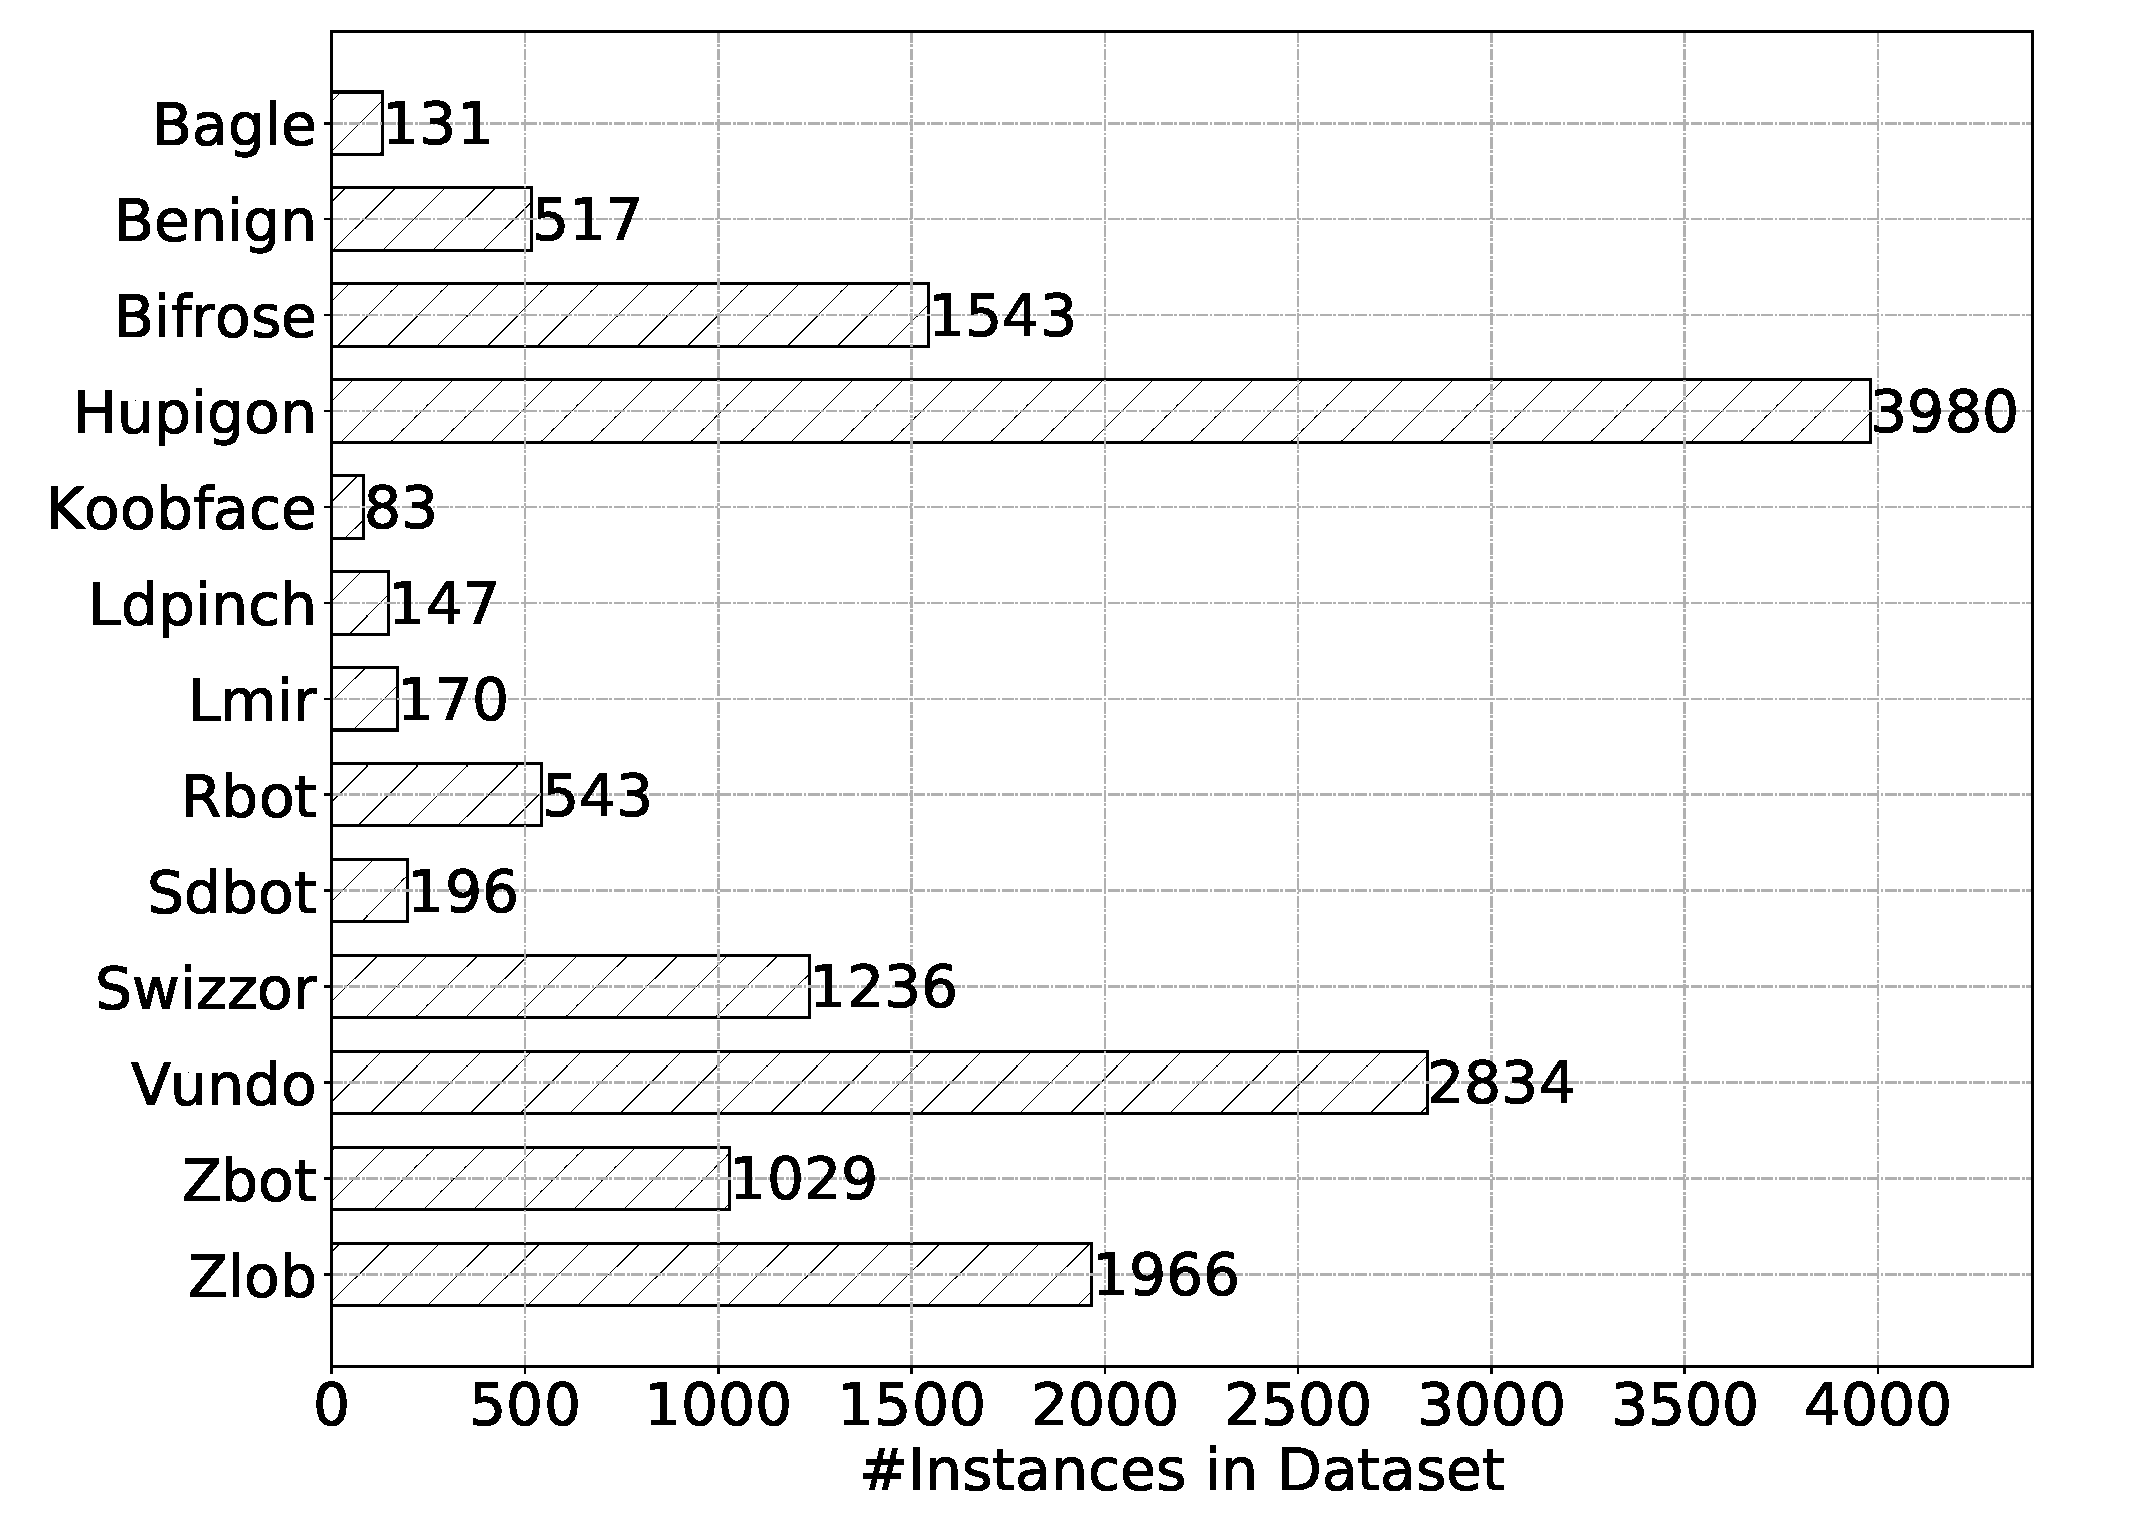
\includegraphics[width=0.44\textwidth]{Magic/figures/YanAcfgLabelDist.eps}}
\caption{Malware Family Distribution in YANCFG Dataset.}
\label{MG:Fig:YANCFGLabelDist}
\end{figure}

\subsection{Results on the MSKCFG Dataset}
The best cross-validation scores (precision, recall and F1) for the MSKCFG dataset are shown in Figure~\ref{MG:Fig:MSKCFGScores}, and the exact score values are listed in Table~\ref{MG:Tab:MSKCFGScores}.
The standard variances are not listed because the scores' variations among five different cross-validation folds are negligible ($<0.004$).
% Table~\ref{tab:MSKCFGConfusionMatrix} details the corresponding confusion table.
For all nine malware families, our best model has achieved good validation scores with precisions higher than 0.96, recalls higher than 0.96, and F1-scores higher than 0.97.

\begin{figure}
\centerline{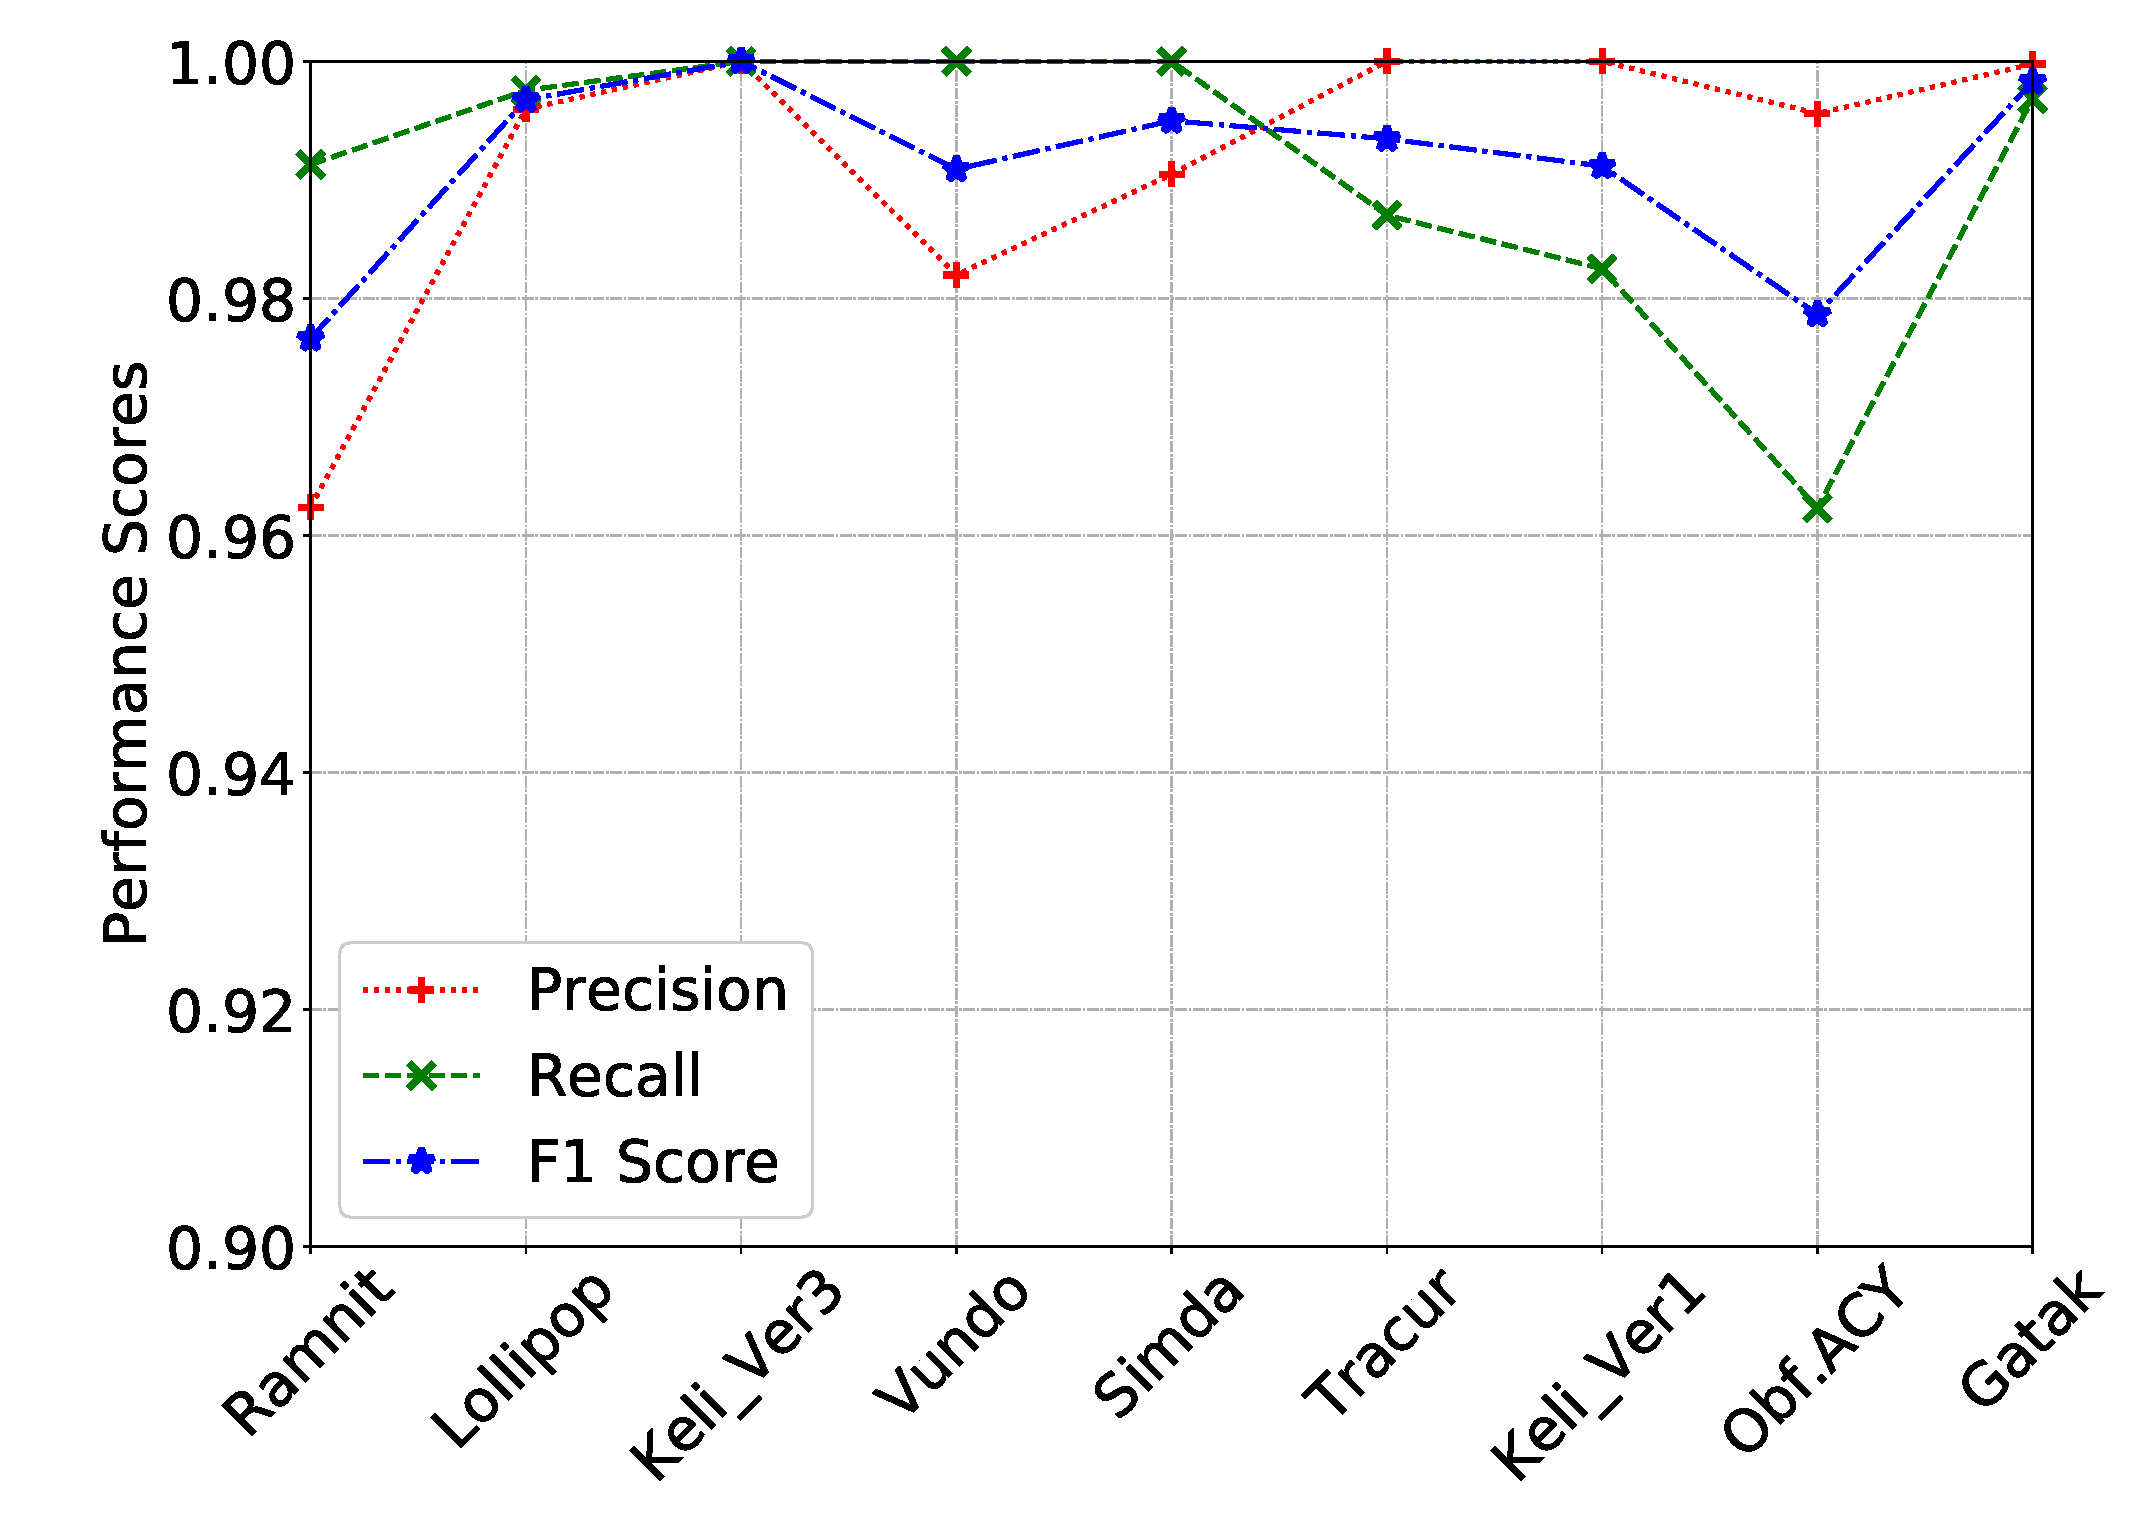
\includegraphics[width=0.44\textwidth]{Magic/figures/MsAcfgScores.eps}}
\caption{Cross-Validation Scores of \sysname on the MSKCFG Dataset.}
\label{MG:Fig:MSKCFGScores}
\end{figure}

\begin{table}
\caption{Performances of \sysname on the MSKCFG Dataset.}
\begin{center}
\begin{tabular}{l|rrr}
\hline
   Family       &  Precision &    Recall &        F1 \\
\hline
\hline
   Ramnit       &   0.962378 &  0.991289 &  0.976615 \\
 Lollipop       &   0.995960 &  0.997550 &  0.996754 \\
 Kelihos\_Ver3  &   1.000000 &  1.000000 &  1.000000 \\
    Vundo       &   0.981975 &  1.000000 &  0.990895 \\
    Simda       &   0.990476 &  1.000000 &  0.994987 \\
   Tracur       &   1.000000 &  0.987013 &  0.993463 \\
 Kelihos\_Ver1  &   1.000000 &  0.982493 &  0.991156 \\
Obfuscator.ACY  &   0.995593 &  0.962293 &  0.978655 \\
    Gatak       &   0.999775 &  0.996841 &  0.998304 \\
\hline
\end{tabular}
\end{center}
\label{MG:Tab:MSKCFGScores}
\end{table}

Since Microsoft released the competition dataset in 2015, many researchers have used the dataset (completely or partially) to evaluate their techniques for malware detection and classification~\cite{NovelFeatureFusion, EnsembleDNN, AutoEncoderMicrosoft, FunctionCallGraph, StaticFeatures, PolySeqCls, AutoEncoderFeatureLearn, YuxinMalwareDnn}.
We surveyed the works mentioned above and found that three of them cannot be directly compared with our results because they were using different metrics.
%and found that unfortunately every work either performed the evaluation in a unique way or gave their evaluation results using divided metrics due to varying reasons, making three works not directly comparable to ours. 
The works in \cite{EnsembleDNN} and \cite{YuxinMalwareDnn} used the Microsoft dataset in the context of \emph{malware detection}, where all the samples contained within it were treated as malicious, and then they were merged with a number of benign programs to construct a new dataset for malware detection.
As a result, their methods and performance metrics (two-class AUC, F1 score or accuracy) are not directly comparable to the approaches aimed at classifying malware samples into the corresponding families (e.g.,~\cite{NovelFeatureFusion, AutoEncoderMicrosoft, FunctionCallGraph, StaticFeatures, PolySeqCls, AutoEncoderFeatureLearn}), this work included. %, where models should predict the malware family that a sample belongs to.
Note that without loss of generality, benign software can be treated as a special family.
The work in~\cite{AutoEncoderMicrosoft} did not adopt the cross-validation methodology. Instead, the authors manually split the training dataset into 75\% training data and 25\% holdout testing data, and reported the mean square error, accuracy and confusion matrix over both training and testing data.
The holdout set is not the test set provided by Microsoft. 
Therefore, we did not compare our work with the evaluation results reported in \cite{EnsembleDNN}, \cite{YuxinMalwareDnn} and \cite{AutoEncoderMicrosoft}.

Among the other five papers of malware classification, both \cite{FunctionCallGraph} and \cite{StaticFeatures} conducted the ten-fold cross validation over the Microsoft dataset, but only reported the overall accuracy.
\cite{PolySeqCls} also performed a ten-fold cross validation but reported both the overall accuracy and logarithmic loss.
Both \cite{NovelFeatureFusion} and \cite{AutoEncoderFeatureLearn} performed a five-fold cross validation and reported both the overall accuracy and logarithmic loss.
Since the Microsoft dataset is not balanced across malware families, we compare \sysname with the five previous works that reported not only the overall accuracy but also the mean logarithmic loss, and the results are shown in Table~\ref{MG:Tab:CompareMicrosoftCv}.

The methods listed in Table~\ref{MG:Tab:CompareMicrosoftCv} can be classified into either ensemble-learning or single-model based approaches.
\cite{NovelFeatureFusion} extracts more than 1800 features and uses gradient boosting based classifier, and it achieves the best log-loss (0.0197) and accuracy (99.42\%) using the XGBoost classifier. 
\cite{FunctionCallGraph} achieves the second best accuracy (99.3\%) by ensembling multiple random forest methods, which already ensembles multiple decision trees.
The DGCNN-based technique used by MAGIC achieves highly competitive results.
In fact, the logarithmic loss (0.0543) is the second best; the accuracy (99.25\%) is the third best, only 0.005 less than the second best one (99.3\% reported by \cite{FunctionCallGraph}).
\cite{AutoEncoderFeatureLearn} adopts a deep-learning based hybrid approach.
It relies on a single deep autoencoder to perform automatic feature learning, and then uses gradient-boosting based classifier to make the prediction.
As an alternative work that also applies deep neural network, our DGCNN-based approach outperforms the work in~\cite{AutoEncoderFeatureLearn} by 27.40\% in terms of logarithmic loss and 1.5\% in terms of classification accuracy.
%regarding log-loss (27.40\% improvement) and accuracy (1.5\% improvement).

\begin{table*}
\caption{Cross Validation Metric Comparison on the Microsoft Dataset.}
\begin{center}
\begin{tabular}{l|rr}
\hline
   Approach Brief Description                                           & Mean Logarithmic Loss     & Accuracy \\
\hline
\hline
\sysname                                                                &               0.0543      &   99.25 \\
XGBoost with Heavy Feature Engineering\cite{NovelFeatureFusion}         &               0.0197      &   99.42 \\
Deep Autoencoder based XGBoost\cite{AutoEncoderFeatureLearn}            &               0.0748      &   98.20 \\
Strand Gene Sequence Classifier\cite{PolySeqCls}                        &               0.2228      &   97.41 \\
Ensemble Multiple Random Forest Classifiers\cite{FunctionCallGraph}     &       Not Reported        &   99.30 \\
Random Forest with Feature Engineering\cite{StaticFeatures}             &       Not Reported        &   99.21 \\
\hline
\end{tabular}
\end{center}
\label{MG:Tab:CompareMicrosoftCv}
\end{table*}


% \begin{table*}
% \centering
% \caption{Confusion Matrix on the MSKCFG Dataset}
% \begin{tabular}{l|rrrrrrrrr}
%   Family       &  Ramnit &  Lollipop & Kelihos\_Ver3 &  Vundo &  Simda &  Tracur & Kelihos\_Ver1 & Obfuscator.ACY &  Gatak \\
% \hline
% \hline
%    Ramnit       &     321 &         2 &             0 &      0 &      0 &       2 &             0 &              3 &      0 \\
%  Lollipop       &       4 &       443 &             0 &      0 &      0 &       0 &             0 &              0 &      0 \\
% Kelihos\_Ver3   &       0 &         0 &           586 &      0 &      0 &       0 &             0 &              0 &      0 \\
%     Vundo       &       0 &         0 &             0 &     88 &      0 &       0 &             0 &              0 &      0 \\
%     Simda       &       0 &         1 &             0 &      0 &      8 &       0 &             0 &              0 &      0 \\
%    Tracur       &       1 &         1 &             0 &      0 &      0 &     174 &             0 &              0 &      0 \\
% Kelihos\_Ver1   &       0 &         0 &             0 &      3 &      0 &       0 &            65 &              0 &      0 \\
% Obfuscator.ACY  &       9 &         1 &             0 &      0 &      0 &       0 &             0 &            235 &      0 \\
%     Gatak       &       0 &         0 &             0 &      1 &      0 &       0 &             0 &              0 &    210 \\
% \end{tabular}
% \label{MG:Tab:MSKCFGConfusionMatrix}
% \end{table*}


\subsection{Results on the YANCFG Dataset}
\sysname's best cross validation scores on the YANCFG dataset are depicted in Figure~\ref{MG:Fig:YANCFGScores} and the exact values of these scores are listed in Table~\ref{MG:Tab:YANCFGScores}.
% Table~\ref{tab:YANCFGScores} is the corresponding confusion table on the 20\% holdout set.
We observe in Figure~\ref{MG:Fig:YANCFGScores} that \sysname achieves F1-scores higher than 0.9 for nine of the 13 binary families including \{Bagle, Benign, Bifrose, Hupigon, Koobface, Swizzor, Vundo, Zbot, Zlob\}.
The classification performances on both the Koobface and Swizzor families are perfect with a precision of 1.0 and a recall of 1.0.
Regarding the other five families with F1 scores lower than 0.8, they all have relatively small populations in the YANCFG dataset.
Our classifier suffers relatively low recalls (around 0.5) for both the Ldpinch and Sdbot families. For the Ldpinch, Rbot and Sdbot families, their precision scores (between 0.64 and 0.70) are not as good as the other ten families (more than 0.8).

In order to further assess \sysname, we compared our results to the F1 scores obtained in~\cite{YanDataset}.
That work ensembles a group of individual SVM (Support Vector Machine)-based classifiers (refer to \textbf{ESVC} hereafter). Our work does not use the raw hexadecimal bytes, the PE headers, and the execution traces in the original dataset.%, which put our approach at a disadvantage.
We plot the comparison results in Figure~\ref{MG:Fig:YANCFGF1Improve} as the relative and absolute amount of improvement to ESVC as achieved by \sysname.
Note that the improvement statistics for the Benign family are not shown in Figure~\ref{MG:Fig:YANCFGF1Improve} because the F1 score for the benign samples is not reported in~\cite{YanDataset}.
The positive values in Figure~\ref{MG:Fig:YANCFGF1Improve} mean factual improvement, while the negative values mean degradation.
Close to the bottom of the figure, we observe that the only family over which \sysname performs visibly poorer than ESVC is Rbot, with an approximate performance degradation of 0.07 relatively and 0.05 absolutely.
For Hupigon, the downgradation is nearly invisible (less than 0.01 both relatively and absolutely), and both approaches achieve F1 scores higher than 0.94.
On the other hand, \sysname outperforms ESVC for the other ten families.
Moreover, the amount of absolute improvement is greater than or equal to 0.2 for each of the Bagle, Koofbace, Ldpinch and Lmir families.
Lastly, it is noted that both approaches performed relatively poorly on the Ldpinch and Lmir malware families. Still, the DGCNN-based approach used by \sysname improves the work in \cite{YanDataset} by 70\% and 35\% in terms of the F1-score for Ldpinch and Lmir, respectively.


\subsection{Discussion}
% We break down the major execution overhead of \sysname, XGBoost\cite{NovelFeatureFusion}, and ESVC\cite{YanDataset} into three parts: feature extraction time, classifier training time, and malware prediction time.
% In order to extract 1,804 features from both byte code files and disassembled code, it takes XGBoost\cite{NovelFeatureFusion} around 48 hours (173,264 seconds) to process the entire MSKCFG dataset on a laptop with a quad-core 2 GHz and 8GB RAM.
% In contrast, building ACFGs for the MSKCFG dataset with MAGIC takes around 17 hours. %, as mentioned at the beginning of this section. 
% The execution time spent on feature collection and extraction was not mentioned in \cite{YanDataset}.

We break down the major execution overhead of \sysname into three parts: feature extraction time, classifier training time, and malware prediction time.
Building ACFGs for the MSKCFG dataset with MAGIC takes less than 6 seconds on average.
We gathered the training and testing running time over 20 runs to evaluate \sysname.
% The training and prediction overhead is not reported in~\cite{NovelFeatureFusion}.
% In the experiments conducted in~\cite{YanDataset}, the mean malware prediction time per instance is around 278 milliseconds.
% In our experiments using \sysname
The mean and standard deviation of the classifier training time per instance among the 20 runs is approximately 29.69$\pm$4.90 milliseconds,
while the mean and standard deviation of malware prediction time per instance is only 11.33$\pm1.35$ milliseconds.
% Moreover, the size of the trained DGCNN model in \sysname is around 420 MB.
Our measurements of the execution overhead of \sysname suggest that it is actionable for online malware classification in practice.
%Although the execution performances mentioned above were measured on different machines, we believe that \sysname is actionable in practice for online malware classification due to its low execution overhead.

By design, \sysname is aimed at striking a balance between generality and performance.
XGBoost~\cite{NovelFeatureFusion} achieves impressive performance (99.42\% CV accuracy for MSKCFG), but relies on various handcrafted features (more than 1800 from the MSKCFG dataset) and time-consuming feature selection techniques (e.g., forward stepwise selection).
In contrast, \sysname achieves a similar performance (99.25\%) with only a dozen easy-to-extract attributes embedded within malware’s CFG structures.
The work in~\cite{YanDataset} sequentially integrates SVM-based malware classifiers trained from heterogeneous features,
but its use of dynamic programming to search an optimal malware classifier with a bounded false positive rate increases model training time significantly.

The YANCFG and MSKCFG datasets are the two largest labeled malware datasets that we could obtain to evaluate our work.
It is possible that malware development trends after the collection of these two datasets introduce new challenges to the malware classification problem.
We plan to test our models with the latest malware samples in our future work.


\begin{table}
\caption{Performance of \sysname on the YANCFG Dataset.}
\begin{center}
\begin{tabular}{l|rrr}
\hline
   Family &  Precision &    Recall &  F1 Score \\
\hline
\hline
    Bagle &   0.863636 &  0.950000 &  0.904762 \\
   Benign &   0.954128 &  0.962963 &  0.958525 \\
  Bifrose &   0.930380 &  0.901840 &  0.915888 \\
  Hupigon &   0.935287 &  0.945679 &  0.940454 \\
 Koobface &   1.000000 &  1.000000 &  1.000000 \\
  Ldpinch &   0.692308 &  0.514286 &  0.590164 \\
     Lmir &   0.833333 &  0.731707 &  0.779220 \\
     Rbot &   0.641221 &  0.763636 &  0.697095 \\
    Sdbot &   0.700000 &  0.488372 &  0.575342 \\
  Swizzor &   0.995708 &  0.995708 &  0.995708 \\
    Vundo &   0.990859 &  0.981884 &  0.986351 \\
     Zbot &   0.941799 &  0.936842 &  0.939314 \\
     Zlob &   0.967254 &  0.992248 &  0.979592 \\
\hline
\end{tabular}
\end{center}
\label{MG:Tab:YANCFGScores}
\end{table}

\begin{figure}
\centerline{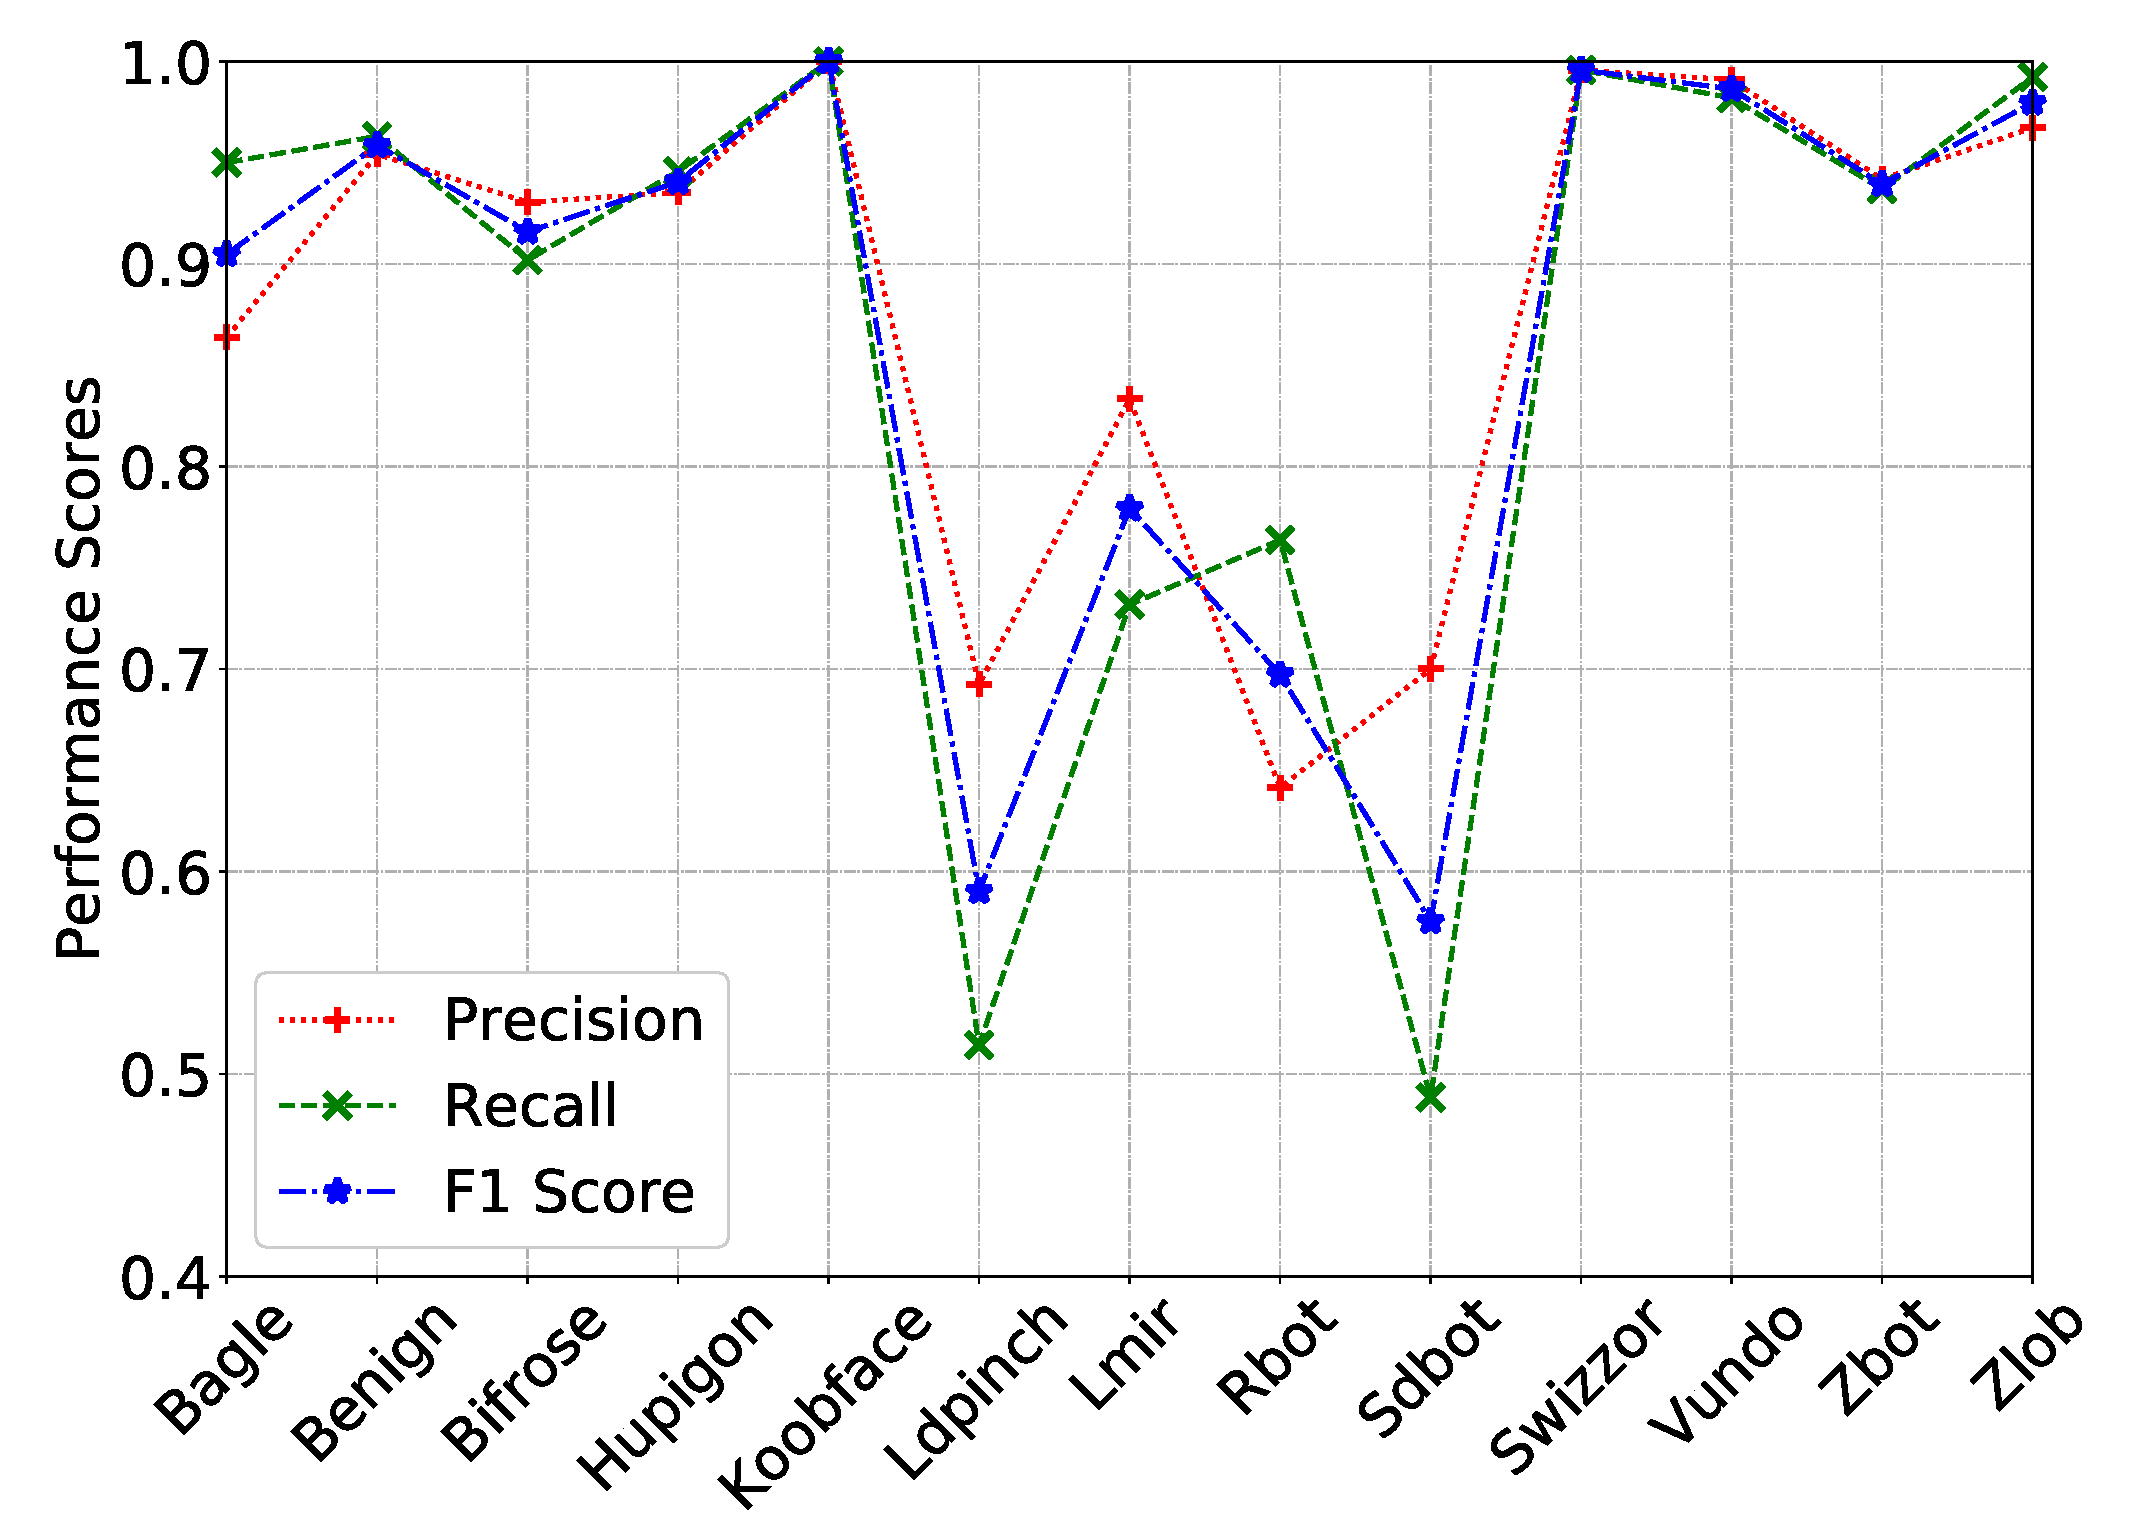
\includegraphics[width=0.48\textwidth]{Magic/figures/YanAcfgScores.eps}}
\caption{Cross-Validation Scores of \sysname on the YANCFG Dataset.}
\label{MG:Fig:YANCFGScores}
\end{figure}

\begin{figure}
\centerline{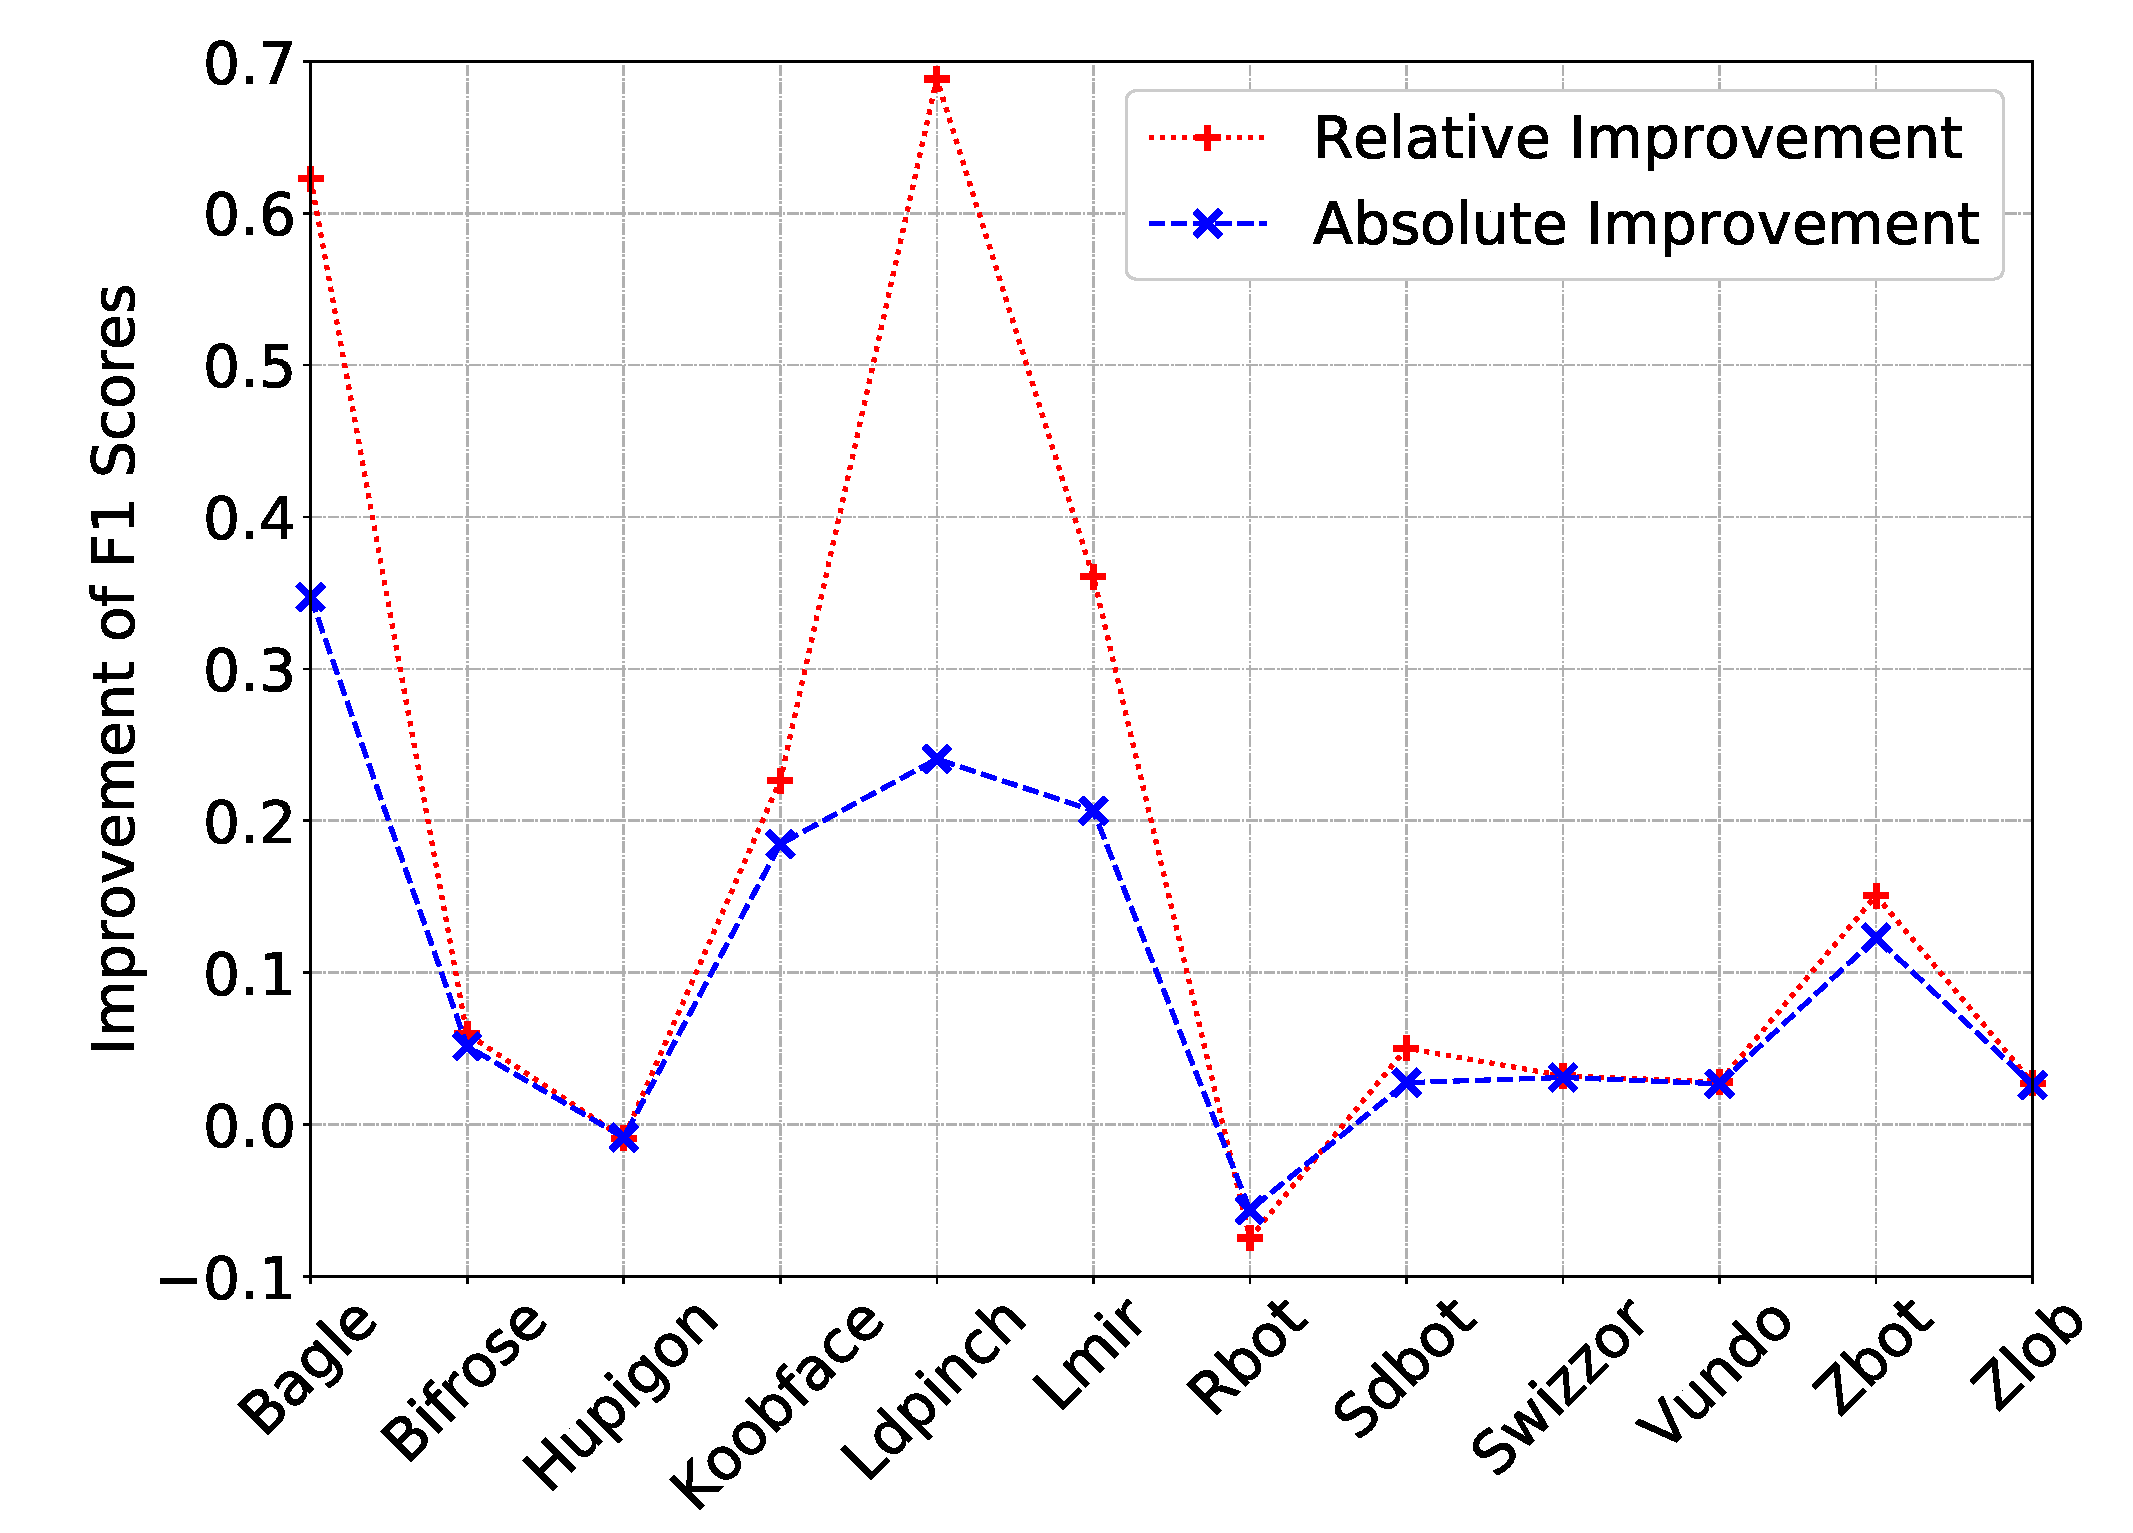
\includegraphics[width=0.48\textwidth]{Magic/figures/YanAcfgF1Improve.eps}}
\caption{F1 Score Comparison between \sysname and ESVC\cite{YanDataset} on the YANCFG Dataset.
Improvement on the classification accuracy of benign samples is not shown because it is not reported in \cite{YanDataset}.}
\label{MG:Fig:YANCFGF1Improve}
\end{figure}

% \begin{table*}
% \centering
% \caption{Confusion Matrix on the YANCFG Dataset}
% \begin{tabular}{l|rrrrrrrrrrrrr}
%   Family &  Bagle &  Benign &  Bifrose &  Hupigon &  Koobface &  Ldpinch &  Lmir &  Rbot &  Sdbot &  Swizzor &  Vundo &  Zbot &  Zlob \\
% \hline
% \hline
%     Bagle &     19 &       0 &        0 &        0 &         0 &        0 &     0 &     1 &      0 &        0 &      0 &     0 &     0 \\
%    Benign &      0 &     104 &        1 &        1 &         0 &        0 &     0 &     0 &      0 &        1 &      0 &     0 &     1 \\
%   Bifrose &      0 &       2 &      294 &       14 &         0 &        3 &     2 &     8 &      1 &        0 &      1 &     0 &     1 \\
%   Hupigon &      1 &       0 &        8 &      766 &         0 &        0 &     3 &    18 &      6 &        0 &      3 &     5 &     0 \\
%  Koobface &      0 &       0 &        0 &        0 &        20 &        0 &     0 &     0 &      0 &        0 &      0 &     0 &     0 \\
%   Ldpinch &      2 &       0 &        2 &        6 &         0 &       18 &     0 &     4 &      0 &        0 &      0 &     3 &     0 \\
%      Lmir &      0 &       2 &        0 &        7 &         0 &        1 &    30 &     1 &      0 &        0 &      0 &     0 &     0 \\
%      Rbot &      0 &       0 &        5 &       16 &         0 &        0 &     1 &    84 &      2 &        0 &      0 &     1 &     1 \\
%     Sdbot &      0 &       1 &        2 &        4 &         0 &        2 &     0 &    12 &     21 &        0 &      0 &     1 &     0 \\
%   Swizzor &      0 &       0 &        0 &        1 &         0 &        0 &     0 &     0 &      0 &      232 &      0 &     0 &     0 \\
%     Vundo &      0 &       0 &        3 &        1 &         0 &        0 &     0 &     1 &      0 &        0 &    542 &     0 &     5 \\
%      Zbot &      0 &       0 &        1 &        3 &         0 &        1 &     0 &     1 &      0 &        0 &      1 &   178 &     5 \\
%      Zlob &      0 &       0 &        0 &        0 &         0 &        1 &     0 &     1 &      0 &        0 &      0 &     1 &   384 \\
% \end{tabular}
% \label{MG:Tab:YANCFGConfusionMatrix}
% \end{table*}


\section{Conclusion} \label{sec:conclusions}
In this work, we have applied deep graph convolution neural network to the malware classification problem.
Different from existing machine learning-based malware detection approaches that commonly rely on handcrafted features and ensemble models,
this work proposes and evaluates an end-to-end malware classification pipeline with two distinguishing features.
Firstly, our malware classification system works directly on CFG-represented malware programs, making it deployable in a variety of operational environments.
%in our system, which is generic to any kind of subjects and preserves the semantic meanings of the program.
%From a CFG, one can freely define and extract attributes from each code block, thus obtaining an ACFG.
Secondly, we extend the state-of-the-art graph convolutional neural network to aggregate attributes collected from individual basic blocks through the neighborhood defined by the graph structures and thus embed them into vectors that are amenable to machine learning-based classification.
Our experimental evaluation conducted on two large malware datasets has shown that our proposed method achieves classification performances that are comparable to those of state-of-the-art methods applied on handcrafted features.

We envision MAGIC would be deployed on a cloud, as a typical end user does not have enough labeled malware samples to train good classification models.
A user can upload suspicious files to the cloud, which further trains appropriate MAGIC parameters to classify programs newly seen in her operational environment.
In this way, even if a particular user may not have labeled programs to train a specific neural network, he can still benefit from MAGIC who learns from many other uses that do have labeled datasets.

%One of the important future work for us is to conduct a cross-dataset evaluation and compare our proposed malware detection system to ensemble approaches.
%Gradient boosting approaches achieved an outstanding low loss on the Microsoft Malware Classification Challenge Dataset (corresponding to MSACFG dataset in our report),
%but their generalization ability remains untested until we apply them to more independent datasets, for example, the private dataset in our evaluation.

% \textbf{Limitation: classification on CFG/ACFG assume the input binary are unpacked assembly files.}
% How to handle packed binaries in the future?
% First, default/predefined PE sections(\textit{.text, .data, .bss, .rdata, .edata, .idata, .rsrc, .tls, and .reloc}) VS special sec names.
% Second, there are many \texttt{dd, db, dw} instructions.
\clearpage

\Chapter{Conclusions and Future Directions}
\label{Cpt:Conclusion}
\Chapter{Conclusion}
\label{Sec:Conclusion}

\section{Summary of Current Work}

Under the centre theme of securing SDN-enabled large-scale network using high-fidelity and scalable testing system, we conduct our research work in three streams.
First, we address one of the key issues in Linux-container-based network emulation (LCNE).
Even though LCNE combines many desired features of software simulation and physical testbeds,
it uses the system clock across all the containers even if a container is not being scheduled to run.
This leads to the issue of both performance and temporal fidelity, especially with high workloads.
Virtual time sheds the light on this issue by precisely scaling the time of interactions between containers and physical devices.
We develope a lightweight Linux-container-based virtual time system and integrate it to Mininet.
Except for enhancing Minint's fidelity and scalability,
our virtual time system is also an alternative for synchronizing clocks in hybrid simulation and emulation.
Second, we rethink how to simulate SDN network by taking advantage of the centralized paradigm.
Following this idea, we present a model abstraction technique that effectively transforms
the network devices in an SDN-based network to one virtualized switch model.
While significantly reducing the model execution time and enabling the real-time simulation capability,
our abstracted model also preserves the end-to-end forwarding behavior of the original network.
Third, motivated by the recent advancement and success of deep neural networks,
we study the feasibility of deep learning based network intrusion detection systems (NIDS) in order to enhance the essential network-architecture-agnostic security building-block.
We construct the detection engine with multiple advanced deep learning models and compare their performance.

\section{Future Work}
Malware detection with executable is promising
\cite{GatedConvNet, ACFG4BugSearch, GraphEmbedSimDetection, MalConvNvidia}.
%When applying the machine learning algorithms or design customized neural networks, the following
%should be taken into consideration as guidance:
%\begin{enumerate}
%\item The informative PE header of a particular Windows OS, is well-defined and also complicated.
        %Minimal domain knowledge should be relied on since they are fragile;
        %the author of the malware may intentionally leverage these rules to hide key part of the malicious code.
%\item There are high amount of positional variation presented in the executable files.
    %Since PE header 
%\end{enumerate}

\begin{algorithm}[h]
\DontPrintSemicolon
    \KwIn
    {
        $D = $ binary code dataset. \newline
        $bc = $ a particular binary code file in $D$. \newline
        $g \equiv (V, E, x) = ACFG(bc) $ the ACFG of a particular binary code file. \newline
        $\mu_v = $ feature vector of a particular node in ACFG. \newline
        $nn \equiv $ neural network with parameters $W_1, P_1, P_2, W_2$.
    }
    \SetKwProg{Fn}{Function}{}{\KwRet}
    \SetKwFunction{ACFG}{acfg\_bytecode}
    \SetKwFunction{EmbeddingACFG}{embedding\_acfg}
    \SetKwFunction{GetBatchEmbedding}{get\_batch\_embedding}
    \SetKwFunction{Train}{train}
    \Fn{\EmbeddingACFG{$g$, $nn$}} {
        Algorithm 1 in paper\;
        But return the set of vertex embeddings $\mu_g = \{\mu_v| \forall v \in V\}$\;
    }
    \Fn{\GetBatchEmbedding{$nn$}} {
        $batch\_ACFG= $ sample $batch\_size$ binary code files from $D\_ACFG$\;
        Pair $g \in batch\_ACFG$ with 1 positive and 1 negative ACFG to obtain
        $batch\_pairs = {(g_i, g_j, 1), (g_i, g_j', -1) | g_i \in batch\_ACFG}$\;
        \ForEach (// Embed $batch\_pairs$ to $batch\_embeddings$) {$(g_i, g_j, label) \in batch\_pairs$} 
        {
            $\mu_{g_i}$ = \EmbeddingACFG{$g_i$, $nn$}\;
            $\mu_{g_j}$ = \EmbeddingACFG{$g_j$, $nn$}\;
            Append $(\mu_{g_i}, \mu_{g_j}, label)$ to $batch\_embeddings$\;
        }
        \KwRet{$batch\_embeddings$}
    }
    \Fn{\Train{$D$}} {
        Initialize parameters in $nn$\;
        Convert all byte code files: $D\_{ACFG} = \{ g | g = $ \ACFG{$bc$} $\forall bc \in D\}$\;
        \For (// Train $E$ epochs) {epoch = 1 to 100} {
            \For (// Train with batch data) {i = 1 to $\frac{||D||}{batch\_size}$} {
                $batch\_embeddings = $ \GetBatchEmbedding{$nn$}\;
                $nn$.fit($batch\_embeddings$)\;
            }
        }
    }
\caption{End-to-End Traning Algorithm with Embedding}
\end{algorithm}


%
% APPENDIX
%
% Do the settings of appendices with \appendix command
% \appendix

% Then create each appendix using
% \Appendix{title_of_appendix} command
%
% BIBLIOGRAPHY
%
% you have two options: 1) create bibliography manually,
% 2) create bibliography automatically. See BibliographyHelp.pdf file for details.
\Urlmuskip=0mu plus 1mu\relax
\bibliographystyle{ieee}
\bibliography{mybib}

\end{document}  % end of document
